\bookpart{实数与一元函数}{Real Numbers And Univariate Functions}
\label{part:calculus}
\label{part:calculus-and-optimization}

\BookPartGuide{%
函数可以描述一个量怎样随另一个量变化，但要讨论输入逐渐靠近某一点时的行为，先需要准确说明“趋近”。对于无限累计，我们还要判断部分和是否趋于确定的值；即使知道一组函数值有下界，也不能因此断定某个输入取得最小值。

第~\ref{chap:function-limits}章从实值函数的运算与实数的确界出发，用误差条件定义数列与函数的极限，并以部分和的极限建立级数；实数完备性为判断极限是否存在提供依据。章末讨论实轴上的邻域、开闭集和闭区间的紧致性，为研究函数的局部与整体性质作准备。

第~\ref{chap:univariate-differentiation}章研究连续性、导数与微分，说明如何由一点附近的变化率得到区间上的信息。第~\ref{chap:univariate-integration}章从集合的测量进入积分，比较黎曼积分与勒贝格积分，并讨论积分与微分、极限之间的关系。阅读时应区分局部变化与累计，也要留意交换极限和积分所需的条件。}

\chapter{函数的极限}
\label{chap:function-limits}
\label{chap:mathematical-analysis}

第~\ref{chap:sets-functions-and-proofs}章的等比递推给出了有限步结果$e^{(t)}=\rho^te_0$；
当$t$无限增大时，这些数是否趋向确定的值？有限几何和在项数增加时又怎样变化？
回答这类问题，先要说清“趋近”是什么意思，还要知道实数集合在什么条件下有最小的上界。

本章先说明实值函数的逐点运算与函数族，建立实数的确界、完备性与函数的最值；再用误差条件定义数列的极限，
区分已知收敛时怎样计算极限与不知道极限值时怎样保证极限存在，后者要用到实数的确界原理。
级数是部分和组成的数列，数列极限的结论由此用于无限多项的累计，并引出重排与分组这些有限和中不会出现的问题。
随后把极限从数列推广到函数，用输入的距离控制输出的误差，并借序列判据沿用数列的运算法则。
最后讨论实轴上的邻域、开闭集与闭区间的有限子覆盖性质，为一元微积分中的局部与整体分析作准备。

\section{实值函数及其界}
\label{sec:real-valued-functions-bounds}

第~\ref{chap:sets-relations-maps}章的映射可以取值于任意集合。本章研究的数列与函数都取实数值，
实数既能相加相乘，又能比较大小：前者使函数之间可以逐点运算，后者引出“能取到多小的值”这类问题。
极限存在与否，最终也要回到实数集合有没有最小的上界。本节先说明实值函数的逐点运算，
再把整个函数作为集合的元素，讨论用参数编号的函数族；最后建立实数集合的确界、实数的完备性与函数的最值，
它们是下一节判断极限存在的依据。

\subsection{实值函数的运算}
\label{sec:real-function-arithmetic}

若$f,g:X\to\mathbb R$有相同定义域，可以在每个输入处计算函数值的和、差、积：
\[
 \begin{aligned}
 (f+g)(x)&=f(x)+g(x),\\
 (f-g)(x)&=f(x)-g(x),\\
 (fg)(x)&=f(x)g(x).
 \end{aligned}
\]
对实常数$c$，定义
\[
  (cf)(x)=cf(x).
\]
这些新函数的定义域仍是$X$。

商函数则只在分母不为零的范围内定义：
\[
  (f/g)(x)=f(x)/g(x),
\]
其定义域为$\{x\in X:g(x)\neq0\}$。例如在$\mathbb R$上取$f(x)=x$、$g(x)=x-1$，则$(f+g)(x)=2x-1$定义在整个实轴上，
而$(f/g)(x)=x/(x-1)$的定义域不含$1$。
与复合不同，逐点运算要求两个函数有相同的定义域，并在每个输入处对两个函数值做实数运算；
复合则把一个函数的输出作为另一个函数的输入，见第~\ref{sec:prelim-map-operations}节。

\subsection{函数族与参数化}
\label{sec:prelim-function-families}

\paragraph{函数族}
设想由输入预测输出：事先并不知道哪条规则最合适，通常先划定一批候选规则，再从中挑选。
这批候选规则本身是一个集合，它的元素是整个函数。
具有同一定义域和陪域的一组函数组成函数族（family of functions）。

例如，形如$f(x)=ax+b$的函数称为一元仿射函数（affine function），所有这样的函数组成
\[
 \mathcal F=\{f_{a,b}:\mathbb R\to\mathbb R:\ f_{a,b}(x)=ax+b,\ (a,b)\in\mathbb R^2\}.
\]
族中的每个元素是一整个函数。取$(a,b)=(2,1)$得到函数$f_{2,1}(x)=2x+1$；
再取输入$x=3$，才得到一个函数值$f_{2,1}(3)=7$。

\paragraph{函数参数化}
用参数为函数族中的函数编号，称为参数化（parameterization）。
一般写成$\theta\mapsto f_\theta$，其中$\theta$属于参数集合$\Theta$，
$f_\theta:X\to Y$是相应的函数。
映射$\theta\mapsto f_\theta$的输入是参数，输出是函数；函数$f_\theta$自身的输入仍是$x$。
在上例中，$\theta=(a,b)$指定一条直线，而$x$指定在直线上的哪个位置求值。
参数化把“在函数中挑选”改写为“在参数集合中挑选”；参数集合通常是$\mathbb R^2$这样熟悉的集合，
便于后续用数值方法比较和调整。

\paragraph{函数参数化的可识别性}
不同参数可能表示同一个函数，所以参数与函数未必一一对应。能否由函数反过来确定参数，取决于下面的条件。
\begin{definition}[函数参数化的可识别性]
\label{def:prelim-identifiable-parameterization}
给定参数集合$\Theta$与函数族$\{f_\theta:X\to Y:\theta\in\Theta\}$。
若$f_\theta=f_{\theta'}$蕴含$\theta=\theta'$，即$\theta\mapsto f_\theta$为单射，
则称这一函数参数化可识别（identifiable）；也就是说，完整函数唯一确定其参数。
否则称为不可识别。
\end{definition}
这里比较的是整个定义域上的函数，而非几个位置的函数值。
例如仿射函数族中$b=f_{a,b}(0)$、$a=f_{a,b}(1)-f_{a,b}(0)$，
所以完整函数唯一确定$(a,b)$，这一参数化可识别。若只观察$x=0$处的函数值，则只能确定$b$，
不能确定$a$。可见，有限个观测是否足以确定参数，与参数化是否可识别是两个不同的问题。

\Needspace{11\baselineskip}
\begin{example}[参数不同而函数相同]
\label{ex:prelim-nonidentifiable-parameterization}
考虑参数化函数
\[
  f_{a,b}:\mathbb{R}\to\mathbb{R},
  \qquad
  f_{a,b}(x)=abx,
  \qquad
  (a,b)\in\mathbb{R}^2.
\]
参数$(1,2)$与$(2,1)$不同，却对每个$x$给出相同的函数值。更一般地，只要$c\neq0$，
$(ca,b/c)$与$(a,b)$就表示同一个函数。从完整的输入输出关系可以确定乘积$ab$（例如取$x=1$，有$ab=f_{a,b}(1)$），
却不能分别确定$a$和$b$。这是参数化本身不可识别，而不是计算精度不足。
\end{example}


图~\ref{fig:vol1-add-parameter-function-value}把“由参数得到函数”和“由函数得到函数值”这两层操作分开：三组不同参数先汇入同一条完整规则，然后才在指定的$x$处求值。
\begin{figure}[!htb]
  \centering
  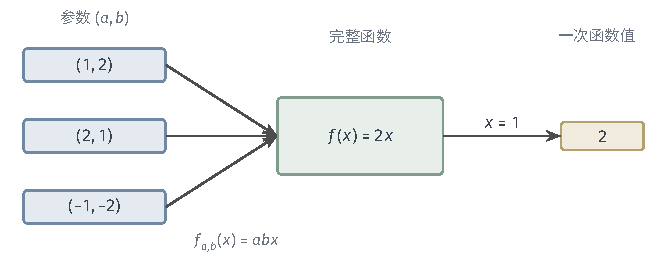
\includegraphics[width=112mm]{figures/00-shared/mathematical-preliminaries-upper/00-shared/tikz/mathematical-language-combinatorics-analysis-optimization-comprehension-additions/parameter-function-value.pdf}
  \caption{参数化$f_{a,b}(x)=abx$中的三层对象。参数$(1,2),(2,1),(-1,-2)$的乘积均为$2$，所以它们表示同一个函数$f(x)=2x$；再指定$x=1$，才得到一次求值结果$2$。多组参数汇入同一完整函数，正是不可识别性。}
  \label{fig:vol1-add-parameter-function-value}
\end{figure}

不可识别的参数可以用第~\ref{sec:prelim-equivalence-relations}节的等价关系整理。规定$\theta\sim\theta'$当且仅当$f_\theta=f_{\theta'}$，
就得到参数集合上的等价关系：函数相等本身是反身、对称、传递的，三条性质直接继承。
每个等价类收集同一个函数的全部参数表示；在$f_{a,b}(x)=abx$中，$(a,b)$所在的等价类是满足$a'b'=ab$的全部参数$(a',b')$。

把每个等价类对应到它所表示的函数，就得到从商集$\Theta/{\sim}$到函数族$\{f_\theta:\theta\in\Theta\}$的双射。
参数化可识别，恰好意味着每个等价类只含一个参数。
换言之，函数族中的元素按函数区分，参数则可能为同一个函数保留多种表示。

\subsection{实值函数的界与极值}
\label{sec:prelim-optimal-values-errors}

从候选函数中挑选时，常把每个候选的优劣写成一个实数，例如预测误差，再寻找使它最小的候选。
这就要求讨论一个实值函数能取到多小的值、最小值是否真的取得。
函数值组成实数集合，而实数的通常大小$\leq$是全序。下面先把偏序集合中的界用于实数并定义确界，
说明保证确界存在的实数完备性，再把这些概念用于函数。

\paragraph{上界与下界}
设$A\subseteq\mathbb R$非空。若$a\leq M$对每个$a\in A$成立，
就称$M$为$A$的上界（upper bound）；若$m\leq a$对每个$a\in A$成立，
就称$m$为下界（lower bound）。这正是第~\ref{sec:prelim-order-relations}节偏序集合中上界、下界的定义在$(\mathbb R,\leq)$中的情形。
存在上界称为上有界，存在下界称为下有界，两者都有称为有界。
例如$(0,1)$有上界$1,2$，也有下界$0,-1$。界不必是集合中的元素，也不唯一。

\paragraph{上确界与下确界}
上界中的最小者称为\term{上确界}（supremum），记作$\sup A$；
下界中的最大者称为\term{下确界}（infimum），记作$\inf A$。
例如$\sup(0,1)=1$、$\inf(0,1)=0$，两个确界都不属于$(0,1)$。

上确界$\beta$不仅要满足$a\leq\beta$对所有$a\in A$成立，
还要满足每个$\varepsilon>0$都存在$a\in A$使$a>\beta-\varepsilon$。
后一个条件说明，任何比$\beta$小的数都不是上界。
下确界$\alpha$类似地满足$\alpha\leq a$对所有$a\in A$成立，且每个$\varepsilon>0$都存在$a\in A$
使$a<\alpha+\varepsilon$。

一个集合一旦有上界，就有无限多个上界；其中是否存在最小的一个，不能从上界的定义直接看出。
本书把下面的性质作为实数的基本性质使用，称为实数的完备性（也称确界原理）：
非空上有界实数集合有实数上确界，非空下有界实数集合有实数下确界。
有理数没有这一性质：集合$\{q\in\mathbb Q:q^2<2\}$在有理数中有上界（例如$2$），
但它在实数中的上确界是$\sqrt2$，而$\sqrt2$不是有理数。于是每个有理上界都严格大于$\sqrt2$，
在它与$\sqrt2$之间总还有更小的有理上界，所以在有理数中找不到最小的上界。
实数补上了这样的“空隙”，后面关于极限存在的结论都要用到这一点。

\paragraph{函数的有界性}
对非空定义域$X$上的实值函数$f:X\to\mathbb R$，讨论其有界性就是讨论值域$f(X)$的有界性。
例如$f(x)=x$在$(0,1)$上有界，在$\mathbb R$上则既无上界也无下界。
值域的确界简记为
\[
 \inf_{x\in X}f(x)=\inf f(X),\qquad
 \sup_{x\in X}f(x)=\sup f(X).
\]
若$f(X)$无下界，约定其下确界为$-\infty$；若无上界，约定其上确界为$+\infty$。
这两个符号表示没有有限的界，不是实值函数实际取到的数。

\paragraph{最小值与最小点}
若存在$x^\star\in X$使
\[
 \forall x\in X,\qquad f(x^\star)\leq f(x),
\]
则称$x^\star$为\term{全局最小点}（global minimizer），$f(x^\star)$为最小值。
符号$\forall$读作“对所有”，这里要求与定义域内的每个函数值比较。
最小值记作$\min_{x\in X}f(x)$；全部最小点组成的集合记作
\[
 \argmin_{x\in X}f(x)
 =\{x\in X:\ f(x)\leq f(z)\text{ 对所有 }z\in X\}.
\]
$\min$给出一个数，$\argmin$给出输入的集合；若不存在最小点，后一个集合为空。

最小值存在时必等于下确界：$f(x^\star)$不超过每个函数值，所以是值域的一个下界；
任何下界$m$都满足$m\leq f(x^\star)$，因为$f(x^\star)$本身就是一个函数值。
所以$f(x^\star)$是最大的下界。反过来，下确界存在却未必被取得。
例如$f(x)=x$在$(0,1)$上的下确界为$0$，但没有最小点，
因为任意允许的$x$都有更小的允许输入$x/2$。

\paragraph{最大值与最大点}
若存在$x^\star\in X$使$f(x^\star)\geq f(x)$对所有$x\in X$成立，
则称$x^\star$为全局最大点，$f(x^\star)$为最大值。
最大值记作$\max_{x\in X}f(x)$，全部最大点组成
\[
 \argmax_{x\in X}f(x)
 =\{x\in X:\ f(x)\geq f(z)\text{ 对所有 }z\in X\}.
\]
与最小值的论证对称，最大值存在时等于上确界。函数$f(x)=x$在$(0,1)$上没有最大值；
将定义域换为$[0,1]$后，最大值为$1$、最大点为$1$，最小值为$0$、最小点为$0$。

\begin{example}[同一个最优值可以对应多个输入]
\label{ex:prelim-optimal-value-versus-points}
令$X=[-2,2]$，$f(x)=(x^2-1)^2$。平方非负，且$x=\pm1$都使它为零，所以
\[
  \min_{x\in X}f(x)=\inf_{x\in X}f(x)=0,\qquad
  \argmin_{x\in X}f(x)=\{-1,1\}.
\]
又因为$0\leq x^2\leq4$，有$|x^2-1|\leq3$，于是$f(x)\leq9$，等号恰在$x=\pm2$
处成立。因此最大值为$9$，最大点集合为$\{-2,2\}$。最小值是一个数，不会因为有两个
最小点就变成两个最小值；最优点是否唯一是另一个问题。
\end{example}

图~\ref{fig:prelim-minimum-infimum}固定表达式$f(x)=x$，比较它在$(0,1)$与$[0,1]$上定义的两个函数。
两侧的函数值都以$0$为下确界；右侧把$x=0$纳入定义域后，这个下确界才由某个输入取得。
区别的关键在于边界点是否属于定义域，而不在于两条曲线是否趋向同一个高度。

\begin{figure}[htbp]
  \centering
  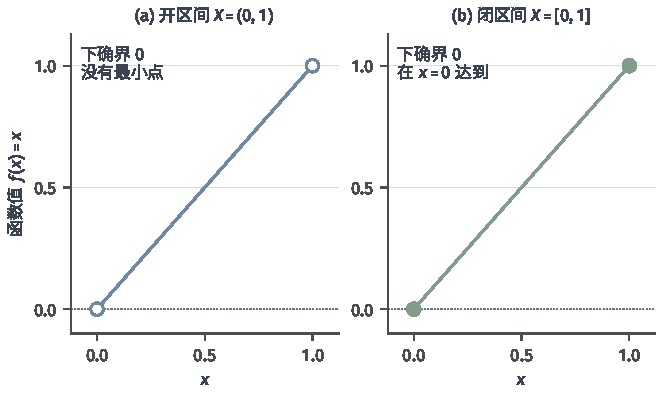
\includegraphics[width=112.0mm]{figures/00-shared/mathematical-preliminaries-upper/01-mathematical-language-combinatorics-analysis-optimization/matplotlib/prelim-minimum-infimum/figure.pdf}
  \caption{同一求值表达式$f(x)=x$在两个定义域上的边界对照。左图定义域为$(0,1)$，空心端点不属于图像，函数值可任意接近$0$，却不能取到；右图定义域为$[0,1]$，实心端点$(0,0)$达到下确界。两图的下确界相同，最小点是否存在取决于可行端点是否保留。图为解析教学示例。}
  \label{fig:prelim-minimum-infimum}
\end{figure}
\FloatBarrier

\section{序列的极限}
\label{sec:analysis-continuous-limits}

数列$1,1/2,1/3,\ldots$越来越接近$0$，数列$-1,1,-1,1,\ldots$则在两个值之间来回交替。
直觉上前者“有极限”，后者没有；但“越来越接近”需要精确的含义，否则无法判断更复杂的情形，
例如$(1+1/n)^n$或$\sum_{k\leq n}1/k$是否趋向某个数。
极限用误差条件给出这种含义：给定任意小的误差，后面的项是否都能落在这一误差范围内。

\label{sec:analysis-sequences-series-errors}

有了定义以后，还要回答两类问题：已知几个数列收敛时，怎样计算由它们组合出的数列的极限；
尚不知道极限值时，怎样从数列本身的性质保证极限存在。前者借助极限的运算法则与夹逼，
后者依靠单调有界、收敛子列和柯西准则，这三种判别都要用到第~\ref{sec:prelim-optimal-values-errors}节的确界原理。
本节先定义收敛并说明收敛数列有界，再建立存在性判别，然后讨论极限的唯一性、运算与夹逼，
最后用上、下极限描述不收敛数列尾部的上下边界。

\subsection{数列的收敛}

\paragraph{收敛与发散}
数列$(a_n)_{n\geq1}$是一列按正整数排列的实数。
“接近一个数”要同时约束后面的全部项，不能只看某几个位置：$((-1)^n)$的偶数项都等于$1$，
但奇数项始终离$1$有距离$2$，所以它不应算作趋于$1$。
只要求“各项与$a$的距离越来越小”也不够，例如$1+1/n$离$0$越来越近，却始终大于$1$。
合适的要求是：无论事先给定多小的正误差，从某一项起，后面\emph{每一项}与$a$的距离都小于这个误差。

若存在$a\in\mathbb R$，使每个$\varepsilon>0$都对应一个正整数$N$，满足
\[
 n\geq N\quad\Longrightarrow\quad |a_n-a|<\varepsilon,
\]
就称$(a_n)$\term{收敛}（converge）到$a$，$a$称为其极限，记作
$\lim_{n\to\infty}a_n=a$或$a_n\to a$。没有有限实数极限时，称数列发散（diverge）。
这里先任给误差$\varepsilon$，再选取$N$；选定以后，所有$n\geq N$都须满足要求。
$N$可以依赖于$\varepsilon$，误差要求越严格，所需的尾部起点通常越靠后；定义也不要求这个$N$唯一。
极限不要求某一项恰好等于$a$\scite{math-lebl-analysis1}。

例如对$a_n=1/n$，任给$\varepsilon>0$，取正整数$N>1/\varepsilon$，则$n\geq N$时
$|a_n-0|=1/n\leq1/N<\varepsilon$，所以$1/n\to0$。这样的整数$N$一定存在，因为正整数集合没有上界：
否则它有上确界$s$，而$s-1$不是上界，存在正整数$k>s-1$，于是正整数$k+1>s$，矛盾。

反过来，要说明$((-1)^n)$不收敛到任何$a$，只需取$\varepsilon=1$：
相邻两项相差$2$，不可能同时落在长度为$2$的开区间$(a-1,a+1)$内，所以没有$N$能使后面全部项满足要求。

图~\ref{fig:analysis-process-sequence-tail}把“全部尾部项”画成同一条误差带：选定起点以后，后面每一项都必须留在带内。
\begin{figure}[!htbp]
 \centering
 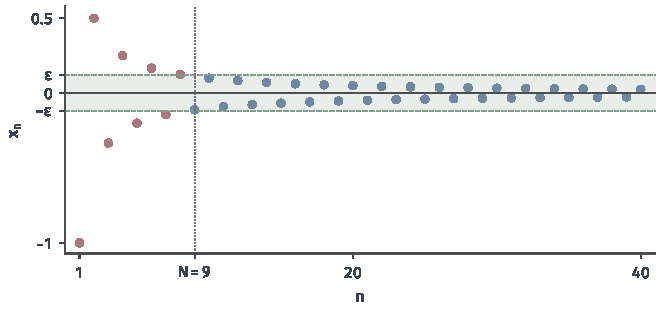
\includegraphics[width=112.0mm]{figures/00-shared/mathematical-preliminaries-upper/00-shared/matplotlib/chapter3-concept-processes/sequence-tail.pdf}
 \caption{数列$x_n=(-1)^n/n$的前40项。绿色带为$|x_n|<0.12$，取$N=9$后，所有$n\geq9$都在带内；蓝点标记这个尾部，红点标记之前的项。尾部条件针对无限多个$n$，其成立依据是$1/n\leq1/9<0.12$，不是只检查图中有限个点。}
 \label{fig:analysis-process-sequence-tail}
\end{figure}

\paragraph{收敛数列的有界性}
收敛的定义只控制尾部，但尾部之前只有有限个项，因此收敛数列必有界。
设$a_n\to a$，取$\varepsilon=1$，得到$N$使$n\geq N$时$|a_n-a|<1$，从而$|a_n|<|a|+1$。
令$M=\max\{|a_1|,\ldots,|a_{N-1}|,|a|+1\}$，便有$|a_n|\leq M$对所有$n$成立。

反向结论不成立，例如$((-1)^n)$有界却不收敛：有界性只限制取值范围，没有控制尾部是否还在振荡。
这一性质常以逆否形式使用：无界数列一定发散。下一小节将看到，
有界性再配合单调性，或者只要求选出一部分项，就能得到收敛的结论。

\subsection{数列的收敛判别}

定义收敛时需要指定一个候选极限，但很多数列的候选极限尚不明确。
下面依次利用变化方向、取值范围和尾部各项的互相接近来判断极限是否存在，并说明各自需要的条件。

\subsubsection{单调数列的收敛}
若对所有$n$都有$a_n\leq a_{n+1}$，称数列单调不减；
若总有$a_n\geq a_{n+1}$，称数列单调不增，两者统称为单调数列。

对于单调不减且有上界的数列，第~\ref{sec:prelim-optimal-values-errors}节的确界原理
为全部项提供一个最小上界；单调性则保证后面的项一直靠近它。
\begin{theorem}[单调有界收敛定理]
\label{thm:analysis-monotone-bounded-sequence}
设$(a_n)_{n\geq1}$为实数列。
若$a_n\leq a_{n+1}$对所有$n\geq1$成立，且存在$M\in\mathbb R$使$a_n\leq M$对所有$n\geq1$成立，则
\[
 \lim_{n\to\infty}a_n=\sup\{a_n:n\geq1\}\in\mathbb R.
\]
若$a_n\geq a_{n+1}$对所有$n\geq1$成立，且存在$m\in\mathbb R$使$a_n\geq m$对所有$n\geq1$成立，则
\[
 \lim_{n\to\infty}a_n=\inf\{a_n:n\geq1\}\in\mathbb R.
\]
\end{theorem}
\begin{proof}
设$a=\sup\{a_n:n\geq1\}$。给定$\varepsilon>0$，$a-\varepsilon$不是上界，
所以存在$N$使$a_N>a-\varepsilon$。单调性使$n\geq N$时都有
$a-\varepsilon<a_N\leq a_n\leq a$，这正是$a_n\to a$。
单调不增的情形对$-a_n$应用同一论证。
\end{proof}
证明中只有一处用到实数的\term{完备性}（completeness）：非空上有界的实数集合$\{a_n:n\geq1\}$有实数上确界。
两个条件都不能省去：$(n)$单调却无上界，$((-1)^n)$有界却不单调。
结合收敛数列的有界性可知，单调数列收敛当且仅当它有界。

\subsubsection{有界数列的子序列收敛}
数列可能整体不收敛，但其中一些项仍有共同的趋向。保持原有次序选出一部分项，
得到子序列（subsequence），也称子列：若$n_1<n_2<\cdots$为严格递增的正整数列，
则$(a_{n_k})_{k\geq1}$为$(a_n)$的子序列。由归纳可知$n_k\geq k$。

收敛数列的每个子序列都收敛到同一极限：若$n\geq N$时$|a_n-a|<\varepsilon$，
则$k\geq N$时$n_k\geq k\geq N$，同一误差界仍然适用。
反过来，一个子序列收敛不能保证原数列收敛；$((-1)^n)$的偶数项恒为$1$，奇数项恒为$-1$。

有界数列未必收敛，但有界性能保证从中选出一个收敛子序列。
这一结论称为Bolzano--Weierstrass定理，随后将用它证明柯西条件足以保证实数列收敛。
\begin{theorem}[Bolzano--Weierstrass定理]
\label{thm:analysis-bounded-subsequence}
设$(a_n)_{n\geq1}$为实数列。若存在$M\geq0$使$|a_n|\leq M$对所有$n\geq1$成立，
则存在严格递增的正整数列$n_1<n_2<\cdots$和$a\in\mathbb R$，使
\[
 \forall\varepsilon>0,\quad\exists K\in\{1,2,\ldots\},\quad
 k\geq K\Longrightarrow |a_{n_k}-a|<\varepsilon.
\]
即$a_{n_k}\to a$。
\end{theorem}
\begin{proof}
从包含全部项的闭区间$I_0=[-M,M]$出发，将它平分，两半中至少有一半含有无穷多个下标对应的项；
选出这一半，再重复平分与选择，得到嵌套闭区间$I_0\supseteq I_1\supseteq\cdots$，
其中$I_k=[l_k,r_k]$含有无穷多项，长度为$2M\cdot2^{-k}$。
由$2^k\geq k+1$，这些长度至多为$2M/(k+1)$，因而趋于零；这里不必先用后面的等比数列极限。
由于每个$I_k$都含有无穷多项，可以依次选取下标$n_1<n_2<\cdots$，使$a_{n_k}\in I_k$。

再确定子序列的极限。各左端点$l_k$单调不减，而由嵌套性，每个$r_j$都是全部左端点的上界。
由确界原理，$c=\sup_k l_k$存在，并满足$l_k\leq c\leq r_k$对每个$k$成立。
给定$\varepsilon>0$，先选$K$使$r_K-l_K<\varepsilon$；
当$k\geq K$时，$a_{n_k}\in I_k\subseteq I_K$，且$c\in I_K$，所以$|a_{n_k}-c|\leq r_K-l_K<\varepsilon$。
\end{proof}

\subsubsection{柯西数列的收敛}
单调条件并不适用于所有收敛数列。若还不知道候选极限，可以检查尾部各项是否彼此接近。
满足
\[
 \forall\varepsilon>0,\quad\exists N,\quad
 \forall m,n\geq N,\quad |a_m-a_n|<\varepsilon
\]
的数列称为\term{柯西数列}（Cauchy sequence）。对实数列，这个条件与收敛等价。
\begin{theorem}[柯西收敛准则]
\label{thm:analysis-cauchy-convergence}
设$(a_n)_{n\geq1}$为实数列。存在$a\in\mathbb R$使$a_n\to a$，当且仅当
\[
 \forall\varepsilon>0,\quad\exists N\in\{1,2,\ldots\},\quad
 \forall m,n\geq N,\quad |a_m-a_n|<\varepsilon.
\]
\end{theorem}
\begin{proof}
每个收敛实数列都是柯西数列：若$n\geq N$时$|a_n-a|<\varepsilon/2$，则对$m,n\geq N$，
$|a_m-a_n|\leq|a_m-a|+|a_n-a|<\varepsilon$。

反过来，柯西条件先保证数列有界，论证与收敛数列的有界性相同，只是把极限换成尾部中的一项：
取误差$1$，所有$n\geq N$都满足$|a_n-a_N|<1$，前面有限个项另取最大绝对值即可。
由Bolzano--Weierstrass定理，可取子序列$a_{n_k}\to a$。

给定$\varepsilon>0$，选$N$使任意$m,n\geq N$满足$|a_m-a_n|<\varepsilon/2$，
再选一个$k$，使$n_k\geq N$且$|a_{n_k}-a|<\varepsilon/2$。
于是每个$n\geq N$都有
$|a_n-a|\leq|a_n-a_{n_k}|+|a_{n_k}-a|<\varepsilon$。
\end{proof}
这一准则的充分性通过收敛子列，仍然依赖实数的确界原理。

验证柯西条件时，可把两个较晚的项之间的距离估计为逐步变化的总和。对$m>n$，
\begin{equation}
 |a_m-a_n|\leq\sum_{k=n}^{m-1}|a_{k+1}-a_k|.
\label{eq:analysis-cauchy-tail-bound}
\end{equation}
仅有相邻差趋零还不够，因为中间的步数也在增加，必须控制整段和。
例如$a_1=0$、$a_{k+1}-a_k=1/k$时，每一步都趋零，但$a_{2n}-a_n=\sum_{k=n}^{2n-1}1/k$共有$n$项，
每项都大于$1/(2n)$，所以$a_{2n}-a_n>1/2$，它不是柯西数列，因而发散。
这里的$a_{n+1}$正是第~\ref{sec:analysis-series}节调和级数的前$n$项和：每一项都变小，累计却不稳定。

\subsection{极限的基本性质}

前面的判别给出了保证收敛的条件。现在假定实数列已经收敛，先说明极限唯一，
再分别计算和、差、数乘、积与商的极限，最后说明怎样用上下界夹逼求极限。
这些运算法则都以有限极限存在为前提，不能代替收敛性的判别。

\paragraph{极限的唯一性}
收敛数列的极限是唯一的。若$a\neq b$都是极限，
取$\varepsilon=|a-b|/3$，充分靠后的项应同时满足
$|a_n-a|<\varepsilon$和$|a_n-b|<\varepsilon$；
三角不等式却给出$|a-b|\leq|a-a_n|+|a_n-b|<2|a-b|/3$，矛盾。
因此记号$\lim_{n\to\infty}a_n$表示一个确定的数。

\paragraph{和的极限}
实际计算时，一个数列常由几个已知数列相加得到。设$a_n\to a$、$b_n\to b$，其中$a,b\in\mathbb R$，则
\[
 \lim_{n\to\infty}(a_n+b_n)=a+b.
\]
因为$|(a_n+b_n)-(a+b)|\leq|a_n-a|+|b_n-b|$，
只需让两个误差分别小于$\varepsilon/2$，便能使和的误差小于$\varepsilon$。

\paragraph{差的极限}
相减时也可以分别控制两列数的误差。在同样的有限收敛条件下，
\[
 \lim_{n\to\infty}(a_n-b_n)=a-b.
\]
这来自$|(a_n-b_n)-(a-b)|\leq|a_n-a|+|b_n-b|$，取尾部起点使右侧两项各小于$\varepsilon/2$即可。

\paragraph{数乘的极限}
把每一项乘以固定的实数$c$，只会把误差乘以$|c|$，所以
\[
 \lim_{n\to\infty}ca_n=ca.
\]
$c=0$时结论直接成立；$c\neq0$时，把原数列误差控制在$\varepsilon/|c|$以内即可。

\paragraph{积的极限}
乘积的误差还包含一个变化的因子，需要用到收敛数列的有界性。若$a_n\to a$、$b_n\to b$，则
\[
 \lim_{n\to\infty}a_nb_n=ab.
\]
取$M\geq1$使所有$|a_n|\leq M$，把误差拆成两部分：
\[
 |a_nb_n-ab|=|a_n(b_n-b)+b(a_n-a)|\leq M|b_n-b|+|b|\,|a_n-a|.
\]
让$|b_n-b|<\varepsilon/(2M)$、$|a_n-a|<\varepsilon/[2(|b|+1)]$同时成立，右侧便小于$\varepsilon$。

\paragraph{商的极限}
除法还须避免分母趋零。若$a_n\to a$、$b_n\to b$且$b\neq0$，则充分靠后的$b_n\neq0$，并且
\[
 \lim_{n\to\infty}\frac{a_n}{b_n}=\frac ab.
\]
事实上，取误差$|b|/2$，可知充分靠后的$|b_n|\geq|b|/2$，于是
$|1/b_n-1/b|=|b_n-b|/(|b_n||b|)\leq2|b_n-b|/|b|^2$，右侧趋于零；
前面有限个项不影响极限，再对$a_n\cdot(1/b_n)$用乘积规则即得结论。
例如将分子分母同除以$n$，得$n/(n+1)=1/(1+1/n)\to1$。
分母趋于零时不能套用此式：$0/0$与$\infty-\infty$一样，都不是可以直接计算的数值。

\paragraph{夹逼定理}
有时中间数列不断振荡，直接控制它的误差并不方便，但可以分别找到上下界。
若上下两列最终都靠近同一有限值，中间数列便被限制在同一误差范围内。
\begin{theorem}[夹逼定理]
\label{thm:analysis-sequence-squeeze}
设$(a_n)$、$(b_n)$、$(c_n)$为实数列。若存在正整数$N_0$使
\[
 \forall n\geq N_0,\qquad a_n\leq c_n\leq b_n,
\]
并且存在$\ell\in\mathbb R$满足
$\lim_{n\to\infty}a_n=\lim_{n\to\infty}b_n=\ell$，则
$\lim_{n\to\infty}c_n=\ell$。
\end{theorem}
\begin{proof}
任给$\varepsilon>0$，由两端收敛可选正整数$N_1,N_2$，使
$n\geq N_1$时$|a_n-\ell|<\varepsilon$，$n\geq N_2$时$|b_n-\ell|<\varepsilon$。
取$N=\max\{N_0,N_1,N_2\}$，则每个$n\geq N$都有
\[
 \ell-\varepsilon<a_n\leq c_n\leq b_n<\ell+\varepsilon.
\]
所以$|c_n-\ell|<\varepsilon$，按定义即$c_n\to\ell$。
\end{proof}
例如$-1/n\leq(\sin n)/n\leq1/n$，所以$(\sin n)/n\to0$。

一个反复使用的例子是$|r|<1$时$r^n\to0$。$r=0$时直接成立；
若$0<|r|<1$，写$1/|r|=1+h$，其中$h>0$。
先用归纳法证明$(1+h)^n\geq1+nh$：$n=1$时取等号；若它对$n$成立，则
$(1+h)^{n+1}\geq(1+nh)(1+h)=1+(n+1)h+nh^2\geq1+(n+1)h$。
因此$0<|r|^n\leq1/(1+nh)<(1/h)\cdot(1/n)\to0$，
再对$-|r|^n\leq r^n\leq|r|^n$用夹逼定理，得到$r^n\to0$。

这回答了章首关于等比递推~\eqref{eq:prelim-geometric-recurrence}的问题：
$|\rho|<1$时$e^{(t)}=\rho^te_0\to0$。另几种情形同样可以判断：设$e_0\neq0$，
$\rho=1$时各项恒为$e_0$；$\rho=-1$时各项在$\pm e_0$间交替，不收敛；
$|\rho|>1$时，同一不等式给出$|\rho|^t\geq1+th$（其中$|\rho|=1+h$），数列无界，因而发散。

\subsection{数列的上极限与下极限}
数列不收敛时，仍可考察其尾部的上下边界。
为记录无界的趋向，约定$a_n\to+\infty$表示对每个实数$M$，充分大的$n$都满足$a_n>M$；
$a_n\to-\infty$则要求最终都有$a_n<M$。
这两个符号不是有限实数极限，$\overline{\mathbb R}=\mathbb R\cup\{-\infty,+\infty\}$称为扩展实数，
其中$\infty-\infty$没有定义。

逐渐舍去前项时，尾部下界只会上升，尾部上界只会下降，因此可以分别用单调数列的极限记录它们。
\begin{definition}[数列的上极限与下极限]
\label{def:analysis-liminf-limsup}
对扩展实数列$(a_n)$，定义
\[
 \liminf_{n\to\infty}a_n
 =\lim_{n\to\infty}\inf_{k\geq n}a_k,
 \qquad
 \limsup_{n\to\infty}a_n
 =\lim_{n\to\infty}\sup_{k\geq n}a_k.
\]
右侧尾部下确界随$n$单调不减，尾部上确界随$n$单调不增，故两者的极限均在扩展实数中存在。
\end{definition}
这里的单调极限允许取$\pm\infty$：单调不减的数列有上界时由单调有界收敛定理收敛，
无上界时对每个$M$都有某一项超过$M$，此后各项也超过$M$，即趋于$+\infty$；单调不增的情形同理。

例如$((-1)^n)$的下极限为$-1$、上极限为$1$，通常极限不存在。
总有$\liminf a_n\leq\limsup a_n$，因为每个尾部的下确界不超过同一尾部的上确界。
二者同为有限值$a$当且仅当$a_n\to a$。若二者都等于$a$，则对给定$\varepsilon>0$，
充分靠后的尾部下确界大于$a-\varepsilon$、尾部上确界小于$a+\varepsilon$，夹在中间的每个尾部项都满足$|a_n-a|<\varepsilon$；
反之若$a_n\to a$，则$n\geq N$时尾部全落在$(a-\varepsilon,a+\varepsilon)$内，尾部的上下确界都在$[a-\varepsilon,a+\varepsilon]$中。
二者同为$+\infty$或$-\infty$时则对应上述无穷极限，仍应与有限实数收敛区别。

对有界实数列，上、下极限还可以由子序列达到。记$L=\limsup a_n$。
对每个$j$，先取足够晚的起点，使其后的尾部上确界小于$L+1/j$；
由于每个尾部的上确界都不小于$L$，这一尾部中又有某项大于$L-1/j$。
在下标超过前次所选下标的位置选出这样的项$a_{n_j}$，便有$|a_{n_j}-L|<1/j$，从而$a_{n_j}\to L$。下极限同理。

\FloatBarrier

\section{级数的收敛}
\label{sec:analysis-series}

有限和可以逐项相加，无限多项却无法“加完”。上一节的数列极限提供了处理办法：
把前$N$项的和看成一个数列，再问$N$无限增大时它是否趋向一个确定的数。
本节先用部分和定义级数及其收敛，再给出几何级数、裂项级数与$p$级数这些可作基准的例子；
随后分正项级数和变号级数建立收敛判别；最后说明改变求和次序与合并相邻项会怎样影响收敛和级数的和。

\subsection{级数的定义}
\label{sec:analysis-series-definition}

\paragraph{部分和}
给定数列$(a_n)_{n\geq1}$，把有限和的上限不断增大，就得到一个新的数列
\[
 s_N=\sum_{n=1}^{N}a_n=a_1+\cdots+a_N,
\]
$s_N$称为\term{部分和}（partial sum）。

\paragraph{无穷级数及其收敛}
符号\term{无穷级数}（infinite series）$\sum_{n=1}^{\infty}a_n$描述这一求和过程；
当$(s_N)$有有限极限$s$时，称级数收敛，并记$\sum_{n=1}^{\infty}a_n=s$；否则称级数发散。
例如$a_n=2^{-n}\to0$，而部分和$s_N=1-2^{-N}\to1$；
单项的极限与级数的和是两个不同的对象。

由$a_N=s_N-s_{N-1}$及差的极限法则可知，级数收敛必须有$a_N\to0$。反向则不成立：
上一节柯西数列部分的例子说明，调和级数$\sum_{n=1}^\infty1/n$的单项趋于零，部分和却不是柯西数列，因而发散。

级数是否收敛与前有限项无关：对任一固定的$m$，$\sum_{n=1}^\infty a_n$收敛当且仅当尾部$\sum_{n=m+1}^\infty a_n$收敛，
因为两者的部分和只相差固定的有限和$s_m$。此时$r_m=\sum_{n=m+1}^\infty a_n=s-s_m$称为余项，且$m\to\infty$时$r_m\to0$。

\paragraph{非负项级数的总和}
若所有$a_n\geq0$，部分和单调不减，因此有界时收敛，无界时趋于$+\infty$。
这种情形下统一记
\[
 \sum_{n=1}^{\infty}a_n:=\sup_N\sum_{n=1}^{N}a_n\in[0,+\infty].
\]
这是非负项级数的扩展总和；总和为$+\infty$时仍称级数发散，不把它混同于有限和。
这个记号对每个非负项级数都有意义，后面比较、重排和分组非负项时，都可以先在$[0,+\infty]$中比较总和，不必事先知道级数收敛。

\subsection{常见的级数}
\label{sec:analysis-common-series}

判断一般级数时，常把它与几类已经算清的级数比较。下面依次给出可以直接求和的几何级数与裂项级数，
以及收敛性由指数决定的$p$级数。

\paragraph{几何级数}
第~\ref{chap:sets-functions-and-proofs}章的有限几何和公式~\eqref{eq:prelim-finite-geometric-sum}给出$r\neq1$时
\[
 \sum_{n=0}^{N}r^n=\frac{1-r^{N+1}}{1-r}.
\]
当$|r|<1$时，前面的等比数列极限使$r^{N+1}\to0$，因而
\begin{equation}
 \sum_{n=0}^{\infty}r^n=\frac{1}{1-r}.
\label{eq:analysis-geometric-series}
\end{equation}
同一计算给出截断后的误差
$|\sum_{n=N+1}^{\infty}r^n|=|r|^{N+1}/|1-r|$。
若$|r|\geq1$，则$|r^n|\geq1$，单项不趋零，故级数发散。
几何级数既是一个可直接计算的例子，也提供比较其他级数尾部的基准。

\paragraph{裂项级数}
若每一项都能写成相邻两项之差$a_n=b_n-b_{n+1}$，第~\ref{chap:sets-functions-and-proofs}章的裂项求和公式~\eqref{eq:prelim-telescoping-sum}给出
$s_N=b_1-b_{N+1}$。因此级数收敛当且仅当$(b_n)$有有限极限$b$，此时$\sum_{n=1}^\infty a_n=b_1-b$。
例如$\frac1{n(n+1)}=\frac1n-\frac1{n+1}$，$b_n=1/n\to0$，故$\sum_{n=1}^\infty\frac1{n(n+1)}=1$。
裂项级数的部分和可以精确写出，因而与几何级数一样，可用作比较其他级数的基准。

\paragraph{$p$级数}
对于$\sum_{n=1}^{\infty}n^{-p}$，相邻项的比值趋于$1$，仅看单步下降不易区分不同的$p$。
可以将有限和按$n=2^k,\ldots,2^{k+1}-1$分成区块。
若$p>0$，每块有$2^k$项，块内每一项都介于$(2^{k+1})^{-p}$与$(2^k)^{-p}$之间，乘以项数得
\[
 2^{-p}2^{k(1-p)}
 \leq\sum_{n=2^k}^{2^{k+1}-1}n^{-p}
 \leq2^{k(1-p)}.
\]
任一部分和$s_N$都不超过前$K+1$个整块之和$s_{2^{K+1}-1}$，其中$2^{K+1}-1\geq N$，所以对整块的估计控制了全部部分和。
这里只比较有限区块，尚未调用无穷级数的分组规则。

$p>1$时，右侧随$k$构成公比$2^{1-p}<1$的几何级数，于是每个部分和都不超过$1/(1-2^{1-p})$；
由非负部分和的单调性，级数收敛。$0<p\leq1$时，$2^{k(1-p)}\geq1$，每块至少为$2^{-p}$，累计任意多块便无界。
$p\leq0$时原级数的单项已不趋零。因此$p$级数恰在$p>1$时收敛；
特别地，调和级数$\sum_{n=1}^{\infty}1/n$发散。

\subsection{级数的收敛判别}
\label{sec:analysis-series-tests}

判断级数收敛，就是判断部分和是否有有限极限。非负项的部分和单调，可以用上界控制；
出现正负项后，还须区分绝对值累计有限与依靠抵消才收敛的两种情形。

\subsubsection{正项级数}

\paragraph{比较判别法}
几何级数与$p$级数已提供两个基准。对一般正项级数，可以先比较单项，
再用非负部分和的单调性把大小关系传递到总和。
若充分大的$n$都有$0\leq a_n\leq b_n$，则
$\sum b_n$收敛蕴含$\sum a_n$收敛；$\sum a_n$发散蕴含$\sum b_n$发散。
这称为比较判别法，有限个前项不影响收敛。
例如$n\geq1$时$1/[n(n+1)]\leq1/n^2$，由$p=2$的情形也可知前者的级数收敛。

单项比值趋于正常数时，也可以直接比较。
若$a_n,b_n>0$且$a_n/b_n\to c\in(0,\infty)$，则最终
$(c/2)b_n\leq a_n\leq(3c/2)b_n$，两级数因而同收敛或同发散，称为极限比较判别法。

\paragraph{比值判别法}
另一种比较从相邻项的比例入手。设$a_n>0$且$a_{n+1}/a_n\to r$。
当$r<1$时，可选$r<q<1$，使充分靠后都有$a_{n+1}\leq qa_n$，
逐次代入得到$a_{N+j}\leq a_Nq^j$，用几何级数比较便知收敛。
当$r>1$时，充分靠后的项递增而不趋零，级数发散；比值趋于$+\infty$亦同。
这称为比值判别法。

$r=1$时无法据此判断：收敛的$\sum1/n^2$与发散的$\sum1/n$
都有相邻项比值趋于$1$，必须另用比较等方法。

\subsubsection{变号级数}

\paragraph{绝对收敛与条件收敛}
项的正负交替或不规则变化时，部分和失去单调性，正负抵消也会影响累计。
若实数级数$\sum a_n$的绝对值级数$\sum|a_n|$收敛，称原级数
\term{绝对收敛}（absolute convergence）；若原级数收敛但$\sum|a_n|$发散，则称为条件收敛（conditional convergence）。
绝对收敛意味着即使不依赖抵消，累计的绝对贡献仍有限。
条件收敛则要求同时证明原级数收敛和绝对值级数发散；只知道后者，不能排除原级数也发散。

\paragraph{绝对收敛的判定}
判断绝对收敛只需对非负项级数$\sum|a_n|$使用比较或比值判别；若它收敛，原级数便必收敛。
理由是对$m>n$有
\[
 |s_m-s_n|\leq\sum_{k=n+1}^{m}|a_k|\leq\sum_{k>n}|a_k|,
\]
右侧是收敛非负级数的余项，与$m$无关且随$n$增大趋于零，故$(s_n)$满足柯西准则。
因此绝对收敛蕴含收敛，判断时不必先单独证明原级数收敛。
例如$\sum(-1)^{n+1}/n^2$由$p=2$的情形得到绝对收敛。

若级数和为$s$，在上式中令$m\to\infty$（若极限大于右侧的固定数，充分靠后的$|s_m-s_n|$也会大于它），得到
\[
 |s-s_N|\leq\sum_{n>N}|a_n|\longrightarrow0,
\]
即绝对尾和是截断误差的上界。

\paragraph{条件收敛的判定}
绝对值级数发散后，还须判断原级数中的抵消是否足以使部分和稳定。
最基本的条件是：$b_n\geq0$单调不增且$b_n\to0$时，
交错级数$\sum_{n=1}^{\infty}(-1)^{n+1}b_n$收敛，这称为Leibniz判别法。

其偶数部分和单调不减，奇数部分和单调不增，且每个偶数部分和都不超过任何奇数部分和。
因此偶数部分和以$s_1$为上界，奇数部分和以$s_2$为下界，两列分别收敛；
相邻的奇偶部分和之差$s_{2n+1}-s_{2n}=b_{2n+1}\to0$，两个极限因而相同。
给定误差后，奇偶两类下标的尾部分别满足要求，取较晚的起点即知原部分和收敛。
级数和位于任意一对相邻的奇偶部分和之间，因此余项绝对值不超过$b_{N+1}$。

例如$\sum(-1)^{n+1}/n$收敛，绝对值级数却是调和级数，所以条件收敛。
若$\sum b_n$本来就收敛，Leibniz条件给出的交错级数则是绝对收敛，不能一概称为条件收敛。

更一般地，若$A_N=\sum_{n=1}^{N}a_n$一致有界，即存在$M$使$|A_N|\leq M$对所有$N$成立，
而$b_n\geq0$单调趋零，则$\sum a_nb_n$收敛，这称为Dirichlet判别法。
这里$a_n$提供有界振荡，$b_n$使振荡的权重趋零。

为说明二者如何配合，对$m\leq k$记$A_k^{(m)}=\sum_{n=m}^{k}a_n=A_k-A_{m-1}$，则$|A_k^{(m)}|\leq2M$。
把$a_k=A_k^{(m)}-A_{k-1}^{(m)}$代入有限和并整理，得到
\[
 \sum_{k=m}^{N}a_kb_k
 =A_N^{(m)}b_N+
   \sum_{k=m}^{N-1}A_k^{(m)}(b_k-b_{k+1}),
 \qquad A_{m-1}^{(m)}=0.
\]
由于$b_k-b_{k+1}\geq0$，这段和的绝对值不超过
$2M[b_N+\sum_{k=m}^{N-1}(b_k-b_{k+1})]=2Mb_m$，它与$N$无关且随$m$增大趋于零，由柯西准则得证。

取$a_n=(-1)^{n+1}$便回到交错情形。
该判别只保证原级数收敛；是否条件收敛，还须另外证明$\sum|a_nb_n|$发散。

图~\ref{fig:analysis-process-series-terms-sums}并排比较级数的项与部分和。两列项都趋零，累计后的行为仍然不同。
\begin{figure*}[!htbp]
 \centering
 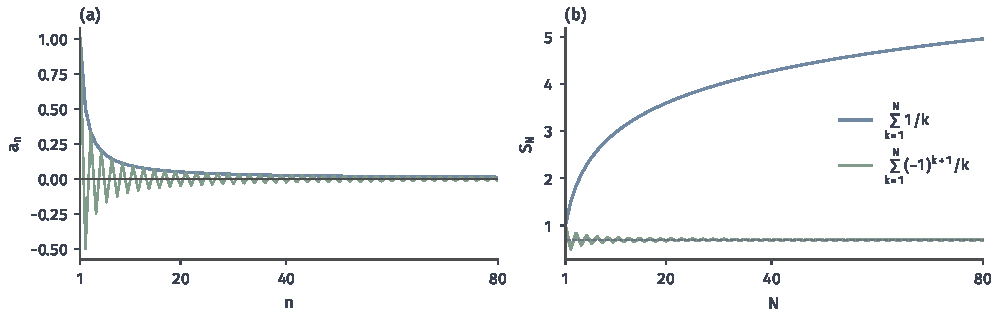
\includegraphics[width=169.0mm]{figures/00-shared/mathematical-preliminaries-upper/00-shared/matplotlib/chapter3-concept-processes/series-terms-sums.pdf}
 \caption{(a) 蓝、绿折线分别连接$1/n$与$(-1)^{n+1}/n$的前80项。(b) 对应的部分和：调和部分和继续增长，交错调和部分和趋于虚线所示的$\log2$。项趋零只是级数收敛的必要条件；图展示有限段，收敛或发散由前面的判别证明。}
 \label{fig:analysis-process-series-terms-sums}
\end{figure*}

\subsection{级数的重排和分组对收敛的影响}
\label{sec:analysis-series-rearrangement-grouping}

收敛判别处理的是原次序下的部分和。接下来改变求和的组织方式：重排改变各项的次序，
分组只把原次序中的有限个相邻项合并；两种操作对收敛性的影响不同，需要分别检验。

\paragraph{级数的重排}
有限和可以交换项的先后；无穷级数则要检查新的部分和如何覆盖旧项。
若$\pi:\{1,2,\ldots\}\to\{1,2,\ldots\}$为双射，$\sum_{n=1}^{\infty}a_{\pi(n)}$称为原级数的重排，
它每项恰好使用一次，改变的是各项进入累计的顺序。

对于非负项，重排的每个部分和只含有限个原下标，这些下标都不超过某个$N$，所以它不超过$s_N$，从而不超过原扩展总和；
反过来，原来的任意前$N$项也会全部进入重排的某个有限前段。对两个方向分别取上确界，便知重排保持总和，允许总和为$+\infty$。

绝对收敛也保证任意重排保持原和。设原级数和为$s$，记重排的部分和为$t_K=\sum_{n=1}^{K}a_{\pi(n)}$。
给定$\varepsilon>0$，先选$N$使$\sum_{n>N}|a_n|<\varepsilon$，再选$K_0$使$\pi(1),\ldots,\pi(K_0)$已包含$1,\ldots,N$。
当$K\geq K_0$时，$t_K-s_N$是若干个下标大于$N$的项之和，故$|t_K-s_N|\leq\sum_{n>N}|a_n|<\varepsilon$；
又由前面的截断误差界，$|s_N-s|<\varepsilon$。因此$|t_K-s|<2\varepsilon$，重排仍收敛到$s$。

条件收敛没有这一保证。记$P_N$、$Q_N$分别为前$N$项中正项之和与负项绝对值之和，
$P$、$Q$为相应的扩展总和。若其中一个有限，由$s_N=P_N-Q_N$收敛会推出另一个也有限，
于是$\sum|a_n|=P+Q$有限，与条件收敛矛盾，故二者都为$+\infty$。

对任意实数目标$L$，可以按原先的相对次序取正项，直到部分和超过$L$，
再取负项直到低于$L$，如此反复；每次都至少取一项相应符号的项。
由于$P=Q=+\infty$，每一轮都会在有限步内结束，两类项最终都被用到；
而$a_n\to0$使每次越过$L$的幅度趋零，因此得到和为$L$的重排。
原级数若含零项，每轮再按原次序插入下一个尚未使用的零项（若有）；这不改变和，并保证每个零项也最终被用到。
也可交替超过$1$、低于$0$，构造不收敛的重排。
可见条件收敛级数的和依赖抵消的顺序，不能按有限和的交换律任意调换。

\paragraph{级数的分组}
分组保持原项的顺序，只将有限个相邻项合为一项。
准确地说，取$0=n_0<n_1<n_2<\cdots$，令
$b_j=\sum_{k=n_{j-1}+1}^{n_j}a_k$，则分组后前$J$项的和恰为$s_{n_J}$。
所以原级数收敛到$s$时，分组后的部分和是原部分和的子序列，也必收敛到$s$；
这对绝对收敛和条件收敛都成立。

反向不成立。级数$1-1+1-1+\cdots$的部分和在$1$与$0$之间交替，原级数不收敛，
但按$(1-1)+(1-1)+\cdots$分组后各项为零。
分组只保留部分截断位置，可能掩盖块内的振荡。

非负项没有这种抵消：原部分和单调，分组截断又越过每一个原截断位置，
两者的上确界相同，故即使总和为$+\infty$也可保序分组。
结合非负项的重排规则，可先把非负项按任意编号排列，再分成有限相邻块，而不改变扩展总和；
后面构造外测度时，将用这些求和性质累计覆盖区间的长度。

\FloatBarrier

\section{函数的极限}
\label{sec:analysis-function-limits}

数列的指标按自然数逐项增加，函数的输入却可以从许多实数位置靠近同一点。例如$(x^2-1)/(x-1)$在$x=1$没有定义，但在$x\neq1$时它等于$x+1$，所以邻近输入的输出仍趋于$2$。函数极限研究的正是这种去掉中心点后的共同趋近，不要求函数在中心有取值。

\subsection{函数极限的定义}
\paragraph{聚点}

讨论输入接近$a$之前，须保证定义域中确实有不同于$a$的输入能够任意靠近$a$。
设$X\subseteq\mathbb R$。若每个$r>0$都能找到$x\in X$使$0<|x-a|<r$，
即$(a-r,a+r)$去掉$a$以后（称为$a$的去心邻域）总含有$X$中的点，就称$a$为$X$的\term{聚点}（cluster point）。
例如$0$是$(0,1)$的聚点，虽然$0$不属于这个集合。
$X$中不是聚点的点称为$X$的\term{孤立点}（isolated point），例如整数集合中的每个点；
在孤立点附近没有其他输入，谈不上“趋近”。

\paragraph{函数极限}
有了能够趋近的输入，还要用输入误差控制输出误差，这与数列极限比较尾部误差的思路相同。
设$f:X\to\mathbb R$，$a$为$X$的聚点，$b\in\mathbb R$。
若对每个$\varepsilon>0$，都存在$\delta>0$使
\[
 x\in X,\quad0<|x-a|<\delta\quad\Longrightarrow\quad|f(x)-b|<\varepsilon,
\]
就称$b$为$x\to a$时$f(x)$的极限，记作$\lim_{x\to a}f(x)=b$。
也就是说，只要输入与$a$足够近，输出与$b$的距离就能任意小。

定义中的$0<|x-a|$排除了中心点，所以既不要求$f(a)$有定义，也不要求它等于$b$。
回到开头的例子$f(x)=(x^2-1)/(x-1)$：对$x\neq1$有$f(x)=x+1$。
给定$\varepsilon>0$，取$\delta=\varepsilon$，则
$0<|x-1|<\delta$时$|f(x)-2|=|x-1|<\varepsilon$，所以其极限为$2$。

图~\ref{fig:analysis-process-epsilon-delta-band}将输入邻域与输出误差带对应起来，同时把基点取值与趋近时的极限分开。
\begin{figure}[!htbp]
 \centering
 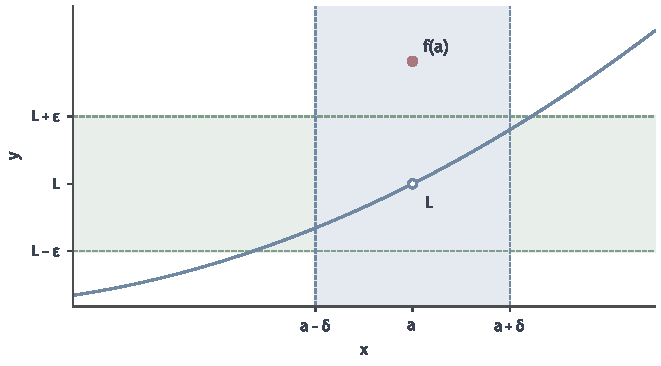
\includegraphics[width=112.0mm]{figures/00-shared/mathematical-preliminaries-upper/00-shared/matplotlib/chapter3-concept-processes/epsilon-delta-band.pdf}
 \caption{取$a=L=1$（$L$即正文中的极限值$b$），$x\neq1$时$f(x)=x^2$，另令$f(1)=2$。蓝带对应$\delta=0.2$的输入范围，绿带对应$\varepsilon=0.55$的输出范围；去掉$a$后，蓝带内曲线全部落在绿带内。空心点是极限位置，红实心点是$f(a)$，不参加去心邻域条件。}
 \label{fig:analysis-process-epsilon-delta-band}
\end{figure}

\paragraph{左极限与右极限}
实轴上的输入可以从一个点的两侧接近，而两侧的输出未必有相同趋向，因此先分别考察每一侧的极限。
只让$x<a$的点趋近$a$，得到左极限$\lim_{x\uparrow a}f(x)$；
只让$x>a$的点趋近$a$，得到右极限$\lim_{x\downarrow a}f(x)$。
两种定义分别在上述误差条件中增加$x<a$或$x>a$，
并要求相应一侧存在定义域中的点任意靠近$a$。
若两侧都能趋近$a$，双侧极限存在当且仅当左右极限都存在且相等。

例如$f(x)=\mathbb I\{x\geq0\}$在$0$处的左右极限分别为$0$和$1$，所以双侧极限不存在。
这里$\mathbb I$为指示函数：括号内条件成立时取$1$，否则取$0$。
在定义域$[a,b]$内，只能从右侧趋近左端点$a$，从左侧趋近右端点$b$。
这种左右判据依赖实轴上的顺序，多元函数还须控制其他趋近方式。

\paragraph{无穷远处的极限}
输入也可以趋于无穷。设定义域向右无界，条件
\[
 \lim_{x\to+\infty}f(x)=b
\]
表示：对每个$\varepsilon>0$，存在$M$，使定义域中所有$x>M$都满足$|f(x)-b|<\varepsilon$。
定义域向左无界时，$x\to-\infty$的定义相应要求所有$x<M$的允许输入满足同一误差界。
例如$1/x$在$x\to+\infty$和$x\to-\infty$时都趋于$0$。

\paragraph{值为无穷的极限}
前一段改变的是输入的趋向；即使输入趋近有限点，输出也可能越过任何有限界，因此还需要描述输出本身的无界趋向。
对有限聚点$a$，$f(x)\to+\infty$（$x\to a$）是指：对每个实数$M$，都存在$\delta>0$，使定义域中满足$0<|x-a|<\delta$的每个$x$都有$f(x)>M$。
趋于$-\infty$则把最后的不等式改为$f(x)<M$。单侧无穷极限再限制输入所在的一侧。
因此$1/x$在$x\downarrow0$时趋于$+\infty$，在$x\uparrow0$时趋于$-\infty$，并没有共同的双侧无穷极限。

\subsection{常见函数的极限}

\paragraph{三角函数}
三角函数的自变量采用弧度制：单位圆上弧长为$h$的圆心角记为$h$。
比较内接三角形、扇形和外切三角形的面积，可得$0<h<\pi/2$时
$\sin h\leq h\leq\tan h$，从而$\cos h\leq\sin h/h\leq1$。
又由$1-\cos h=2\sin^2(h/2)\leq h^2/2$得到误差界
\[
 0\leq1-\frac{\sin h}{h}\leq1-\cos h\leq\frac{h^2}{2}.
\]

任给$\varepsilon>0$，只要$0<h<\min\{\pi/2,\sqrt{2\varepsilon}\}$，第一个比值与$1$的误差就小于$\varepsilon$；
$\sin h/h$是偶函数，所以同一估计也控制$h<0$的一侧。
第二个比值由$|1-\cos h|/|h|\leq|h|/2$控制，这个误差界对正负两侧都适用。因此
\[
 \lim_{h\to0}\frac{\sin h}{h}=1,
 \qquad
 \lim_{h\to0}\frac{\cos h-1}{h}=0.
\]
弧度制使第一个极限恰为$1$，用角度制时会多出比例系数。

\paragraph{自然指数函数}
后面求指数函数的导数需要一个原点处的基本极限。下面先用级数构造自然指数函数并验证其收敛，
再建立乘法性质和局部变化关系。定义
\[
 \exp x=\sum_{k=0}^{\infty}\frac{x^k}{k!}.
\]
对固定$x$，相邻项绝对值之比为$|x|/(k+1)$，当$k+1\geq2|x|$时不超过$1/2$，
尾部被几何级数控制，所以级数绝对收敛。

为得到乘法性质，先考察两个绝对收敛级数$\sum_k a_k$与$\sum_j b_j$的乘积。有限的正方形和满足
$\sum_{k=0}^N\sum_{j=0}^Na_kb_j=(\sum_{k=0}^Na_k)(\sum_{j=0}^Nb_j)$，
所以它们趋于两级数和的乘积。按总次数$k+j=n$合并的三角形部分和$\sum_{n=0}^{N}\sum_{k+j=n}a_kb_j$，
与正方形和只差满足$k,j\leq N$、$k+j>N$的项；这些项的$k$或$j$大于$N/2$，其绝对值之和不超过
$(\sum_{k>N/2}|a_k|)(\sum_j|b_j|)+(\sum_k|a_k|)(\sum_{j>N/2}|b_j|)$，它随$N$增大趋于零。
因此按总次数合并后也得到同一极限。

把这个结论用于指数级数，记
$C_n=\sum_{k=0}^n x^ky^{n-k}/[k!(n-k)!]$。将系数$n$拆为$k+(n-k)$，并分别换一次有限求和的索引，得到
\[
 nC_n=(x+y)C_{n-1},\qquad n\geq1.
\]
由$C_0=1$逐步得到$C_n=(x+y)^n/n!$，因而
\[
 \exp x\,\exp y
 =\sum_{n=0}^{\infty}\sum_{k=0}^n\frac{x^ky^{n-k}}{k!(n-k)!}
 =\sum_{n=0}^{\infty}\frac{(x+y)^n}{n!}
 =\exp(x+y).
\]
记$e=\exp1$，$e$约为$2.71828$。由加法公式，对正整数$n$有$\exp n=e^n$，
因此通常把$\exp x$写作$e^x$，称为以$e$为底的指数函数。

当$0<|h|<1/2$时，利用$1/k!\leq1$直接估计级数的二阶以后各项：
\[
 |e^h-1-h|
 \leq\sum_{k=2}^{\infty}|h|^k
 =\frac{h^2}{1-|h|}\leq2h^2.
\]
除以$|h|$得$|(e^h-1)/h-1|\leq2|h|$，令$h\to0$，就有
\[
 \lim_{h\to0}\frac{e^h-1}{h}=1.
\]
这一推导只用到级数，未使用求导或积分。

加法公式还给出其他性质。由$e^xe^{-x}=e^0=1$知$e^x\neq0$，又$e^x=(e^{x/2})^2\geq0$，因此$e^x>0$。
对$u\geq0$，级数各项非负，只保留前两项便得
\[
 e^u\geq1+u\qquad(u\geq0),
\]
这一不等式给出指数函数在非负半轴上的一个线性下界。
对$h>0$，由此$e^h\geq1+h>1$，于是$e^{x+h}=e^xe^h>e^x$，指数函数严格递增。
同一估计说明$x\to+\infty$时$e^x\to+\infty$；由$e^x=1/e^{-x}$又得$x\to-\infty$时$e^x\to0$。
对固定$x$和$|h|<1/2$，上述余项界还给出$|e^{x+h}-e^x|=e^x|e^h-1|\leq e^x(|h|+2h^2)\to0$。
这些性质将在连续函数的介值定理建立后，用于构造自然对数这一反函数
\scite{math-lebl-analysis1}。

\subsection{函数极限的性质与运算}
\paragraph{序列判据}

函数极限要求控制$a$附近所有允许的输入。这个条件等价于：每列满足$x_n\in X\setminus\{a\}$且$x_n\to a$的输入，都有$f(x_n)\to b$。

正向，给定$\varepsilon$后取函数极限中的$\delta$，充分靠后的$x_n$满足$0<|x_n-a|<\delta$，于是$|f(x_n)-b|<\varepsilon$。
反向用反证法。若误差条件不成立，就存在$\varepsilon_0>0$，使每个$1/n$去心邻域内都能选到$x_n\in X$，满足$|f(x_n)-b|\geq\varepsilon_0$；
这列输入趋于$a$，输出却不趋于$b$，与序列条件矛盾。

\paragraph{和的极限}
序列判据把函数极限转化为数列极限，从而可以逐项借用数列极限的运算法则。
以下各段统一设$f,g:D\to\mathbb R$，$a$为$D$的聚点，且在$x\in D$、$x\to a$时
$f(x)\to b$、$g(x)\to c$，其中$b,c\in\mathbb R$。和的极限为
\[
 \lim_{x\to a}(f(x)+g(x))=b+c.
\]
任取$x_n\in D\setminus\{a\}$且$x_n\to a$，序列判据给出$f(x_n)\to b$、$g(x_n)\to c$；
数列和的法则给出$f(x_n)+g(x_n)\to b+c$。由于对任意这样的输入列都成立，再用序列判据即得结论。

\paragraph{差的极限}
相减也保留有限极限关系：
\[
 \lim_{x\to a}(f(x)-g(x))=b-c.
\]
对每列趋于$a$的允许输入，数列差的法则都给出相应输出差趋于$b-c$，再由序列判据返回函数极限。

\paragraph{数乘的极限}
固定倍数只按比例改变输出误差。对任意固定$\lambda\in\mathbb R$，
\[
 \lim_{x\to a}\lambda f(x)=\lambda b.
\]
沿任意允许输入列使用数列常数倍的极限，再用序列判据即可；$\lambda=0$时输出恒为零。

\paragraph{积的极限}
两个有限极限也可以分别相乘：
\[
 \lim_{x\to a}f(x)g(x)=bc.
\]
沿任意允许输入列应用数列乘积的法则，得到输出积趋于$bc$；序列判据保证这控制了$a$附近的全部允许输入。

\paragraph{商的极限}
商需要额外要求分母极限$c\neq0$，此时
\[
 \lim_{x\to a}\frac{f(x)}{g(x)}=\frac bc.
\]
先取输出误差$|c|/2$，便知$a$的某个去心邻域内有$|g(x)|>|c|/2>0$，商在那里有定义。
在这一邻域内，任意输入列都可使用数列的商法则，再由序列判据得到结论。

若分子分母都趋于零，就不能套用此式。例如$(x^2-1)/(x-1)$在$x\to1$时须先约去公因子$x-1$，才能求出极限$2$。
同样，$\infty-\infty$等形式也须先变形或另外估计。

\paragraph{夹逼定理}
不易直接分解的函数，可以用同趋向的两侧函数控制。设在$a$的某个去心邻域内，所有允许输入满足
$u(x)\leq h(x)\leq v(x)$，且$u(x)\to L$、$v(x)\to L$，其中$L\in\mathbb R$，则
\[
 \lim_{x\to a}h(x)=L.
\]
任给$\varepsilon>0$，取一个共同的去心邻域，使其中$u(x)$和$v(x)$都落在$(L-\varepsilon,L+\varepsilon)$内，
夹在中间的$h(x)$也在其中。例如$-|x|\leq x\sin(1/x)\leq|x|$在$x\neq0$时成立，因此$x\to0$时$x\sin(1/x)\to0$。

\subsection{无穷小与无穷大}

\paragraph{无穷小}
趋向零的量可以出现在数列、函数或后面的微分余项中，先给这类趋向一个统一名称。
在指定的趋向下，极限为$0$的函数（或数列）称为无穷小（infinitesimal）。
例如$x\to0$时，$x$和$x^2$都是无穷小；$n\to\infty$时，$1/n$也是无穷小。
“无穷小”描述变化过程中的极限性质，不是某个固定的很小的非零数。

\paragraph{无穷大}
函数值的绝对值也可能最终超过任意固定门槛，这种趋向与趋零可以通过倒数联系起来。
在指定的趋向下，若$|f(x)|\to+\infty$，则称$f$为无穷大。
例如$x\to0$时，$1/x$为无穷大，但它没有共同的正或负无穷极限。
若$f$在所考察的趋向附近非零，则$|f|\to+\infty$等价于$1/f\to0$。

\paragraph{渐近记号}
\label{sec:comb-growth-scales}
两个函数即使同为无穷小，趋零的相对速度也可以不同。
设在所讨论的趋向附近$g\neq0$，定义
\[
 f=o(g)\quad\text{表示}\quad \frac{f}{g}\longrightarrow0.
\]
这个小$o$记号表示$f$相对于$g$可以忽略。
若$|f/g|$在趋向附近有界，则记$f=O(g)$，称为大$O$记号。
大$O$只要求有常数$C$使$|f|\leq C|g|$最终成立，小$o$则要求这个相对比例趋于零。
例如$x\to0$时$x^2=o(x)$，而$3x=O(x)$但不是$o(x)$。
若$f/g\to1$，还记$f\sim g$；两者都趋零时，称为等价无穷小。
例如$x\to0$时$x+x^2\sim x$，因为$(x+x^2)/x=1+x\to1$。

同样的记号可用于$n\to\infty$的数列：
$3n+7=O(n)$、$n/10=O(n)$，但这两个比值分别趋于$3$和$0.1$，所以都不是$o(n)$；
$10\sqrt n=o(n)$，因为$10\sqrt n/n=10/\sqrt n\to0$。
图~\ref{fig:vol1-add-asymptotic-ratios}画出这三个比值。

\begin{figure}[!htb]
  \centering
  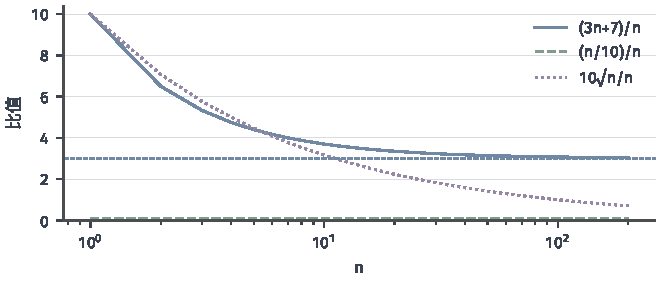
\includegraphics[width=112mm]{figures/00-shared/mathematical-preliminaries-upper/00-shared/matplotlib/mathematical-language-combinatorics-analysis-optimization-comprehension-additions/asymptotic-ratios.pdf}
  \caption{三个解析数列除以$n$后的比值，展示整数$n=1,\ldots,200$，横轴为对数刻度。蓝、绿、紫线的极限分别为$3,0.1,0$。前两者对应$O(n)$而非$o(n)$，第三者对应$o(n)$；极限由正文中的表达式判断，有限范围曲线只帮助观察。}
  \label{fig:vol1-add-asymptotic-ratios}
\end{figure}

对最终为正的数列，若存在$c>0$使$a_n\geq cb_n$最终成立，记$a_n=\Omega(b_n)$；
同时满足$a_n=O(b_n)$与$a_n=\Omega(b_n)$，记$a_n=\Theta(b_n)$，表示同一数量级。
例如$3n+7=\Theta(n)$。这里的常数不随趋于无穷的$n$改变。
$n=O(n^2)$也成立，因此大$O$给出上界，不一定给出精确的增长阶。
这些记号在求导和局部近似中用来表达余项的大小。

\FloatBarrier

\section{实轴上的邻域与闭区间}
\label{sec:analysis-metric-measurement}
\label{sec:analysis-set-metric}

前几节的极限都在控制距离：$|a_n-a|<\varepsilon$说明第$n$项离极限不远，
$0<|x-a|<\delta$说明输入离中心不远。第~\ref{chap:univariate-differentiation}章与第~\ref{chap:univariate-integration}章研究一元函数的连续性、极值和积分时，还要反复回答三个问题：
“一个点附近”指哪些点；什么样的集合能留住其中点列的极限；
在闭区间每一点附近分别成立的控制，怎样合成对整个区间同时有效的控制。
本节依次用邻域与开闭集、闭集的序列判据和闭区间的有限子覆盖性质回答它们。

\subsection{开球、邻域与开闭集}

\paragraph{开球与邻域}
讨论一个点附近的变化，需要先指定哪些点算作离它足够近。

\begin{definition}[开球与邻域]
\label{def:analysis-open-ball}
设$x\in\mathbb R$，$r>0$。开区间
\[
 B(x,r)=\{y\in\mathbb R:|y-x|<r\}=(x-r,x+r)
\]
称为以$x$为中心、半径为$r$的\term{开球}（open ball）。若集合$V\subseteq\mathbb R$包含某个$B(x,r)$，就称$V$是$x$的\term{邻域}（neighborhood）。
\end{definition}

在实轴上，开球就是以$x$为中心的对称开区间；用“球”这个名称，是为了后面换成平面或空间中的距离时沿用同一说法。
上一节的去心邻域就是从$B(a,r)$中去掉中心$a$。
邻域只要求在$x$周围留出一段余量，本身不必是开区间。例如$[0,1]$是$1/2$的邻域，因为它包含$B(1/2,1/4)$；
它却不是端点$0$的邻域，因为每个$B(0,r)$都含有负数。

\paragraph{开集与闭集}
有了开球，就能检验一个集合是否在其中每个点周围都留有余量；对补集作同样检验，又得到闭集。

\begin{definition}[开集与闭集]
\label{def:analysis-open-closed-sets}
集合$U\subseteq\mathbb R$若对每个$x\in U$都存在$r>0$使$B(x,r)\subseteq U$，就称为\term{开集}（open set）；
集合$F\subseteq\mathbb R$若其补集$\mathbb R\setminus F$为开集，就称为\term{闭集}（closed set）。
\end{definition}

开区间$(a,b)$是开集：对其中的$x$，取$r=\min\{x-a,b-x\}$即可。
闭区间$[a,b]$是闭集，因为补集$(-\infty,a)\cup(b,\infty)$中每一点都能取到不碰到$[a,b]$的小球；
$[a,b]$本身不是开集，端点$a$周围的任何开球都含有区间外的点。

$\mathbb R$与空集既开又闭。“不是开集”也不等于“就是闭集”：例如$[0,1)$在$0$处不开，
它的补集在$1$处也不开，所以$[0,1)$既不开也不闭。

有限个开集的交仍是开集：在交集中的每一点，取各个开集所允许半径中最小的一个即可。
无限多个开集的交未必开，例如$\bigcap_{n\geq1}(-1/n,1/n)=\{0\}$。

\subsection{闭集的序列判据}

闭集由补集定义，使用时却常要问：如果集合中的一列点收敛，它的极限是否也属于这个集合？下面说明这两种说法等价。

\begin{lemma}[闭集的序列判据]
\label{lem:analysis-closed-sequence-criterion}
设$F\subseteq\mathbb R$。$F$是闭集，当且仅当：对每个取值于$F$的数列$(x_n)$，若$x_n\to x$，则$x\in F$。
\end{lemma}
\begin{proof}
设$F$闭。若某个取值于$F$的数列收敛到$x\notin F$，开集$\mathbb R\setminus F$包含某个$B(x,r)$；
收敛要求充分靠后的$x_n$落入这个开球，与$x_n\in F$矛盾。

反之，若$F$不闭，则补集不是开集，存在$x\notin F$，使每个$B(x,r)$都与$F$相交。
为每个$n$选$x_n\in F\cap B(x,1/n)$，便有$x_n\to x\notin F$，违反序列条件。
\end{proof}

例如$(0,1)$中的$1/n$趋于$0$，而$0\notin(0,1)$，所以$(0,1)$不是闭集。
闭与有界是不同的性质：$(0,1)$有界但不闭，$\mathbb R$闭但无界。
二者同时成立时，Bolzano--Weierstrass定理~\ref{thm:analysis-bounded-subsequence}给出收敛子列，
本引理又保证子列的极限仍在集合内；第~\ref{chap:univariate-differentiation}章的极值定理正是由此得到。

\subsection{闭区间的有限子覆盖性质}

\paragraph{开覆盖与有限子覆盖}

研究连续函数时，每一点附近都会得到一个局部控制，但不同点所能保证的范围大小可能不同。
要得到对整个闭区间同时有效的结论，需要从无限多个这样的范围中选出有限个，仍覆盖整个区间。
下面先规定“从一族开集中选出有限部分仍不遗漏”的含义。
\begin{definition}[开覆盖与紧致性]
\label{def:analysis-compactness}
设$K\subseteq\mathbb R$。一族开集的并包含$K$时，称它们为$K$的\term{开覆盖}（open cover）；
从中选出的有限个开集仍覆盖$K$时，称它们构成\term{有限子覆盖}（finite subcover）。
若$K$的每个开覆盖都存在有限子覆盖，则称$K$\term{紧致}（compact）。
\end{definition}
开覆盖本身可以有无限多个成员；有限子覆盖要求从原来的成员中挑选，而不是另换一组集合。

\paragraph{闭区间的紧致性}

闭区间有界，Bolzano--Weierstrass定理给出其中点列的收敛子列；闭区间又是闭集，子列的极限仍在区间内。
下面的证明正是用这两点，排除开覆盖必须用到无限多个成员的情形。
\begin{theorem}[闭区间的有限子覆盖性质]
\label{thm:analysis-interval-finite-subcover}
实轴上的每个闭区间$[a,b]$都是紧致集。
\end{theorem}
\begin{proof}
$a=b$时选择一个包含该点的覆盖成员即可。设$a<b$，并给定$[a,b]$的开覆盖$\mathcal U$。
先证明这组覆盖有一个共同尺度：
\begin{equation}
 \exists r>0,\quad\forall x\in[a,b],\quad\exists U\in\mathcal U,
 \qquad B(x,r)\cap[a,b]\subseteq U.
\label{eq:analysis-cover-uniform-radius}
\end{equation}

若不存在这样的$r$，对每个$n$可选$x_n\in[a,b]$，使
$B(x_n,1/n)\cap[a,b]$不包含于任何一个覆盖成员。
有界数列$(x_n)$有收敛子列$x_{n_k}\to x$，由闭集的序列判据，$x\in[a,b]$。
选$U\in\mathcal U$包含$x$，由开性取$\rho>0$使$B(x,\rho)\subseteq U$。
由于$n_k\geq k$，当$k$足够大时，$|x_{n_k}-x|<\rho/2$且$1/n_k<\rho/2$，
于是$B(x_{n_k},1/n_k)\subseteq B(x,\rho)\subseteq U$，与$x_{n_k}$的选取矛盾。

有了共同半径$r$，把$[a,b]$分成有限个长度小于$r$的闭小区间。
每段任选一个点$x$，整段都落在$B(x,r)\cap[a,b]$内，故可由一个覆盖成员包含。
每段选择一个这样的成员，得到有限子覆盖。
\end{proof}

每个有界闭集$K\subseteq\mathbb R$也有此性质：先把它放入某个$[a,b]$，
再把开集$\mathbb R\setminus K$加入它的任意开覆盖，得到$[a,b]$的开覆盖；应用闭区间结论后删去这一补集，剩下的有限个成员仍覆盖$K$。

图~\ref{fig:analysis-process-finite-open-cover}对照一个闭区间的有限覆盖与一个开区间上无法有限选取的覆盖族。
\begin{figure}[!htbp]
 \centering
 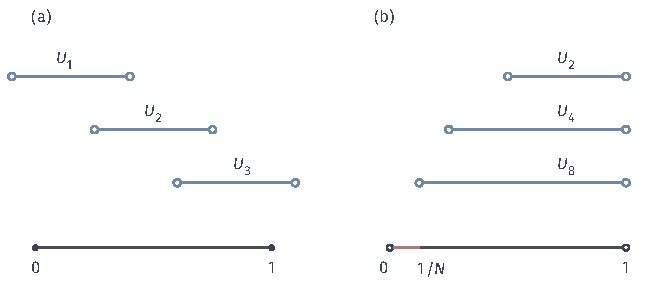
\includegraphics[width=112mm]{figures/00-shared/mathematical-preliminaries-upper/00-shared/tikz/chapter3-concept-processes/finite-open-cover.pdf}
 \caption{(a) 三个开区间$(-0.1,0.4)$、$(0.25,0.75)$、$(0.6,1.1)$覆盖$[0,1]$。(b) $U_n=(1/n,1)$（$n\geq2$）覆盖$(0,1)$；只选有限多个时，设最大下标为$N$，红段$(0,1/N]$仍未覆盖。图只画$U_2,U_4,U_8$；右侧的失败由最大下标论证，不是有限图像的猜测。}
 \label{fig:analysis-process-finite-open-cover}
\end{figure}

以上定义只用到实数之间的距离$|x-y|$。对$\mathbb R^d$中的点$\bm x=(x_1,\ldots,x_d)$与$\bm y=(y_1,\ldots,y_d)$，
把它换成欧氏距离$\lVert\bm x-\bm y\rVert_2=\bigl(\sum_{j=1}^d(x_j-y_j)^2\bigr)^{1/2}$，即各坐标差的平方和再开方
（它满足的三角不等式在第~\ref{sec:ls-norms-distances}节证明），就得到$\mathbb R^d$中的开球$B(\bm x,r)=\{\bm y:\lVert\bm y-\bm x\rVert_2<r\}$、邻域、开集与闭集，
闭集的序列判据连同证明逐字成立；线性空间部分与第~\ref{chap:multivariate-calculus}章使用的正是这些欧氏版本。
欧氏空间中闭有界集的子列性质在第~\ref{chap:multivariate-calculus}章逐坐标证明，一般距离下的开闭集与紧致性在\BookChapterRef{chap:metric-spaces}{第~\ref{chap:metric-spaces}章}讨论。

\FloatBarrier


\FloatBarrier
\section{本章小结}
\label{sec:function-limits-summary}

实值函数可以逐点运算，函数族以整个函数为元素，参数化为它们编号，不同参数可以表示同一个函数；
实数的完备性保证非空有界集合有确界，但函数的下确界未必由某个输入取得，最值是否存在要另行判断。
$|\rho|<1$时等比序列趋于零，有限几何和趋于$1/(1-\rho)$；$|\rho|>1$且$e_0\neq0$时等比序列无界，因而发散。
数列极限先用误差条件规定趋近的含义，再分别研究怎样计算极限、怎样保证极限存在；
单调有界、有界数列的收敛子列与柯西准则都依赖实数的确界原理。
级数把累计过程写成部分和的极限；单项趋零只是必要条件，绝对收敛允许任意重排，
条件收敛的和却依赖次序，而保序分组只保证从原级数的收敛推出分组后的收敛。
函数极限只看去掉中心点后的输入，序列判据把它的运算法则归结为数列情形；渐近记号比较两个量趋零或增长的相对速度。
实轴上的邻域规定局部范围，闭集的序列判据描述极限的归属，
闭区间的紧致性使局部控制能够合成整体控制。

\chapter{一元函数的微分}
\label{chap:univariate-differentiation}
\label{chap:continuous-functions}

设$f:I\to\mathbb R$，其中$I$是实轴上的区间。本章围绕三个问题展开。
第一，输入$x$趋近$a$时，函数值是否趋近$f(a)$？这是连续性的问题。
第二，输入从$a$变到$a+h$时，函数的增量能否近似写成$h$的常数倍？这是可微性的问题。
第三，知道了一点处的变化率，能否据此估计一整段区间上的变化？这要由中值定理和Taylor公式回答。

回答这些问题要用到前面两项准备：第~\ref{sec:analysis-function-limits}节的函数极限描述输入趋近时输出趋向何处，第~\ref{sec:analysis-metric-measurement}节给出了实轴上的邻域、开集、闭集与闭区间的紧致性。

本章先用函数极限定义连续性，比较几种强弱不同的连续性条件，并证明闭有界集上的一致连续性定理；再利用连续性研究闭区间上的最值与介值。
随后用差商的极限定义导数，把它改写为线性近似，推出求导规则。
最后用中值定理和Taylor公式，把一点处的导数信息转化为对有限区间上函数变化的控制。
沿区间累计函数值，以及累计与导数的关系，留给第~\ref{chap:univariate-integration}章。

\section{连续函数}
\label{sec:analysis-local-models}
\label{sec:analysis-metric-continuity-extrema}

\subsection{连续性}

\paragraph{连续函数}
对$f(x)=x^2$，输入$x$接近$a$时，输出$x^2$接近$a^2$，而$a^2$恰好是函数在$a$处的值$f(a)$。连续性描述的就是这种关系：输出趋近的目标等于函数在该点的取值。下面用邻近输入的误差条件表述它；定义域可以是实轴的任意子集，不必是整个区间。
\begin{definition}[连续函数]
\label{def:analysis-continuity}
设$X\subseteq\mathbb R$，$f:X\to\mathbb R$，$a\in X$。若对每个$\varepsilon>0$，都存在$\delta>0$，使
\[
 x\in X,\quad |x-a|<\delta
 \quad\Longrightarrow\quad |f(x)-f(a)|<\varepsilon,
\]
则称$f$在$a$处\term{连续}（continuous）。若$f$在$X$的每一点连续，就称$f$为连续函数。
\end{definition}
定义中的$\delta$可以随$a$和$\varepsilon$改变。连续性与第~\ref{sec:analysis-function-limits}节函数极限的关系，取决于$a$在$X$中的位置。若$a$是$X$的聚点，$x=a$时误差为零，其余输入正是函数极限定义中的去心邻域，所以$f$在$a$处连续等价于$\lim_{x\to a,\,x\in X}f(x)=f(a)$。若$a$是$X$的孤立点，取$\delta$足够小，使邻域内属于$X$的点只有$a$，条件便自动成立。若$X$是闭区间，左端点处只有右侧的输入，连续性就是右极限等于函数值；右端点处相应地使用左极限。

用定义验证连续性时，需要对每个$\varepsilon$具体找出$\delta$。平方函数的验证如下。
\begin{example}[平方函数在每一点连续]
\label{ex:analysis-square-pointwise-continuity}
设$f(x)=x^2$，$x\in\mathbb R$，固定$a\in\mathbb R$。由$x^2-a^2=(x-a)(x+a)$，只需控制因子$|x+a|$。若$|x-a|<1$，则$|x+a|\leq|x-a|+2|a|<2|a|+1$，从而
\[
 |x^2-a^2|\leq(2|a|+1)|x-a|.
\]
给定$\varepsilon>0$，取$\delta=\min\{1,\varepsilon/(2|a|+1)\}$。当$|x-a|<\delta$时，上式给出$|x^2-a^2|<(2|a|+1)\delta\leq\varepsilon$。所以平方函数在每个$a$处连续。
\end{example}
例中所取的$\delta$随$|a|$增大而缩小：基点离原点越远，函数图像越陡，允许的输入误差就越小。第~\ref{sec:analysis-continuity-relations}节将说明，在整条实轴上这种依赖无法消除。

定义~\ref{def:analysis-continuity}只用到实轴上的绝对值距离。把输入与输出的两个绝对值分别换成两个度量空间中的距离，同样的误差条件就定义了一般映射的连续性。这时连续性还取决于所选的距离。例如在实轴上规定不同两点的距离恒为$1$，称为离散距离。恒等映射从离散距离到通常距离是连续的：取$\delta=1/2$，离散距离小于$1/2$的点只有基点本身。反方向却不连续：取$\varepsilon=1/2$，基点的任何通常邻域都含有其他点，它们与基点的离散距离为$1$。

一般度量空间中的连续性、一致连续与Lipschitz条件，以及通常距离与离散距离的对照图，统一在\BookChapterRef{chap:metric-spaces}{第~\ref{chap:metric-spaces}章}建立；本章只使用实轴上的通常距离。

\paragraph{连续性的序列判据}
第~\ref{sec:analysis-function-limits}节用趋近的输入列刻画了函数极限，连续性也有同样的序列刻画；改用序列后，可以直接使用数列极限的结论。具体地，$f:X\to\mathbb R$在$a\in X$处连续，当且仅当对每个满足$x_n\in X$、$x_n\to a$的序列，都有$f(x_n)\to f(a)$。与函数极限的序列判据不同，这里允许某些$x_n$等于$a$，因为$f(a)$本身就是目标值。

若$f$在$a$处连续，任给$\varepsilon>0$，取定义中的$\delta$。序列从某项起满足$|x_n-a|<\delta$，这些项都有$|f(x_n)-f(a)|<\varepsilon$，所以$f(x_n)\to f(a)$。反之，若$f$在$a$处不连续，就存在$\varepsilon_0>0$，使任何$\delta>0$都不满足定义。依次取$\delta=1/n$，可选$x_n\in X$满足$|x_n-a|<1/n$而$|f(x_n)-f(a)|\geq\varepsilon_0$。这列输入趋于$a$，函数值却不趋于$f(a)$，序列条件不成立。

\paragraph{间断点}
若$f$在定义域中的点$a$处不连续，就称$a$为$f$的间断点。按连续性与极限的关系，不连续可能是因为极限存在却不等于函数值，也可能是因为极限根本不存在。下面的可去间断属于前一种情形，跳跃间断则是后一种情形中的一类。

设$a$是定义域的聚点。若$\lim_{x\to a}f(x)$存在且有限，但不等于$f(a)$，就称$a$为可去间断点：把$f(a)$改为这个极限值，函数便在$a$处连续。若左右极限都存在且有限，但两者不相等，就称$a$为跳跃间断点。例如把$x^2$在$0$处的值改为$1$，$0$就成为可去间断点；阶跃函数$\mathbb I\{x\geq0\}$在$0$处的左右极限分别为$0$和$1$，$0$是跳跃间断点。

这两类并未穷尽所有间断情形。例如令$f(0)=0$，$x\neq0$时$f(x)=\sin(1/x)$。沿从右侧趋于$0$的两列点$1/(2\pi n+\pi/2)$与$1/(2\pi n+3\pi/2)$，函数值分别恒为$1$和$-1$，所以右极限不存在；左侧同理。

\subsection{连续函数的运算}

在定义域的聚点处，连续就是极限等于函数值，所以连续函数经过和、差、数乘、积、商运算后是否仍然连续，可以直接由第~\ref{sec:analysis-function-limits}节的函数极限运算法则判断。以下设$f,g:X\to\mathbb R$，$a\in X$是$X$的聚点，极限都沿$X$取。若$a$是$X$的孤立点，任何在$a$处有定义的组合函数都按定义自动在$a$处连续，无需另行讨论。

\paragraph{和的连续性}
若$f,g$在$a$处连续，则$x\to a$时两项分别趋于$f(a)$和$g(a)$。由和的极限法则，
\[
 \lim_{x\to a}(f(x)+g(x))=f(a)+g(a)=(f+g)(a),
\]
所以$f+g$在$a$处连续。

\paragraph{差的连续性}
差的情形相同。若$f,g$在$a$处连续，由差的极限法则，
\[
 \lim_{x\to a}(f(x)-g(x))=f(a)-g(a)=(f-g)(a),
\]
所以$f-g$在$a$处连续。

\paragraph{数乘的连续性}
设$c$为实常数。数乘把输出误差变为原来的$|c|$倍，仍可任意小。若$f$在$a$处连续，由数乘的极限法则，
\[
 \lim_{x\to a}cf(x)=cf(a),
\]
所以$cf$在$a$处连续；$c=0$时$cf$是零函数，同样连续。

\paragraph{积的连续性}
若$f,g$在$a$处连续，两个因子在$a$处都有有限极限，积的极限法则给出
\[
 \lim_{x\to a}f(x)g(x)=f(a)g(a)=(fg)(a),
\]
所以$fg$在$a$处连续。

\paragraph{商的连续性}
商还要求分母在$a$附近不为零。设$f,g$在$a$处连续且$g(a)\neq0$。在$g$的连续性定义中取$\varepsilon=|g(a)|/2$，得到$\delta>0$，使$x\in X$、$|x-a|<\delta$时$|g(x)-g(a)|<|g(a)|/2$，从而$|g(x)|>|g(a)|/2>0$。因此$f/g$在这些输入上有定义，商的极限法则给出
\[
 \lim_{x\to a}\frac{f(x)}{g(x)}=\frac{f(a)}{g(a)},
\]
即$f/g$在$a$处连续。若$g(a)=0$，$f/g$在$a$处没有定义，也就谈不上连续，所以分母非零的条件不能省略。

\paragraph{复合函数的连续性}
复合$g\circ f$要求内层函数的输出能够作为外层函数的输入，因此两层的定义域必须衔接。设$X,Y\subseteq\mathbb R$，$f:X\to Y$在$a\in X$处连续，$g:Y\to\mathbb R$在$f(a)$处连续，则$g\circ f$在$a$处连续。

给定$\varepsilon>0$，先由$g$在$f(a)$处的连续性取$\eta>0$，使$y\in Y$且$|y-f(a)|<\eta$时$|g(y)-g(f(a))|<\varepsilon$；再由$f$在$a$处的连续性取$\delta>0$，使$x\in X$且$|x-a|<\delta$时$|f(x)-f(a)|<\eta$。于是$x\in X$且$|x-a|<\delta$时，$y=f(x)$满足前一条件，从而$|g(f(x))-g(f(a))|<\varepsilon$。这个论证直接使用误差定义，不需要区分聚点与孤立点。

\paragraph{反函数的连续性}
\label{sec:analysis-inverse-continuity}
区间上严格单调的函数把不同输入映成不同输出，因而有反函数；还需说明的是，像点的微小变化只引起反像的微小变化。设$f$在区间$I$上连续且严格单调，则$f$是$I$到像集$f(I)$的一一对应，其反函数$f^{-1}$在$f(I)$上连续。

以严格递增为例。设$a$是$I$的内点，给定$\varepsilon>0$；不妨设$\varepsilon$足够小，使$a-\varepsilon,a+\varepsilon\in I$，因为较小的$\varepsilon$给出更强的结论。严格递增给出$f(a-\varepsilon)<f(a)<f(a+\varepsilon)$。取$\delta=\min\{f(a)-f(a-\varepsilon),\,f(a+\varepsilon)-f(a)\}>0$。若$y\in f(I)$且$|y-f(a)|<\delta$，则$f(a-\varepsilon)<y<f(a+\varepsilon)$；由于$f$严格递增，$f^{-1}(y)$只能落在$a-\varepsilon$与$a+\varepsilon$之间，即$|f^{-1}(y)-a|<\varepsilon$。若$a$是$I$的端点，只在区间内存在的一侧取点，论证相同；严格递减的情形对$-f$讨论即可。

\subsection{连续性条件及其关系}
\label{sec:analysis-continuity-relations}

连续性定义中的$\delta$可以随基点改变，示例~\ref{ex:analysis-square-pointwise-continuity}中平方函数所取的$\delta$就随$|a|$增大而缩小。若要求同一个$\delta$适用于整个定义域，要求输出变化不超过输入变化的固定倍数，或者要求同时控制许多小区间上的总变化，就得到下面几种更强的条件。

\subsubsection{一致连续函数}
一致连续去掉$\delta$对基点的依赖：同一个输入误差界必须对定义域中任意两点同时有效。
\begin{definition}[一致连续函数]
\label{def:analysis-uniform-continuity}
函数$f:X\to\mathbb R$称为\term{一致连续}（uniformly continuous），若对每个$\varepsilon>0$，都存在$\delta>0$，使任意$x,y\in X$满足
\[
 |x-y|<\delta\quad\Longrightarrow\quad |f(x)-f(y)|<\varepsilon.
\]
\end{definition}
这里的$\delta$只依赖$\varepsilon$，不依赖所选的$x,y$。逐点连续的函数未必满足这个更强的要求，平方函数就是一例。
\begin{example}[平方函数在实轴上不一致连续]
\label{ex:analysis-square-not-uniformly-continuous}
设$f(x)=x^2$，$x\in\mathbb R$。取$x_n=n$、$y_n=n+1/n$，则$|y_n-x_n|=1/n\to0$，而
\[
 f(y_n)-f(x_n)=\Bigl(n+\frac1n\Bigr)^2-n^2=2+\frac1{n^2}>2.
\]
假设$f$在$\mathbb R$上一致连续，对$\varepsilon=1$取定义中的$\delta>0$。当$n>1/\delta$时$|y_n-x_n|<\delta$，定义要求$|f(y_n)-f(x_n)|<1$，与上式矛盾。所以平方函数在$\mathbb R$上连续，但不一致连续。
\end{example}
例中的两列点都逃向无穷远：输入越大，平方函数越陡，相同的输入距离造成越大的输出变化，因而找不到对所有位置都适用的$\delta$。

\subsubsection{Lipschitz连续函数}
一致连续只断言共同的$\delta$存在，没有给出输出误差与输入误差的数量关系。若输出距离总不超过输入距离的固定倍数，误差控制就更为具体。
\begin{definition}[Lipschitz连续函数]
\label{def:analysis-lipschitz-continuity}
函数$f:X\to\mathbb R$若存在有限常数$L\geq0$，使所有$x,y\in X$都满足
\begin{equation}
 |f(x)-f(y)|\leq L|x-y|,
\label{eq:analysis-lipschitz-condition}
\end{equation}
则称$f$为\term{Lipschitz连续}（Lipschitz continuous）函数，$L$称为一个Lipschitz常数。
\end{definition}
例如对$x,y\in[0,1]$，$|x^2-y^2|=|x+y|\,|x-y|\leq2|x-y|$，所以平方函数在$[0,1]$上是Lipschitz连续函数，可取$L=2$。Lipschitz条件与其他连续性条件的蕴含关系，留待本节各项定义齐备后在定理~\ref{thm:analysis-continuity-implications}中统一证明。

\subsubsection{局部Lipschitz连续函数}
在整条实轴上，平方函数的割线斜率$(x^2-y^2)/(x-y)=x+y$无界，因此没有适用于全体$x,y$的有限Lipschitz常数；但在每个点附近，$|x+y|$仍然有界。只研究局部变化时，可以让邻域与常数随基点改变。

\begin{definition}[局部Lipschitz连续函数]
\label{def:analysis-local-lipschitz}
设$U\subseteq\mathbb R$为开集，$f:U\to\mathbb R$。若对每个$a\in U$，都存在$r>0$及有限$L\geq0$，使$(a-r,a+r)\subseteq U$，且该区间内的任意$x,y$满足式~\eqref{eq:analysis-lipschitz-condition}，则称$f$为$U$上的\term{局部Lipschitz函数}（locally Lipschitz function）。
\end{definition}
定义中的$r,L$可以随$a$改变。对平方函数，任取$r>0$，区间$(a-r,a+r)$内的$x,y$满足$|x+y|<2(|a|+r)$，故可取$L=2(|a|+r)$。所以平方函数在$\mathbb R$上局部Lipschitz连续，尽管它在整条实轴上不是Lipschitz函数。

\subsubsection{绝对连续函数}
一致连续控制的是单个短区间两端的函数值变化。同时考察有限个互不重叠的小区间时，还可以提出更强的要求：只要这些区间的总长度足够小，各区间端点变化的绝对值之和也足够小。这个要求称为绝对连续。它直接用区间增量定义，不涉及导数或积分。
\begin{definition}[绝对连续函数]
\label{def:measurable-absolutely-continuous-function}
函数$F:[a,b]\to\mathbb R$称为\term{绝对连续函数}（absolutely continuous function），若对每个$\varepsilon>0$都存在$\delta>0$，使任意有限个内部两两不交的子区间$[a_j,b_j]\subseteq[a,b]$满足
\[
 \sum_j(b_j-a_j)<\delta
 \quad\Longrightarrow\quad
 \sum_j|F(b_j)-F(a_j)|<\varepsilon.
\]
\end{definition}
验证绝对连续时，需要同时估计许多小区间上的增量之和。$\sqrt x$在零点附近很陡，可以用来观察这种估计怎样处理陡峭的部分。
\begin{example}[{$\sqrt x$在$[0,1]$上绝对连续}]
\label{ex:analysis-sqrt-absolutely-continuous}
设$F(x)=\sqrt x$，$x\in[0,1]$。给定$\varepsilon>0$，先取$\eta\in(0,1]$使$\sqrt\eta\leq\varepsilon/2$，再取$\delta=\varepsilon\sqrt\eta$。设有限个内部两两不交的子区间$[a_j,b_j]\subseteq[0,1]$满足$\sum_j(b_j-a_j)<\delta$。若某个子区间的内部含有$\eta$，就在$\eta$处把它分成两段；由于$F$递增，该区间上的增量等于两段增量之和，而子区间的总长度不变。分割后，每个子区间都落在$[0,\eta]$或$[\eta,1]$中。

落在$[0,\eta]$中的子区间互不重叠，$F$又递增，所以它们的增量之和不超过整段增量$F(\eta)-F(0)=\sqrt\eta\leq\varepsilon/2$。落在$[\eta,1]$中的每个子区间$[u,v]$满足
\[
 \sqrt v-\sqrt u=\frac{v-u}{\sqrt v+\sqrt u}\leq\frac{v-u}{2\sqrt\eta},
\]
所以这些子区间的增量之和小于$\delta/(2\sqrt\eta)=\varepsilon/2$。两部分合计小于$\varepsilon$，故$\sqrt x$在$[0,1]$上绝对连续。
\end{example}
例中零点附近的割线斜率无界，绝对连续仍然成立：陡峭部分的总增量由$\sqrt\eta$控制，其余部分的割线斜率不超过$1/(2\sqrt\eta)$。

这里的绝对连续约束的是函数在区间上的增量。测度之间也有同名的绝对连续关系，两者的定义对象不同。

至此，连续、一致连续、Lipschitz连续与绝对连续四种条件都已定义，下面比较它们对同一个函数提出的要求。绝对连续只对闭区间上的函数定义，所以四者的比较固定在同一个非退化闭区间上；比较所需的一致连续性定理则可以先对更一般的闭有界集合陈述。

\subsubsection{一致连续性定理}
示例~\ref{ex:analysis-square-not-uniformly-continuous}中的两列点逃向无穷远，逐点连续因而给不出共同的$\delta$。若定义域闭且有界，任何点列都有收敛到定义域内某点的子列，各点的逐点控制就能合并为共同的控制。
\begin{theorem}[闭有界集上的一致连续性定理]
\label{thm:analysis-uniform-continuity}
设$K\subseteq\mathbb R$非空、闭且有界，$f:K\to\mathbb R$连续，则$f$在$K$上一致连续，即
\[
 \forall\varepsilon>0,\quad\exists\delta>0,\quad\forall x,y\in K,\qquad
 |x-y|<\delta\Longrightarrow |f(x)-f(y)|<\varepsilon.
\]
特别地，每个闭区间上的连续函数都一致连续。
\end{theorem}
\begin{proof}
若结论不成立，则存在$\varepsilon_0>0$，使每个$\delta>0$都对应某对$x,y\in K$，满足$|x-y|<\delta$而$|f(x)-f(y)|\geq\varepsilon_0$。
依次取$\delta=1/n$，得到$x_n,y_n\in K$。$K$有界，由Bolzano--Weierstrass定理~\ref{thm:analysis-bounded-subsequence}，可选子列$x_{n_k}\to x$；$K$闭，由闭集的序列判据（引理~\ref{lem:analysis-closed-sequence-criterion}），$x\in K$。
又有$|y_{n_k}-x|\leq|y_{n_k}-x_{n_k}|+|x_{n_k}-x|\to0$，所以$y_{n_k}\to x$。
由$f$在$x$处的连续性，$f(x_{n_k})$与$f(y_{n_k})$都趋于$f(x)$，两者之差趋于零，
与$|f(x_{n_k})-f(y_{n_k})|\geq\varepsilon_0$矛盾。
\end{proof}
定理只用到连续性与定义域的闭有界性，不涉及导数或积分。例如$\sqrt x$在$[0,1]$上连续，因而在$[0,1]$上一致连续。

连续与一致连续是否等价，取决于定义域。图~\ref{fig:analysis-continuity-conditions}(a)(b)画的是同一个平方函数。
(a)对应示例~\ref{ex:analysis-square-not-uniformly-continuous}：实轴闭但无界，不满足定理~\ref{thm:analysis-uniform-continuity}的条件，平方函数连续而不一致连续。
(b)把定义域限制到$[0,1]$，定理保证一致连续；而且$|x^2-y^2|\leq2|x-y|$，平方函数在这里还是Lipschitz常数为$2$的Lipschitz函数。
同一个函数在两个定义域上满足的条件不同，所以比较连续性条件时，必须同时写明函数和定义域。

\subsubsection{闭区间上的蕴含关系}
定义~\ref{def:analysis-continuity}、\ref{def:analysis-uniform-continuity}、\ref{def:analysis-lipschitz-continuity}与\ref{def:measurable-absolutely-continuous-function}分别要求逐点控制、全域共同的误差尺度、线性误差界，以及许多短区间上的总变化受控。在同一个闭区间上，这四种条件有如下强弱关系。
\begin{theorem}[闭区间上连续性条件的关系]
\label{thm:analysis-continuity-implications}
设$a<b$，$f:[a,b]\to\mathbb R$。对同一个$f$和同一个定义域，有
\[
 \text{Lipschitz连续}\ \Longrightarrow\ \text{绝对连续}
 \ \Longrightarrow\ \text{一致连续}\ \Longleftrightarrow\ \text{连续}.
\]
前两个箭头的逆向一般不成立。末尾的等价使用了定义域为闭有界区间的条件。
\end{theorem}
\begin{proof}
若$f$有Lipschitz常数$L$，对任意有限个内部两两不交的子区间，有
\[
 \sum_j|f(b_j)-f(a_j)|\leq L\sum_j(b_j-a_j).
\]
$L>0$时，只要总长度小于$\varepsilon/L$，增量之和就小于$\varepsilon$，满足绝对连续的要求；$L=0$时$f$为常数，增量之和恒为零。

若$f$绝对连续，对给定的$\varepsilon$取定义中的$\delta$，并在定义中只取一个子区间，就得到：任意$x<y$只要满足$y-x<\delta$，便有$|f(y)-f(x)|<\varepsilon$。这正是一致连续。

一致连续的同一个$\delta$适用于每个固定基点，所以一致连续推出连续；反向由闭有界集上的一致连续性定理~\ref{thm:analysis-uniform-continuity}保证。
\end{proof}
两个逆向不成立的例子对应图~\ref{fig:analysis-continuity-conditions}(c)(d)。(c)中的$\sqrt x$说明绝对连续不能推出Lipschitz连续。
\begin{example}[$\sqrt x$绝对连续但不是Lipschitz函数]
\label{ex:analysis-sqrt-not-lipschitz}
示例~\ref{ex:analysis-sqrt-absolutely-continuous}已经证明$\sqrt x$在$[0,1]$上绝对连续。假设它有Lipschitz常数$L$，取$y=0$，则所有$x\in(0,1]$都满足$\sqrt x\leq Lx$，即$1/\sqrt x\leq L$。可是$x\downarrow0$时$1/\sqrt x\to+\infty$，不存在这样的有限常数。所以$\sqrt x$在$[0,1]$上不是Lipschitz函数：从原点出发的割线斜率$1/\sqrt x$无界。
\end{example}
(d)中的康托尔函数说明一致连续不能推出绝对连续：它在$[0,1]$上一致连续，但存在一列区间族，总长度趋于零，端点变化之和却恒为$1$。它的构造与证明见第~\ref{sec:analysis-cantor-function}节。图中的八级折线只是近似，每条有限折线本身都是Lipschitz函数，不能代替证明。

两个例子各自分开了一对相邻的条件：$\sqrt x$表明，控制许多短区间上的总变化弱于线性误差界；康托尔函数表明，控制每个短区间上的变化弱于控制许多短区间上的总变化。
绝对连续的作用要到第~\ref{chap:univariate-integration}章的微积分基本定理才完全显现：它恰好保证函数可以由可积导数恢复。
\begin{figure*}[htbp]
 \centering
 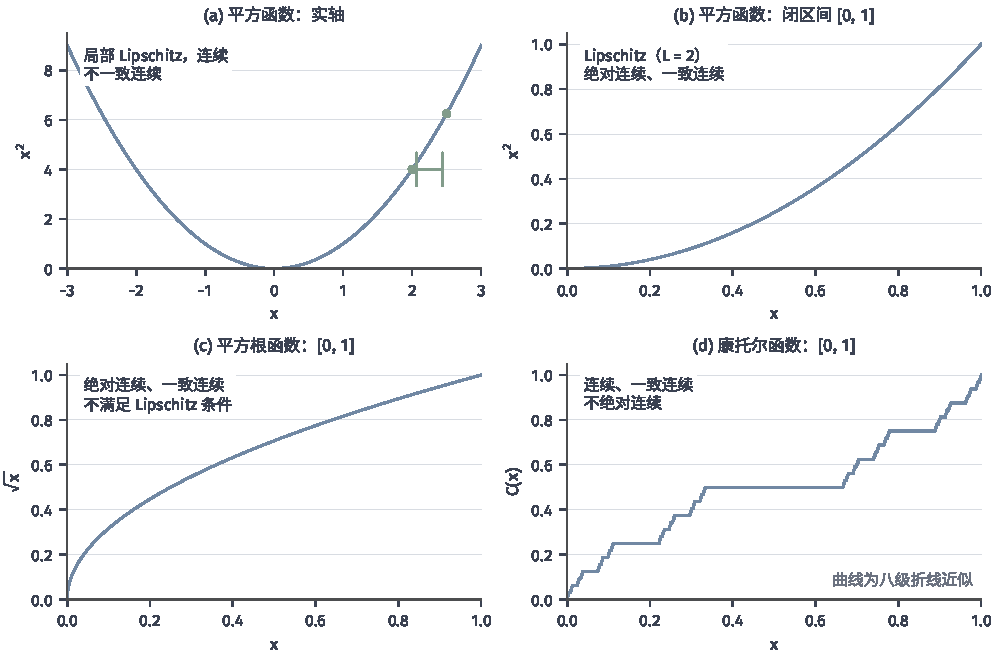
\includegraphics[width=169mm]{figures/00-shared/mathematical-preliminaries-upper/03-calculus/matplotlib/continuity-conditions/figure.pdf}
 \caption{连续性条件依赖于函数和定义域。(a)平方函数在实轴上连续且局部Lipschitz，但不一致连续；只展示$[-3,3]$内的曲线，标记对应$x_2=2$、$y_2=2+1/2$，完整反例使用$x_n=n$、$y_n=n+1/n$两列输入。(b)同一函数限制到$[0,1]$后为Lipschitz函数，因而绝对连续且一致连续。(c)$\sqrt x$在$[0,1]$上绝对连续、一致连续，却不是Lipschitz函数。(d)康托尔函数在$[0,1]$上连续且一致连续，但不绝对连续。右下曲线为八级折线近似，性质标注属于极限函数；每条有限折线本身都是Lipschitz函数，图形不能代替不绝对连续的证明。}
 \label{fig:analysis-continuity-conditions}
\end{figure*}

\subsection{闭区间上连续函数的性质}

\subsubsection{有界性与最值}
第~\ref{sec:prelim-optimal-values-errors}节已经看到，函数的下确界未必能取到，例如$x$在$(0,1)$上没有最小值。所以在寻找最小值之前，需要先知道什么条件保证最值存在。
关键仍是收敛子列：在闭且有界的集合中，Bolzano--Weierstrass定理~\ref{thm:analysis-bounded-subsequence}给出每个序列的收敛子列，
闭集的序列判据（引理~\ref{lem:analysis-closed-sequence-criterion}）保证极限仍在集合内。
再结合连续性，就能证明函数有界并达到最值。
\begin{theorem}[闭有界集上的极值定理]
\label{thm:analysis-extreme-value}
设$K\subseteq\mathbb R$非空、闭且有界，$f:K\to\mathbb R$连续，则$f$有界，且在$K$上达到最小值和最大值。特别地，结论适用于非空闭区间。
\end{theorem}
\begin{proof}
先证有界。若$f$无界，可选$x_n\in K$使$|f(x_n)|>n$。$K$有界，序列$(x_n)$有收敛子列$x_{n_k}\to x$，闭性保证$x\in K$；连续性给出$f(x_{n_k})\to f(x)$。收敛数列有界，这与$|f(x_{n_k})|>n_k\to\infty$矛盾。

再证达到最小值。$f$有界且$K$非空，所以$m=\inf_K f$是有限实数。对每个$n$选$x_n\in K$使$m\leq f(x_n)<m+1/n$。取收敛子列$x_{n_k}\to x^\star\in K$，连续性给出$f(x_{n_k})\to f(x^\star)$；而$f(x_{n_k})$夹在$m$与$m+1/n_k$之间，也趋于$m$，所以$f(x^\star)=m$。对$-f$重复论证即得最大值。
\end{proof}
定理要求定义域闭、定义域有界且函数连续，三个条件缺一不可。下面三个函数各缺少其中一个条件，下确界都取不到。
\begin{example}[极值定理的条件]
\label{ex:analysis-extrema-failures}
定义域不闭：在$(0,1)$上，连续函数$f(x)=x$的下确界为$0$，但$0$不在定义域中，最小值不存在。

定义域无界：实轴闭但无界。$e^x$在$\mathbb R$上连续，$x\to-\infty$时趋于$0$，下确界为$0$；由于$e^x>0$，下确界取不到。

函数不连续：在$[0,1]$上令$f(0)=1$，$x>0$时$f(x)=x$。定义域闭且有界，但$x\downarrow0$时$f(x)\to0\neq f(0)$，$f$在$0$处不连续。下确界仍为$0$，而$f(0)=1$，$x>0$时$f(x)=x>0$，所以最小值不存在。
\end{example}
三个条件分别排除了一种失效方式：有界性保证序列有收敛子列，闭性保证子列的极限仍在定义域内，连续性保证函数值随子列收敛到极限点处的值。

\subsubsection{介值定理}
闭区间上的连续函数还有另一条性质：函数从一个端点值变到另一个端点值时，取遍二者之间的每个数值。
这一结论要求两个端点之间的整段都属于定义域，比极值定理的“闭且有界”更具体。
\begin{theorem}[闭区间上的介值定理]
\label{thm:analysis-intermediate-value}
设$a,b\in\mathbb R$、$a<b$，$f:[a,b]\to\mathbb R$连续。则
\[
 \begin{gathered}
 \forall c\in[\min\{f(a),f(b)\},\max\{f(a),f(b)\}],\\
 \exists\xi\in[a,b],\quad f(\xi)=c.
 \end{gathered}
\]
若$\min\{f(a),f(b)\}<c<\max\{f(a),f(b)\}$，则可取$\xi\in(a,b)$。
\end{theorem}
\begin{proof}
$c=f(a)$或$c=f(b)$时，直接取相应端点。下面设$f(a)<c<f(b)$，令
$S=\{x\in[a,b]:f(x)\leq c\}$。因为$a\in S$且$S$有上界$b$，实数的确界性质给出$u=\sup S\in[a,b]$。
对每个正整数$n$，可选$x_n\in S$满足$u-1/n<x_n\leq u$，于是$x_n\to u$。
连续性使$f(x_n)\to f(u)$，由$f(x_n)\leq c$得到$f(u)\leq c$；又因$f(b)>c$，所以$u\neq b$。
若$f(u)<c$，连续性保证$u$右侧充分近的点仍有函数值小于$c$；
由于$u<b$，可在$[a,b]$内选到这样的点$v>u$。于是$v\in S$，与$u$是$S$的上界矛盾。
因此$f(u)=c$。又因$f(a)<c$，有$u\neq a$，所以$u\in(a,b)$。
若$f(a)>c>f(b)$，对$-f$与$-c$应用同一论证即可。
\end{proof}
定理用到了两个端点之间的整段都属于定义域。定义域闭且有界但有缺口时，介值性可能失效。
\begin{example}[有缺口的定义域上不取中间值]
\label{ex:analysis-intermediate-value-gap}
令$X=[-2,-1]\cup[1,2]$，在$[-2,-1]$上取$f(x)=0$，在$[1,2]$上取$f(x)=1$。对每个$a\in X$取$\delta=1$：若$x\in X$且$|x-a|<1$，则$x$与$a$属于同一段，$f(x)=f(a)$。所以$f$在$X$上连续。$X$闭且有界，$f$在$-2$与$2$处分别取$0$和$1$，却不取中间值$1/2$。
\end{example}
极值定理在这个定义域上仍然成立；闭且有界足以保证最值，却不能代替介值定理中的区间条件。

\par\Needspace{10\baselineskip}
\section{微分的定义}
\label{sec:analysis-derivatives-linear-approximation}

连续性只说明输入接近时函数值也接近，没有说明函数值随输入变化的快慢。本节先用差商的极限定义导数，再把导数改写为函数增量的一阶线性近似，由此定义微分。

\subsection{导数}

\paragraph{差商}
设$f$在包含$a$的某个开区间内有定义。输入从$a$变为$a+h$时，函数增量为$\Delta f=f(a+h)-f(a)$。当$h\neq0$时，比值$\Delta f/h$称为差商，表示这两个输入之间的平均变化率；在图形上，它是连接$(a,f(a))$与$(a+h,f(a+h))$两点的割线斜率。

\paragraph{导数}
让$h$趋于零，两点之间的平均变化率就收缩为一点处的变化率。若差商在$h\to0$时趋于一个有限实数，就定义
\[
 f'(a)=\lim_{h\to0}\frac{f(a+h)-f(a)}h,
\]
称其为$f$在$a$处的\term{导数}（derivative），并称$f$在$a$处可导。导数给出该点的瞬时变化率，在图形上是该点切线的斜率。

若$f$在某个区间内每点都可导，则$a\mapsto f'(a)$又构成一个函数，称为导函数。例如$f(x)=x^2$时，差商$[(a+h)^2-a^2]/h=2a+h$，令$h\to0$得$f'(a)=2a$。

\paragraph{单侧导数}
在区间端点处，或在左右两侧变化方式不同的点处，需要分别考察两侧的差商。
只让$h>0$或只让$h<0$取极限，分别得到右导数$f'_+(a)$和左导数$f'_-(a)$。在内点处，双侧导数存在，当且仅当左右导数都存在、有限且相等。在闭区间端点讨论导数时，本章明确采用从区间内部取得的单侧导数；未特别说明时，内点处的导数都指有限的双侧导数。

\subsection{可微函数}

导数还可以写成函数增量的近似形式。差商趋于$f'(a)$，等价于$f(a+h)-f(a)-f'(a)h$除以$h$后趋于零，即
\begin{equation}
 f(a+h)=f(a)+f'(a)h+o(|h|),\qquad h\to0,
\label{eq:analysis-scalar-first-order}
\end{equation}
其中$o(|h|)$表示除以$|h|$后趋于零的量，沿用第~\ref{sec:comb-growth-scales}节的记号。

式~\eqref{eq:analysis-scalar-first-order}把函数增量分成线性部分$f'(a)h$与高阶余项。反过来，也可以不先假定导数存在，只要求增量有这样的分解：若存在实数$A$，使$h\to0$时$f(a+h)-f(a)=Ah+o(|h|)$，就称$f$在$a$处\term{可微}（differentiable）。两边除以$h$再令$h\to0$，可知差商趋于$A$，所以$f$在$a$处可导且$A=f'(a)$。结合式~\eqref{eq:analysis-scalar-first-order}，一元实函数在内点处可导与可微等价。

可微的分解中，线性部分把输入增量$h$映成函数增量的一阶预测值。线性映射$h\mapsto f'(a)h$称为$f$在$a$处的\term{微分}（differential），记为$\mathrm df_a(h)$。导数$f'(a)$是一个实数，微分则是以它为系数的线性映射。常用记号$\mathrm df=f'(x)\,\mathrm dx$表达同一关系，其中$\mathrm dx$表示输入增量。实际的有限增量$\Delta f$还包含余项，一般不等于微分。

微分与实际增量之差就是式~\eqref{eq:analysis-scalar-first-order}中的余项。用具体数值比较二者，可以看到余项有多大。
\begin{example}[平方函数在$a=3$处的微分]
\label{ex:analysis-square-differential}
设$f(x)=x^2$，$a=3$，则$f'(3)=6$，微分为$\mathrm df_3(h)=6h$。取$h=0.1$，微分给出$0.6$，实际增量为$3.1^2-3^2=0.61$。一般地，
\[
 (3+h)^2-3^2-6h=h^2,
\]
所以两者之差恰为$h^2$，$h=0.1$时为$0.01$。余项$h^2$除以$|h|$后趋于零，符合式~\eqref{eq:analysis-scalar-first-order}。
\end{example}
\begin{example}[$x^3-3x$在$a=1/2$处的一阶近似]
\label{ex:analysis-cubic-linear-approximation}
设$f(x)=x^3-3x$。由$(a+h)^3=a^3+3a^2h+3ah^2+h^3$，差商为$3a^2-3+3ah+h^2$，令$h\to0$得$f'(a)=3a^2-3$。取$a=1/2$，则$f(1/2)=-11/8$、$f'(1/2)=-9/4$，一阶近似为
\begin{equation}
 T_1(\tfrac12+h)=-\frac{11}{8}-\frac94h.
\label{eq:analysis-cubic-linear-model}
\end{equation}
取$h=0.1$，$T_1(0.6)=-1.600$，而$f(0.6)=0.216-1.8=-1.584$，近似值比真值小$0.016$。
\end{example}
第一例的余项恰为$h^2$；第二例余下的$0.016$来自函数图像的弯曲，第~\ref{sec:analysis-second-order-curvature}节将用二阶导数解释它。

可微还蕴含连续。若$f$在$a$处可微，由式~\eqref{eq:analysis-scalar-first-order}，$h\to0$时$f(a+h)-f(a)=f'(a)h+o(|h|)\to0$，即$f$在$a$处连续。

连续却只是可微的必要条件，并不充分。
\begin{example}[绝对值函数在原点连续而不可微]
\label{ex:analysis-absolute-value-not-differentiable}
设$f(x)=|x|$。由$\bigl||x|-|a|\bigr|\leq|x-a|$，$f$在每一点连续。在原点，差商为$|h|/h$：$h>0$时等于$1$，$h<0$时等于$-1$。所以$f'_+(0)=1$、$f'_-(0)=-1$，左右导数不相等，$f$在$0$处不可导，也就不可微。
\end{example}
阶跃函数在原点不连续，由上述必要条件，它在原点也不可微。图~\ref{fig:analysis-continuity-counterexamples}比较了连续且可微、连续但不可微与不连续三种情形。
\begin{figure*}[htbp]
 \centering
 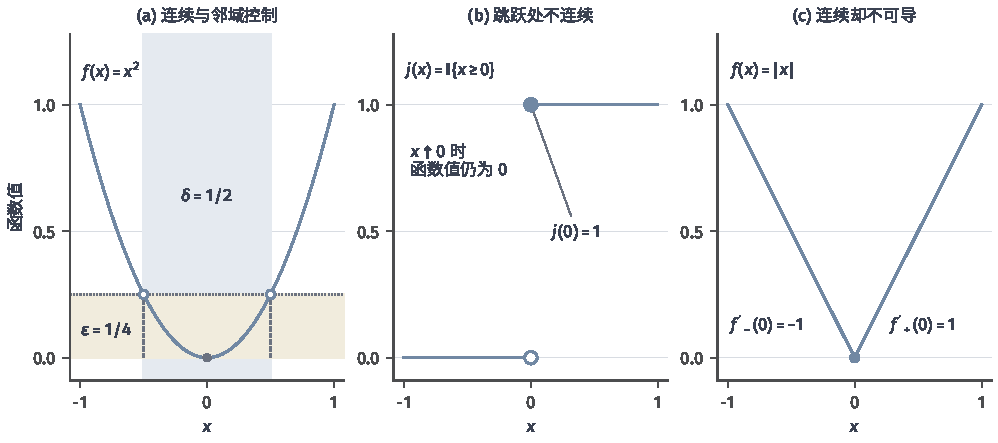
\includegraphics[width=169.0mm]{figures/00-shared/mathematical-preliminaries-upper/03-calculus/matplotlib/analysis-continuity-counterexamples/figure.pdf}
 \caption{平方函数、绝对值函数与阶跃函数在原点的差别。平方函数连续且可微；绝对值函数连续，但左右导数不同；阶跃函数的左右极限不同。连续性控制函数值的极限，可微性还要求差商具有同一个有限极限。}
 \label{fig:analysis-continuity-counterexamples}
\end{figure*}

\subsection{连续可微函数}

可导只要求每一点的差商各自有极限，并不要求邻近位置的导数接近该点的导数。
若进一步要求导函数本身连续，就得到更强的条件：若$f$在开区间$I$上可导且$f'$在$I$上连续，就称$f$连续可微，记为$f\in C^1(I)$。

在闭区间上使用$C^1([a,b])$时，要求$f$在$[a,b]$上连续、在$(a,b)$内可导，且$f'$能连续延拓到两个端点。由后文的Lagrange中值定理（定理~\ref{thm:analysis-lagrange-mean-value}）可以证明，延拓值就是相应的单侧导数。

处处可导与连续可微确实不同：导函数可能在某点不连续。
\begin{example}[处处可导而导函数不连续]
\label{ex:analysis-derivative-not-continuous}
令$f(0)=0$，$x\neq0$时$f(x)=x^2\sin(1/x)$。在原点，差商为$h\sin(1/h)$；由$|h\sin(1/h)|\leq|h|$及夹逼定理，它趋于$0$，所以$f'(0)=0$。在非零点，
\[
 f'(x)=2x\sin\frac1x-\cos\frac1x,
\]
这一公式将在示例~\ref{ex:analysis-oscillating-derivative-formula}中由求导规则得到。取$x_n=1/(2\pi n)$，则$x_n\to0$，而$\sin(1/x_n)=0$、$\cos(1/x_n)=1$，故$f'(x_n)=-1$。$f'(x_n)$不趋于$f'(0)=0$，所以$f'$在$0$处不连续：$f$在$\mathbb R$上处处可导，却不属于$C^1(\mathbb R)$。
\end{example}
导数在原点附近的振荡来自$-\cos(1/x)$一项，它在$-1$与$1$之间反复取值。因此$C^1$是比处处可导更强的条件。

\section{微分的运算法则}
\label{sec:analysis-scalar-chain-rules}

本节由已知函数的导数求组合函数的导数。以下设$f,g$在所讨论的点$a$的某个开邻域内有定义，并在$a$处可导；各条规则都由差商的极限或式~\eqref{eq:analysis-scalar-first-order}的一阶展开得到。

\subsection{四则运算的求导}

\paragraph{和与数乘}
和的差商等于两个差商之和，常数倍的差商等于差商的同一常数倍。令$h\to0$，由极限的和与数乘法则得到$(f+g)'(a)=f'(a)+g'(a)$与$(cf)'(a)=cf'(a)$，其中$c$为实常数。差$f-g=f+(-1)g$的导数由这两条合并得到。

\paragraph{乘积法则}
乘积的增量可以拆成三部分。记$\Delta f=f(a+h)-f(a)$、$\Delta g=g(a+h)-g(a)$，则
\[
 f(a+h)g(a+h)-f(a)g(a)=g(a)\,\Delta f+f(a)\,\Delta g+\Delta f\,\Delta g.
\]
由式~\eqref{eq:analysis-scalar-first-order}，前两项之和为$[f'(a)g(a)+f(a)g'(a)]h+o(|h|)$；两个增量都是$O(|h|)$，它们的乘积属于$O(h^2)$，也是$o(|h|)$。所以$fg$在$a$处可微，一次项的系数就是导数。连同上一段的和法则，得到
\begin{equation}
 \begin{aligned}
 (f+g)'(a)&=f'(a)+g'(a),\\
 (fg)'(a)&=f'(a)g(a)+f(a)g'(a).
 \end{aligned}
\label{eq:analysis-scalar-sum-product-rules}
\end{equation}

\paragraph{商法则}
设$g(a)\neq0$。可导蕴含连续，按商的连续性中的论证，$g$在$a$附近不为零，$f/g$在$a$附近有定义。先求倒数的导数：
\[
 \frac1h\Bigl(\frac1{g(a+h)}-\frac1{g(a)}\Bigr)
 =-\frac{g(a+h)-g(a)}h\cdot\frac1{g(a+h)g(a)}
 \longrightarrow-\frac{g'(a)}{g(a)^2},
\]
其中用到$g(a+h)\to g(a)$。再把$f/g$写成$f\cdot(1/g)$并使用乘积法则，得到
\[
 \left(\frac fg\right)'(a)
 =\frac{f'(a)}{g(a)}-\frac{f(a)g'(a)}{g(a)^2}
 =\frac{f'(a)g(a)-f(a)g'(a)}{g(a)^2}.
\]
条件$g(a)\neq0$既保证$f/g$在$a$附近有定义，也保证公式右侧有意义。

\subsection{复合函数求导}

复合函数的输入变化先经过内层，再传入外层；总的一阶变化由两层的局部变化率共同决定。
若$f$在$a$处可导，$g$在$f(a)$处可导，且$g\circ f$在$a$附近有定义，则
\begin{equation}
 (g\circ f)'(a)=g'(f(a))f'(a).
\label{eq:analysis-scalar-chain-rule}
\end{equation}
这称为\term{链式法则}（chain rule）。

证明时，记$b=f(a)$、$k(h)=f(a+h)-f(a)$。由$f$的一阶展开，$k(h)=f'(a)h+o(|h|)$，所以$k(h)\to0$，并且充分小的$h$满足$|k(h)|\leq(|f'(a)|+1)|h|$。把$g$在$b$处的一阶展开写成
\[
 g(b+k)=g(b)+g'(b)k+|k|\,\varepsilon(k),
\]
其中$k\neq0$时$\varepsilon(k)=[g(b+k)-g(b)-g'(b)k]/|k|$，它在$k\to0$时趋于零，并规定$\varepsilon(0)=0$。代入$k=k(h)$，得到
\[
 g(f(a+h))-g(f(a))=g'(b)f'(a)h+g'(b)\,o(|h|)+|k(h)|\,\varepsilon(k(h)).
\]
最后一项的绝对值不超过$(|f'(a)|+1)|h|\,|\varepsilon(k(h))|$，而$\varepsilon(k(h))\to0$，所以它也是$o(|h|)$。于是$g\circ f$在$a$处可微，一次项系数为$g'(f(a))f'(a)$。规定$\varepsilon(0)=0$使上式在$k(h)=0$时同样成立，所以证明也覆盖$f'(a)=0$等中间增量可能为零的情形，无需除以$k(h)$。

\subsection{反函数求导}
第~\ref{sec:analysis-inverse-continuity}节已经证明，区间上连续且严格单调的函数有连续的反函数。现在判断反函数何时可导，以及它的导数怎样由原函数的导数决定。

设$f:I\to J$在区间$I$上连续且严格单调，$J=f(I)$，其反函数为$g=f^{-1}$。设$a$是$I$的内点，$f$在$a$处可导且$f'(a)\neq0$，记$b=f(a)$。取$r>0$使$a-r,a+r\in I$；由介值定理，$J$包含$f(a-r)$与$f(a+r)$之间的整段，而$b$严格位于二者之间，所以$b$是$J$的内点。对充分小的$k\neq0$，令$h=g(b+k)-a$。$g$是一一对应，所以$h\neq0$；$g$连续，所以$k\to0$时$h\to0$。由$f(a+h)=b+k$，
\[
 \frac{g(b+k)-g(b)}k
 =\frac{h}{f(a+h)-f(a)}\longrightarrow\frac1{f'(a)}.
\]
因此$g$在$b$处可导，且$g'(b)=1/f'(a)$。

对恒等式$f(g(y))=y$使用链式法则，也会得到同一公式；但链式法则要求$g$已经可导，所以上面先用差商证明可导性。公式需要两个条件：$f$在所讨论的区间上一一对应，且在对应点处$f'(a)\neq0$。例如$x^3$在$0$处导数为零，其反函数$\sqrt[3]y$在$0$处的差商为$1/(\sqrt[3]k)^2$，$k\to0$时无界，所以反函数在$0$处不可导。

\subsection{基本初等函数的导数}
\label{sec:analysis-elementary-derivatives}

有了四则运算、复合与反函数的求导规则，复杂函数的求导就归结为少数基本函数的导数。以下逐类从差商推出这些导数，并注明成立范围。

\subsubsection{常数函数与整数幂函数}
常数函数$f(x)=c$的差商恒为零，恒等函数$f(x)=x$的差商恒为$1$，所以二者的导数分别为$0$和$1$。
对正整数$m$，把$x^m$看成$m$个恒等函数的乘积，反复使用乘积法则：每一项只对一个因子求导、保留其余$m-1$个因子，共有$m$项，每项都等于$x^{m-1}$，所以$(x^m)'=mx^{m-1}$。
$m=0$时$x^0=1$是常数函数，公式右侧按$0$理解。

对负整数$m=-n$（$n$为正整数），在$x\neq0$处把$x^m$写成$1/x^n$，由商法则，
\[
 \Bigl(\frac1{x^n}\Bigr)'=-\frac{nx^{n-1}}{x^{2n}}=-nx^{-n-1}=mx^{m-1},
\]
仍是同一形式。于是
\[
 \begin{aligned}
 (c)'&=0,\\
 (x^m)'&=mx^{m-1}\qquad(m\in\mathbb Z),
 \end{aligned}
\]
其中$m\geq0$时对全体实数$x$成立，$m<0$时要求$x\neq0$。

\subsubsection{正弦函数与余弦函数}
三角函数采用弧度制。第~\ref{sec:analysis-function-limits}节已经得到$\sin h/h\to1$与$(\cos h-1)/h\to0$。由正弦、余弦的加法公式，两个差商都能写成这两个比值的组合：
\[
 \begin{aligned}
 \frac{\sin(x+h)-\sin x}{h}
 &=\sin x\frac{\cos h-1}{h}+\cos x\frac{\sin h}{h}
 \longrightarrow\cos x,\\
 \frac{\cos(x+h)-\cos x}{h}
 &=\cos x\frac{\cos h-1}{h}-\sin x\frac{\sin h}{h}
 \longrightarrow-\sin x.
 \end{aligned}
\]
因此
\[
 \begin{aligned}
 (\sin x)'&=\cos x,\\
 (\cos x)'&=-\sin x,
 \end{aligned}
\]
两式对全体实数$x$成立。
若改用角度制，基本极限$\sin h/h$会多出比例系数$\pi/180$，导数公式也随之多出这个系数。

\subsubsection{指数函数}
自然指数函数满足$e^{x+h}=e^xe^h$。由第~\ref{sec:analysis-function-limits}节的基本极限$(e^h-1)/h\to1$，得到
\[
 \frac{e^{x+h}-e^x}{h}=e^x\frac{e^h-1}{h}\longrightarrow e^x.
\]
推导只用到由级数得到的乘法公式和这个基本极限，不依赖其他求导结果。因此
\[
 (e^x)'=e^x\qquad(x\in\mathbb R).
\]

\subsubsection{对数函数与实数幂函数}
自然对数定义为指数函数的反函数，先要确认这个反函数存在。$e^x$连续、严格递增且恒为正，$x\to-\infty$时趋于$0$，$x\to+\infty$时趋于$+\infty$。对任意$y>0$，先选两点使指数值分别小于和大于$y$，再用介值定理得到原像；严格递增保证原像唯一。所以指数函数是$\mathbb R$到$(0,\infty)$的一一对应，其反函数称为自然对数，记为$\log x$（也记$\ln x$），定义在$x>0$上。指数函数的导数$e^x$处处非零，由反函数求导，$(\log x)'=1/e^{\log x}=1/x$。

设$a>0$且$a\neq1$。实数次幂定义为$a^x=e^{x\log a}$，它的反函数$\log_a x$等于$(\log x)/(\log a)$，因为$a^{(\log x)/(\log a)}=e^{\log x}=x$。由链式法则，$(a^x)'=e^{x\log a}\log a=a^x\log a$；由数乘法则，$(\log_a x)'=1/(x\log a)$。
对任意实数$\alpha$，在$x>0$上定义$x^\alpha=e^{\alpha\log x}$，链式法则给出$(x^\alpha)'=e^{\alpha\log x}\cdot\alpha/x=\alpha x^{\alpha-1}$。于是
\[
 \begin{aligned}
 (\log x)'&=\frac1x, &&x>0,\\
 (\log_a x)'&=\frac1{x\log a}, &&x>0,\\
 (x^\alpha)'&=\alpha x^{\alpha-1}, &&x>0,\\
 (a^x)'&=a^x\log a, &&x\in\mathbb R.
 \end{aligned}
\]
这里没有为负数底数定义任意实数次幂，所以$x^\alpha$的公式只在$x>0$上使用。

\subsubsection{基本初等函数导数表}
表~\ref{tab:analysis-elementary-derivatives}汇总了上面得到的公式及成立范围。
把它们与四则运算法则、链式法则和反函数求导结合，就能求出由这些函数经有限次运算与复合得到的初等函数的导数。
示例~\ref{ex:analysis-derivative-not-continuous}在非零点使用的导数公式，就可以这样由乘积法则、链式法则和正弦导数得到。
\begin{example}[$x^2\sin(1/x)$在非零点的导数]
\label{ex:analysis-oscillating-derivative-formula}
设$x\neq0$。内层函数$1/x=x^{-1}$的导数为$-1/x^2$，由链式法则和正弦导数，$\bigl(\sin(1/x)\bigr)'=-\cos(1/x)/x^2$。再由乘积法则，
\[
 \Bigl(x^2\sin\frac1x\Bigr)'
 =2x\sin\frac1x+x^2\Bigl(-\frac1{x^2}\cos\frac1x\Bigr)
 =2x\sin\frac1x-\cos\frac1x.
\]
\end{example}
这些规则不能用于原点，因为$\sin(1/x)$在$0$处没有定义；原点处的导数须直接用差商计算，正如示例~\ref{ex:analysis-derivative-not-continuous}所做。
\begin{table}[htbp]
 \centering\small
 \begin{tabular}{@{}lll@{}}
 \toprule
 函数 & 导数 & 成立范围\\
 \midrule
 $c$ & $0$ & $x\in\mathbb R$\\
 $x^m$（$m\in\mathbb Z$） & $mx^{m-1}$ & $m\geq0$时$x\in\mathbb R$；$m<0$时$x\neq0$\\
 $x^\alpha$（$\alpha\in\mathbb R$） & $\alpha x^{\alpha-1}$ & $x>0$\\
 $\sin x$ & $\cos x$ & $x\in\mathbb R$\\
 $\cos x$ & $-\sin x$ & $x\in\mathbb R$\\
 $e^x$ & $e^x$ & $x\in\mathbb R$\\
 $a^x$（$a>0$，$a\neq1$） & $a^x\log a$ & $x\in\mathbb R$\\
 $\log x$ & $1/x$ & $x>0$\\
 $\log_a x$（$a>0$，$a\neq1$） & $1/(x\log a)$ & $x>0$\\
 \bottomrule
 \end{tabular}
 \caption{基本初等函数的导数。三角函数采用弧度制，$\log$为自然对数。}
 \label{tab:analysis-elementary-derivatives}
\end{table}

\section{闭区间上可微函数的性质}

导数记录一点处的变化率。本节把它与区间上的极值、端点之间的净变化以及两点之间的变化幅度联系起来。
涉及闭区间$[a,b]$的中值结论都只要求函数在$[a,b]$上连续、在$(a,b)$内可导，不要求端点处的单侧导数存在。

\subsection{局部极值与驻点}

\paragraph{局部极值}
导数只反映一点附近的变化，与它对应的是只比较邻近函数值的极值，而不是整个定义域上的最值。
设$c$属于$f$的定义域。若存在$r>0$，使定义域中所有满足$|x-c|<r$的$x$都有$f(x)\geq f(c)$，则称$c$为$f$的局部极小点；若其中$x\neq c$的点都满足严格不等式$f(x)>f(c)$，则称$c$为严格局部极小点。
把不等号反向，就得到局部极大点和严格局部极大点。

\paragraph{Fermat定理}
局部极值比较的是邻近的函数值，导数是差商的极限。在内点处可以从两侧取差商，差商的符号把这两种信息联系起来。
\begin{theorem}[Fermat定理]
\label{thm:analysis-fermat}
设$a<b$，$f:[a,b]\to\mathbb R$，$c\in(a,b)$。若$f$在$c$处可导，且$c$为$f$的局部极小点或局部极大点，则
\begin{equation}
 f'(c)=0.
\label{eq:analysis-scalar-first-order-necessary}
\end{equation}
\end{theorem}
\begin{proof}
设$c$为局部极小点。充分小的$h\neq0$满足$f(c+h)-f(c)\geq0$，
故$h>0$时差商非负，$h<0$时差商非正。
两侧差商趋于同一个有限导数，因而同时有$f'(c)\geq0$与$f'(c)\leq0$，即$f'(c)=0$。
局部极大点对$-f$应用同一论证即可。
\end{proof}
导数为零的点称为\term{驻点}（stationary point）。Fermat定理说明，内点处可导的局部极值点必为驻点。这一必要条件既不能逆用，也不能搬到端点上。
\begin{example}[非极值的驻点与端点处的极值]
\label{ex:analysis-fermat-condition-failures}
设$f(x)=x^3$。由$(x^3)'=3x^2$，$f'(0)=0$，所以$0$是驻点。但$x<0$时$f(x)<0=f(0)$，$x>0$时$f(x)>0=f(0)$；$0$的任何邻域内都有比$f(0)$更小和更大的函数值，所以$0$不是局部极值点。

再设$g(x)=x$，$x\in[0,1]$。$g$在端点$0$处取最小值，但右导数$g'_+(0)=1\neq0$。端点处只能从一侧取差商，Fermat定理证明中两侧差商的符号对比无法进行。
\end{example}
因此Fermat定理只给出内点处极值的必要条件。驻点是否为极值点，还要看函数在它两侧的增减；第~\ref{sec:analysis-monotonicity}节将用导数的符号判断这一点。

\subsection{中值定理}

\subsubsection{Rolle定理}
若函数在区间两端取同一值，整段的净变化为零。
在连续、可导的条件下，区间内部必有一点的瞬时变化率也为零。
\begin{theorem}[Rolle定理]
\label{thm:analysis-rolle}
设$a<b$，$f:[a,b]\to\mathbb R$在$[a,b]$上连续、在$(a,b)$内可导。
若$f(a)=f(b)$，则
\[
 \exists c\in(a,b),\qquad f'(c)=0.
\]
\end{theorem}
\begin{proof}
若$f$恒定，任取$c\in(a,b)$即可。
否则存在$x_0\in(a,b)$使$f(x_0)\neq f(a)$。
由闭区间上的极值定理~\ref{thm:analysis-extreme-value}，$f$在$[a,b]$上达到最大值和最小值。若$f(x_0)>f(a)=f(b)$，最大值不小于$f(x_0)$，严格大于两端的值，所以最大值必在某个内点达到；
若$f(x_0)<f(a)=f(b)$，同理最小值必在某个内点达到。
这个内点是局部极值点，$f$在那里可导，由Fermat定理~\ref{thm:analysis-fermat}，导数为零。
\end{proof}

\subsubsection{Lagrange中值定理}
两端取值不同时，可以先减去连接两个端点的直线，使剩余函数在两端相等，再对它应用Rolle定理。
这样就把整段的平均变化率与某个内点的瞬时变化率联系起来。
\begin{theorem}[Lagrange中值定理]
\label{thm:analysis-lagrange-mean-value}
设$a<b$，$f:[a,b]\to\mathbb R$在$[a,b]$上连续、在$(a,b)$内可导，则存在$c\in(a,b)$使
\begin{equation}
 f(b)-f(a)=f'(c)(b-a).
\label{eq:analysis-mean-value-theorem}
\end{equation}
等价地，$f'(c)=[f(b)-f(a)]/(b-a)$。
\end{theorem}
\begin{proof}
令
\[
 H(x)=f(x)-f(a)-\frac{f(b)-f(a)}{b-a}(x-a).
\]
$H$在$[a,b]$上连续、在$(a,b)$内可导，并满足$H(a)=H(b)=0$。
Rolle定理给出某个$c\in(a,b)$使
$H'(c)=f'(c)-[f(b)-f(a)]/(b-a)=0$，整理即得结论。
\end{proof}
这就是Lagrange\term{中值定理}（mean value theorem）的含义：区间上的平均变化率等于某个内点处的瞬时变化率。
定理只要求函数在每个内点可导，不要求导函数连续。

图~\ref{fig:analysis-process-mean-value-parallel}以$f(x)=x^2$、区间$[0,1]$为例：端点割线的斜率为$1$，$c=1/2$处的切线斜率$f'(1/2)=1$与之相等，两线平行。
\begin{figure}[!htbp]
 \centering
 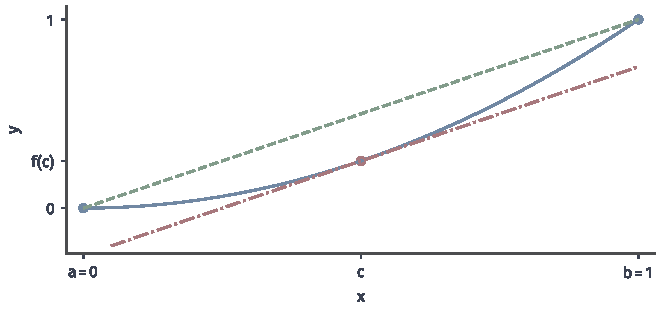
\includegraphics[width=112.0mm]{figures/00-shared/mathematical-preliminaries-upper/00-shared/matplotlib/chapter3-concept-processes/mean-value-parallel.pdf}
 \caption{$f(x)=x^2$在$[0,1]$上，绿虚线为端点割线，红点划线为$c=1/2$处的切线。两线平行，因为$f'(c)=1=[f(1)-f(0)]/(1-0)$。两线高度不同：相等的是斜率，两条直线并不重合。}
 \label{fig:analysis-process-mean-value-parallel}
\end{figure}

\subsubsection{Cauchy中值定理}
比较两个函数在同一区间上的变化时，可以把两者的端点增量放进同一个辅助函数，再应用Rolle定理。
结论先写成交叉相乘的形式，这样不需要假设任何分母非零。
\begin{theorem}[Cauchy中值定理]
\label{thm:analysis-cauchy-mean-value}
设$a<b$，$f,g:[a,b]\to\mathbb R$均在$[a,b]$上连续、在$(a,b)$内可导，则存在$c\in(a,b)$使
\[
 (f(b)-f(a))g'(c)=(g(b)-g(a))f'(c).
\]
若进一步有$g'(x)\neq0$对每个$x\in(a,b)$成立，则$g(b)\neq g(a)$，并可写为
\[
 \frac{f(b)-f(a)}{g(b)-g(a)}=\frac{f'(c)}{g'(c)}.
\]
\end{theorem}
\begin{proof}
令
\[
 \begin{aligned}
 H(x)={}&(f(b)-f(a))(g(x)-g(a))\\
        &-(g(b)-g(a))(f(x)-f(a)).
 \end{aligned}
\]
$H$继承两函数的连续、可导条件，并有$H(a)=H(b)=0$。
应用Rolle定理得$H'(c)=0$，展开导数即为交叉相乘形式。
若$g'$在$(a,b)$内处处非零，$g(b)=g(a)$会使Rolle定理给出某个内点处$g'=0$，产生矛盾，故$g(b)\neq g(a)$。
此时$g'(c)\neq0$，交叉相乘形式两边同除以$(g(b)-g(a))g'(c)$，即得比值形式。
\end{proof}
取$g(x)=x$，则$g'=1$，比值形式就是Lagrange中值定理。

\subsection{单调性}
\label{sec:analysis-monotonicity}

\subsubsection{导数符号与单调性}
中值定理把任意两点之间的函数增量写成某个内点处的导数乘以输入增量，所以导数的符号可以控制整段的增减。
这里的关键是任意两点之间的整段都属于定义域。
\begin{theorem}[导数符号与单调性]
\label{thm:analysis-derivative-monotonicity}
设$a<b$，$f:[a,b]\to\mathbb R$在$[a,b]$上连续、在$(a,b)$内可导。
若$f'(x)\geq0$对所有$x\in(a,b)$成立，则$f$在$[a,b]$上单调不减；若处处有$f'(x)>0$，则严格递增。
相应地，$f'\leq0$蕴含单调不增，$f'<0$蕴含严格递减。
若$f'$在$(a,b)$内恒为零，则$f$在$[a,b]$上为常数。
\end{theorem}
\begin{proof}
任取$a\leq x<y\leq b$，在$[x,y]$上应用Lagrange中值定理，存在$\xi\in(x,y)$使
\[
 f(y)-f(x)=f'(\xi)(y-x).
\]
因为$y-x>0$，右侧的符号由$f'(\xi)$决定，于是得到四种单调性结论。
导数恒为零时，任意两点的函数值都相等，所以函数为常数。
\end{proof}
导数恒为零只保证函数在每个区间上为常数。若定义域由分离的区间组成，各段的常数未必相同：例如在$(0,1)\cup(2,3)$上，左段取$0$、右段取$1$的函数导数处处为零，却不是常数。中值定理不能跨过定义域的缺口使用。

导数为零也不妨碍严格单调：$x^3$在整个实轴上严格递增，因为$x<y$时$y^3-x^3=(y-x)(x^2+xy+y^2)>0$，但它在$0$处导数为零。因此“导数处处严格为正”是严格递增的充分条件，不是必要条件。

\subsubsection{驻点的一阶导数判别}
驻点条件本身不能判定极值，示例~\ref{ex:analysis-fermat-condition-failures}中的$x^3$在驻点$0$两侧都递增。
单调性定理把导数符号转化为增减方向，于是可以比较驻点两侧的变化：先降后升给出极小，先升后降给出极大。
\begin{theorem}[驻点的一阶导数判别]
\label{thm:analysis-first-derivative-test}
设$r>0$，$f$在$[c-r,c+r]$上连续、在$(c-r,c+r)$内可导，且$f'(c)=0$。
若
\[
 f'(x)<0\quad(c-r<x<c),\qquad
 f'(x)>0\quad(c<x<c+r),
\]
则$c$为$f$的严格局部极小点。
若两个区间上的导数符号分别为正和负，则$c$为$f$的严格局部极大点。
\end{theorem}
\begin{proof}
先考虑左负右正的情形。对$c-r<x<c$，$f$在$[x,c]$上连续，且在$(x,c)$内$f'<0$，由定理~\ref{thm:analysis-derivative-monotonicity}，$f$在$[x,c]$上严格递减，故$f(x)>f(c)$；
对$c<x<c+r$，在$[c,x]$上同理得到$f$严格递增，也有$f(x)>f(c)$。
所以$c$两侧充分近的异点都有更大的函数值，$c$为严格局部极小点。
左正右负时反向比较，得到$f(x)<f(c)$，因此$c$为严格局部极大点。
\end{proof}
判别法只需检查导数在驻点两侧的符号。导数能够因式分解时，各因子的符号就给出导数的符号。
\begin{example}[$x^3-3x$的驻点]
\label{ex:analysis-cubic-stationary-points}
设$f(x)=x^3-3x$，则$f'(x)=3x^2-3=3(x-1)(x+1)$，驻点为$x=\pm1$。在定理~\ref{thm:analysis-first-derivative-test}中取$r=1$。

对$x=1$：$0<x<1$时$x-1<0$、$x+1>0$，故$f'(x)<0$；$1<x<2$时两个因子都为正，故$f'(x)>0$。导数由负变正，$1$是严格局部极小点，$f(1)=-2$。

对$x=-1$：$-2<x<-1$时两个因子都为负，故$f'(x)>0$；$-1<x<0$时$x-1<0$、$x+1>0$，故$f'(x)<0$。导数由正变负，$-1$是严格局部极大点，$f(-1)=2$。

$1$只是局部极小点：$x\to-\infty$时$f(x)\to-\infty$，$f$在$\mathbb R$上没有最小值。
\end{example}
若导数在驻点两侧同号，例如$x^3$在$0$两侧都有$f'(x)=3x^2>0$，函数在驻点两侧沿同一方向变化，驻点就不是极值点。

\subsection{Lipschitz条件}

导数的符号控制增减方向；若还能统一限制导数的绝对值，就可以控制任意两点之间的变化幅度。
中值定理把这一导数上界直接转为第~\ref{sec:analysis-continuity-relations}节定义的Lipschitz条件。
\begin{theorem}[有界导数与Lipschitz条件]
\label{thm:analysis-bounded-derivative-lipschitz}
设$a<b$，$f:[a,b]\to\mathbb R$在$[a,b]$上连续、在$(a,b)$内可导。
若存在有限常数$L\geq0$使$|f'(x)|\leq L$对所有$x\in(a,b)$成立，则
\[
 \forall x,y\in[a,b],\qquad |f(y)-f(x)|\leq L|y-x|.
\]
即$f$在$[a,b]$上为Lipschitz连续函数，$L$是一个Lipschitz常数。
\end{theorem}
\begin{proof}
$x=y$时两侧都为零；$x<y$时，Lagrange中值定理给出$\xi\in(x,y)$，使
\[
 |f(y)-f(x)|=|f'(\xi)|\,|y-x|\leq L|y-x|.
\]
$x>y$时交换两点即可。
\end{proof}
例如$f(x)=x^2$在$(0,1)$内有$|f'(x)|=2x\leq2$，所以在$[0,1]$上可取$L=2$，与直接估计$|x^2-y^2|\leq2|x-y|$一致。
定理给出的是Lipschitz条件的充分条件；与单调性定理一样，它要求两点之间的整段都属于定义域。

若$f\in C^1([a,b])$，连续导数在闭区间上有界（极值定理~\ref{thm:analysis-extreme-value}），由上面的定理，$f$是Lipschitz连续函数；再由定理~\ref{thm:analysis-continuity-implications}，$f$绝对连续且一致连续。
反过来，Lipschitz连续不能保证导数处处存在：$|x|$在$[-1,1]$上Lipschitz连续，却在$0$处不可导（示例~\ref{ex:analysis-absolute-value-not-differentiable}）。
因此，函数值变化受控与经典导数处处存在是两种不同的条件，需要分别检查。

\section{高阶微分}

\subsection{高阶导数}

\paragraph{二阶导数}
要研究斜率本身怎样变化，可以继续对导函数求导。
若导函数$f'$在某点可导，它在该点的导数称为$f$的二阶导数，记为$f''$。例如$f(x)=x^3-3x$时，$f'(x)=3x^2-3$，$f''(x)=6x$。

\paragraph{高阶导数}
依次定义$f^{(r)}=(f^{(r-1)})'$，并约定$f^{(0)}=f$。
若$f$在开区间$I$上直到第$r$阶的导数都存在且连续，就称$f$为$r$阶连续可微函数，记为$f\in C^r(I)$，不致混淆时简写为$C^r$。$C^r([a,b])$在端点处的导数采用从内部取得的连续延拓，与$C^1([a,b])$的约定相同。

与一阶微分$\mathrm df=f'(x)\,\mathrm dx$对应，以$x$为自变量时，$r$阶微分记为$\mathrm d^rf=f^{(r)}(x)(\mathrm dx)^r$。它只给出第$r$阶变化的系数；用它近似实际增量时，还需要Taylor公式中的阶乘因子与余项。

\subsection{Taylor公式}
\label{sec:analysis-taylor-approximation}

一阶近似只用到一阶导数。要提高精度，可以依次加入二阶、三阶等高阶项，同时估计截去部分的误差。本节先用一个例子观察二次项补充了什么，再给出一般阶数的Taylor公式及其两种余项。

\subsubsection{二阶近似}
\label{sec:analysis-second-order-curvature}
示例~\ref{ex:analysis-cubic-linear-approximation}中，$x^3-3x$在$1/2$处的一阶近似在$h=0.1$时比真值小$0.016$。一阶近似只用了函数值和斜率；加入由二阶导数确定的二次项，可以看出这部分误差的来源。
\begin{example}[$x^3-3x$在$a=1/2$处的二阶近似]
\label{ex:analysis-cubic-quadratic-approximation}
仍设$f(x)=x^3-3x$。由$f''(x)=6x$，得$f''(1/2)=3$。在式~\eqref{eq:analysis-cubic-linear-model}上加入二次项$\tfrac12f''(1/2)h^2=\tfrac32h^2$，得到
\begin{equation}
 T_2(\tfrac12+h)=-\frac{11}{8}-\frac94h+\frac32h^2.
\label{eq:analysis-cubic-quadratic-model}
\end{equation}
取$h=0.1$，二次项为$0.015$，$T_2(0.6)=-1.585$，与真值$f(0.6)=-1.584$相差$0.001$。一阶近似的误差$0.016$中，二次项补上了$0.015$。
\end{example}
正的二阶导数说明斜率随$x$增加，曲线在$x=1/2$附近向上弯曲；二次项$\tfrac12f''(1/2)h^2$补上的正是切线近似遗漏的这部分弯曲。图~\ref{fig:analysis-derivative-orders}比较了两阶近似及其余项。
$T_1$与$T_2$分别是下面Taylor多项式在$r=1,2$时的特例。

\subsubsection{Lagrange余项}
要把上面的近似推广到任意阶，还需要控制截去的误差。设$r\geq0$为整数，$f$在$x_0$处$r$阶可导，称
\[
 T_r(x_0+h)=\sum_{k=0}^r\frac{f^{(k)}(x_0)}{k!}h^k
\]
为$f$在$x_0$处的$r$阶\term{Taylor多项式}（Taylor polynomial）。把它看作$x=x_0+h$的多项式，它在$x_0$处与$f$具有相同的函数值和前$r$阶导数。

截去的误差$f(x_0+h)-T_r(x_0+h)$称为余项。下面的\term{Taylor公式}（Taylor formula）用某个中间点处的高阶导数表示余项。
\begin{theorem}[带Lagrange余项的Taylor公式]
\label{thm:analysis-taylor-lagrange}
设$r\geq0$为整数，$x_0\in\mathbb R$，$h\neq0$，$f$在包含$x_0$与$x_0+h$之间闭线段的某个开区间上属于$C^{r+1}$。则存在严格位于$x_0$与$x_0+h$之间的$\xi$，使
\begin{equation}
 f(x_0+h)=\sum_{k=0}^r\frac{f^{(k)}(x_0)}{k!}h^k
 +\frac{f^{(r+1)}(\xi)}{(r+1)!}h^{r+1}.
\label{eq:analysis-taylor-arbitrary-order}
\end{equation}
最后一项称为Lagrange余项。若该线段上$|f^{(r+1)}|\leq M$，则
\[
 \bigl|f(x_0+h)-T_r(x_0+h)\bigr|\leq\frac{M|h|^{r+1}}{(r+1)!}.
\]
\end{theorem}
\begin{proof}
记$T_r(t)=\sum_{k=0}^rf^{(k)}(x_0)(t-x_0)^k/k!$，$R=f(x_0+h)-T_r(x_0+h)$，并令
\[
 H(t)=f(t)-T_r(t)-R\frac{(t-x_0)^{r+1}}{h^{r+1}}.
\]
$H$在$x_0$与$x_0+h$处都为零；由于$T_r$在$x_0$处与$f$有相同的前$r$阶导数，$r\geq1$时还有$H'(x_0)=\cdots=H^{(r)}(x_0)=0$。
先在$x_0$与$x_0+h$之间对$H$用Rolle定理，得到严格位于两者之间的$\xi_1$，使$H'(\xi_1)=0$。若$r\geq1$，再在$x_0$与$\xi_1$之间对$H'$用Rolle定理，得到$\xi_2$，使$H''(\xi_2)=0$。如此继续，第$k$次得到严格位于$x_0$与$\xi_{k-1}$之间的$\xi_k$，使$H^{(k)}(\xi_k)=0$。
共用$r+1$次后，$\xi=\xi_{r+1}$严格位于$x_0$与$x_0+h$之间；又因$T_r$是$r$次多项式，$T_r^{(r+1)}=0$，所以
\[
 0=H^{(r+1)}(\xi)=f^{(r+1)}(\xi)-\frac{(r+1)!}{h^{r+1}}R.
\]
整理即得公式。$r=0$时只用一次Rolle定理；$h<0$时“之间”指以$x_0+h$为左端点的区间，论证相同。误差界由$|f^{(r+1)}(\xi)|\leq M$直接得到。
\end{proof}
$r=0$时公式化为$f(x_0+h)=f(x_0)+f'(\xi)h$，这正是Lagrange中值定理的结论，不过那里只要求函数连续且在内部可导。
误差界说明，Taylor多项式的精度同时取决于阶数、位移大小和高阶导数的界。第~\ref{sec:analysis-integration-remainders}节还将用分部积分把余项写成积分，这里的证明不依赖积分。

多项式的高阶导数最终为零，Taylor公式可以逐项核对。
\begin{example}[$x^3-3x$在$x_0=1/2$处的余项]
\label{ex:analysis-cubic-taylor-remainders}
设$f(x)=x^3-3x$，$x_0=1/2$。除前面得到的$f(1/2)=-11/8$、$f'(1/2)=-9/4$、$f''(1/2)=3$外，还有$f'''\equiv6$，四阶及以上导数为零。对$r=3$应用定理~\ref{thm:analysis-taylor-lagrange}，余项含因子$f^{(4)}(\xi)=0$，所以三阶Taylor多项式就是$f$本身：
\[
 f(\tfrac12+h)=-\frac{11}{8}-\frac94h+\frac32h^2+h^3.
\]
直接展开$(\tfrac12+h)^3-3(\tfrac12+h)$也得到同一结果。与式~\eqref{eq:analysis-cubic-linear-model}和式~\eqref{eq:analysis-cubic-quadratic-model}比较，一阶Taylor多项式$T_1$遗漏$\tfrac32h^2+h^3$，二阶Taylor多项式$T_2$只遗漏$h^3$。后者正是$r=2$时的Lagrange余项：无论中间点$\xi$取在何处，都有$f'''(\xi)h^3/3!=h^3$。
\end{example}
图~\ref{fig:analysis-derivative-orders}的右图画出了这两个余项。$h$接近零时，$\tfrac32h^2+h^3=h^2(\tfrac32+h)$为正，真值位于$T_1$上方；$h^3$与$h$同号，真值在$h>0$时位于$T_2$上方，在$h<0$时位于下方。余项的阶数越高，它在$h=0$附近趋于零越快。
\begin{figure*}[htbp]
 \centering
 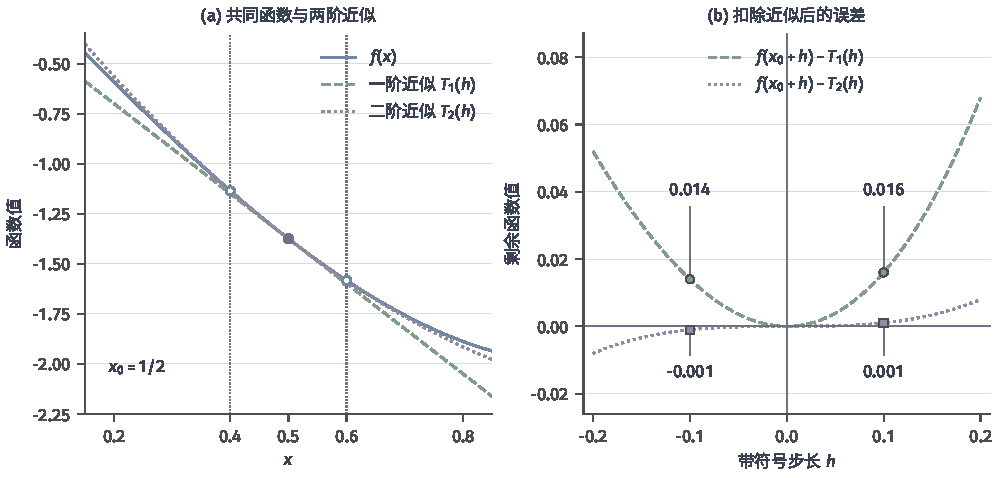
\includegraphics[width=169.0mm]{figures/00-shared/mathematical-preliminaries-upper/03-calculus/matplotlib/analysis-derivative-orders/figure.pdf}
 \caption{$f(x)=x^3-3x$在$x_0=1/2$处的Taylor近似，$h=x-x_0$。左图比较原函数、切线近似$T_1$与二次近似$T_2$；右图给出相应的带符号余项$3h^2/2+h^3$和$h^3$。标记点对应$h=\pm0.1$，余项的正负说明真值位于近似值的哪一侧。}
 \label{fig:analysis-derivative-orders}
\end{figure*}

\subsubsection{Peano余项}
如果只关心位移趋于零时误差的阶，可以不保留中间点，改用小量记号描述余项。
若$r\geq1$，$f$在包含$x_0$的某个开区间上属于$C^r$，则$h\to0$时
\[
 f(x_0+h)=\sum_{k=0}^r\frac{f^{(k)}(x_0)}{k!}h^k+o(|h|^r),
\]
称为带Peano余项的$r$阶Taylor公式。

推导时，对$r-1$阶Taylor公式使用Lagrange余项（这时定理~\ref{thm:analysis-taylor-lagrange}只要求$C^r$），得到$f(x_0+h)=T_{r-1}(x_0+h)+f^{(r)}(\xi_h)h^r/r!$，其中$\xi_h$位于$x_0$与$x_0+h$之间。把末项写成$f^{(r)}(x_0)h^r/r!$与$[f^{(r)}(\xi_h)-f^{(r)}(x_0)]h^r/r!$之和：前者与$T_{r-1}(x_0+h)$合成$T_r(x_0+h)$；后者除以$|h|^r$后趋于零，因为$\xi_h\to x_0$且$f^{(r)}$连续。这样就得到上式。

Peano余项描述局部误差的阶；若需要有限位移下的具体误差界，应使用Lagrange余项。$r=1$时上式就是式~\eqref{eq:analysis-scalar-first-order}，不过式~\eqref{eq:analysis-scalar-first-order}只需要$f$在该点可导。

\subsection{驻点的二阶导数判别}
在驻点处，Taylor公式的一阶项为零，函数在附近的增减就由二阶项决定。
设$a$是$f$的驻点，$f$在包含$a$的某个开区间上属于$C^2$。带Lagrange余项的一阶Taylor公式给出
\[
 f(a+h)-f(a)=\tfrac12f''(\xi_h)h^2,
\]
其中$\xi_h$位于$a$与$a+h$之间。若$f''(a)>0$，由$f''$的连续性，$h$充分小时$f''(\xi_h)\geq f''(a)/2>0$，所以每个充分小的非零$h$都使函数值严格增加，$a$为严格局部极小点。$f''(a)<0$时同理，$a$为严格局部极大点。

反之，在上述$C^2$条件下，局部极小点必须有$f''(a)\geq0$：若$f''(a)<0$，上一段说明$a$是严格局部极大点，附近其他点的函数值都严格小于$f(a)$，与局部极小矛盾。同理，局部极大点必须有$f''(a)\leq0$。

$f''(a)=0$时判别法没有结论：只知道前两阶导数，无法区分极小、极大与非极值。
\begin{example}[二阶导数为零时无法判别]
\label{ex:analysis-second-derivative-test-inconclusive}
考虑$x^4$、$-x^4$与$x^3$。三者在原点的一阶、二阶导数都为零：$(x^4)'=4x^3$、$(x^4)''=12x^2$，$(x^3)'=3x^2$、$(x^3)''=6x$，$-x^4$的导数只差一个符号。可是$x\neq0$时$x^4>0$，所以$0$是$x^4$的严格局部极小点；同理，$0$是$-x^4$的严格局部极大点；示例~\ref{ex:analysis-fermat-condition-failures}已说明$0$不是$x^3$的极值点。
\end{example}
回到示例~\ref{ex:analysis-cubic-stationary-points}，$f(x)=x^3-3x$有$f''(x)=6x$，$f''(1)=6>0$、$f''(-1)=-6<0$。二阶判别同样给出$1$为严格局部极小点、$-1$为严格局部极大点，与一阶导数判别的结论一致。

\FloatBarrier


\FloatBarrier
\section{本章小结}
\label{sec:analysis-summary}

连续性把输入的趋近与输出的趋近联系起来。一致连续、Lipschitz连续和绝对连续在此基础上分别加强控制：一致连续要求全定义域共用一个输入误差尺度，Lipschitz连续要求输出变化不超过输入距离的常数倍，绝对连续则控制许多短区间上的总变化。
这些条件的强弱必须连同定义域一起比较。在闭有界集上，连续与一致连续等价；实轴上的平方函数却只有逐点和局部的控制。
闭区间上的连续函数一定达到最小值和最大值，并取到两端值之间的每个值；后一结论还要求定义域是整个区间。

可微性把函数增量写成斜率乘输入增量再加高阶余项。四则运算、复合函数与反函数的求导规则，都由差商的极限或这种一阶展开得到。
Fermat定理、中值定理与单调性定理把一点处的导数与区间上的极值、增减和Lipschitz界联系起来；驻点是否为极值，可以由两侧导数的符号判别，也可以由二阶导数的符号判别。
Taylor公式用各阶导数构造局部多项式近似：Lagrange余项给出有限位移下的误差界，Peano余项描述位移趋零时的误差阶。

\chapter{一元函数的积分}
\label{chap:univariate-integration}
\label{chap:measurable-functions}

函数在区间上取不同的值时，怎样把这些值与所在范围的大小结合成一个累计量？反过来，累计得到的函数能否通过求导恢复原来的函数？
本章围绕这两个问题展开，用到第~\ref{chap:univariate-differentiation}章的连续性、导数与中值定理。

累计首先需要知道集合有多大。因此本章先从区间长度出发，经有限区间逼近与可数区间覆盖，建立实轴上的勒贝格测度，并说明零测集与几乎处处的含义。
有了集合的大小，再比较两种积分：黎曼积分沿区间分段取样，勒贝格积分按函数取值分层。两者在共同适用的范围内数值相同，勒贝格积分的适用范围更大，后面的累计统一采用它。
微积分基本定理分两个方向回答第二个问题：对累计函数求导能否得到被积函数，对导数积分能否得到原函数的增量。
最后讨论函数列与函数项级数的极限，说明连续性、导数与积分在什么条件下可以与极限交换，并用同一积分定义处理无穷区间与无界函数。

\section{集合的测量}
\label{sec:comb-set-measurement}
\label{sec:analysis-set-structures}

区间$[a,b]$的长度是$b-a$，但实轴上的集合未必是一个区间。
本节要解决的问题是：怎样把区间的长度推广到更一般的实数集合，并在原来的区间上仍得到$b-a$？
本章后面的积分需要这样的长度：把输入范围分成若干块后，只有知道各块的大小，才能按这些大小累计函数取值。
有限集合的元素个数与加权计数是另一类测量，可以先用它们说明为集合赋予大小时应遵守的相加规则。

集合的大小与点之间的距离是两种不同的结构。
在同一条实轴上使用同一种通常距离，既可以测量区间的长度，也可以数集合中的点；
因此，选定度量并不能唯一确定测度，即给集合赋予大小的方式。

本节先用有限集合的计数与加权计数说明相加规则，再从区间长度构造Jordan测量；有理点集将说明，只用有限个区间逼近还不够。
为此，随后利用可数集的列举规则改用可数覆盖，定义勒贝格外测度。
外测度对每个集合都有定义，却不保证不交部分精确相加，所以再用精确分割条件选出可测集，在可测集上得到可数可加的勒贝格测度。
最后推导勒贝格测度在集合列、零测集与几乎处处方面的性质，并用康托尔集说明零测集可以不可数。

\subsection{有限集与Jordan测量}
\label{sec:comb-counting-to-weight}

我们先把目标限制在有界的实数集合上，希望给这些集合建立与区间长度相容的测量方法。
例如$[0,1]\cup[2,3]$由两段互不重叠、长度各为$1$的区间组成，总长度应为$2$。
由这个例子可以看出所求测量应满足的一条规则：集合分成有限个两两不交的部分时，总量等于各部分测量值之和。

下面先在有限集合上用计数和加权计数说明这条规则，再回到实轴。
实轴上的长度将从区间出发：先计算有限个区间的并，再用这些简单集合从内、外两侧逼近更一般的有界集合；
只有当内部与外部的长度估计逼近同一个数时，才用这个数定义集合的Jordan测量。

\subsubsection{有限集的测量}

\paragraph{计数与加权计数}

在有限集合上，最直接的测量是数元素个数；若不同元素代表不同的份量，还可以给每个元素指定权重。
设$X=\{x_1,\ldots,x_m\}$中的点互异，每点带有非负权重$w_i$。
把落在$A\subseteq X$中的点的权重相加，定义
\[
 \mu(A)=\sum_{i:x_i\in A}w_i.
\]
所有$w_i=1$时，$\mu(A)=|A|$，即元素个数；改变权重时，元素不变，测量值却可以改变。
例如在$X=\{a,b\}$上给$a,b$分别指定权重$1,2$，就有$\mu(\{a\})=1$、$\mu(\{b\})=2$、$\mu(X)=3$。

若$A_1,\ldots,A_k$两两不交，并集中的每个点恰好落入其中一组，它的权重在等式两侧都只计一次，故
\[
 \mu\left(\bigcup_{j=1}^k A_j\right)=\sum_{j=1}^k\mu(A_j).
\]
这称为\term{有限可加性}（finite additivity）。它沿用计数的加法规则，
但相加的是各组的权重，不必是元素个数。

\paragraph{集合权重与函数值}

$\mu(A)$只测量集合$A$本身。后面还要在集合上累计函数取值，届时每个点的贡献等于函数值乘以该点的权重。
下面在同一个两点集合上比较等权与加权两种累计。
\begin{example}[两点集合上的等权与加权累计]
沿用$X=\{a,b\}$，给$a,b$分别指定权重$1,2$，并取函数值$f(a)=3$、$f(b)=-1$。

每点计$1$时，集合大小为$|X|=2$，函数的取值和为$f(a)+f(b)=3-1=2$。

按权重计时，集合大小为$\mu(X)=1+2=3$，函数的加权和为
\[
 3\cdot1+(-1)\cdot2=1.
\]
\end{example}

同一组元素和同一组函数值，在两种权重下给出不同的集合大小（$2$与$3$），也给出不同的累计值（$2$与$1$）。
表~\ref{tab:analysis-metric-measure-integral}汇总这些计算；本章后面的积分将把这种加权累计推广到更一般的集合与函数。
\begin{table}[htbp]
 \centering\small
 \begin{tabularx}{\linewidth}{@{}lXX@{}}
 \toprule
 考察对象 & 所用规则 & $X=\{a,b\}$上的结果\\
 \midrule
 元素个数 & 每点计$1$ & $|X|=2$\\
 集合权重 & $a,b$分别计$1,2$ & $\mu(X)=3$\\
 数值的等权累计 & 取值为$3,-1$ & $3-1=2$\\
 数值的加权累计 & 同一取值采用权重$1,2$ & $3-2=1$\\
 \bottomrule
 \end{tabularx}
 \caption{有限计数与加权累计。相同的元素范围和相同的数值取值仍可采用不同权重；只有先固定权重，累计值才有确定含义。}
 \label{tab:analysis-metric-measure-integral}
\end{table}

\paragraph{点数与长度}

有限集合的例子说明了不交部分如何相加，但每点计$1$的规则不能给出区间长度。
例如$[0,1]$和$[0,2]$都含有无限多个点，逐点计数都得到无穷，而它们的长度分别应为$1$和$2$。
所以，要推广区间长度，必须另行规定与几何长度相容的测量规则。

单点$[a,a]$的长度为$0$，有限个单点的并也应有长度$0$。
这与非退化区间的长度为正并不矛盾：非退化区间含无限多个点，不能写成有限个单点的并，所以有限可加性不适用于把它拆成全部单点的操作。
第~\ref{sec:analysis-countable-outer-measure}节讨论可数覆盖时还要用到另一事实：非退化区间的点也不能列成一个序列。

因此我们改以区间长度为起点：先计算能由有限个区间组成的集合的长度，再研究不能这样表示的集合。

\subsubsection{Jordan测量}

\paragraph{区间长度与初等集}

一个区间的长度由端点决定；有限个区间组成的集合，也可以先拆成互不重叠的小段再相加。
对端点为$a\leq b$的有界区间$I$，规定长度为$\ell(I)=b-a$，不因端点是否包含而改变；
单点与空集的长度为$0$。

为反复使用这类可以直接计算长度的集合，先给它们一个名称：
我们把有限个这样的区间的并称为\term{初等集}（elementary set），空集也约定为初等集。
例如$[0,1]\cup[2,3]$是初等集，两段长度相加得到$2$。
区间发生重叠时，需要先消除重复计算：$[0,2]\cup[1,3]=[0,3]$的长度为$3$，不能把原来两段的长度直接相加为$4$。

一个初等集$B$可以有多种区间表示，所以先按一种表示规定长度，再检查结果与表示无关。
取定一种表示，将其中所有端点排序，按相邻端点之间的开区间及端点本身切分，得到有限个两两不交的小段；把属于$B$的小段长度相加，记为$\ell(B)$。
若采用另一种表示，把两组端点合在一起排序，便得到两种切分的共同细分。
区间从$c$处分成两段时，$(c-a)+(b-c)=b-a$，所以细分不改变总长度。
因此，两种表示给出同一个$\ell(B)$。

对有限个初等集取它们端点的共同细分可知，初等集的并、交、差仍为初等集，不交初等集的长度有限可加。
一般的有限覆盖只给出不等式：若$B\subseteq\bigcup_{j=1}^k B_j$，则
$\ell(B)\leq\sum_{j=1}^k\ell(B_j)$，因为在共同细分下，$B$的每个小段在右侧至少计算一次，重叠的小段还会被重复计算。
特别地，取$k=1$可知$A\subseteq B$时$\ell(A)\leq\ell(B)$。

\paragraph{内容量与外容量}

初等集的长度已经可以计算，但有界集合只要求一个集合包含在某个有限区间内，并不要求它本身由有限个区间组成。
下面的倒数点集就是这样的集合。
\begin{example}[倒数点集不是初等集]
\label{ex:set-measure-reciprocal-not-elementary}
考虑
\[
 E=\{1,1/2,1/3,\ldots\}\subseteq[0,1].
\]
它包含于$[0,1]$，因此有界。

对任意$u>0$，$E\cap[u,1]$中的点$1/n$都满足$n\leq1/u$，所以这一部分只有有限多个点。

由此可知$E$不包含任何正长度区间。假如$E$包含端点为$c<d$的区间，由$E\subseteq(0,1]$可知$c\geq0$；
取$u=(c+d)/2>0$，区间中的$[u,d)$便落在$E\cap[u,1]$中。它含无限多个点，与上一步的有限性矛盾。

若$E$是初等集，组成它的每个区间都包含于$E$，只能是单点或空集，于是$E$只有有限多个点；这与$E$含无限多个点矛盾。
所以$E$不是初等集。
\end{example}

因此初等集的长度公式不能直接用于$E$。
为了测量$E$这样的集合，一种办法是保留初等集作为计算工具，用包含关系给出长度估计。
把初等集$A$放在$E$内部，即$A\subseteq E$，$\ell(A)$就应是$E$的长度的下界；
用初等集$B$包住$E$，即$E\subseteq B$，$\ell(B)$就应是上界。
我们希望内部估计尽可能大、外部估计尽可能小，因此分别取内部长度的上确界与外部长度的下确界。
这两个数未必相等；若相等，内部与外部的估计就共同确定了一个长度值，可以把它作为$E$的测量值。

下面给这两个界命名，并按它们是否相等规定哪些有界集合可以用这种方法测量；两侧的候选都是初等集，长度都按初等集的长度$\ell$计算。
\begin{definition}[Jordan内容量与外容量]
\label{def:analysis-jordan-content}
对有界集合$E\subseteq\mathbb R$，定义\term{Jordan内容量}（Jordan inner content）与\term{Jordan外容量}（Jordan outer content）为
\[
 \begin{aligned}
 j_*(E)&=\sup\{\ell(A):A\subseteq E,\ A\text{为初等集}\},\\
 j^*(E)&=\inf\{\ell(B):E\subseteq B,\ B\text{为初等集}\}.
 \end{aligned}
\]
若$j_*(E)=j^*(E)$，称$E$为Jordan可测集，二者的共同值记为$j(E)$，称为它的\term{Jordan测量}（Jordan measure）值。
\end{definition}

对有界集合$E$，有界性保证外部候选非空且长度有限，空集则是内部候选；
又由$A\subseteq E\subseteq B$和初等集长度的单调性得$\ell(A)\leq\ell(B)$。所以
$0\leq j_*(E)\leq j^*(E)<\infty$。
上下确界一般不要求由某个最佳初等集取得；若$E$本身是初等集，内外都可以取$E$，结合$\ell(A)\leq\ell(E)\leq\ell(B)$便得$j_*(E)=j^*(E)=\ell(E)$。
所以新的定义保留了区间长度与有限区间并的长度，有限点集的测量值也仍为$0$。

倒数点集虽然不是初等集，它的两个容量却可以直接算出。
\begin{example}[倒数点集的Jordan测量为零]
\label{ex:set-measure-reciprocal-jordan-null}
仍取$E=\{1/n:n\geq1\}$。

内部：示例~\ref{ex:set-measure-reciprocal-not-elementary}已说明$E$不含正长度区间，所以包含于$E$的初等集只能由有限个单点组成，长度为$0$。于是
\[
 j_*(E)=0.
\]

外部：对每个整数$N\geq2$，取
\[
 B_N=\{1,1/2,\ldots,1/(N-1)\}\cup[0,1/N].
\]
前$N-1$个点分别由单点覆盖，其余的点$1/n$（$n\geq N$）全部落在$[0,1/N]$内，故$E\subseteq B_N$。
$B_N$是初等集，有限个单点不增加长度，所以$\ell(B_N)=1/N$。
于是$0\leq j^*(E)\leq1/N$对所有$N\geq2$成立，从而
\[
 j^*(E)=0.
\]

内外容量相等，所以$E$是Jordan可测集，且$j(E)=0$。
\end{example}

这个不属于初等集的无限点集仍然Jordan可测。
它的测量值来自有限逼近：外部候选的长度$1/N$可以任意小，内部候选的长度始终为$0$。

\paragraph{有限逼近与可加性}

内外数值相等也可以改写成误差条件：$E$为Jordan可测集，当且仅当对每个$\varepsilon>0$，
存在初等集$A\subseteq E\subseteq B$，使$\ell(B)-\ell(A)<\varepsilon$。
若$E$可测，按上确界和下确界的定义，各选一个与共同值$j(E)$相差小于$\varepsilon/2$的内部候选和外部候选即可。
反过来，若对每个$\varepsilon$都有这样的$A,B$，则$\ell(A)\leq j_*(E)\leq j^*(E)\leq\ell(B)$，两个容量之差小于任意正数，只能相等。

这个误差条件还保证有限次集合运算保持Jordan可测性。
分别以$A_E\subseteq E\subseteq B_E$和$A_F\subseteq F\subseteq B_F$夹住两个Jordan可测集，
它们的并夹在$A_E\cup A_F$与$B_E\cup B_F$之间，且
\[
 (B_E\cup B_F)\setminus(A_E\cup A_F)\subseteq(B_E\setminus A_E)\cup(B_F\setminus A_F).
\]
初等集$A\subseteq B$时，有限可加性给出$\ell(B)-\ell(A)=\ell(B\setminus A)$；再用有限覆盖不等式，新上下界的长度差不超过原来两份误差之和。

交集夹在$A_E\cap A_F$与$B_E\cap B_F$之间，差集$E\setminus F$夹在$A_E\setminus B_F$与$B_E\setminus A_F$之间。
两种情形中，外部逼近与内部逼近之差同样包含于$(B_E\setminus A_E)\cup(B_F\setminus A_F)$。
因此，Jordan可测集的有限并、交、差仍Jordan可测。

若$E,F$还不交，内部逼近$A_E,A_F$也不交。左端用不交初等集的有限可加性，右端用有限覆盖不等式，得到
\[
 \ell(A_E)+\ell(A_F)
 \leq j_*(E\cup F)\leq j^*(E\cup F)
 \leq\ell(B_E)+\ell(B_F).
\]
让各份逼近误差趋于零，两端都趋于$j(E)+j(F)$，所以$j(E\cup F)=j(E)+j(F)$。
这就是Jordan测量的有限可加性。论证中只合并了有限份逼近误差，所以它不能直接推广到无限多个集合的并。

\subsubsection{Jordan测量的局限}

\paragraph{有理点集的内外容量}

倒数点集$E$虽然不是初等集，仍能用有限区间并把外部长度压到任意小。
这是否意味着每个有界集合都能这样处理？下面考察$Q_0=\mathbb Q\cap[0,1]$，它将说明Jordan方法使用的有限逼近不能处理任意的有界集合。

先看$Q_0$在区间中的分布：任意非退化实区间$(a,b)$（$a<b$）都含有理数和无理数。
找有理数时，取正整数$q>1/(b-a)$，使相邻分数$p/q$与$(p+1)/q$的间距$1/q$小于区间长度。
令$p$为满足$p>aq$的最小整数，则$(p-1)/q\leq a<p/q$，于是$p/q\leq a+1/q<b$，即$p/q\in(a,b)$。

找无理数时，对区间内的有理数$r$，取正整数$k$使$\sqrt2/k<b-r$，则$r+\sqrt2/k$位于$(r,b)$内；
它若是有理数，$\sqrt2=k\bigl((r+\sqrt2/k)-r\bigr)$也将是有理数，矛盾。
所以$Q_0$和它在$[0,1]$内的补集都与$[0,1]$的每个正长度子区间相交。

利用这种分布，可以算出$Q_0$的两个容量。
\begin{example}[有理点集不Jordan可测]
\label{ex:set-measure-rationals-not-jordan}
设$Q_0=\mathbb Q\cap[0,1]$。

内部：任何正长度区间都含无理数，不可能完全落在$Q_0$中。
包含于$Q_0$的初等集因此只能由有限个单点组成，长度为$0$，所以
\[
 j_*(Q_0)=0.
\]

外部：设初等集$B$包含$Q_0$。把组成$B$的有限个区间的端点补齐，得到闭包$\overline B$；
补上有限个点不改变长度，所以$\ell(\overline B)=\ell(B)$。
若$[0,1]$内某点$x$不在$\overline B$中，由于$\overline B$是闭集，$x$附近就有一小段开区间完全避开$\overline B$，从而也避开$B$。
这段开区间在$[0,1]$内的部分仍有正长度，因而含有有理数，与$Q_0\subseteq B$矛盾。
因此$[0,1]\subseteq\overline B$，从而$\ell(B)=\ell(\overline B)\geq1$。
又因为$[0,1]$本身就是一个外部候选，得到
\[
 j^*(Q_0)=1.
\]

两个容量相差$1$，所以$Q_0$不Jordan可测。
\end{example}

\paragraph{有限覆盖的限制}

$Q_0$不Jordan可测（示例~\ref{ex:set-measure-rationals-not-jordan}），原因不在于有限覆盖中的区间还不够多。
无论选一百个还是一百万个区间，只要仍是有限个，它们的并就是初等集，例中的论证仍迫使任何覆盖$Q_0$的总长度至少为$1$。
倒数点集的情形不同：它可以把除有限个点以外的全部点装进靠近零的一个短区间；
有理点集却在$[0,1]$的每一小段中都出现，不能用一个越来越短的区间收拢剩下的点。

要突破这个下界，需要扩大允许使用的覆盖，而不是继续增加一次有限覆盖中的区间数。
如果能将$Q_0$列为$q_1,q_2,\ldots$，就可以给每个点分别安排一个开区间，
并把长度依次限制为$\varepsilon/2,\varepsilon/4,\varepsilon/8,\ldots$。
这样每个点都会被覆盖，总长度又由几何级数控制在$\varepsilon$以内，而$\varepsilon$可以任意小。
这里需要一整列区间共同覆盖全部点，其中任意有限前段本身都未必覆盖$Q_0$。

图~\ref{fig:measure-countable-cover}对比了两种覆盖规则；右侧的前四项只展示长度如何分配，并未单独完成对全部有理点的覆盖。

\begin{figure*}[htbp]
 \centering
 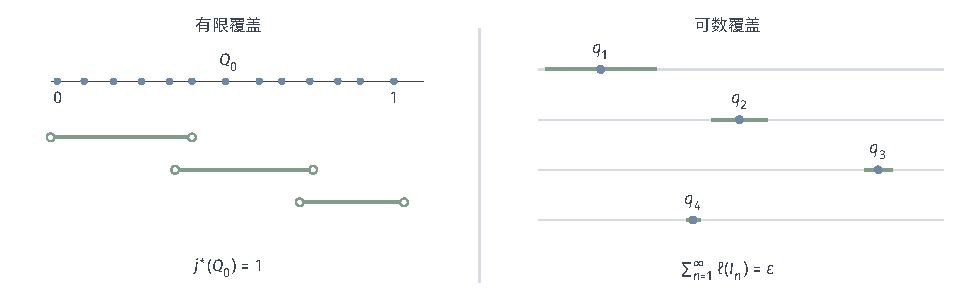
\includegraphics[width=169mm]{figures/00-shared/mathematical-preliminaries-upper/03-calculus/tikz/measure-countable-cover/figure.pdf}
 \caption{有限覆盖与可数覆盖。左侧画出一个有限开区间覆盖示例；对$Q_0=\mathbb Q\cap[0,1]$的任意有限区间覆盖，总长度均不小于$1$。右侧将一次完整覆盖改为可数个区间，图中取$\varepsilon=0.8$，只画列举中前四个点及其区间，长度依次为$\varepsilon2^{-n}$；使用全部区间时覆盖全部有理点，总长度为$\varepsilon$，并可随$\varepsilon$任意减小。点的有限示意不能表示有理点的完整稠密分布。}
 \label{fig:measure-countable-cover}
\end{figure*}

由此得到新的做法：允许用可数个区间组成一次完整覆盖，再用非负级数计算总长度。
实施这一做法需要第~\ref{sec:comb-countable-sets}节建立的列举与合并规则；下一小节从这些规则出发，定义新的外部长度估计。

\subsection{可数集与勒贝格外测度}
\label{sec:analysis-countable-outer-measure}

有限覆盖的限制已经说明了改变构造的理由：既要让每个可列举的点都分到自己的小区间，又要把所有区间的总长度控制住。
可数覆盖能同时做到这两件事，因为区间带有自然数编号，长度可以用已经学过的非负级数相加。

这一做法要用于后面的推导，还需要两项工具：可数个可数集合的并仍可数，保证合并若干组覆盖后仍是允许的覆盖；
非负双重级数可以合并，保证按组计算与统一编号计算得到同一个总长度。
这些工具建立后，就能定义勒贝格外测度，并检查它既能改进有理点集的估计，又保留普通区间的长度。

\subsubsection{可数覆盖的编号与长度}

第~\ref{sec:comb-countable-sets}节已定义可数集，并用对角列举证明自然数对、有理数与可数个可数集的并都可数。
因此$Q_0=\mathbb Q\cap[0,1]$可以列为$q_1,q_2,\ldots$，每个点都能分到自己的小区间；
合并一列可数覆盖时，所有区间也仍可统一编号。
余下要检查的是总长度：改变非负项的列举方式，不能改变覆盖长度的总和。

\paragraph{非负双重级数的合并}

沿用第~\ref{sec:analysis-continuous-limits}节对非负项级数规定的扩展总和，对$a_n\in[0,\infty]$有
\begin{equation}
 \sum_{n=1}^{\infty}a_n
 =\sup_{N\geq1}\sum_{n=1}^Na_n\in[0,\infty].
 \label{eq:comb-nonnegative-sum-supremum}
\end{equation}
非负性使有限和随加入新项而不减，所以也可以对所有有限索引集取上确界，结果相同。

对$a_{n,j}\geq0$，将双指标按任一无遗漏、无重复的顺序列成一个序列；由上一句，它的总和总是
\[
 S=\sup_{F\subseteq\mathbb N_+^2,\,F\text{有限}}
          \sum_{(n,j)\in F}a_{n,j},
\]
与所选顺序无关。下面证明$S=\sum_n\sum_j a_{n,j}$，即$S$等于先对每一行求和、再把各行之和相加的结果。

一方面，任取有限索引集$F$，它只涉及有限多行，并在每一行中只取有限多项；
每行取出的部分不超过该行之和，所以$\sum_{(n,j)\in F}a_{n,j}\leq\sum_n\sum_ja_{n,j}$。对$F$取上确界，得$S\leq\sum_n\sum_ja_{n,j}$。

另一方面，固定行数$N$与任意$\varepsilon>0$。若前$N$行之和都有限，对每个$n\leq N$选有限列数$J_n$，
使该行前$J_n$项之和超过整行之和减去$\varepsilon/N$。这些项组成一个有限索引集，所以
$S\geq\sum_{n=1}^N\sum_ja_{n,j}-\varepsilon$。令$\varepsilon\downarrow0$，再对$N$取上确界，得到$S\geq\sum_n\sum_ja_{n,j}$。
若某行之和为无穷，它的有限部分和可以超过任意给定的有限上界，同样迫使$S=+\infty$，此时两侧都为无穷。

这个证明只用到有限和与上确界的性质，因此这里的非负项换序不必借助后文的积分换序定理。

\subsubsection{勒贝格外测度}
\label{sec:comb-length-and-lebesgue-measure}

\paragraph{可数区间覆盖}

由于$Q_0$可以列为$q_1,q_2,\ldots$，逐点安排小区间的方案可以实施。
我们把这种覆盖方式用于一般集合：对$E\subseteq\mathbb R$，若有限或可数个有界开区间$I_j=(a_j,b_j)$满足$E\subseteq\bigcup_j I_j$，就称它们为$E$的可数区间覆盖。
区间可以重叠，也可以伸出$E$；它们的总长度为非负级数$\sum_j(b_j-a_j)$，允许等于$+\infty$。

“可数”限制的是覆盖区间的个数，不是$E$中的点数；一个开区间就可以覆盖含有不可数多个点的闭区间。
选择可数覆盖，是为了能逐项分配误差、用级数累计长度，并在合并覆盖时保留这两种能力。
前面没有给任意不可数族定义总长度，因此这里也不把“可数”放宽为不受限制的任意区间族。
采用开区间，则是为了在证明中使用闭区间的有限子覆盖性质；下面将用它保证原来的区间长度不被改变。

\paragraph{勒贝格外测度的定义}

一次覆盖可能伸出集合，也可能重复覆盖某些位置，所以它的总长度只是一个依赖于区间选择的外部估计。
为了尽量排除这些额外长度，我们对所有允许覆盖的总长度取下确界，得到勒贝格外测度。
\begin{definition}[勒贝格外测度]
\label{def:analysis-lebesgue-outer-measure}
对$E\subseteq\mathbb R$，定义其\term{勒贝格外测度}（Lebesgue outer measure）为
\begin{equation}
 m^*(E)=\inf\left\{\sum_{j=1}^{\infty}(b_j-a_j):
 \begin{array}{l}
 E\subseteq\bigcup_{j=1}^{\infty}(a_j,b_j),\\
 -\infty<a_j<b_j<\infty
 \end{array}\right\}.
 \label{eq:comb-lebesgue-outer-measure}
\end{equation}
这里也允许有限覆盖以及空集的空覆盖；空和为$0$。
\end{definition}

任意集合都能由覆盖整条实轴的一列区间覆盖，所以候选始终非空。
下确界可以为无穷，也不必由某个覆盖达到。
例如单点可以被任意短的开区间覆盖，其外测度为$0$；但任何覆盖都至少含一个非空开区间，总长度为正，所以没有覆盖能达到这个下确界。

\paragraph{空集与单调性}

空覆盖表明$m^*(\varnothing)=0$。
若$E\subseteq F$，任何覆盖$F$的区间族也覆盖$E$，
所以$F$的每个候选也是$E$的候选；在更大的候选集合上取下确界，结果不会更大，便得$m^*(E)\leq m^*(F)$。
这称为外测度的单调性，依据是两组候选覆盖之间的包含关系。

\paragraph{区间的外测度}

允许可数覆盖后，候选更多，下确界可能下降。我们希望有理点集的估计下降，但也必须检查普通区间的长度没有因此改变。
\begin{lemma}[区间的外测度等于长度]
\label{lem:set-measure-interval-outer-measure}
设$a<b$。对端点为$a,b$的有界区间$I$（两端可含可不含），有$m^*(I)=b-a$；无界区间的外测度为$+\infty$。
\end{lemma}
\begin{proof}
先证明$m^*([a,b])=b-a$。

上界：对任意$\varepsilon>0$，单个开区间$(a-\varepsilon/2,b+\varepsilon/2)$覆盖$[a,b]$，长度为$b-a+\varepsilon$。
令$\varepsilon\downarrow0$，得$m^*([a,b])\leq b-a$。

下界：这一侧必须控制每一种可数覆盖，不能只考察某一组区间。
任取$[a,b]$的可数开区间覆盖$\{(a_j,b_j)\}$。由闭区间的有限子覆盖性质（定理~\ref{thm:analysis-interval-finite-subcover}），其中有限个区间已经覆盖$[a,b]$；记它们的索引集为$F$。
初等集的有限覆盖不等式给出
\[
 b-a\leq\sum_{j\in F}(b_j-a_j)\leq\sum_{j=1}^{\infty}(b_j-a_j).
\]
对所有可数覆盖取下确界，得$m^*([a,b])\geq b-a$。

其他有界区间$I$包含长度任意接近$b-a$的闭区间，又有$I\subseteq[a,b]$，由单调性夹逼得$m^*(I)=b-a$。
无界区间包含任意长的有界闭区间，所以外测度为$+\infty$。
\end{proof}

所以改用可数覆盖后，区间的长度保持原值。

\paragraph{可数点集的外测度}

现在回到推动构造的例子，检验可数覆盖是否真正突破了有限覆盖的限制。
\begin{example}[可数点集的外测度为零]
\label{ex:set-measure-countable-outer-null}
设$E=\{x_1,x_2,\ldots\}$可数。任给$\varepsilon>0$，对每个$n$取
\[
 I_n=\bigl(x_n-\varepsilon2^{-n-1},\ x_n+\varepsilon2^{-n-1}\bigr).
\]
每个点$x_n$都落入$I_n$，所以这列区间覆盖全部$E$，且$\ell(I_n)=\varepsilon2^{-n}$。
于是
\[
 0\leq m^*(E)\leq\sum_{n=1}^{\infty}\varepsilon2^{-n}=\varepsilon.
\]
由于$\varepsilon$任意，$m^*(E)=0$。有限集只需用前有限个区间，同样得到外测度为$0$。
\end{example}

例中每个覆盖区间的长度都为正；趋于零的是整组覆盖的总长度上界，而不是一些未定义的正“无穷小”之和。

特别地，$m^*(Q_0)=0$，尽管$Q_0$的Jordan外容量为$1$。
有限覆盖的总长度不能低于$1$，可数覆盖却能把总长度压到任意给定的正数以内；改变的是一次完整覆盖所允许使用的区间族。
这与$m^*([0,1])=1$也不矛盾：$Q_0$可数，能够逐点编号；整个区间却不可数，无法给其中全部点各分配一个自然数编号，例中的覆盖方式不能用于$[0,1]$。

$m^*(Q_0)=0$回答的是外部估计能否下降的问题。
到这里，每个集合都已有外测度值，但还没有证明不交集合的外测度能够精确相加；要把外测度用于分块累计，还需要下面的可加性与可测性。

\subsubsection{可数可加性}

\paragraph{可数可加性的要求}

新的覆盖方式已经能累计可数个区间的长度，我们也希望测量规则能处理可数次不交分割。
例如，若一个可数点集作为各个单点的不交并参与精确相加，它的总长度就应等于单点长度之和。

一般地，对一个给集合赋值的映射$\nu$，希望有
\[
 \nu\left(\bigcup_{n=1}^{\infty}E_n\right)=\sum_{n=1}^{\infty}\nu(E_n),
 \qquad E_i\cap E_j=\varnothing\ (i\neq j),
\]
其中并集与各部分都应在$\nu$的赋值范围内。
这称为\term{可数可加性}（countable additivity），右侧是已经定义的非负项级数。

区间不可数，所以这一要求不允许把区间拆成全部单点后当作可数级数求和；
单点外测度为零与区间外测度为正并不矛盾。

\paragraph{外测度的可数次可加性}

已经建立的覆盖构造能先保证一个较弱的结论：把每个集合的覆盖合并，就得到并集的覆盖，
所以并集的外测度不超过各部分外测度之和。这只是不等式，并且不要求各集合不交。
这项性质称为\term{可数次可加性}（countable subadditivity）；名称中的“次”表示这里保证的是上界，不是精确相等。

每个集合未必有达到外测度的最优覆盖，证明时只能选近似最优覆盖。
因此需要把第$n$组的误差限制为$\varepsilon2^{-n}$，使合并无穷多组后总误差仍不超过$\varepsilon$。
\begin{theorem}[勒贝格外测度的可数次可加性]
\label{thm:analysis-outer-subadditivity}
对任意$E_1,E_2,\ldots\subseteq\mathbb R$，有
\begin{equation}
 m^*\left(\bigcup_{n=1}^{\infty}E_n\right)
 \leq\sum_{n=1}^{\infty}m^*(E_n).
 \label{eq:analysis-outer-subadditivity}
\end{equation}
\end{theorem}
\begin{proof}
若右侧为$+\infty$，不等式直接成立。
设右侧有限，则每个$m^*(E_n)$有限。给定$\varepsilon>0$，由下确界定义，
为每个$E_n$选择覆盖$\{I_{n,j}:j\geq1\}$，使
\[
 E_n\subseteq\bigcup_j I_{n,j},\qquad
 \sum_j\ell(I_{n,j})<m^*(E_n)+\varepsilon2^{-n}.
\]
空集可以取空覆盖，有限覆盖直接作为有限组处理。
所有$I_{n,j}$覆盖$\bigcup_nE_n$；可数个可数集的并仍可数，故它们是允许使用的一组覆盖。
再由非负双重级数的合并规则，
\[
 \begin{aligned}
 m^*\left(\bigcup_nE_n\right)
 &\leq\sum_{n,j}\ell(I_{n,j})\\
 &=\sum_n\sum_j\ell(I_{n,j})
 \leq\sum_nm^*(E_n)+\varepsilon.
 \end{aligned}
\]
最后让$\varepsilon\downarrow0$，得到所需不等式。
\end{proof}

\paragraph{一般外测度}

刚才的证明只给出不等式，尚未要求不交集合的值精确相加。
空集取值为零、单调性与可数次可加性这三条性质不依赖区间长度的具体形式；把它们抽取出来，便得到可用于其他测量构造的一般概念。
\begin{definition}[外测度]
\label{def:analysis-outer-measure}
集合$X$上的映射$\mu^*:\mathcal P(X)\to[0,\infty]$，若满足
\[
 \begin{gathered}
 \mu^*(\varnothing)=0,\\
 A\subseteq B\Longrightarrow\mu^*(A)\leq\mu^*(B),\\
 \mu^*\left(\bigcup_{n=1}^{\infty}E_n\right)\leq\sum_{n=1}^{\infty}\mu^*(E_n)
 \quad(E_n\subseteq X),
 \end{gathered}
\]
则称为\term{外测度}（outer measure）。
\end{definition}
前面已经证明勒贝格外测度满足这三条，所以它是外测度的一个实例；其中第三条来自覆盖的合并，而覆盖合并没有给出反向不等式。
即使$E_n$两两不交，分别覆盖它们的开区间也可能彼此重叠；集合不交并不会使覆盖的长度自动精确相加。
反过来，把覆盖并集的区间按任意集合切开，所得部分又未必是区间，不能直接沿用区间长度公式来分配总量。
因此，不能仅凭这三个条件便把式~\eqref{eq:analysis-outer-subadditivity}中的不等号改为等号。

下一步要补上的，是集合与这套外部估计之间的分割相容性：用一个集合切分任意测试集，切分后两部分的外测度之和仍等于原值。
我们将把满足这个要求的集合选出来，再证明在它们组成的范围内，不交可数并确实能够精确相加。

\subsection{可测集与勒贝格测度}
\label{sec:analysis-lebesgue-measurable-construction}

现在需要区分两个问题：一个集合能否取得外测度值，以及它能否在分割计算中保持精确相加。
第一个问题已经解决，任意集合都有$m^*$值；第二个问题还没有由覆盖构造保证。
要为积分准备可以反复分块的测量规则，就需要找出能够保持精确分割的集合，这就是引入可测集的原因。

下面保留原来的$m^*$数值，要求一个集合用来切分任何测试集时，都不改变分割前后的总量。
我们先写出这个条件，再证明满足条件的集合对取补和可数并封闭，最后证明限制到这一范围的$m^*$具有可数可加性。

\subsubsection{可测性的要求}

\paragraph{精确分割}

固定一个待检验的集合$A$，再任取测试集$E$。$A$把$E$分成落在$A$内的部分和落在$A$外的部分：
\[
 E=(E\cap A)\cup(E\setminus A),\qquad
 (E\cap A)\cap(E\setminus A)=\varnothing.
\]
次可加性已经保证$m^*(E)\leq m^*(E\cap A)+m^*(E\setminus A)$。
若要分割不改变总量，还需要反向不等式；缺少它时，两部分分别作外部估计，所得总和可能比整体的外部估计大。

外测度的三条公理确实不能自动排除这种情况，下面的两点空间就是一个有限例子。
\begin{example}[两点空间上不可加的外测度]
\label{ex:set-measure-two-point-outer-measure}
在两点集合$X=\{a,b\}$上，令$\mu^*(\varnothing)=0$，并令每个非空子集的值都为$1$。

单调性：若$A\subseteq B$且$A$非空，则$B$也非空，两者的值都为$1$；若$A$为空集，则$\mu^*(A)=0\leq\mu^*(B)$。

可数次可加性：若一列子集的并为空，各项都是空集，两侧均为$0$；若并非空，至少有一项非空，右侧至少为$1$，不小于左侧的$1$。

所以$\mu^*$是外测度。但取$E=X$、$A=\{a\}$时，
\[
 1=\mu^*(X)<\mu^*(\{a\})+\mu^*(\{b\})=2,
\]
即集合$\{a\}$不能精确分割测试集$X$。
\end{example}

这个例子只说明仅有三条公理不足以推出精确相加，并不是勒贝格外测度下的不可测集构造。
图~\ref{fig:measure-exact-splitting}把它与区间的精确分割放在一起，展示可测性条件要排除的总量变化。

\begin{figure*}[htbp]
 \centering
 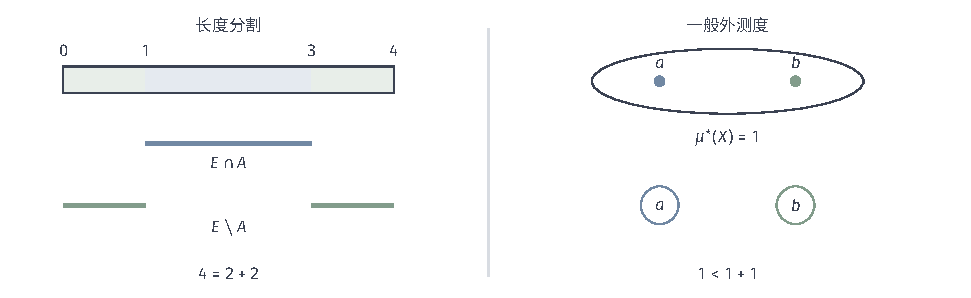
\includegraphics[width=169mm]{figures/00-shared/mathematical-preliminaries-upper/03-calculus/tikz/measure-exact-splitting/figure.pdf}
 \caption{精确分割与一般外测度的差别。左侧用$A=[1,3]$分割测试集$E=[0,4]$，落在$A$内的长度为$2$，外部两段总长度也为$2$，两者恢复原来的$4$；有限端点不改变长度。右侧使用正文两点空间的外测度，整体值为$1$，拆成两个单点后的值之和为$2$。右侧并非勒贝格不可测集的图像；左侧也只画了一个测试集，可测性定义要求对每个测试集都有精确等式。}
 \label{fig:measure-exact-splitting}
\end{figure*}

勒贝格外测度也存在不能保持精确分割的集合；这类不可测集的存在与构造可参考测度论教材\scite{math-hunter2011measure,math-folland1999real}，这里不展开。
下面直接以精确分割为条件选取可测集，并证明这类集合上的可加性。

\paragraph{可测集的定义}

我们希望$A$能够在不同范围的计算中反复参与分割，因此条件不能只针对某个预先选好的$E$，而要对所有测试集成立。
满足这一要求的$A$称为勒贝格可测集。
\begin{definition}[勒贝格可测集]
\label{def:analysis-lebesgue-measurable-set}
集合$A\subseteq\mathbb R$称为\term{勒贝格可测集}（Lebesgue measurable set），若对每个$E\subseteq\mathbb R$都有
\begin{equation}
 m^*(E)=m^*(E\cap A)+m^*(E\setminus A).
 \label{eq:comb-caratheodory-measurability}
\end{equation}
全体勒贝格可测集组成的集合族记为$\mathcal L(\mathbb R)$。
\end{definition}

式~\eqref{eq:comb-caratheodory-measurability}称为Carathéodory可测性条件。
由于$m^*(E)\leq m^*(E\cap A)+m^*(E\setminus A)$已由次可加性保证，验证可测性只需证明
$m^*(E)\geq m^*(E\cap A)+m^*(E\setminus A)$。
条件必须对每个$E$检验：只令$E=A$得到的是$m^*(A)=m^*(A)+m^*(\varnothing)$，对任意集合都成立，无法区分哪些分割与外测度相容。
“可测”并不表示此前无法给$A$求值；$m^*(A)$对任意$A$都已定义，新增的要求是$A$与所有测试集的分割相容。

外测度为零的集合不需要逐个验证分割；下面的引理一次处理所有这样的集合及其子集，以后处理零测余量和完备性时都会用到。
\begin{lemma}[零外测度集的子集可测]
\label{lem:analysis-zero-outer-measure-measurable}
若$N\subseteq\mathbb R$且$m^*(N)=0$，则每个$D\subseteq N$都勒贝格可测，并且$m^*(D)=0$。
\end{lemma}
\begin{proof}
单调性先给出$m^*(D)=0$。对任意测试集$E$，有
\[
 m^*(E\cap D)+m^*(E\setminus D)=0+m^*(E\setminus D)\leq m^*(E).
\]
结合外测度次可加性给出的反向不等式，得到可测性所需的精确分割等式。
\end{proof}

由示例~\ref{ex:set-measure-countable-outer-null}，$m^*(Q_0)=0$，所以此引理立即说明$Q_0$勒贝格可测。
利用$Q_0$的可测性，还可以算出$[0,1]$中无理点集的外测度。
\begin{example}[单位区间中无理点的外测度]
\label{ex:set-measure-irrationals-outer-measure}
在$Q_0$的可测性条件中取测试集$E=[0,1]$。由于$E\cap Q_0=Q_0$、$E\setminus Q_0=[0,1]\setminus Q_0$，得到
\[
 1=m^*([0,1])=m^*(Q_0)+m^*([0,1]\setminus Q_0)=0+m^*([0,1]\setminus Q_0).
\]
所以$[0,1]$中无理点组成的集合外测度为$1$。
\end{example}

有理点与无理点都分布在$[0,1]$的每一小段中，却不因此占有相同的长度。
可测性由分割等式判断，而不是由集合看起来是否稠密、光滑或规则判断。

\subsubsection{可测集族}

前面的定义逐个检验一个集合能否精确切分任意测试集。接下来还要检验：可测集经过取补、合并等运算后，是否仍然可测？

如果每次分块或合并都可能离开允许测量的范围，就无法反复使用这套测量方法。
Jordan测量就有这个问题：每个单点$\{q_n\}$都Jordan可测，它们的可数并$Q_0$却不Jordan可测（示例~\ref{ex:set-measure-rationals-not-jordan}）。
可见，每个部分都能参与测量，还不能保证合并后的对象也能参与测量。

勒贝格构造需要解决这个范围问题：先证明可测集族对所需运算封闭，再讨论合并后数值怎样相加。

\paragraph{取补与有限并}

取补对应保留分割的另一侧，有限并对应把有限块合为一块；先检查这两类操作，便能处理有限次分块计算。
下面始终用任意测试集$E$检验所得集合，并以已经证明的次可加性作为其中一个方向。

空集满足$m^*(E)=0+m^*(E)$，所以可测。
把$A$换成$\mathbb R\setminus A$只交换式~\eqref{eq:comb-caratheodory-measurability}右边的两项，因此取补保持可测，特别地$\mathbb R$也可测。

若$A,B$可测，先用$A$分割$E$，再用$B$分割$E\setminus A$，得到
\[
 \begin{aligned}
 m^*(E)&=m^*(E\cap A)+m^*((E\setminus A)\cap B)\\
 &\quad +m^*(E\setminus(A\cup B))\\
 &\geq m^*(E\cap(A\cup B))+m^*(E\setminus(A\cup B)).
 \end{aligned}
\]
前两部分恰好组成$E\cap(A\cup B)$，次可加性使它们的外测度之和不小于这个并的外测度，这就给出最后一行的不等式。
结合次可加性给出的另一方向，每个$E$都满足精确分割，所以$A\cup B$可测。
再由$A\cap B=(A^c\cup B^c)^c$和$A\setminus B=A\cap B^c$，得到有限交与差的可测性，这里的补集均相对于$\mathbb R$。

若$A,B$还不交，用$A$分割测试集$E\cap(A\cup B)$，又得到
\[
 m^*(E\cap(A\cup B))=m^*(E\cap A)+m^*(E\cap B).
\]
反复应用即可处理任意有限个两两不交的可测集。
这里同时得到了两件事：有限并仍在可测范围内；对不交的有限部分，切分前后的外测度精确相加。
后面处理可数并时，将从这两条有限结论出发，不预先假定无限情形已经成立。

\paragraph{可数并}

有限次合并不会离开可测范围，但一列集合的并不能在有限步内完成，所以可数并的可测性需要单独证明。
证明的办法是先精确切出前$N$块，再让非负部分和随$N$增加，而不直接调用尚未建立的测度可数可加性。

先设$C_n$两两不交且可测，令$U_N=\bigcup_{n=1}^NC_n$、$U=\bigcup_{n=1}^{\infty}C_n$。
对每个测试集$E$和每个$N$，先用可测集$U_N$分割$E$，再对$E\cap U_N$反复使用不交有限部分的等式，得到下式中的等号；
又因为$E\setminus U\subseteq E\setminus U_N$，外测度的单调性给出不等号：
\[
 \begin{aligned}
 m^*(E)
 &=\sum_{n=1}^Nm^*(E\cap C_n)+m^*(E\setminus U_N)\\
 &\geq\sum_{n=1}^Nm^*(E\cap C_n)+m^*(E\setminus U).
 \end{aligned}
\]
左侧不依赖$N$，令$N\to\infty$，非负部分和递增到级数之和，得到整列分割的下界；再用外测度的可数次可加性合并各个$E\cap C_n$，得到
\[
 m^*(E)\geq\sum_{n=1}^{\infty}m^*(E\cap C_n)+m^*(E\setminus U)
 \geq m^*(E\cap U)+m^*(E\setminus U).
\]
这就是$U$的可测性条件，故不交可测集的可数并可测。

若$A_n$不一定不交，令$C_1=A_1$、$C_n=A_n\setminus\bigcup_{j<n}A_j$。
每个$C_n$只用有限并与差集构成，所以已知可测；逐项去掉此前出现的部分，又使它们两两不交且并集不变。
对$C_n$应用刚才的结论，就证明了一般可数并仍可测。
至此，取补、有限并和可数并都不会使我们离开$\mathcal L(\mathbb R)$。

\paragraph{$\sigma$代数}

刚才证明的封闭性质，正是后续反复分块和合并时需要的范围保证。
为了在其他对象集合上也使用同样的保证，下面把“包含全集、取补封闭、可数并封闭”统一定义为$\sigma$代数。
\begin{definition}[$\sigma$代数]
\label{def:analysis-sigma-algebra}
设$X$为集合。若子集族$\mathcal A\subseteq\mathcal P(X)$满足
\[
 \begin{gathered}
 X\in\mathcal A,\\
 A\in\mathcal A\Longrightarrow X\setminus A\in\mathcal A,\\
 A_1,A_2,\ldots\in\mathcal A
 \Longrightarrow\bigcup_{n=1}^{\infty}A_n\in\mathcal A,
 \end{gathered}
\]
则称$\mathcal A$为$X$上的\term{$\sigma$代数}（sigma-algebra）。
\end{definition}

由取补可得$\varnothing\in\mathcal A$；在有限个集合之后补上无穷多个空集，便由可数并得到有限并。
De Morgan公式又给出可数交：$\bigcap_nA_n=X\setminus\bigcup_n(X\setminus A_n)$。
可数交在构造中经常出现：例如$\{a\}=\bigcap_{n\geq1}(a-1/n,a+1/n)$，单点就是一列开区间的交。
只对有限运算封闭的集合族不能保证这类由无限过程得到的集合仍在范围内，$\sigma$代数则把可数运算也纳入同一个范围。

在当前的勒贝格构造中，$\mathcal L(\mathbb R)$先由精确分割条件选出，再由前面的推导证明是$\sigma$代数；
我们没有预先假定所有可测集合自动具有这些封闭性。
在抽象测量问题中，则可以先指定一个$\sigma$代数来规定允许测量的范围。
两种做法的起点不同，但得到的范围具有相同的结构。

$\sigma$代数记录允许测量的子集，并保证这些子集经过所需的集合运算后仍在这一范围内；它没有给集合赋予大小，也没有单独保证任何数值的可加性。
所以接下来还要把已经构造的外测度放到这个可测范围上，证明它确实满足精确相加的规则。

\subsubsection{勒贝格测度}

\paragraph{限制外测度}

现在有了两个对象：$m^*$负责给集合赋值，$\mathcal L(\mathbb R)$负责保证取补和可数合并后仍在可测范围内。
我们保留$m^*$在可测集上的原值，把允许的输入从所有子集收缩为$\mathcal L(\mathbb R)$，并给这个限制后的赋值命名。
\begin{definition}[勒贝格测度]
\label{def:analysis-lebesgue-measure}
勒贝格外测度在$\mathcal L(\mathbb R)$上的限制
\[
 m:\mathcal L(\mathbb R)\to[0,\infty],\qquad m(A)=m^*(A),
\]
称为\term{勒贝格测度}（Lebesgue measure）。
\end{definition}

这一步没有重新计算任何可测集的大小：例如$m(Q_0)=m^*(Q_0)=0$，空集仍有$m(\varnothing)=0$。
改变的只是赋值的定义域；$m$在这个定义域上是否可数可加，还需要下面证明。

\paragraph{不交可测并的可数可加性}

$\sigma$代数已经保证可数并是允许的输入，因此等式左侧有定义；精确分割条件则使每个有限不交部分和都成为并集测量值的下界。
对这些下界取上确界，再结合外测度原有的次可加上界，就能把不等式收紧为等式。
\begin{theorem}[勒贝格测度的可数可加性]
\label{thm:analysis-lebesgue-countable-additivity}
若$A_n\in\mathcal L(\mathbb R)$两两不交，则
\[
 m\left(\bigcup_{n=1}^{\infty}A_n\right)=\sum_{n=1}^{\infty}m(A_n).
\]
\end{theorem}
\begin{proof}
记$A=\bigcup_n A_n$。前面已证明$A$可测；对每个$N$，由单调性与有限分割，
\[
 m(A)\geq m\left(\bigcup_{n=1}^NA_n\right)=\sum_{n=1}^Nm(A_n).
\]
对$N$取上确界，得到$m(A)\geq\sum_n m(A_n)$。
反向不等式正是外测度的可数次可加性，因为$m$与$m^*$在这些集合上相同。
\end{proof}

因此，从$m^*$到$m$经过了两个相接的步骤：先由精确分割条件选出$\mathcal L(\mathbb R)$，并证明它对可数并封闭，保证合并后的集合仍可测量；
再证明保留在这一范围上的数值可数可加，保证合并后集合的测量值等于不交部分之和。
这两步共同使勒贝格测度能够用于反复的分块累计。

类似构造也适用于一般外测度；这里只给出一维长度所需的关键封闭性与可加性步骤，
更一般的表述在\BookChapterRef{chap:measure-spaces}{第~\ref{chap:measure-spaces}章}建立，也可参考测度论教材\scite{math-hunter2011measure,math-folland1999real}。

\paragraph{区间与常见可测集}

可数可加性定理只适用于已经可测的集合，所以还要确认普通区间、开集等常用对象确实属于$\mathcal L(\mathbb R)$。
先从半直线开始：它只在一个位置切分区间，容易把可测性条件还原为已知的长度之和。

固定$t\in\mathbb R$，考虑半直线$H=(-\infty,t]$。
若$m^*(E)<\infty$，给定$\varepsilon>0$，选择总长度小于$m^*(E)+\varepsilon$的开区间覆盖$\{I_j\}$。
将每个$I_j$在$t$处切成$I_j\cap H$与$I_j\setminus H$两段；两段可能是开区间、半开区间或空集，
由引理~\ref{lem:set-measure-interval-outer-measure}，它们的外测度等于各自长度，而两段长度之和仍是$\ell(I_j)$。
两组小段分别覆盖$E\cap H$和$E\setminus H$，由外测度的次可加性得
\[
 \begin{aligned}
 &m^*(E\cap H)+m^*(E\setminus H)\\
 &\quad\leq\sum_j\bigl[m^*(I_j\cap H)+m^*(I_j\setminus H)\bigr]\\
 &\quad=\sum_j\ell(I_j)<m^*(E)+\varepsilon.
 \end{aligned}
\]
令$\varepsilon\downarrow0$就得到所需的反向不等式。
若$m^*(E)=\infty$，次可加性已迫使分割后的总和也为无穷，等式自动成立。
所以$H$可测。

半直线的差给出半开区间；再取可数并与可数交，就得到其他端点型式的区间和单点。
任意开集是其中所有有理端点开区间的并：对开集中的每个点，先取完全落在开集内的小区间，再利用有理数的稠密性缩小端点，使端点为有理数而区间仍含该点。
有理端点对可数，所以这是一组可数并；于是开集、其补集以及再经可数集合运算所得的集合都可测。
区间长度结论也随之保留为
\[
 m((a,b))=m([a,b])=m([a,b))=b-a,\qquad m(\{a\})=0.
\]

\paragraph{Borel集合}

区间与开集已经可测，但以后往往从它们出发反复取补、作可数并或可数交。
为了统一指明这些操作必然产生的集合，下面定义包含全部开区间的最小$\sigma$代数。

这样的最小范围确实存在：$\mathcal P(\mathbb R)$是一个包含所有开区间的$\sigma$代数，故候选不空。
把全部候选取交，所得集合族仍包含全集；对它的成员取补或作可数并，结果仍属于每个候选，所以交族本身也是$\sigma$代数。
它包含所有开区间，又包含于每个候选，因而正是所需的最小范围，称为由开区间生成的$\sigma$代数。
\begin{definition}[Borel $\sigma$代数]
\label{def:analysis-borel-sigma-algebra}
实轴上由所有开区间$(a,b)$（$a<b$）生成的最小$\sigma$代数记为$\mathcal B(\mathbb R)$，称为\term{Borel $\sigma$代数}（Borel sigma-algebra）。
对$X\subseteq\mathbb R$，令
\[
 \mathcal B(X)=\{X\cap B:B\in\mathcal B(\mathbb R)\},
\]
称为$X$上的Borel $\sigma$代数；其中的集合称为Borel集合。
\end{definition}

由前面对开集的表示，$\mathcal B(\mathbb R)$也等于所有开集生成的$\sigma$代数。
例如$\{a\}=\bigcap_{n\geq1}(a-1/n,a+1/n)$是Borel集合，可数点集作为可数个单点的并也是Borel集合。
各范围之间有
\[
 \mathcal B(\mathbb R)\subseteq\mathcal L(\mathbb R)\subseteq\mathcal P(\mathbb R),
 \qquad m=m^*\big|_{\mathcal L(\mathbb R)}.
\]
第一个包含关系来自可测范围的封闭性：$\mathcal L(\mathbb R)$已经是包含所有开区间的$\sigma$代数，必包含最小的$\mathcal B(\mathbb R)$。
第二个包含关系只说明可测集也是实轴子集，并不表示全部子集都可测；前面已经指出勒贝格外测度下存在不可测集，其构造不在这里展开。
这里$\mathcal B(\mathbb R)$与$\mathcal L(\mathbb R)$都是集合族，规定允许的范围；$m$与$m^*$是给集合赋值的函数，职责不同。

\paragraph{Jordan测量与勒贝格测度}

前面已经说明区间长度保持不变，现在进一步检验：每个Jordan可测集是否都勒贝格可测，且两种测量值相同。
证明中的零测余量由引理~\ref{lem:analysis-zero-outer-measure-measurable}处理：外测度为零的集合的任意子集都已可测，因此内部Borel部分之外的零测误差不会破坏可测性。

若$E$为Jordan可测集，对每个$n$取初等集$A_n\subseteq E\subseteq B_n$，
使$\ell(B_n)-\ell(A_n)<2^{-n}$。
令$A=\bigcup_nA_n$、$B=\bigcap_nB_n$，则$A,B$均为Borel集合，且$A\subseteq E\subseteq B$。
由于$B\setminus A\subseteq B_n\setminus A_n$，而在初等集上$m$与$\ell$相同，有
$m(B\setminus A)\leq\ell(B_n)-\ell(A_n)<2^{-n}$对所有$n$成立，故$m(B\setminus A)=0$。
$E\setminus A$包含于$B\setminus A$，由该引理可测，于是$E=A\cup(E\setminus A)$也可测。

最后比较数值。任一内部候选$A'\subseteq E$与外部候选$B'\supseteq E$都满足$\ell(A')=m(A')\leq m(E)\leq m(B')=\ell(B')$，
分别取上确界与下确界得$j_*(E)\leq m(E)\leq j^*(E)$，从而$m(E)=j(E)$。

因此Jordan可测集都勒贝格可测，数值保持一致；$Q_0$则说明逆向不成立：它在每个小区间中都稠密，不Jordan可测，却是可数Borel集合，勒贝格测度为零。

\subsection{勒贝格测度的性质}
\label{sec:comb-measurable-sets-and-weights}

勒贝格测度已经在可测集族$\mathcal L(\mathbb R)$上定义，并满足可数可加性。
积分要按可测集合的大小累计函数取值，计算中还会遇到包含、重叠以及逐步扩大或缩小的集合；
函数也可能只在长度为零的范围内取不同值。下面只就实轴上的勒贝格测度$m$，推导后面积分要用到的三组性质：
由不交分割得到的大小比较与集合列极限，零测集与几乎处处的例外语言，以及康托尔集与康托尔函数，前者说明零测集可以不可数，后者的全部增长集中在一个零测集上。
把这些结构推广到一般集合上的测度空间，留给\BookChapterRef{chap:measure-spaces}{第~\ref{chap:measure-spaces}章}。

\subsubsection{基本性质与集合列}
\label{sec:comb-set-approximation}
\label{sec:analysis-set-measure-continuity}

可数可加性只直接规定了不交可数并的测度。包含、重叠和嵌套的集合关系都要先改写成不交分割，才能使用这一规则。
下面先由分割得到大小比较和重叠集合的上界，再研究一列集合的并、交与测量值极限的关系。
以下集合均属于$\mathcal L(\mathbb R)$；推导只用到可数可加性与可测集族对取补、可数并的封闭性。

\paragraph{单调性}

若$A\subseteq B$，较大的集合只比$A$多出$B\setminus A$这一部分。对可测的$A,B$，差集也可测，且$A$与$B\setminus A$不交，因此
\[
 m(B)=m(A)+m(B\setminus A)\geq m(A).
\]
这称为测度的单调性：包含关系给出测量值的大小比较。

若$m(B)<\infty$，还可以写成$m(B\setminus A)=m(B)-m(A)$，用总量减去已知部分计算余量。
这里的有限性不能省略：可加等式允许无穷值，相减却不能出现$\infty-\infty$。
例如$A=(0,\infty)$、$B=\mathbb R$时两者的测度都为无穷，差集$(-\infty,0]$的测度不能由相减得到。

\paragraph{次可加性}

集合有重叠时，直接相加会重复计算。对可测集合列$A_n$，把每一步已经出现的部分去掉，令
\[
 B_1=A_1,\qquad B_n=A_n\setminus\bigcup_{j<n}A_j\quad(n\geq2).
\]
$B_n$仍可测、两两不交，且与原集合列有相同的并；又有$B_n\subseteq A_n$，故
\[
 m\left(\bigcup_nA_n\right)=\sum_nm(B_n)\leq\sum_nm(A_n).
\]
这就是可数次可加性：即使各部分有重叠，也能用各部分测度之和控制并集的测度。
它还说明可数个零测集的并仍是零测集，因为此时右侧为$0$；后面合并例外范围时会用到这一点。

若$A,B$的测度有限，还可以精确校正重复部分。把$A\cup B$分成两两不交的$A\setminus B$、$A\cap B$与$B\setminus A$，由可加性有
\[
 m(A)=m(A\setminus B)+m(A\cap B),\qquad m(B)=m(B\setminus A)+m(A\cap B),
\]
而$m(A\cup B)$等于三部分测度之和。前两式相加后减去一份$m(A\cap B)$，得到
\[
 m(A\cup B)=m(A)+m(B)-m(A\cap B).
\]
这是测度形式的容斥公式；有限性保证其中的减法有意义。
例如$A=[0,2]$、$B=[1,3]$时，右侧为$2+2-1=3$，正是$A\cup B=[0,3]$的长度。

\paragraph{递增集合列}

有时一个范围是逐步加入新部分形成的，例如用越来越多的区间逼近一个开集。此时要知道，每一步的测量值能否确定最终并集的测量值。
若$A_1\subseteq A_2\subseteq\cdots$且$A=\bigcup_nA_n$，记为$A_n\uparrow A$。
可测范围对可数并封闭，所以$A$可测；下面说明测量值也能取极限。

增量$B_1=A_1$、$B_n=A_n\setminus A_{n-1}$两两不交，且
$A_n=\bigcup_{j=1}^nB_j$、$A=\bigcup_{j=1}^{\infty}B_j$。
于是可数可加性把集合的逐步增加转成非负部分和的逐步增加：$m(A_n)=\sum_{j=1}^nm(B_j)$，$m(A)=\sum_{j=1}^{\infty}m(B_j)$，得到
\begin{equation}
 m(A)=\sup_{n\geq1}m(A_n)=\lim_{n\to\infty}m(A_n).
 \label{eq:comb-measure-continuity-below}
\end{equation}
这个结论称为测度的下连续性，不要求$m(A)$有限；非负部分和的极限也可以是$+\infty$。
例如$A_n=(0,1-1/n)$递增，并集为$(0,1)$，各步长度$1-1/n$趋于$1$，正好等于并集的长度。

\paragraph{递减集合列}

逐步去掉部分时，最终留下的是交集。若$A_1\supseteq A_2\supseteq\cdots$且$A=\bigcap_nA_n$，记为$A_n\downarrow A$。
交集可测，但要由各步测度恢复交集测度，还需要一个有限总量作为相减的起点。

设$m(A_1)<\infty$。把留下的范围改为已经去掉的范围，$A_1\setminus A_n$便递增到$A_1\setminus A$。
对它应用下连续性，再利用所有集合都包含在有限测度的$A_1$中，把差集的测度写成相减，得到
\[
 m(A_1)-m(A)=\lim_{n\to\infty}\bigl[m(A_1)-m(A_n)\bigr].
\]
所有减法都在有限数值之间进行，整理后有
\begin{equation}
 m(A)=\inf_{n\geq1}m(A_n)=\lim_{n\to\infty}m(A_n).
 \label{eq:comb-measure-continuity-above}
\end{equation}
这称为测度的上连续性。若只知道某个$A_{n_0}$的测度有限，舍去它之前的有限项后，也能应用同一结论。

例如$[0,1/n]\downarrow\{0\}$，长度$1/n$递减趋于$0=m(\{0\})$。
有限性条件确有作用，去掉它以后结论可能失效。
\begin{example}[测度无穷时上连续性失效]
\label{ex:set-measure-continuity-above-failure}
考虑区间列$(n,\infty)$，$n\geq1$。它们逐项递减；任意实数$x$在$n>x$时都不属于$(n,\infty)$，所以这些区间的交为空集。
每一项都包含任意长的有界区间，测度均为$+\infty$，于是
\[
 \lim_{n\to\infty}m((n,\infty))=+\infty\neq0=m(\varnothing).
\]
\end{example}

各项的测度只记录了总量为无穷，没有反映这些集合正在向右移走，所以不能由各项测度的下确界得到交集的测度。
图~\ref{fig:vol1-add-nested-set-limits}对照递增、有限测度下递减及缺少有限性时失败的三种情形。
\begin{figure}[!htb]
  \centering
  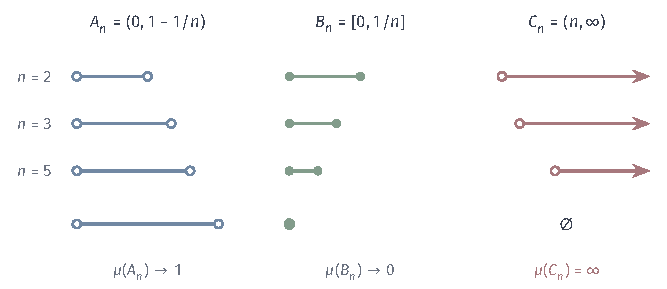
\includegraphics[width=112mm]{figures/00-shared/mathematical-preliminaries-upper/00-shared/tikz/mathematical-language-combinatorics-analysis-optimization-comprehension-additions/nested-set-limits.pdf}
  \caption{实轴上的三列嵌套集合，依次画$n=2,3,5$及最终的并集或交集，均使用勒贝格测度。左列$A_n$递增，并集为$(0,1)$；中列$B_n$递减，交集为$\{0\}$；右列$C_n=(n,\infty)$递减，交集为空，而每一项的测度仍为无穷。空心、实心端点分别表示不包含、包含；各列仅在本列内共用坐标尺度。}
  \label{fig:vol1-add-nested-set-limits}
\end{figure}
\FloatBarrier

\subsubsection{零测集与几乎处处}
\label{sec:comb-null-sets-and-completion}

集合差的测度可以描述遗漏或多出的总量。当这份总量恰为零时，函数仍可能在其中某些点取不同值，某个性质也可能在那里失效。
我们需要说明什么是零测范围、怎样表达一个性质只在零测范围内有例外，以及零测范围究竟能包含多少点。
前两个问题引出零测集和几乎处处，最后一个问题由康托尔集回答；同一删除过程还给出康托尔函数，它的增长全部集中在一个零测集上。

\paragraph{零测集}

测度为零不等于没有元素：勒贝格测度给单点赋值$0$，点本身却仍然存在。
为了用测量值而非点数描述这种范围，先给它一个名称。
\begin{definition}[零测集]
\label{def:analysis-null-set-almost-everywhere}
若$N\in\mathcal L(\mathbb R)$且$m(N)=0$，称$N$为（勒贝格）\term{零测集}（null set）。
\end{definition}
单点与所有可数点集都是零测集：它们是Borel集合，因而可测；由可数次可加性，它们的测度又不超过各单点测度之和$0$。
零测集的任意子集也是零测集：引理~\ref{lem:analysis-zero-outer-measure-measurable}已经证明，外测度为零的集合的子集都可测，单调性又使其测度为零。
因此讨论例外范围时，只要它包含在某个零测集中，就不必再单独验证它的可测性；勒贝格测度的这一性质称为完备性。

\paragraph{几乎处处}

比较两个函数时，除了判断它们是否逐点相等，还可以考察它们取值不同的位置是否都落在一个零测集中。
一般性质的例外范围也用同样的方式描述。
\begin{definition}[几乎处处]
设$E\in\mathcal L(\mathbb R)$。若存在零测集$N$，使某性质对每个$x\in E\setminus N$成立，称该性质在$E$上\term{几乎处处}（almost everywhere，简写为a.e.）成立。
\end{definition}
例如$f(0)=1$、$f(x)=0$（$x\neq0$）与恒零函数几乎处处相等，尽管它们在$0$处并不相等。
例外范围也可以是无限集，并且出现在每一小段中。
\begin{example}[有理点指示函数几乎处处为零]
在$[0,1]$上考虑$f=\mathbb I_{Q_0}$，即$x\in Q_0$时$f(x)=1$，否则$f(x)=0$。
$f$与恒零函数取值不同的点恰好组成$Q_0$，而$m(Q_0)=0$，所以$f=0$在$[0,1]$上几乎处处成立。

再看连续性。$[0,1]$中每个点的任意邻域与$[0,1]$的交都含正长度区间，因而既含$Q_0$中的点，也含无理点；$f$在其中同时取到$1$和$0$，所以$f$在$[0,1]$上处处不连续。
恒零函数则处处连续。
\end{example}

这个例子说明，“几乎处处”不表示只遗漏有限个点，也不表示每个位置附近都没有例外；几乎处处相等也不会自动保留连续性或某个指定点的取值。
后面讨论积分时，会明确哪些结论只依赖零测范围之外的取值。

若一列性质分别在零测集$N_1,N_2,\ldots$之外成立，那么它们在$\bigcup_nN_n$之外同时成立，而这个并仍是零测集。
所以可数多项几乎处处结论可以使用共同的例外范围。这一做法不能推广到不可数多项结论。
\begin{example}[不可数多项几乎处处结论不能合并]
在$[0,1]$上，对每个$t\in[0,1]$考虑性质$P_t$：$x\neq t$。它只在单点$t$处失效，所以每个$P_t$都在$[0,1]$上几乎处处成立。
若要求全部$P_t$同时成立，例外范围是$\bigcup_{t\in[0,1]}\{t\}=[0,1]$，测度为$1$；也就是说，没有任何$x\in[0,1]$满足所有$P_t$。
\end{example}

这里的并有不可数多项，可数次可加性不再适用。

\paragraph{康托尔集}
\label{sec:analysis-cantor-set}

可数集是熟悉的零测集，但零测是否意味着最多只有可数多个点，还需另行检验。
下面的康托尔集说明，点的多少与长度是否为零是两种不同的信息。

记$C_0=[0,1]$。从$C_{n-1}$的每个闭区间中删去中间的开三分之一，得到$C_n$；各层保留集合的交$C=\bigcap_{n\geq0}C_n$称为\term{康托尔集}（Cantor set）。
第$n$层$C_n$由$2^n$个长$3^{-n}$的闭区间组成，总长度为$(2/3)^n$。
按删除规则逐层归纳，这些闭区间恰为$[x_n,x_n+3^{-n}]$，其中$x_n=\sum_{j=1}^nd_j3^{-j}$、$d_j\in\{0,2\}$：从这样的区间删去中间三分之一，留下的两段正对应$d_{n+1}=0$与$d_{n+1}=2$。

下面证明$C$的测度为零，却含不可数多个点。
\begin{example}[康托尔集是不可数零测集]
\label{ex:set-measure-cantor-uncountable-null}
测度：每个$C_n$是有限个闭区间的并，因此$C$是可数个闭集的交，属于Borel集合。
由$C\subseteq C_n$和单调性，$m(C)\leq(2/3)^n$对所有$n$成立，故$m(C)=0$。

点的编码：对每条零一序列$(s_j)_{j\geq1}$，令
\[
 x=\sum_{j=1}^{\infty}\frac{2s_j}{3^j},
\]
即只用数字$0,2$的三进制数。
前$n$位确定的和$x_n=\sum_{j=1}^n2s_j3^{-j}$是$C_n$中某个闭区间的左端点，其余各位之和介于$0$与$\sum_{j>n}2\cdot3^{-j}=3^{-n}$之间，所以$x\in[x_n,x_n+3^{-n}]\subseteq C_n$。
这对每个$n$成立，故$x\in C$。

不同序列给出不同的点：若两条序列首次在第$k$位不同，对应三进制数在该位相差$2\cdot3^{-k}$，其后各位的总差至多$\sum_{j>k}2\cdot3^{-j}=3^{-k}$，所以两点之差至少为$3^{-k}>0$。

零一序列不可数：假定能列出全部序列，把第$n$条序列的第$n$位取反，得到的序列与每条已列序列都至少有一位不同，因而被遗漏。

所以$C$含不可数多个点，是不可数零测集。
\end{example}

零测例外因此能够包含不可数多个点，几乎处处的表述不能用“除去可数多个点”替代。

图~\ref{fig:analysis-process-cantor-deletion}画出上述删除过程：每一步仍有正长度，但总长度$(2/3)^n$随步数趋于零，交集却仍保留点。
\begin{figure}[!htbp]
 \centering
 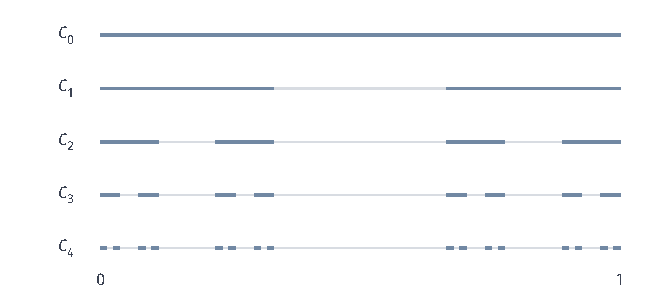
\includegraphics[width=112mm]{figures/00-shared/mathematical-preliminaries-upper/00-shared/tikz/chapter3-concept-processes/cantor-deletion.pdf}
 \caption{蓝线表示$C_0,\ldots,C_4$，每一步从上一行各闭区间中删去中间开三分之一。$C_n$由$2^n$个长度$3^{-n}$的闭区间组成，总长度为$(2/3)^n$；交集$C$的测度因此为零，但始终包含$0,1$。任何有限一行仍有正测度，不能把有限阶段当成最终零测集。}
 \label{fig:analysis-process-cantor-deletion}
\end{figure}

\paragraph{康托尔函数}
\label{sec:analysis-cantor-function}
康托尔集的长度为零，却仍可以承载函数的全部增长。下面用同一删除过程构造一个连续的非减函数：它在每个删去的区间上保持常数，因而在零测集$C$之外导数为零，却从$0$增加到$1$。

$C$中的点在每一步落在左或右保留区间，分别确定三进制表示的下一位为$0$或$2$，所以$C$中每点都有只含这两个数字的表示；示例~\ref{ex:set-measure-cantor-uncountable-null}已说明不同数字序列给出不同的点，因此这种表示唯一。
把三进制数字$0,2$分别改为二进制数字$0,1$，定义
\[
 x=\sum_{j=1}^\infty\frac{\varepsilon_j}{3^j},\qquad
 F(x)=\sum_{j=1}^\infty\frac{\varepsilon_j/2}{2^j},
 \qquad\varepsilon_j\in\{0,2\}.
\]
第二个级数由几何级数$\sum_j2^{-j}$控制，取值在$[0,1]$中；其中$x=1$取全为$2$的表示，$F(1)=1$。

$F$在$C$上不减。若$C$中两点$x<y$的三进制位首次在第$k$位不同，由示例~\ref{ex:set-measure-cantor-uncountable-null}中对首个不同位的估计，较大的$y$在该位取$2$，$x$取$0$。
于是$F(y)$在二进制第$k$位比$F(x)$多$2^{-k}$，而后续各位造成的反向差至多为$\sum_{j>k}2^{-j}=2^{-k}$，所以$F(x)\leq F(y)$。

再把$F$延拓到删去的区间上。若一个开区间在第$k$步删去，它的两端都在$C$中，三进制表示的前$k-1$位相同；左端点第$k$位为$0$而后全为$2$，右端点第$k$位为$2$而后全为$0$。
对应的二进制数分别是该位为$0$而后全为$1$、该位为$1$而后全为$0$，同一个尾和恒等式$\sum_{j>k}2^{-j}=2^{-k}$保证两值相等。
例如$1/3=0.0222\ldots_3$与$2/3=0.2000\ldots_3$都对应$1/2$。
在该开区间上把$F$定义为这个共同值，就得到整个$[0,1]$上的\term{康托尔函数}（Cantor function）。

下面验证康托尔函数的单调性、连续性与导数，并说明它的增长集中在$C$上。
\begin{example}[康托尔函数的连续性与导数]
单调与端点：$F$在$C$上不减，在每个删去区间上取两端的共同值，所以在$[0,1]$上不减，且$F(0)=0$、$F(1)=1$。

一致连续：在第$n$步的每个保留区间上，$C$中的点有相同的前$n$位三进制数字，$F$的值因而有相同的前$n$位二进制数字，都落在一个长$2^{-n}$的区间内；删去区间上的取值也在这个范围中。
所以$F$在每个第$n$步保留区间上的变化不超过$2^{-n}$。
相邻两个第$n$步保留区间之间至少隔着长$3^{-n}$的删去区间，因此两个相距小于$3^{-n}$的点之间至多涉及两个第$n$步保留区间，函数值之差不超过$2^{1-n}$。
对任意给定的误差上界，先选$n$使$2^{1-n}$小于它，再取$\delta=3^{-n}$，就得到一致连续性。

导数：$[0,1]\setminus C$是全部删去开区间的并，$F$在每个删去开区间内恒定，所以$F'=0$于$[0,1]\setminus C$。由于$m(C)=0$，$F'=0$在$[0,1]$上几乎处处成立。

不绝对连续：第$n$步的$2^n$个保留区间总长度为$(2/3)^n\to0$，但每个保留区间两端的$F$值恰好相差$2^{-n}$，端点变化的总和仍为$2^n\cdot2^{-n}=1$。
把定义~\ref{def:measurable-absolutely-continuous-function}中的误差界取为$1$：无论$\delta>0$多小，只要$(2/3)^n<\delta$，这组保留区间的总长度就小于$\delta$，端点变化之和却等于$1$，所以定义的要求不成立。
\end{example}

所以康托尔函数一致连续（因而连续）、几乎处处导数为零，全部增长$F(1)-F(0)=1$却集中在零测集$C$上。
第~\ref{sec:analysis-fundamental-calculus}节将用它说明，只知道函数连续且几乎处处可导，不能由导数的积分恢复端点变化。

\FloatBarrier

\section{一元函数的可测性和积分}
\label{sec:analysis-measurability-integration}
\label{sec:analysis-integration-average}
\label{sec:analysis-classical-integration}

第~\ref{sec:comb-set-measurement}节回答了怎样测量集合的大小。现在进一步问：函数在不同位置取不同的值时，怎样把这些值与所在范围的大小结合起来，得到一个累计量？
例如，长为$\ell$的一段区间上密度恒为$c$，总质量就是$c\ell$；密度随位置变化时，需要把这种计算推广到一般函数。
本节的自变量始终是一维实变量，有限区间$[a,b]$总设$a<b$；集合的大小始终用勒贝格测度$m$度量。

我们先沿输入区间分段取样，建立黎曼积分，并检验分割越来越细时取样结果能否稳定。
狄利克雷函数将说明，有些函数的非零取值虽然只落在零测集上，在任意短的区间上取样仍可能得到完全不同的累计。
为处理这种情形，我们利用该节的可测集合与勒贝格测度，改按函数取值划分输入：先规定哪些函数能够这样分层，再以简单函数的有限累计构造勒贝格积分。

这条路线上的几个条件各有分工：可测集合规定哪些范围允许测量，勒贝格测度给这些范围赋值，可测函数保证按取值划出的各层输入集合属于这些范围，可积条件再保证总累计有限。它们不能互相替代。

两种积分的定义及其关系明确之后，我们再研究累计函数与求导的联系、积分的运算法则、函数列与函数项级数的极限交换以及反常积分；每一步都说明所用的是哪种积分及相应的条件。

\subsection{黎曼定积分}
\label{sec:analysis-integral-definitions}
\label{sec:analysis-riemann-integral}

黎曼积分只用区间长度作权重：把输入区间切成有限个小段，研究小段越来越短时，取样累计能否趋于一个与取样无关的总量。这一构造只用到有限区间分割，还不需要一般可测集合上的积分。


\subsubsection{积分的定义}

构造从常数密度乘长度出发：先在每个小段上把函数当作常数，得到有限近似；再要求所有足够细的近似都接近同一个数。这种误差控制必须同时覆盖分割方式与取样点两种选择。


\paragraph{黎曼和}
要累计$f$在$[a,b]$上的取值，先把区间分成有限段。取
\[
 P:\quad a=x_0<x_1<\cdots<x_n=b,
\]
称$P$为一个分割，记$\Delta x_i=x_i-x_{i-1}$，$\lVert P\rVert=\max_i\Delta x_i$。细度$\lVert P\rVert$是最长小段的长度；令它趋零，要求每一段都变短，而不只是增加分割点的数量。
再在每个小区间中取样点$\xi_i\in[x_{i-1},x_i]$，用常数$f(\xi_i)$代表该段的函数值，得到
\[
 S(f,P,\xi)=\sum_{i=1}^n f(\xi_i)\Delta x_i.
\]
这称为\term{黎曼和}（Riemann sum）。若$f\geq0$，每项是一个矩形的面积；有负值时，位于横轴下方的矩形按负号计入，所以求和表示带符号的累计。
黎曼和同时依赖分割$P$与取样点$\xi$，积分的定义要求极限不受这两种选择影响。

\paragraph{黎曼积分}
区间分得越来越细时，不同取样方式所得的黎曼和仍可能不同。只有当这些取样结果都趋向同一个有限值时，才能把这个值作为函数在区间上的累计量。

\begin{definition}[黎曼积分]
\label{def:analysis-riemann-integral}
设$f:[a,b]\to\mathbb R$有界。若存在实数$A$，使对每个$\varepsilon>0$都存在$\delta>0$，当$\lVert P\rVert<\delta$时，不论怎样选取样点都有
\[
 |S(f,P,\xi)-A|<\varepsilon,
\]
则称$f$在$[a,b]$上\term{黎曼可积}（Riemann integrable），并称$A$为其\term{黎曼积分}（Riemann integral），记为$\int_a^bf(x)\,\mathrm dx$。
\end{definition}
定义中的$\delta$只依赖$\varepsilon$：只要分割足够细，无论分割点和取样点怎样选取，黎曼和都落在$A$附近。最简单的情形是常数函数$f(x)=c$，它的每个黎曼和都等于$c(b-a)$，所以积分为$c(b-a)$。对一般函数，直接检查全部取样并不方便，下一小节改用上和与下和判断共同极限是否存在。

\paragraph{定积分与积分变量}
固定被积函数和积分范围后，$\int_a^bf(x)\,\mathrm dx$是一个数，称为定积分；$a,b$分别为下限和上限，$x$为积分变量。积分变量只在积分式内部使用，换成$t$不改变结果：$\int_a^bf(x)\,\mathrm dx=\int_a^bf(t)\,\mathrm dt$。

端点还采用有向约定：$\int_b^af=-\int_a^bf$，$\int_a^af=0$。后面定义的勒贝格积分在固定范围上同样给出一个数，区间端点记号沿用这一约定，只是可积条件不同。

\subsubsection{可积性的要求}
\label{sec:analysis-integrability-requirements}

黎曼积分的定义只对有界函数提出，但有界性并不保证所有细分与取样得到共同极限。上和与下和把不同取样的可能结果夹在两个数之间，使可积性成为一个可以验证的误差条件。

\paragraph{上和与下和}
取样点可能选到小段中不同的函数值。为了同时控制全部选择，设$f$在$[a,b]$上有界，对分割$P$定义
\begin{equation}
 \begin{aligned}
 m_i&=\inf_{[x_{i-1},x_i]}f,\qquad M_i=\sup_{[x_{i-1},x_i]}f,\\
 L(f,P)&=\sum_i m_i\Delta x_i,\qquad
 U(f,P)=\sum_i M_i\Delta x_i.
 \end{aligned}
\label{eq:analysis-riemann-upper-lower-sums}
\end{equation}
$L(f,P)$称为下和，$U(f,P)$称为上和。由于$m_i\leq f(\xi_i)\leq M_i$，同一分割下的任意黎曼和都满足$L(f,P)\leq S(f,P,\xi)\leq U(f,P)$。这里用上确界和下确界而不用最大值和最小值，是因为有界函数在小段上未必取到最值。

\paragraph{Darboux判据}
加入新的分割点时，一个小段被拆成几段，每个子段上的下确界不小于原段的下确界，上确界不大于原段的上确界，所以下和不减、上和不增。任意两个分割都有公共加细，因而任意下和都不超过任意上和。于是可以定义下积分$\sup_PL(f,P)$与上积分$\inf_PU(f,P)$，并且下积分不超过上积分。

Darboux判据断言：有界函数$f$黎曼可积，当且仅当上积分与下积分相等；等价地，对每个$\varepsilon>0$存在分割$P$满足
\[
 U(f,P)-L(f,P)<\varepsilon.
\]
后两种说法的等价性直接来自定义。上下积分相等时，分别取下和、上和接近它们的两个分割，再取公共加细，即得上述小差；反之，若某个分割的上下和之差小于$\varepsilon$，上下积分之差也小于$\varepsilon$。

还须证明这一条件与黎曼积分的定义等价。先设上下和之差可以任意小。给定$\varepsilon>0$，固定一个满足$U(f,P_0)-L(f,P_0)<\varepsilon$的分割$P_0$，设它有$k$个内分割点，且$|f|\leq M$。对另一个分割$Q$，不含$P_0$分割点的小段都落在$P_0$的某一段内，可以沿用该段的上下界；跨过$P_0$分割点的小段至多$k$个，总长度至多为$k\lVert Q\rVert$，函数在其上的振幅至多为$2M$。因此
\[
 U(f,Q)-L(f,Q)\leq U(f,P_0)-L(f,P_0)+2Mk\lVert Q\rVert.
\]
令$\lVert Q\rVert$足够小，右侧便小于$2\varepsilon$。任意取样的黎曼和与上下积分的共同值都夹在$L(f,Q)$与$U(f,Q)$之间，所以二者之差小于$2\varepsilon$，这正是黎曼积分的定义。
反过来，若$f$按定义黎曼可积，取一个足够细的分割，在每个小段上分别选接近上确界和接近下确界的取样点。两组黎曼和都接近积分值，又分别接近$U(f,P)$与$L(f,P)$，所以上下和之差可以任意小。因此Darboux判据与黎曼积分的定义等价。

图~\ref{fig:analysis-process-riemann-upper-lower}显示分割加细怎样缩小上和与下和之间的差距。
\begin{figure*}[!htbp]
 \centering
 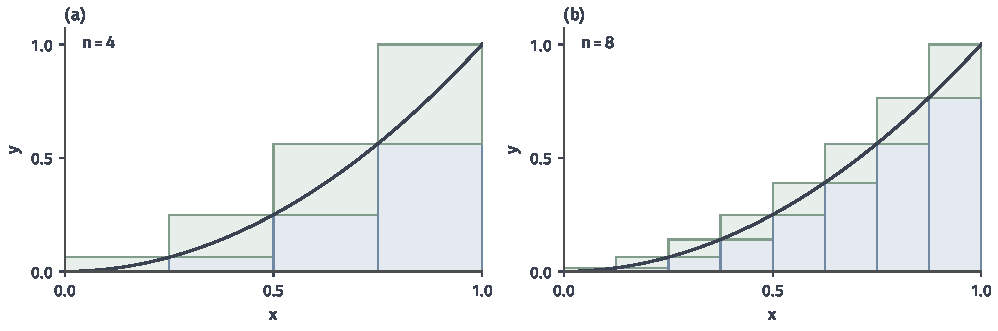
\includegraphics[width=169.0mm]{figures/00-shared/mathematical-preliminaries-upper/00-shared/matplotlib/chapter3-concept-processes/riemann-upper-lower.pdf}
 \caption{对$[0,1]$上的$f(x)=x^2$，分别等分为4段、8段。蓝色矩形累计下和，补上绿色部分得到上和，黑线为函数图像。绿色部分的总面积就是$U_n-L_n=1/n$，从$1/4$降到$1/8$；Darboux判据要求这种差能任意小，而不只是在选定的某一张图中较小。}
 \label{fig:analysis-process-riemann-upper-lower}
\end{figure*}

\paragraph{连续函数的可积性}
Darboux判据首先用于连续函数。
若$f$在$[a,b]$上连续，则由闭区间上连续函数的性质，$f$有界且一致连续。给定$\varepsilon>0$，取$\delta>0$使输入距离小于$\delta$时，输出距离小于$\varepsilon/[2(b-a)]$。对细度小于$\delta$的分割，每段上的振幅$M_i-m_i$都不超过$\varepsilon/[2(b-a)]$，所以
\[
 U(f,P)-L(f,P)=\sum_i(M_i-m_i)\Delta x_i\leq\varepsilon/2<\varepsilon.
\]
因此闭区间上的连续函数黎曼可积。一致连续性在这里给出一个对所有小段同时适用的尺度$\delta$；若只在各点分别连续，所需的段长可能随位置变化。

\paragraph{有限间断点函数的可积性}
连续性是黎曼可积的充分条件，却不是必要条件。若有界函数只在有限个点不连续，可以先用很短的区间把这些点隔离，再在其余范围上使用连续性。

设$|f|\leq M$，其中$M>0$，不连续点为$c_1,\ldots,c_k$。给定$\varepsilon>0$，用总长度小于$\varepsilon/(4M)$的有限个开区间包住这些点；函数在这些小段上的振幅至多为$2M$，所以这些小段对$U-L$的贡献不超过$\varepsilon/2$。其余部分由有限个闭区间组成，$f$在其上连续，按连续函数情形的方法加细，可使它们的贡献也小于$\varepsilon/2$。把两部分的分割点合在一起，就得到$U(f,P)-L(f,P)<\varepsilon$，所以$f$黎曼可积。
例如只有有限个跳跃的分段连续有界函数，以及把连续函数在有限个点改为其他有限值所得的函数，都属于这种情形。

\subsubsection{黎曼积分的基本性质}

Darboux判据回答了哪些函数黎曼可积。后面合并相邻区间上的累计、建立微积分基本定理时，还要用到积分关于积分区间和被积函数的基本运算；这些性质都可以直接从黎曼和与上下和得到。

\paragraph{区间可加性}
若$f$在$[a,b]$上黎曼可积，则它在每个子区间上也黎曼可积：把子区间的端点加入分割后，上下和之差中属于该子区间的部分是一些非负项之和，不超过全区间上的差，再由Darboux判据即得。
对$a\leq c\leq b$，在$[a,c]$与$[c,b]$上分别取分割与取样点，合起来就是$[a,b]$上以$c$为分割点的分割，两侧黎曼和相加恰为全区间的黎曼和。令细度趋零，得到
\[
 \int_a^bf=\int_a^cf+\int_c^bf.
\]
结合有向端点约定，这个等式对$a,b,c$的任意顺序都成立，只要涉及的区间都在可积范围内。

\paragraph{加减}
若$f,g$在$[a,b]$上黎曼可积，对同一分割与同一组取样点，有$S(f\pm g,P,\xi)=S(f,P,\xi)\pm S(g,P,\xi)$。分割足够细时右侧两项分别接近$\int_a^bf$与$\int_a^bg$，所以$f\pm g$黎曼可积，且
\[
 \int_a^b\bigl(f(x)\pm g(x)\bigr)\,\mathrm dx=\int_a^bf(x)\,\mathrm dx\pm\int_a^bg(x)\,\mathrm dx.
\]

\paragraph{数乘}
若$f$在$[a,b]$上黎曼可积，$c$为实常数，则$S(cf,P,\xi)=cS(f,P,\xi)$，与$c\int_a^bf$的误差也只乘以$|c|$，所以$cf$黎曼可积，且
\[
 \int_a^bcf(x)\,\mathrm dx=c\int_a^bf(x)\,\mathrm dx.
\]

\paragraph{上下界估计}
若常数$\alpha,\beta$满足$\alpha\leq f\leq\beta$，每个黎曼和都夹在$\alpha(b-a)$与$\beta(b-a)$之间，所以
\[
 \alpha(b-a)\leq\int_a^bf(x)\,\mathrm dx\leq\beta(b-a).
\]
特别地，$|f|\leq M$时有$|\int_a^bf|\leq M(b-a)$；端点顺序颠倒时，右侧改用区间长度$|b-a|$。

以上结论只用到有限和及其极限，不依赖微积分基本定理。后面的运算法则统一采用勒贝格积分，其线性将从简单函数的构造另行建立。

\subsubsection{黎曼积分的局限}

第~\ref{sec:analysis-integrability-requirements}节已经证明，连续函数以及只有有限个间断点的有界函数都黎曼可积，但并非任意有界函数都能这样累计。下面用有理点集构造一个反例，再用同一个集合说明黎曼可积性在函数列的逐点极限下不能保持。


\paragraph{狄利克雷函数}
黎曼可积要求各段振幅乘长度的总和能够任意小。下面的有界函数在每个小段上的振幅都等于一，缩短区间无法减小这一误差。
\begin{example}[狄利克雷函数不黎曼可积]
\label{ex:analysis-dirichlet-not-riemann}
令$Q_0=\mathbb Q\cap[0,1]$，在$[0,1]$上定义$d(x)=\mathbb I_{Q_0}(x)$，称为狄利克雷函数。
每个非退化小区间都同时含有有理数和无理数，所以对任意分割$P$，每段都有$m_i=0$、$M_i=1$，从而
\[
 L(d,P)=0,\qquad U(d,P)=1.
\]
上下和之差恒为$1$，不随分割加细而减小，Darboux判据不成立。直接看黎曼和也是如此：不论分割多细，全部选有理取样点得到黎曼和$1$，全部选无理取样点得到$0$。因此$d$在$[0,1]$上不黎曼可积。
\end{example}
这里的困难不能靠加细分割解决：误差来自每个小区间内同时存在两种取值，而不是区间不够短。

第~\ref{sec:comb-set-measurement}节已经证明$m(Q_0)=0$、$m([0,1]\setminus Q_0)=1$。若不按相邻输入分组，而把取相同函数值的输入归为一组，取值$1$对应零测集$Q_0$，取值$0$对应其余部分，所需的有限计算便是
\[
 1\cdot m(Q_0)+0\cdot m([0,1]\setminus Q_0)=0.
\]
这提示我们改变分组依据：不再只用相邻输入组成的小区间代表函数，而允许把具有同一取值的输入归为一组，即使这组输入散布在许多位置。

黎曼积分在函数列的极限下也会遇到同样的障碍。
\begin{example}[有限点指示函数递增到狄利克雷函数]
\label{ex:analysis-finite-indicators-dirichlet}
将$Q_0$列举为$\{q_1,q_2,\ldots\}$，令$d_n=\mathbb I_{\{q_1,\ldots,q_n\}}$。
每个$d_n$有界，且只在$n$个点不连续，由有限间断点的结论黎曼可积；它在每个小段上的下确界为零，下和恒为零，所以$\int_0^1d_n(x)\,\mathrm dx=0$。
另一方面，对每个$x\in[0,1]$，$d_n(x)$关于$n$单调不减：若$x=q_k$，则$n\geq k$时$d_n(x)=1$；若$x$是无理数，则$d_n(x)$恒为零。所以$d_n$逐点递增到$d$，而由示例~\ref{ex:analysis-dirichlet-not-riemann}，$d$不黎曼可积。
\end{example}
可见各项都黎曼可积，并不保证逐点极限仍黎曼可积。后面将看到，按取值分层的新累计既能处理$d$，也能在非负单调逼近下保留积分的极限。

这并不否定黎曼积分在连续函数等情形中的作用。新的构造还必须证明，在原来黎曼可积的范围内，它与已有的积分相等。

\subsection{勒贝格定积分}
\label{sec:analysis-lebesgue-definite-integral}

狄利克雷函数只取两个值，两个取值集合都可测，因此可以按“函数值乘相应集合的测度”计算。
一般函数可能取无穷多个值，需要先把取值范围分成有限档，再逐步缩小档宽、提高截断高度。
每一档对应的输入集合可能散布在许多位置，不必是一个区间。

第~\ref{sec:comb-set-measurement}节的测量结构在这里各有分工：可测集族$\mathcal L(\mathbb R)$保证各档集合经可数次集合运算后仍可测量，勒贝格测度$m$给每一档赋予大小。
还缺的是函数一侧的条件：函数划出的各档输入集合是否可测。因此先引入可测函数，再依次定义简单函数的积分和非负函数的积分，最后检查有符号累计何时有限。
以下$E$总表示$\mathcal L(\mathbb R)$中的集合，用作函数的定义域或积分范围。

\subsubsection{可测函数}
\label{sec:analysis-measurable-functions}

按取值分层之前，先要求函数满足一个资格条件：每一层的输入集合都属于可测集族。这个条件只保证各层能够测量，不保证总累计有限。


\paragraph{可测函数的定义}
可测集是输入范围中的集合；可测函数则要保证，指定输出的一段取值范围后，落入这段范围的输入仍组成可测集。
例如要计算取值大于$c$的输入占多大长度，必须先有$\{x\in E:f(x)>c\}\in\mathcal L(\mathbb R)$，才能用$m$给它赋值。

一般地，输出范围可取任意Borel集$B\subseteq\mathbb R$，分层累计依次涉及三个对象：
\[
 B\longmapsto f^{-1}(B)=\{x\in E:f(x)\in B\}
 \longmapsto m(f^{-1}(B)).
\]
测度$m$作用在输入集合$f^{-1}(B)$上，而不是作用在函数值上。可测函数要求链中的原像$f^{-1}(B)$总属于$\mathcal L(\mathbb R)$，这样第二步才有意义。
\begin{definition}[可测函数]
\label{def:analysis-measurable-function}
设$E\in\mathcal L(\mathbb R)$。函数$f:E\to\mathbb R$称为（勒贝格）\term{可测函数}（measurable function），若对每个Borel集$B\subseteq\mathbb R$，原像$f^{-1}(B)$都属于$\mathcal L(\mathbb R)$。等价地，只需对每个$a\in\mathbb R$有$\{x\in E:f(x)>a\}\in\mathcal L(\mathbb R)$。扩展实轴$[-\infty,+\infty]$的Borel结构由射线$(a,+\infty]$（$a\in\mathbb R$）生成，扩展实值函数按此结构作同样定义。
\end{definition}
阈值条件已经足够，原因有两点。第一，原像运算保持补集与可数并，所以使原像可测的输出集合$B$全体构成一个$\sigma$代数。第二，射线$(a,\infty)$生成实轴的Borel $\sigma$代数，所以这个$\sigma$代数一旦包含全部射线，就包含全部Borel集。
因此，验证可测性时通常只需检查阈值集合$\{f>a\}$，使用时则可以直接调用Borel原像条件。

例如一档取值$[u,v)$对应$\{u\leq f<v\}$，它是Borel集$[u,v)$的原像，因而可测。
对于狄利克雷函数，任一Borel集的原像只可能是$\varnothing,Q_0,[0,1]\setminus Q_0,[0,1]$之一，它们都勒贝格可测。
所以$d$虽不黎曼可积，却已经具备新构造所需的分层资格；当然，可测性本身还不能替任意函数保证积分有限。

反过来，若$A\subseteq E$不是可测集，指示函数$\mathbb I_A$就不可测，因为$\{\mathbb I_A>1/2\}=A$。
此时取值$1$所在的输入集合无法测量，“取值乘测度”的规则也就无从使用。

\paragraph{可测函数与连续函数的关系}
新的函数范围应包含原来熟悉的连续函数，同时容纳促使我们改变积分构造的狄利克雷函数。
若$E$是区间，连续函数$f:E\to\mathbb R$可测：开集的原像是$E$中的相对开集，即某个开集与$E$的交，因而是Borel集，也就勒贝格可测。反之，可测函数不必连续：狄利克雷函数的两个取值集合都勒贝格可测，所以它可测，却在每一点间断。

两者还能通过零测集上的改值联系起来。若$f$可测、$g=f$几乎处处，则对每个$a$，阈值集合$\{g>a\}$与$\{f>a\}$只相差某个零测集的子集；勒贝格测度完备，零测集的子集仍可测，所以$g$也可测。
因此只在零测集上改变取值，既不影响可测性，也不改变后面定义的积分；但这种改值可能破坏连续性，例如把零函数在$Q_0$上改为一，就得到处处不连续的狄利克雷函数。

\paragraph{可测函数的运算}
分层累计还要用于函数的加减、相乘和复合，因此应先保证这些运算不会把函数带出可测范围。
实值可测函数的和、积、绝对值、最大值与最小值仍可测。以和为例，
\[
 \{f+g>a\}=\bigcup_{q\in\mathbb Q}\bigl(\{f>q\}\cap\{g>a-q\}\bigr),
\]
右侧为可数个可测集合的并。

连续实函数$\phi$与可测函数复合所得的$\phi\circ f$仍可测。由于开集生成Borel $\sigma$代数，只需检查开集$B$的原像：$(\phi\circ f)^{-1}(B)=f^{-1}(\phi^{-1}(B))$，而$\phi^{-1}(B)$仍是开集。因而平方和绝对值可测，再由$fg=((f+g)^2-(f-g)^2)/4$得到乘积可测；最大值与最小值可由$\max\{f,g\}=(f+g+|f-g|)/2$与$\min\{f,g\}=(f+g-|f-g|)/2$得到。商在分母不为零的可测集合上可测；若要扩展到全域，需另行指定零点处的可测取值。

复合时，连续函数必须放在外层。若外层只是勒贝格可测函数，它的原像只保证是勒贝格可测集，未必是Borel集，再取内层函数的原像就可能不可测；本章不需要这种复合。扩展实值运算还要排除$\infty-\infty$等未定义形式。

\paragraph{可测函数列的极限}
后面要对函数列的极限求积分，因此还要确认极限运算不会离开可测函数的范围。
可数个可测函数的上确界、下确界可测，例如$\{\sup_nf_n>a\}=\bigcup_n\{f_n>a\}$。因此
\[
 \liminf_nf_n=\sup_N\inf_{n\geq N}f_n,\qquad
 \limsup_nf_n=\inf_N\sup_{n\geq N}f_n
\]
都可测；逐点极限存在时，它等于上、下极限，也可测。若极限只在零测集外存在，可在例外集上取值零，由零测改值的结论仍得到可测函数。
相比之下，连续函数的逐点极限可能不连续，例如$[0,1]$上$x^n$的逐点极限在$x=1$处跳跃。可测函数类对逐点极限封闭，所以用函数列逼近时不会离开这一类对象。

\subsubsection{积分的定义}

勒贝格测度给出了可测集合的大小。积分的定义分三步：先用测度计算只取有限个值的简单函数，再用简单函数从下方逼近一般非负可测函数，最后通过正负分解处理有符号函数。


\paragraph{简单函数的积分}
按取值分层累计时，最简单的情形是函数只取有限个值。只取有限个实数值的可测函数称为\term{简单函数}（simple function）。若$s$取值$a_1,\ldots,a_m$，则$E_j=\{x:s(x)=a_j\}$两两不交且可测，函数可写为$s=\sum_ja_j\mathbb I_{E_j}$。
简单函数正是“有限档”的分层：每一档是一个可测集，函数在其上取常值，该档的贡献就应为$a_jm(E_j)$。
各档两两不交，每个输入只计一次，这正是勒贝格测度的有限可加性所支持的累计方式。
下面先对非负取值定义积分，有负取值的情形稍后拆成正负两部分处理。
\begin{definition}[非负简单函数的积分]
\label{def:analysis-simple-function-integral}
设$s=\sum_{j=1}^m a_j\mathbb I_{E_j}$是$E$上的简单函数，其中$a_j\geq0$、$E_j\subseteq E$可测且两两不交，则定义
\begin{equation}
 \int_Es\,\mathrm dm=\sum_{j=1}^m a_jm(E_j).
\label{eq:analysis-simple-integral}
\end{equation}
这里约定$0\cdot\infty=0$，允许积分为$+\infty$。
\end{definition}
同一简单函数可能有不同的表示，需要确认计算结果不依赖分组方式。
把两种表示中的集合两两求交，作为公共细分，每个新块可测且函数在其上取固定值；用测度的有限可加性拆开原来的各项，两种表示便化为同一个有限和。
同一方法还证明，非负简单函数的加法、非负数乘和大小关系都与积分相容。

这个定义把集合的测度与函数的累计连接起来。对可测$A\subseteq E$，$\int_E\mathbb I_A\,\mathrm dm=m(A)$，即测量一个集合等于对它的指示函数积分；对常数$c\geq0$，则有$\int_Ec\,\mathrm dm=cm(E)$。
特别地，示例~\ref{ex:analysis-dirichlet-not-riemann}中的狄利克雷函数是简单函数，前面提示的分层计算现在就是它的积分：$\int_{[0,1]}d\,\mathrm dm=1\cdot m(Q_0)+0\cdot m([0,1]\setminus Q_0)=0$。
这个值由可测集$Q_0$及其补集的测度直接给出，计算没有把每个点的零长度逐一相加；那样的做法对不可数集合$[0,1]\setminus Q_0$并无意义。

图~\ref{fig:integral-value-layers}用同一函数比较两种分组方式。黎曼和的每个组是相邻输入组成的区间；简单函数的一档则由取值条件确定，输入集合可以分成互相分离的几段。

\begin{figure*}[htbp]
 \centering
 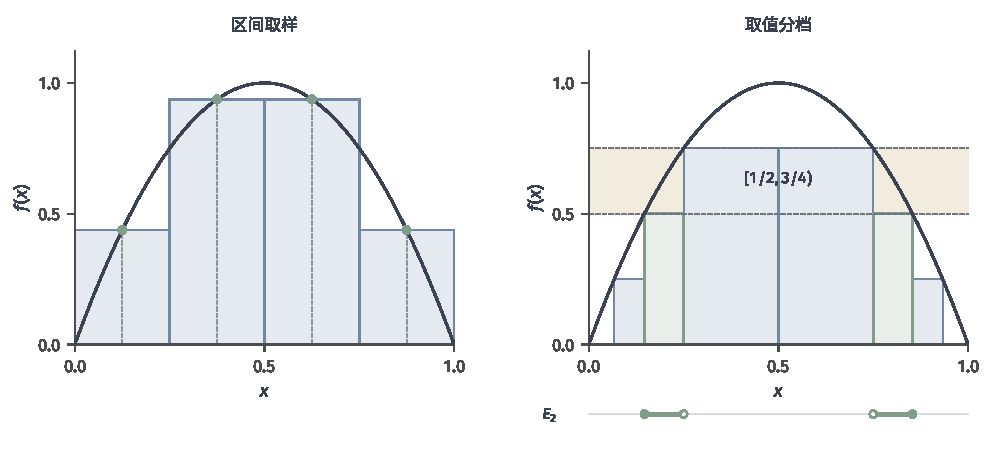
\includegraphics[width=169mm]{figures/00-shared/mathematical-preliminaries-upper/03-calculus/matplotlib/integral-value-layers/figure.pdf}
 \caption{对同一函数$f(x)=4x(1-x)$（$0\leq x\leq1$）作有限近似。左侧等分输入区间为四段，在中点取样形成黎曼和，矩形可高于或低于曲线。右侧将输出范围按$1/4$分档，在$E_j=\{x:j/4\leq f(x)<(j+1)/4\}$上取下界$a_j=j/4$；绿色标出$E_2=\{1/2\leq f<3/4\}$对应的两个输入区间，它们的总测度乘$1/2$给出这一档的贡献。下方单独画出$E_2$并标明端点。最大值处的单点不影响积分，图中略去。左侧累计为$\sum_i f(\xi_i)\Delta x_i$，右侧简单函数的累计为$\sum_j a_jm(E_j)$。勒贝格构造加细的是取值档，权重仍来自输入集合的测度。}
 \label{fig:integral-value-layers}
\end{figure*}


\paragraph{非负勒贝格积分}
一般非负可测函数可能取无穷多个值，不能直接套用有限和。但它可以由简单函数从下方逐步逼近，这为用简单函数定义一般积分提供了依据。
若只把取值舍入到网格，无界函数仍会取无穷多个网格值；若只截断高度，截断后的函数仍可能取连续多个值。因此同时做两件事：把高度截断到$n$，并把取值向下舍入到步长$2^{-n}$的网格，得到
\begin{equation}
 \begin{aligned}
 s_n(x)&=\sum_{k=0}^{n2^n-1}\frac{k}{2^n}
  \mathbb I_{\{k/2^n\leq f<(k+1)/2^n\}}(x)\\
 &\quad+n\mathbb I_{\{f\geq n\}}(x).
 \end{aligned}
\label{eq:analysis-canonical-simple-approximation}
\end{equation}
每个$s_n$只取有限个值，取值集合可测，且$0\leq s_n\leq f$。从$n$到$n+1$时网格加细、截断高度增大，所以下方近似不减。若$f(x)$有限，则$n>f(x)$以后舍入误差小于$2^{-n}$；若$f(x)=\infty$，则$s_n(x)=n$。因此$s_n\uparrow f$逐点成立，称$(s_n)$为$f$的规范简单逼近。
反过来，由第~\ref{sec:analysis-measurable-functions}节，可测函数列的逐点极限仍可测，所以非负函数可测，当且仅当它是一列非负简单函数的逐点递增极限。
这些$s_n$的积分是否趋于$f$的积分，要等定义了一般积分后，由单调收敛定理回答。

每个满足$0\leq s\leq f$的简单函数$s$都给出$f$累计的一个下界$\int_Es\,\mathrm dm$，规范简单逼近又说明这些下方函数可以逐点任意接近$f$。因此取全部这样的下界的上确界，作为$f$的累计。
\begin{definition}[非负勒贝格积分]
\label{def:analysis-nonnegative-lebesgue-integral}
若$f:E\to[0,\infty]$可测，定义
\begin{equation}
 \int_Ef\,\mathrm dm
 =\sup\left\{\int_Es\,\mathrm dm:
       s\text{为非负简单函数},\ 0\leq s\leq f\right\}.
\label{eq:analysis-nonnegative-lebesgue-integral}
\end{equation}
这称为$f$在$E$上的非负\term{勒贝格积分}（Lebesgue integral），值可为$+\infty$。
\end{definition}
上确界取遍所有下方简单函数，保留了它们能累计到的全部贡献，结果不依赖某一列特定的逼近，也不依赖取样。

对可测$A\subseteq E$，记$\int_Af\,\mathrm dm=\int_Ef\mathbb I_A\,\mathrm dm$。常写$\int_Ef(x)\,\mathrm dx$代替$\int_Ef\,\mathrm dm$；$E=[a,b]$时也写$\int_a^bf(x)\,\mathrm dx$，并沿用有向端点约定。

对具体函数，可以用区间上的阶梯函数从上下两侧夹住这个上确界。
\begin{example}[用阶梯函数计算恒等函数的积分]
\label{ex:analysis-step-functions-identity}
取$f(x)=x$，把$[0,1]$等分为$n$段，前$n-1$段取左闭右开区间，最后一段取闭区间。在第$i$段上取下界$(i-1)/n$，得到简单函数$\ell_n\leq f$；取上界$i/n$，得到简单函数$u_n\geq f$。它们的积分为
\[
 \int_{[0,1]}\ell_n\,\mathrm dm=\sum_{i=1}^n\frac{i-1}{n}\cdot\frac1n=\frac{n-1}{2n},\qquad
 \int_{[0,1]}u_n\,\mathrm dm=\sum_{i=1}^n\frac in\cdot\frac1n=\frac{n+1}{2n}.
\]
例如两段时下方积分为$1/4$，四段时为$3/8$。
由定义，$\int_{[0,1]}f\,\mathrm dm\geq\int_{[0,1]}\ell_n\,\mathrm dm$。另一方面，任一简单函数$0\leq s\leq f$也满足$s\leq u_n$，简单函数积分的单调性给出$\int s\leq\int u_n$；对$s$取上确界，得$\int_{[0,1]}f\,\mathrm dm\leq\int_{[0,1]}u_n\,\mathrm dm$。
令$n\to\infty$，两侧界都趋于$1/2$，所以$\int_{[0,1]}x\,\mathrm dm=1/2$。
\end{example}
下方阶梯只用到上确界定义中的一部分简单函数；上方阶梯则通过单调性限制了全部下方简单函数，两者合起来确定积分值。
图~\ref{fig:analysis-simple-integral}用$f(x)=x^2$展示同样的下方逼近。
\begin{figure*}[htbp]
 \centering
 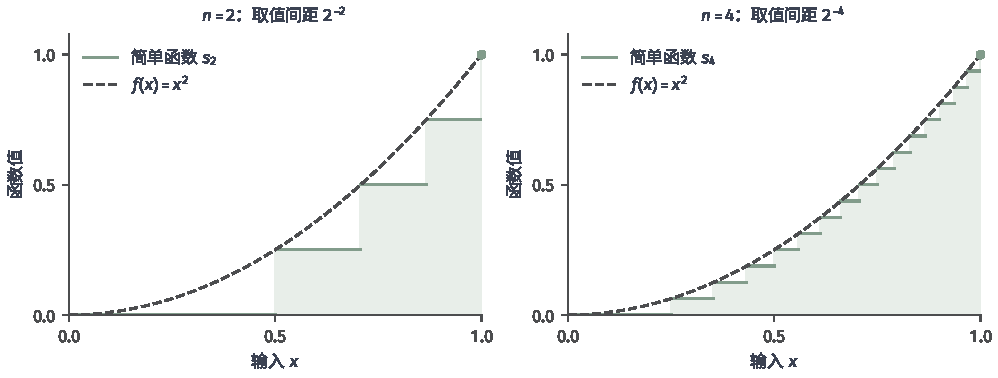
\includegraphics[width=169.0mm]{figures/00-shared/mathematical-preliminaries-upper/03-calculus/matplotlib/analysis-simple-integral/figure.pdf}
 \caption{$f(x)=x^2$在$[0,1]$上的简单函数逼近。图中将区间分别等分为两段、四段，在每段取函数下界，按高度乘长度求和；加细后下方累计增大，逼近积分$1/3$。简单函数还允许用一般可测集合代替图中的区间。}
 \label{fig:analysis-simple-integral}
\end{figure*}

\paragraph{有符号勒贝格积分}
非负函数的各部分贡献只会累加；有正负值时，还必须防止两个无穷总量相减。
对实值可测$f$，令$f^+=\max\{f,0\}$、$f^-=\max\{-f,0\}$，则$f=f^+-f^-$、$|f|=f^++f^-$，正负两部分均非负可测。
只要它们的积分不同时为无穷，就定义
\[
 \int_Ef\,\mathrm dm=\int_Ef^+\,\mathrm dm-\int_Ef^-\,\mathrm dm.
\]
两部分中恰有一个为无穷时，积分为$+\infty$或$-\infty$；两部分都为无穷时，差没有定义，也不能通过选择某种抵消次序给它指定一个有限的勒贝格积分。

\subsubsection{可积性的要求}

可测性保证各取值层可以测量，非负积分的定义给出一个确定的扩展实数值，但两者都不保证累计有限。
要使有符号积分成为有限实数，正负两部分的积分都必须有限；下面用绝对值的积分统一表述这一要求。

\begin{definition}[勒贝格可积函数]
\label{def:analysis-integrable-function}
若实值可测$f:E\to\mathbb R$满足
\begin{equation}
 \int_E|f|\,\mathrm dm<\infty,
\label{eq:analysis-absolute-integrability}
\end{equation}
则称$f$在$E$上勒贝格可积，也称\term{绝对可积}（absolutely integrable）。其有符号勒贝格积分是有限实数。
\end{definition}
由于$0\leq f^\pm\leq|f|$，凡在$f^\pm$下方的简单函数也在$|f|$下方，所以$\int_Ef^\pm\,\mathrm dm\leq\int_E|f|\,\mathrm dm<\infty$，这一定义确实给出有限的有符号积分。本节未附“黎曼”或“反常”限定的可积性均指这一绝对可积条件。

\paragraph{可积与正负部分}
可积性同时检查正、负两部分，而不只看抵消后的结果。
非负可测函数总有非负勒贝格积分，但这个值未必有限：常数一在$\mathbb R$上的积分为$+\infty$，所以它有积分值却不可积。
对有符号函数，有限积分要求正负部分的积分都有限，这与式~\eqref{eq:analysis-absolute-integrability}等价；等价性将在下一小节由非负积分的加法证明。

正负两部分都为无穷时，即使对称区间上的累计恒为零，也得不到勒贝格积分。
\begin{example}[符号函数在实轴上没有勒贝格积分]
\label{ex:analysis-sign-function-no-integral}
在$\mathbb R$上令$f=\mathbb I_{(0,\infty)}-\mathbb I_{(-\infty,0)}$，即原点处取零的符号函数。它的正部和负部分别为$f^+=\mathbb I_{(0,\infty)}$与$f^-=\mathbb I_{(-\infty,0)}$，所以
\[
 \int_{\mathbb R}f^+\,\mathrm dm=m((0,\infty))=+\infty,\qquad
 \int_{\mathbb R}f^-\,\mathrm dm=m((-\infty,0))=+\infty.
\]
两部分都为无穷，按定义$f$没有有符号勒贝格积分，当然也不可积。
另一方面，对每个$R>0$，$\int_{[-R,R]}f\,\mathrm dm=m((0,R])-m([-R,0))=R-R=0$，对称截断上的累计恒为零。
\end{example}
对称截断的零值来自正负无穷总量的成对相消，并不说明两部分有限。所以有限的有符号勒贝格积分必然来自绝对可积函数，不存在由正负无穷抵消得到的有限值。

\paragraph{有界性与可积性}
判断可积时，函数的大小与积分范围的测度必须一起考虑。
若$m(E)<\infty$且$|f|\leq M$，每个满足$0\leq s\leq|f|$的简单函数都不超过$M\mathbb I_E$，所以$\int_E|f|\,\mathrm dm\leq Mm(E)<\infty$。因此有限测度集合上的有界可测函数可积；狄利克雷函数就是这样在$[0,1]$上可积的。
在无穷测度范围上，有界性不足，实轴上的常数一已经说明这一点。
反过来，无界也未必不可积：第~\ref{sec:analysis-improper-integrals}节将算出$x^{-1/2}$在$(0,1)$上的积分等于$2$。
因此“有界”既不是可积的必要条件，也只在有限测度范围上构成充分条件。

\subsubsection{积分的性质}
\label{sec:analysis-lebesgue-basic-properties}

定义已经给出累计值，现在检查它是否保持加法、大小关系与积分范围的分拆。
先从简单函数和上确界证明非负情形，再用正负分解处理有限的有符号积分；以下的积分均关于勒贝格测度。

\paragraph{非负勒贝格积分的性质}
简单函数的积分具有线性与单调性，现在从上确界定义把这些性质推广到一般非负可测函数。证明只用前面建立的集合测度性质，所得结论为后面的累计函数和微积分基本定理提供依据。
\begin{theorem}[非负勒贝格积分的线性与单调性]
\label{lem:analysis-nonnegative-integral-properties}
设$E\in\mathcal L(\mathbb R)$，$f,g:E\to[0,\infty]$可测，$\alpha,\beta$为非负实数。
若$f\leq g$几乎处处，则$\int_Ef\,\mathrm dm\leq\int_Eg\,\mathrm dm$；
在$0\cdot\infty=0$的约定下，还有
\[
 \int_E(\alpha f+\beta g)\,\mathrm dm
 =\alpha\int_Ef\,\mathrm dm+\beta\int_Eg\,\mathrm dm.
\]
若$f=g$几乎处处，则它们的非负积分相同。
\end{theorem}
\begin{proof}
逐点单调性直接来自定义：每个简单函数$0\leq s\leq f$也满足$s\leq g$。
若$N$为零测集，简单函数在$N$上的积分为零。
对$f,g$在$E\setminus N$上相等的情形，将任意$0\leq s\leq f$在$N$上置零，
所得简单函数不超过$g$且积分未变。取上确界得$\int f\leq\int g$，反向相同；
几乎处处的单调性也可先作这项零测修改。

对加法，任取非负简单函数$s\leq f$、$t\leq g$，简单函数的有限线性给出
$\int(f+g)\geq\int s+\int t$。分别取上确界，得到
$\int(f+g)\geq\int f+\int g$。若右侧为无穷，这已给出等式；以下设右侧有限。
反向需要检查每个下方简单函数的累计。取任意非负简单函数
$u=\sum_{j=1}^m a_j\mathbb I_{E_j}\leq f+g$，其中$a_j>0$、$E_j$两两不交，
并取规范简单逼近$s_n\uparrow f$、$t_n\uparrow g$。
固定$c\in(0,1)$，令$E_{j,n}=E_j\cap\{s_n+t_n\geq ca_j\}$。
因$s_n+t_n\uparrow f+g$且$f+g\geq a_j$于$E_j$，有$E_{j,n}\uparrow E_j$。
第~\ref{sec:analysis-set-measure-continuity}节的测度递增连续性及简单函数的线性给出
\[
 \begin{aligned}
 c\int_Eu\,\mathrm dm
 &=\lim_n c\sum_j a_jm(E_{j,n})\\
 &\leq\liminf_n\left(\int_Es_n\,\mathrm dm+\int_Et_n\,\mathrm dm\right)\\
 &\leq\int_Ef\,\mathrm dm+\int_Eg\,\mathrm dm.
 \end{aligned}
\]
先令$c\uparrow1$，再对所有这样的$u$取上确界，便得到反向不等式。
正数倍的结论由$s\leq\alpha f$与$s/\alpha\leq f$在定义中的一一对应推出；
零数倍按约定处理，再与加法结合即得一般结论。
整个证明只使用简单函数的有限和、积分的上确界与集合测度的连续性，没有使用一般函数的单调收敛定理。
\end{proof}

\paragraph{有符号勒贝格积分的性质}
有正负值时，实线性要求所有参与相减的总量都有限，绝对可积性正好保证这一点。
下面同时证明可积性判别、有限线性、比较与绝对值估计。
\begin{theorem}[有符号勒贝格积分的基本性质]
\label{thm:analysis-signed-integral-properties}
设$E\in\mathcal L(\mathbb R)$，$f,g:E\to\mathbb R$可测。
函数$f$勒贝格可积，当且仅当$\int_E f^+\,\mathrm dm$与$\int_E f^-\,\mathrm dm$都有限。
若$f,g$勒贝格可积，$\alpha,\beta\in\mathbb R$，则$\alpha f+\beta g$也可积，且
\[
 \int_E(\alpha f+\beta g)\,\mathrm dm
 =\alpha\int_Ef\,\mathrm dm+\beta\int_Eg\,\mathrm dm.
\]
对上述可积的$f,g$，$f\leq g$几乎处处时有$\int_E f\,\mathrm dm\leq\int_E g\,\mathrm dm$，并且
\[
 \left|\int_Ef\,\mathrm dm\right|\leq\int_E|f|\,\mathrm dm.
\]
若$f$可积且$g=f$几乎处处，则$g$也可积，积分与$f$相同。
\end{theorem}
\begin{proof}
由$|f|=f^++f^-$及非负积分的加法，
$\int|f|=\int f^++\int f^-$，所以绝对积分有限等价于正负两项均有限。
再检查有符号积分与正负分解以外的表示是否相容。若$f=u-v$，其中$u,v$非负且可积，
则$f^+,f^-\leq u+v$，故$f$可积；非负恒等式$u+f^-=v+f^+$积分后可移去有限项，得到
$\int f=\int u-\int v$。

对可积$f,g$，$|f+g|\leq|f|+|g|$保证和可积。
将$f+g=(f^++g^+)-(f^-+g^-)$代入刚才的分解结论，再用非负加法，得到
$\int(f+g)=\int f+\int g$。正数倍沿用非负缩放，负数倍交换正负部分，零数倍直接成立，因而实线性成立。
若$f\leq g$几乎处处，可积差$g-f$的积分非负，移项即得比较关系。
定义中的正负分解与实数三角不等式给出
$|\int f|\leq\int f^++\int f^-=\int|f|$。
最后，若$f=g$几乎处处，则$g$可测；把非负积分的零测修改不变性分别用于$|f|,|g|$及正负部分，便得$g$可积且积分相同。
\end{proof}

证明中的每次移项都只移去有限值，没有通过正负无穷的抵消得到有限值。非负积分可以等于无穷，但有符号线性中的移项必须满足上述有限性条件。

\paragraph{零积分与零测例外}
非负函数没有正负抵消，积分为零应当意味着它的正值只落在零测范围内。
下面把这一判断写成等价条件，供后面比较两种积分时使用。
\begin{theorem}[非负函数的零积分判别]
\label{thm:analysis-zero-integral}
设$E\in\mathcal L(\mathbb R)$，$f:E\to[0,\infty]$可测，则
\[
 \int_Ef\,\mathrm dm=0\quad\Longleftrightarrow\quad f=0\ \text{几乎处处}.
\]
特别地，实值可测$f$满足$\int_E|f|\,\mathrm dm=0$当且仅当$f=0$几乎处处。
\end{theorem}
\begin{proof}
若积分为零，对每个正整数$k$，$f\geq k^{-1}\mathbb I_{\{f\geq1/k\}}$，故
$0\geq k^{-1}m(\{f\geq1/k\})$。这些集合都零测，而
$\{f>0\}=\bigcup_{k\geq1}\{f\geq1/k\}$，所以$f=0$几乎处处。
反之，非负积分的零测修改不变性表明$f$与零函数的积分相等。将结论用于$|f|$便得最后一条。
\end{proof}
对有正负值的$f$，仅有$\int f=0$不能推出$f=0$几乎处处，例如$f(x)=x$在$[-1,1]$上的积分为零。

\paragraph{积分范围的可加性}
函数值可以相加，积分范围也可以分拆；后者要保持的是可测集合的不交并。
下面从测度的可数可加性直接证明这一性质，不提前使用函数列的收敛定理。
\begin{theorem}[勒贝格积分的区域可加性]
\label{thm:analysis-integral-set-additivity}
设$A_n\in\mathcal L(\mathbb R)$两两不交，$A=\bigcup_{n\geq1}A_n$。
若$f:A\to[0,\infty]$可测，则
\[
 \int_Af\,\mathrm dm=\sum_{n=1}^{\infty}\int_{A_n}f\,\mathrm dm,
\]
允许等式两侧为无穷。若$f$实值且在$A$上绝对可积，同一等式成立，且右侧绝对收敛。
对可测$B,C$及在$B\cup C$上绝对可积的实值$f$，还有
\[
 \int_{B\cup C}f=\int_Bf+\int_Cf-\int_{B\cap C}f.
\]
特别地，$C\subseteq B$时有$\int_{B\setminus C}f=\int_Bf-\int_Cf$。
\end{theorem}
\begin{proof}
非负积分的有限区域加法来自指示函数恒等式与非负线性。
因此$\int_A f\geq\sum_{n=1}^N\int_{A_n}f$对每个$N$成立，取部分和的上确界得到一个方向。
反向取任意简单函数$0\leq s=\sum_{j=1}^r c_j\mathbb I_{E_j}\leq f$，其中$c_j>0$且$E_j$两两不交、均包含于$A$。
测度的可数可加性及有限和与非负级数的合并给出
\[
 \int_As\,\mathrm dm
 =\sum_{j=1}^r c_j\sum_{n\geq1}m(E_j\cap A_n)
 =\sum_{n\geq1}\int_{A_n}s\,\mathrm dm
 \leq\sum_{n\geq1}\int_{A_n}f\,\mathrm dm.
\]
对全部这样的$s$取上确界，得到反向不等式。

若$f$在$A$上绝对可积，先对$|f|$使用非负结论，得到
$\sum_n|\int_{A_n}f|\leq\sum_n\int_{A_n}|f|=\int_A|f|<\infty$。
再分别对$f^+,f^-$使用等式并相减，便得到有符号版本。
最后，将有限实线性用于
$\mathbb I_{B\cup C}+\mathbb I_{B\cap C}=\mathbb I_B+\mathbb I_C$即得容斥式，包含情形再化为差集式。
\end{proof}
非负函数的积分为无穷时，区域相加的等式仍成立，但不能把它随意改写为含$\infty-\infty$的差。

\subsubsection{与黎曼积分的关系}

新的定义既要处理原来无法累计的函数，也要与已有的数值相容。下面先证明新定义没有改变黎曼可积函数的积分值，再用不连续点的测度准确刻画哪些函数黎曼可积。


\paragraph{黎曼积分与勒贝格积分的关系}
改变累计方式之后，必须检验原来已经能够计算的积分是否得到保留。
下面把黎曼上下和看作简单函数的积分，借助可测的上下包络及其零测差证明两种积分一致。
\begin{theorem}[黎曼积分与勒贝格积分的一致性]
\label{thm:analysis-riemann-lebesgue-consistency}
设$a<b$，$f:[a,b]\to\mathbb R$有界且黎曼可积。
则$f$勒贝格可测、勒贝格可积，且
\[
 \int_a^bf(x)\,\mathrm dx\ \text{（黎曼）}
 =\int_{[a,b]}f\,\mathrm dm\ \text{（勒贝格）}.
\]
反向蕴含不成立：有界勒贝格可积函数未必黎曼可积。
\end{theorem}
\begin{proof}
设$|f|\leq M$。由Darboux判据，可取一列分割$P_n$，后一个是前一个的加细，并使$U(f,P_n)-L(f,P_n)<1/n$。
在$P_n$的每个小区间内部，令下阶梯函数$\ell_n$取该段的下确界$m_i$，上阶梯函数$u_n$取上确界$M_i$；
有限个分割点上的取值不影响积分，可以都取$f$的值。于是$\ell_n\leq f\leq u_n$，它们都是简单函数，
且$\int\ell_n\,\mathrm dm=L(f,P_n)$、$\int u_n\,\mathrm dm=U(f,P_n)$。加细使$\ell_n$逐点不减、$u_n$逐点不增。
令$\ell=\sup_n\ell_n$、$u=\inf_nu_n$。它们可测，因为$\{\ell>c\}=\bigcup_n\{\ell_n>c\}$是可数个可测集合的并，$u$同理；并且$\ell\leq f\leq u$。
非负可测函数$u-\ell$对每个$n$都满足$u-\ell\leq u_n-\ell_n$，由积分的单调性，
\[
 0\leq\int_{[a,b]}(u-\ell)\,\mathrm dm\leq U(f,P_n)-L(f,P_n)<\frac1n,
\]
所以这个积分为零。由定理~\ref{thm:analysis-zero-integral}，$\{u\neq\ell\}$是零测集。$f$只在这个零测集上可能与可测函数$\ell$不同，
而勒贝格测度完备，所以$f$勒贝格可测。有限区间上的有界可测函数绝对可积，故可使用有符号积分的比较关系。
最后，每个$n$都有$L(f,P_n)=\int\ell_n\leq\int f\leq\int u_n=U(f,P_n)$（有符号情形先给$f$加常数$M$使之非负，再用有限线性移去常数），
两端都趋于黎曼积分，所以勒贝格积分等于黎曼积分。

示例~\ref{ex:analysis-dirichlet-not-riemann}中的狄利克雷函数有界、勒贝格可积而不黎曼可积，所以反向蕴含不成立。
\end{proof}

\paragraph{黎曼可积性的测度判据}
一致性定理保留了已有的积分，却还没有回答哪些勒贝格可积函数同时黎曼可积。
下面把上下和之差与不连续点的测度联系起来，给出有界函数的准确判据。
\begin{theorem}[黎曼可积性的勒贝格判据]
\label{thm:analysis-riemann-lebesgue-criterion}
设$a<b$，$f:[a,b]\to\mathbb R$有界，$D$为$f$相对于$[a,b]$的不连续点集。
则$D$勒贝格可测，并且$f$黎曼可积当且仅当$m(D)=0$。
\end{theorem}
\begin{proof}
先用局部振幅描述不连续。记$I_r(x)=[a,b]\cap(x-r,x+r)$，定义
\[
 \omega_f(x)=\inf_{r>0}\left(\sup_{I_r(x)}f-\inf_{I_r(x)}f\right).
\]
由于$x\in I_r(x)$，$\omega_f(x)=0$恰好表示在足够小的邻域内所有取值都接近$f(x)$，因此等价于$f$在$x$连续。
对$t>0$，记$D_t=\{x:\omega_f(x)\geq t\}$。
若$\omega_f(x)<t$，存在一个邻域，其上振幅小于$t$；该邻域内的每一点都有一个包含于其中的更小邻域，所以这些点也不属于$D_t$。
因此$D_t$在$[a,b]$中闭，进而紧；$D=\bigcup_{k\geq1}D_{1/k}$为Borel集。

若$f$黎曼可积，给定$t,\varepsilon>0$，取分割$P$使$U(f,P)-L(f,P)<t\varepsilon$。
除有限个分割点外，$D_t$中的每点都位于某个振幅至少为$t$的小区间内。
这些小区间的总长度不超过$(U-L)/t<\varepsilon$，分割点自身零测，故$m(D_t)<\varepsilon$。
由$\varepsilon$任意得$m(D_t)=0$，再取可数并得到$m(D)=0$。

反之，设$m(D)=0$且$|f|\leq M$；$M=0$时结论直接成立，以下取$M>0$。
给定$\varepsilon>0$，先取$t>0$使$t(b-a)<\varepsilon/2$。
$D_t\subseteq D$为零测集，由勒贝格外测度的定义，可用总长度小于$\varepsilon/(4M)$的可数个开区间覆盖它；令$O$为这些开区间的并，则$m(O)<\varepsilon/(4M)$。
每个$x\notin D_t$都有一个相对开邻域$V_x$，其上$f$的振幅小于$t$。
$O$与这些$V_x$覆盖紧集$[a,b]$，取一个有限子覆盖。
由式~\eqref{eq:analysis-cover-uniform-radius}，这个有限覆盖存在共同半径$r>0$，使每点的相对$r$球包含在某个覆盖成员内。取$\delta=r$，长度小于$\delta$的子区间就落在以其中一点为中心的$r$球内，因此也落在某个覆盖成员内。

取细度小于$\delta$的分割。能落在某个$V_x$内的小区间，振幅小于$t$；其余小区间都包含于$O$，总长度不超过$m(O)$，振幅至多$2M$。
因此
\[
 U(f,P)-L(f,P)\leq t(b-a)+2M m(O)<\varepsilon.
\]
由Darboux判据，$f$黎曼可积。
\end{proof}
判据要求的是函数本身几乎处处连续，而不是“几乎处处等于某个连续函数”：狄利克雷函数几乎处处等于零函数，却处处不连续，因而不黎曼可积。

\subsection{不定积分和变上限积分}
\label{sec:analysis-definite-indefinite-integrals}

定积分在指定范围上给出一个数。另有两种与积分相关的对象是函数：一种是导数等于给定函数的原函数，它们组成一个函数族；另一种把定积分的上端点改为变量，得到累计函数。本小节先分别定义二者，暂不断言它们相同。

\subsubsection{不定积分}

这里暂时从累计转回求导问题：给定$f$，寻找导数为$f$的函数。这个对象先单独定义，它与积分的联系留给微积分基本定理证明。


\paragraph{原函数}
设$f$定义在区间$I$上。若可微函数$G$在$I$上满足$G'=f$，就称$G$为$f$的原函数；寻找这样的$G$称为求原函数。原函数的定义只涉及求导，还没有断言它与定积分有何关系。例如$x^2/2$是$x$在实轴上的一个原函数。

\paragraph{不定积分}
若$G_1,G_2$都是$f$在区间$I$上的原函数，则$(G_1-G_2)'=0$，由中值定理，二者在$I$上只差一个常数。因此只要$f$在$I$上有一个原函数$G$，它的全部原函数就是$G+C$，其中$C$取遍实常数；记作$\int f(x)\,\mathrm dx=G(x)+C$，称为不定积分。如果定义域由互不相连的几个区间组成，每个区间上可以取不同的常数。
不定积分表示一个函数族，不同于固定上下限后得到的数值。

\subsubsection{变上限积分}

让积分的上端点变化，就得到一个随端点变化的累计函数。它之所以有定义，是因为被积函数在每个子区间上可积；这并不等于它已经是原函数。


\paragraph{变上限积分}
若$f$在$[a,b]$上黎曼可积，令
\[
 F(x)=\int_a^xf(t)\,\mathrm dt,\qquad a\leq x\leq b.
\]
得到的$F$称为变上限积分函数，也称累计函数。$t$是积分变量，$x$是函数的自变量。例如$f(t)=1$时，$F(x)=x-a$。变上限积分是否可导、导数是否等于$f$，需要由微积分基本定理判断，不能直接从记号得出。

\paragraph{变上限勒贝格积分}
若$f$在$[a,b]$上勒贝格可积，同样定义$F(x)=\int_a^xf(t)\,\mathrm dt$，此时积分按勒贝格定义计算。可积性保证每个子区间上的积分有限，区域可加性给出$F(y)-F(x)=\int_x^yf$。对有界黎曼可积函数，由定理~\ref{thm:analysis-riemann-lebesgue-consistency}，两种积分给出相同的累计函数。对一般可积函数，累计函数是否处处或几乎处处可导，需要另外证明。

\subsubsection{原函数与累计函数的关系}

原函数从求导关系定义，累计函数从定积分构造；记号相似并不说明二者相同。若$f$连续，下一小节将证明累计函数是它的原函数；若$f$仅勒贝格可积，一般只能保证累计函数的导数几乎处处等于$f$。
例如阶跃函数$\mathbb I_{[0,\infty)}$在$[-1,1]$上可以累计，却在该区间上没有原函数。
若有可导函数$G$满足$G'=\mathbb I_{[0,\infty)}$，则$G$在$(-1,0)$内导数恒为$0$，由定理~\ref{thm:analysis-derivative-monotonicity}，$G$在$[-1,0]$上恒等于$G(0)$；在$(0,1)$内$(G(x)-x)'=0$，同理$G(x)=G(0)+x$对$x\in[0,1]$成立。于是$G$在$0$处的左导数为$0$、右导数为$1$，与$G'(0)=1$矛盾。
它的累计函数在跳跃点也不可导，示例~\ref{ex:analysis-step-primitive}将具体验证。

\subsection{微积分基本定理}
\label{sec:measurable-differentiation-recovery}
\label{sec:analysis-fundamental-calculus}

求导记录局部变化，积分记录一段范围内的累计，二者能否相互恢复，要分别回答两个问题。
第一，给定被积函数$f$，对累计函数$F(x)=\int_a^xf$求导能否恢复$f(x)$；第二，给定函数$G$，积分其导数能否得到$G(b)-G(a)$。
前者检查局部平均能否识别点值，后者检查总变化是否全部由导数记录。下面先回答第一个问题，所得的累计函数性质再用于第二个问题；黎曼与勒贝格的条件分别说明，不把“处处”与“几乎处处”的结论混在一起。

\subsubsection{积分的导数}

先给定$f$，再构造累计函数$F(x)=\int_a^xf(t)\,\mathrm dt$。
差商$(F(x+h)-F(x))/h$正是$f$在端点为$x$、$x+h$的短区间上的平均值。下面按被积函数的条件区分三种情况：黎曼可积时先在连续点恢复，局部勒贝格可积时在几乎每一点恢复，闭区间上勒贝格可积时还得到整个区间上的绝对连续性。

\paragraph{黎曼可积函数}
累计函数的增量来自一个短区间，把它除以区间长度后能否恢复点值，取决于该点附近的取值变化。
下面只在要恢复的点要求连续，不额外要求全区间连续。
\begin{theorem}[黎曼累计函数在连续点的导数]
\label{thm:analysis-riemann-primitive-derivative}
设$f$在$[a,b]$上黎曼可积，$F(x)=\int_a^xf(t)\,\mathrm dt$。
若$f$在$c\in(a,b)$处连续，则$F'(c)=f(c)$；端点连续时对应单侧导数也等于端点值。
特别地，若$f$在$[a,b]$上连续，则$F\in C^1([a,b])$且$F'=f$。
\end{theorem}
\begin{proof}
由黎曼积分的区间可加性与线性，对非零小增量$h$有
\[
 \frac{F(c+h)-F(c)}h-f(c)
 =\frac1h\int_c^{c+h}(f(t)-f(c))\,\mathrm dt.
\]
右侧绝对值不超过$c$与$c+h$之间的$\sup|f(t)-f(c)|$，连续性使它趋零。
对端点只取允许方向的$h$。若$f$处处连续，则所得导数$f$也连续，即$F\in C^1([a,b])$。
\end{proof}

由定理~\ref{thm:analysis-riemann-lebesgue-criterion}，黎曼可积函数的不连续点组成零测集，因此这里也得到$F'=f$几乎处处。这一结论不能加强为处处成立，跳跃点就是例外。
\begin{example}[阶跃函数的累计函数在跳跃点不可导]
\label{ex:analysis-step-primitive}
在$[-1,1]$上取$f=\mathbb I_{[0,1]}$。它有界且只在$0$处不连续，因而黎曼可积。累计函数为
\[
 F(x)=\int_{-1}^xf(t)\,\mathrm dt=
 \begin{cases}
  0,&-1\leq x\leq0,\\
  x,&0<x\leq1,
 \end{cases}
\]
即$F(x)=\max\{x,0\}$。在$x\neq0$处$f$连续，在端点取单侧导数，由定理~\ref{thm:analysis-riemann-primitive-derivative}，$F'(x)=f(x)$。在$x=0$处，左差商恒为$0$，右差商恒为$1$，所以$F'(0)$不存在。
\end{example}
所以累计函数只在被积函数的连续点保证恢复点值；在不连续点，导数可能不存在，也可能存在却不等于被积函数在该点的值，例如$f=\mathbb I_{\{0\}}$的累计函数恒为零，它在$0$处的导数为$0$，而$f(0)=1$。

\paragraph{局部勒贝格可积函数}
研究某一点附近的平均累计，只需要附近紧范围上的绝对积分有限，不必要求整个定义域上的积分有限。
若可测函数$f$在实轴开集$U$内的每个紧子集$K$上都满足$\int_K|f|\,\mathrm dx<\infty$，称$f$局部勒贝格可积。它只要求局部范围内绝对可积，允许$f$在整个$U$上的绝对积分为无穷。

连续点处的短区间平均趋于函数值。对局部可积函数，\term{Lebesgue微分定理}（Lebesgue differentiation theorem）将这一结论推广到几乎每一点\scite{math-hunter2011measure}。
\begin{theorem}[一维Lebesgue微分定理]
\label{thm:measurable-lebesgue-differentiation}
若$f$在开集$U\subseteq\mathbb R$上局部勒贝格可积，则对几乎每个$x\in U$，
\begin{equation}
 \lim_{r\downarrow0}\frac1{2r}\int_{x-r}^{x+r}|f(t)-f(x)|\,\mathrm dt=0.
\label{eq:measurable-lebesgue-point}
\end{equation}
从而$(2r)^{-1}\int_{x-r}^{x+r}f(t)\,\mathrm dt\to f(x)$。
\end{theorem}
满足式~\eqref{eq:measurable-lebesgue-point}的点称为勒贝格点；定理中的积分均为勒贝格积分。定理的第二条由第一条得到，因为平均值与$f(x)$之差的绝对值不超过平均绝对差。第一条的一般证明需要覆盖估计，这里引用其结论；连续点处的论证只适用于连续点，不能代替一般证明。


现在用勒贝格点计算累计函数的导数。在$U$中的一个开区间$I$上固定$x_0\in I$，令$F(x)=\int_{x_0}^xf(t)\,\mathrm dt$。
任意$x\in I$与$x_0$之间的闭区间都是$U$的紧子集，所以积分有限；这里下限不必取在定义域端点。
在$I$中$f$的每个勒贝格点$x$，区间可加性给出
\[
 \begin{aligned}
 \left|\frac{F(x+h)-F(x)}h-f(x)\right|
 &\leq\frac1{|h|}\int_{\min\{x,x+h\}}^{\max\{x,x+h\}}|f(t)-f(x)|\,\mathrm dt\\
 &\leq\frac1{|h|}\int_{x-|h|}^{x+|h|}|f(t)-f(x)|\,\mathrm dt.
 \end{aligned}
\]
最后一项是式~\eqref{eq:measurable-lebesgue-point}中平均绝对差（取$r=|h|$）的两倍，因而趋零。
所以$F'(x)=f(x)$在每个勒贝格点成立，特别地在$I$上几乎处处成立。

局部可积不能保证靠近定义域端点的累计有限。例如$f(t)=1/t$在$(0,1)$上局部可积，$\int_{1/2}^xf(t)\,\mathrm dt$对每个$x\in(0,1)$都有意义；但$\int_\varepsilon^{1/2}t^{-1}\,\mathrm dt=\log(1/(2\varepsilon))\to\infty$，下限不能改为$0$。


\paragraph{勒贝格可积函数}
若进一步要求$f$在整个闭区间$[a,b]$上勒贝格可积，则端点处的累计也有限，而且小测度集合上的积分可以统一控制。
这使累计函数在整个$[a,b]$上绝对连续；导数结论仍是前一种情形给出的勒贝格点处恢复。
\begin{theorem}[勒贝格累计函数的绝对连续性与导数]
\label{thm:analysis-lebesgue-primitive-derivative}
若$f:[a,b]\to\mathbb R$勒贝格可积，令$F(x)=\int_a^xf(t)\,\mathrm dt$，则$F$绝对连续。
在$f$的每个内点勒贝格点处，$F'(x)=f(x)$；特别地，
\begin{equation}
 F'(x)=f(x)\quad\text{几乎处处成立}.
\label{eq:measurable-indefinite-integral-derivative}
\end{equation}
这里全部使用勒贝格积分。
\end{theorem}
\begin{proof}
先控制小测度集合上的累计。给定$\varepsilon>0$，由非负积分的上确界定义，选简单函数$0\leq s\leq|f|$使
$\int(|f|-s)<\varepsilon/2$，并记$s\leq M$。
对可测$E$，积分的比较与有限加法给出
\[
 \int_E|f|\,\mathrm dm\leq M m(E)+\varepsilon/2.
\]
取$\delta>0$使$M\delta<\varepsilon/2$（$M=0$时任取$\delta$），则$m(E)<\delta$使该积分小于$\varepsilon$。
若$(a_j,b_j)$为有限个两两不交区间，$\sum_j(b_j-a_j)<\delta$，令$E$为它们的并，区域可加性与绝对值界给出
\[
 \sum_j|F(b_j)-F(a_j)|\leq\sum_j\int_{a_j}^{b_j}|f(t)|\,\mathrm dt
 =\int_E|f|\,\mathrm dm<\varepsilon.
\]
这就是$F$绝对连续；有限个端点不影响勒贝格积分。

将$f$限制到$(a,b)$，它局部勒贝格可积。前面的差商估计已经证明，在每个内点勒贝格点处$F'=f$，Lebesgue微分定理保证这些点占据几乎整个区间。
小集合估计只使用前面的积分性质，不依赖后面的函数列收敛定理。
\end{proof}
几乎处处恢复不能加强为逐点恢复：示例~\ref{ex:analysis-dirichlet-not-riemann}中狄利克雷函数的累计恒为零，导数处处为零，却在有理点与被积函数的值不同。

图~\ref{fig:analysis-process-accumulation-increment}在同一组端点下比较短区间上的面积与累计函数的增量。
\begin{figure*}[!htbp]
 \centering
 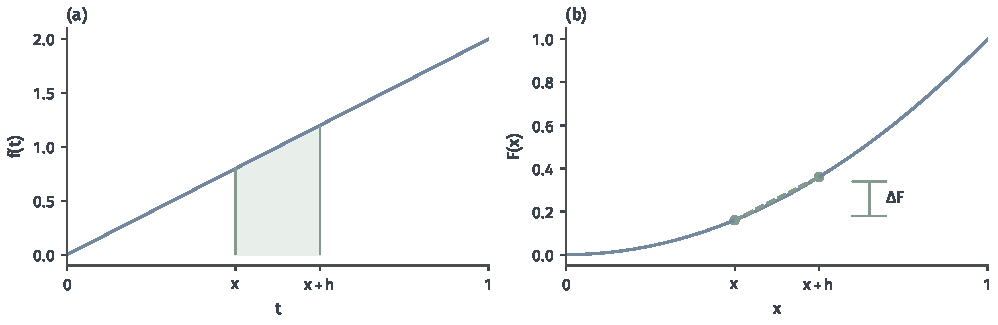
\includegraphics[width=169.0mm]{figures/00-shared/mathematical-preliminaries-upper/00-shared/matplotlib/chapter3-concept-processes/accumulation-increment.pdf}
 \caption{(a) $f(t)=2t$在$[x,x+h]$上的绿色面积。(b) $F(x)=x^2$对应的增量$\Delta F$。图取$x=0.4,h=0.2$，两者都等于$0.2$。将增量除以$h$得到短区间平均值；只有再令$h\to0$，它才趋于$f(x)$，不能把有限平均值直接当作基点导数。}
 \label{fig:analysis-process-accumulation-increment}
\end{figure*}

\subsubsection{导数的积分}

现在改为先给定$G$，再计算其导数的积分，目标是恢复端点变化。
连续导数提供最直接的充分条件，导数仅黎曼可积时仍可恢复；若只知道几乎处处可导且导数勒贝格可积，还需要对$G$的整体变化加条件。

\paragraph{黎曼可积导数的基本定理}
中值定理把每段端点增量写成导数取样值乘区间长度，因此端点恢复的关键是这些取样和能否趋于积分，而不必要求导数连续。
下面先给出黎曼可积导数的结论；连续导数是其中自动满足可积性的特例。
\begin{theorem}[黎曼可积导数的端点公式]
\label{thm:analysis-riemann-derivative-ftc}
\label{thm:analysis-newton-leibniz-continuous}
设$G$在$[a,b]$上连续、在$(a,b)$上可导，且存在黎曼可积函数$g:[a,b]\to\mathbb R$在内点满足$g=G'$。
则
\[
 \int_a^bg(x)\,\mathrm dx=G(b)-G(a).
\]
端点处给$g$指定的有限值不影响积分。特别地，若$G\in C^1([a,b])$，可取$g=G'$。
上述黎曼积分也等于相应的勒贝格积分。
\end{theorem}
\begin{proof}
对任意分割，在每个小区间上用中值定理选$\xi_i$，得到
\[
 G(b)-G(a)=\sum_i\bigl(G(x_i)-G(x_{i-1})\bigr)
 =\sum_i g(\xi_i)(x_i-x_{i-1}).
\]
$g$黎曼可积保证任意细分割的这些取样和都趋于$\int_a^bg$，所以等式成立。
改变两个端点的值仍保持黎曼可积且不改变积分。若$G\in C^1([a,b])$，连续函数的黎曼可积性保证可选$g=G'$；两种积分的一致性由定理~\ref{thm:analysis-riemann-lebesgue-consistency}给出。
\end{proof}
例如$G(x)=x^3/3$在$[0,1]$上连续可微，$G'(x)=x^2$，故$\int_0^1x^2\,\mathrm dx=1/3$，与图~\ref{fig:analysis-process-riemann-upper-lower}中上下和夹住的数值一致。
这一定理是后面计算具体积分的主要工具：先找一个原函数，再取两端的差。

\paragraph{康托尔函数的反例}
几乎处处可导只记录零测例外之外的局部变化，未必记录全部端点变化。第~\ref{sec:analysis-cantor-function}节的康托尔函数给出具体反例。
\begin{example}[康托尔函数的导数积分不恢复端点差]
\label{ex:analysis-cantor-ftc-failure}
设$F:[0,1]\to[0,1]$为康托尔函数，$C$为康托尔集。由第~\ref{sec:analysis-cantor-function}节，$F$连续、非减，$F(0)=0$、$F(1)=1$，并且在构造中删去的每个开区间上为常数。这些开区间的并就是$[0,1]\setminus C$，所以在零测集$C$之外，$F'=0$。
在导数未定义的点上令$F'=0$，所得函数几乎处处为零、勒贝格可积，于是
\[
 F(1)-F(0)=1,\qquad \int_0^1F'(x)\,\mathrm dx=0.
\]
\end{example}
所以“连续、几乎处处可导、导数可积”三项合在一起，仍不足以由导数的积分恢复函数。缺少的条件正是该节已经验证不成立的绝对连续性：康托尔函数的全部增长集中在总长度可以任意小的区间族上。

\paragraph{绝对连续函数的导数基本定理}
康托尔函数说明，连续性不能排除集中在零测集上的整体变化，因而需要更强的条件。
定义~\ref{def:measurable-absolutely-continuous-function}的绝对连续条件控制许多短区间上的总变化，能排除导数遗漏整体变化的情形。
\begin{theorem}[绝对连续函数的导数积分]
\label{thm:measurable-absolute-continuity-ftc}
若$G:[a,b]\to\mathbb R$绝对连续，则$G'$几乎处处存在，并有实值勒贝格可积函数$g$与$G'$几乎处处相等，使每个$x\in[a,b]$满足
\begin{equation}
 G(x)=G(a)+\int_a^xg(t)\,\mathrm dt.
\label{eq:measurable-absolute-continuity-representation}
\end{equation}
特别地，$G(b)-G(a)=\int_a^bG'(t)\,\mathrm dt$，其中在未定义导数的零测例外上可取值零；这些积分为勒贝格积分。
\end{theorem}
定理从绝对连续性同时推出三件事：导数几乎处处存在，导数可积，导数的积分恢复端点变化。这是测度论的基本结论，这里引用而不证明，完整证明见教材\scite{math-folland1999real}。

另一个方向已在定理~\ref{thm:analysis-lebesgue-primitive-derivative}中直接证明：勒贝格可积函数的累计必绝对连续，且几乎处处以被积函数为导数。
合看两个方向，在$[a,b]$上，$F$绝对连续当且仅当存在勒贝格可积函数$g$使
$F(x)=F(a)+\int_a^xg(t)\,\mathrm dt$，此时$F'=g$几乎处处。
所以绝对连续恰好刻画了能由导数积分恢复的函数；示例~\ref{ex:analysis-cantor-ftc-failure}则说明一致连续还不够。

\paragraph{局部Lipschitz连续函数的导数基本定理}
Lipschitz条件直接控制函数的变化，由它可以得到绝对连续，从而保证导数几乎处处存在，并在闭区间上由导数积分恢复总变化。\term{Rademacher定理}（Rademacher theorem）说明，不可导的例外点只占零测集。
\begin{theorem}[一维Rademacher定理]
\label{thm:measurable-rademacher}
若$U\subseteq\mathbb R$为开集，$f:U\to\mathbb R$局部Lipschitz连续，则$f'$在$U$内几乎处处存在且有限。若$f$在某个开区间上具有Lipschitz常数$L$，则该区间内导数存在的点满足$|f'|\leq L$。
\end{theorem}
证明先在紧区间上用绝对连续函数的基本定理得到导数存在，再用可数覆盖把局部结论合并到整个开集。
\label{sec:analysis-rademacher-proof}
\begin{proof}
紧区间上具有Lipschitz常数$L$的函数绝对连续：给定$\varepsilon>0$，取$\delta=\varepsilon/L$即可（$L=0$时函数为常数）。基本定理便保证它几乎处处可导。若$f$只在开集$U$上局部Lipschitz，可选取可数多个端点为有理数的闭区间，使其内部覆盖$U$，并使每个区间都包含在某个具有Lipschitz常数的邻域内。
各区间上的不可导点集为零测集，它们的可数并仍为零测集，故$f'$在$U$内几乎处处存在。导数存在的点处，对Lipschitz差商界取极限便给出$|f'|\leq L$。
\end{proof}
绝对值函数在原点的左右导数不同，仍符合上述几乎处处结论；定理没有把尖点处的左右导数合成一个经典导数。

在闭区间$[a,b]$上具有Lipschitz常数的函数$G$绝对连续，因此其导数除几乎处处存在之外，还满足$G(b)-G(a)=\int_a^bG'(t)\,\mathrm dt$。
康托尔函数连续、几乎处处可导且导数可积，却不满足这一公式，因此它不是Lipschitz函数。可见Lipschitz条件是一种便于验证、足以排除这类反例的条件。

\subsection{积分的运算法则}
\label{sec:analysis-integral-calculus-rules}

从这里起，本章后续的积分一律采用勒贝格积分；“可积”指绝对值的积分有限，非负函数的积分则允许为无穷。
前面已经证明积分的基本性质，现在说明怎样用它们计算函数的加减、范围的分拆，以及换元积分与分部积分。
以下$E,A,B$均为可测集，积分关于勒贝格测度。

\subsubsection{积分的基本运算}

函数相加与积分范围相加是不同的操作，分别由线性和区域可加性保证。
计算时先检查可测性及绝对可积性，再使用相应的等式；正负无穷不能通过移项抵消。

\paragraph{和的积分}
在同一可测集$E$上，若实值函数$f,g$均可积，则$|f+g|\leq|f|+|g|$保证$f+g$可积。
定理~\ref{thm:analysis-signed-integral-properties}给出
\[
 \int_E(f+g)\,\mathrm dm=\int_Ef\,\mathrm dm+\int_Eg\,\mathrm dm.
\]
反过来，同一范围上的两个有限积分也可以合并为和的积分。

\paragraph{差的积分}
两个可积函数的差仍可积，因为$|f-g|\leq|f|+|g|$。同一线性定理给出
\[
 \int_E(f-g)\,\mathrm dm=\int_Ef\,\mathrm dm-\int_Eg\,\mathrm dm.
\]
这里两项都是有限实数，不涉及正负无穷的相减。

\paragraph{数乘的积分}
把被积函数乘以固定实数$c$，积分也乘以$c$。若$f$可积，则$cf$可积，且
\[
 \int_Ecf\,\mathrm dm=c\int_Ef\,\mathrm dm.
\]
这仍是定理~\ref{thm:analysis-signed-integral-properties}的特例；$c=0$时两侧都为零。

\paragraph{积的积分}
乘积需要另行检查可积性，不能直接套用线性。若$f$可积、$g$可测且$|g|\leq M$几乎处处，其中$M$为有限常数，则$|fg|\leq M|f|$保证$fg$可积。
但即使$f,g,fg$都可积，也不能把乘积的积分拆成两个积分相乘：例如在$[0,1]$上取$f(x)=g(x)=x$，则$\int_0^1fg=1/3$，而$(\int_0^1f)(\int_0^1g)=1/4$。

\paragraph{不交范围的积分}
同一函数在不同范围上的累计，可以用区域可加性分拆。
若$A\cap B=\varnothing$，且$f$在$A\cup B$上可积，则定理~\ref{thm:analysis-integral-set-additivity}给出
\[
 \int_{A\cup B}f\,\mathrm dm=\int_Af\,\mathrm dm+\int_Bf\,\mathrm dm.
\]
这与“和的积分”不同：这里改变的是积分范围，被积函数没有相加。取$A=[a,c]$、$B=(c,b]$，便得到区间记号下的$\int_a^bf=\int_a^cf+\int_c^bf$。

\paragraph{重叠范围的积分}
若两个范围重叠，分别累计会把交集计算两次，需要减去一次。
对在$A\cup B$上可积的$f$，有
\[
 \int_{A\cup B}f\,\mathrm dm
 =\int_Af\,\mathrm dm+\int_Bf\,\mathrm dm-\int_{A\cap B}f\,\mathrm dm.
\]
将$A\cup B$拆成$A\setminus B$、$A\cap B$、$B\setminus A$三个不交部分，再用区域可加性即可得到此式。

\paragraph{差集上的积分}
从可测范围$A$中去掉可测子集$B\subseteq A$时，去掉的累计量正是$B$上的积分。
若$f$在$A$上可积，由$A=(A\setminus B)\cup B$的不交分拆，得到
\[
 \int_{A\setminus B}f\,\mathrm dm=\int_Af\,\mathrm dm-\int_Bf\,\mathrm dm.
\]

\paragraph{积分的比较}
被积函数几乎处处的大小关系可以传给积分。若$f,g$可积且$f\leq g$几乎处处，则
\[
 \int_Ef\,\mathrm dm\leq\int_Eg\,\mathrm dm.
\]
这是因为$g-f$几乎处处非负且可积，其积分非负，再由差的积分公式移项即可。

\paragraph{积分的绝对值界}
累计中的正负抵消不会超过绝对值的累计。由$-|f|\leq f\leq|f|$及积分的比较得到
\[
 \left|\int_Ef\,\mathrm dm\right|\leq\int_E|f|\,\mathrm dm.
\]
此处$f$可积，所以不等式两侧均有限。

\paragraph{积分的误差估计}
将绝对值界用于两个可积函数之差，就能控制积分结果的误差：
\[
 \left|\int_Ef\,\mathrm dm-\int_Eg\,\mathrm dm\right|
 \leq\int_E|f-g|\,\mathrm dm.
\]
若进一步有$m(E)<\infty$且$|f-g|\leq\eta$几乎处处，则右侧不超过$\eta\,m(E)$。
后面讨论极限与积分时，将用这一估计把函数的共同误差转成积分误差。

\subsubsection{换元积分法}
\label{sec:analysis-coordinate-change-integral-applications}

变量替换既改变函数的表达，也改变输入集合的长度，导数的绝对值负责一维长度的缩放。
下面先给出一一对应换元的一般结论，再说明计算中常用的端点写法，最后用几个例子展示完整步骤。

\paragraph{可测函数的换元公式}
对非负函数，换元要保留全部累计；对有符号函数，还需保证正负部分都有限。
下面用微分同胚条件同时控制可逆性、可测性与局部长度变化。
\begin{theorem}[一维勒贝格积分的换元公式]
\label{thm:analysis-lebesgue-change-variables}
设$I,J\subseteq\mathbb R$为开区间，$T:I\to J$是$C^1$微分同胚，即$T$双射且$T,T^{-1}$连续可微。
对非负勒贝格可测$g:J\to[0,\infty]$，有
\[
 \int_Jg(u)\,\mathrm du=\int_Ig(T(x))|T'(x)|\,\mathrm dx,
\]
允许两边为无穷。若$g:J\to\mathbb R$可测，则$g$在$J$上可积当且仅当$g\circ T\,|T'|$在$I$上可积，此时同一等式给出有限积分值。
\end{theorem}
直观上，$T$把输入中长为$\Delta x$的小区间映成长约$|T'(x)|\Delta x$的小区间，因子$|T'(x)|$记录这种长度缩放。
一般换元定理的证明先把这种局部长度关系推广到可测集合，再经简单函数及单调逼近推广到非负函数；这里引用这一结论\scite{math-folland1999real}。
有符号版本则先对$|g|$换元，确认两侧同时绝对可积，再分别对正负部分换元。
由于单点的测度为零，$I,J$取开区间还是闭区间不影响积分值。

\paragraph{端点形式的换元}
定理中的等式不带方向：右侧乘$|T'|$，左侧按像区间从左到右累计。计算时更常写成端点形式，不必先判断$T$是递增还是递减。
设$T$在开区间$(a,b)$上是$C^1$微分同胚，并连续延拓到两端，$g$在像区间上非负可测或可积。微分同胚的导数处处非零（否则反函数在对应点不可导），又是连续函数，所以不变号，$T$严格单调。
若$T$递增，则$|T'|=T'$，像区间从$T(a)$到$T(b)$，定理直接给出
\[
 \int_{T(a)}^{T(b)}g(u)\,\mathrm du=\int_a^bg(T(x))T'(x)\,\mathrm dx.
\]
若$T$递减，则$|T'|=-T'$，像区间从$T(b)$到$T(a)$，定理给出$\int_{T(b)}^{T(a)}g(u)\,\mathrm du=-\int_a^bg(T(x))T'(x)\,\mathrm dx$；按有向端点约定把左侧改写为$-\int_{T(a)}^{T(b)}g$，两边的负号抵消，得到与递增情形完全相同的式子。
因此端点形式对两种单调方向统一成立：导数$T'$的符号与端点的先后共同记录了方向。

\paragraph{换元的计算示例}
下面三个例子依次检验递增换元、递减换元，以及用三角函数消去根式的换元。每个例子都先核对微分同胚条件，再使用端点形式。
\begin{example}[用递增换元计算指数型积分]
计算$\int_0^12xe^{x^2}\,\mathrm dx$。被积函数形如$g(T(x))T'(x)$，其中$T(x)=x^2$、$g(u)=e^u$。
在开区间$(0,1)$上，$T'(x)=2x>0$，反函数$T^{-1}(u)=\sqrt u$在$(0,1)$上连续可微，所以$T:(0,1)\to(0,1)$是$C^1$微分同胚。
注意$T'(0)=0$，$T$不能在包含$0$的开区间上作为微分同胚；这里只在$(0,1)$上换元，端点的单点不影响积分。
端点形式给出
\[
 \int_0^12xe^{x^2}\,\mathrm dx=\int_{T(0)}^{T(1)}e^u\,\mathrm du=\int_0^1e^u\,\mathrm du.
\]
最后用定理~\ref{thm:analysis-riemann-derivative-ftc}，取原函数$e^u$，得到$e^1-e^0=e-1$。
\end{example}

导数为负时，端点的先后顺序会颠倒，端点形式自动处理由此产生的符号。
\begin{example}[用递减换元计算三角函数积分]
计算$\int_0^{\pi/2}\sin x\cos^2x\,\mathrm dx$。取$T(x)=\cos x$，它在$(0,\pi/2)$上满足$T'(x)=-\sin x<0$，是到$(0,1)$的递减$C^1$微分同胚，反函数$\arccos$在$(0,1)$上连续可微。
按端点形式，
\[
 \int_0^{\pi/2}\cos^2x\,(-\sin x)\,\mathrm dx=\int_{T(0)}^{T(\pi/2)}u^2\,\mathrm du=\int_1^0u^2\,\mathrm du=-\frac13,
\]
所以$\int_0^{\pi/2}\sin x\cos^2x\,\mathrm dx=1/3$。
若直接使用定理的无方向形式，则$|T'(x)|=\sin x$，原积分等于$\int_{(0,1)}u^2\,\mathrm du=1/3$，结果相同。
\end{example}
两种写法的差别只在方向记在哪里：端点形式记在端点的先后中，无方向形式记在$|T'|$中。

换元还可以把不易直接找原函数的积分化为容易计算的形式。
\begin{example}[用正弦换元计算四分之一单位圆的面积]
单位圆在第一象限部分的面积是
\[
 \int_0^1\sqrt{1-x^2}\,\mathrm dx.
\]
令$x=T(\theta)=\sin\theta$，则$T:(0,\pi/2)\to(0,1)$递增，$T'(\theta)=\cos\theta>0$，反函数$\arcsin$在$(0,1)$上连续可微。
在$(0,\pi/2)$上$\cos\theta>0$，所以$\sqrt{1-\sin^2\theta}=\cos\theta$，从而
\[
 \int_0^1\sqrt{1-x^2}\,\mathrm dx
 =\int_0^{\pi/2}\sqrt{1-\sin^2\theta}\,\cos\theta\,\mathrm d\theta
 =\int_0^{\pi/2}\cos^2\theta\,\mathrm d\theta.
\]
由$\cos^2\theta=(1+\cos2\theta)/2$，原函数可取$\theta/2+\sin(2\theta)/4$，代入两端得到$\pi/4$。
\end{example}
这里换元的方向是把原积分写成定理右侧的形式：先确定新旧变量的对应及导数，再化简被积函数；开方时必须用到$\cos\theta$在所取区间上的符号。

\subsubsection{分部积分法}
\label{sec:analysis-integration-remainders}

乘积的导数$(uv)'=u'v+uv'$含有两项。对它积分并使用绝对连续函数的端点恢复公式，就能把其中一项的积分移到等式另一侧。
下面直接使用绝对连续条件；连续可微函数是其特例。

\paragraph{分部积分公式}
绝对连续保证导数几乎处处存在、可积且记录全部增量，因此可以对乘积的求导公式积分。
只知道几乎处处可导仍不充分，示例~\ref{ex:analysis-cantor-ftc-failure}已说明这一差别。
\begin{theorem}[勒贝格积分的分部积分公式]
\label{thm:analysis-lebesgue-integration-by-parts}
若$u,v:[a,b]\to\mathbb R$绝对连续，则$uv$绝对连续，$uv'$与$u'v$可积，且
\begin{equation}
 \int_a^bu(x)v'(x)\,\mathrm dx
 =[u(x)v(x)]_a^b-\int_a^bu'(x)v(x)\,\mathrm dx.
\label{eq:analysis-integration-by-parts}
\end{equation}
导数在零测例外上的可测有限取值不影响结果。
\end{theorem}
\begin{proof}
$u,v$连续且有界，导数可积，所以$uv'$与$u'v$可积。
对有限个两两不交区间，有
\[
 \begin{aligned}
 \sum_j|u(b_j)v(b_j)-u(a_j)v(a_j)|
 &\leq\|u\|_\infty\sum_j|v(b_j)-v(a_j)|\\
 &\quad+\|v\|_\infty\sum_j|u(b_j)-u(a_j)|.
 \end{aligned}
\]
两因子的绝对连续性使右侧随区间总长度趋零，故$uv$绝对连续。
在两导数都存在的点，$(uv)'=u'v+uv'$；将绝对连续函数的端点恢复定理用于$uv$，再用有限线性移项，便得公式。
\end{proof}
使用公式时，要把被积函数拆成一个因子$u$与另一个因子的导数$v'$：求导后变简单的因子取作$u$，容易找到原函数的因子取作$v'$。

\paragraph{分部积分的计算示例}
下面三个例子分别说明怎样选取$u$与$v'$：让多项式因子求导降次，把单个因子看成与常数一的乘积，以及选择不当会使积分变复杂。
\begin{example}[多项式乘指数函数的分部积分]
计算$\int_0^1xe^x\,\mathrm dx$。取$u(x)=x$、$v'(x)=e^x$，则$u'(x)=1$，可取$v(x)=e^x$；两者都在$[0,1]$上连续可微，因而绝对连续。公式给出
\[
 \int_0^1xe^x\,\mathrm dx=[xe^x]_0^1-\int_0^1e^x\,\mathrm dx
 =(e-0)-(e-1)=1.
\]
\end{example}
这里$x$求导后变成常数，剩下的积分可以直接由原函数计算。

被积函数只有一个因子时，可以把常数一当作另一个因子。
\begin{example}[把对数函数看成与常数一的乘积]
计算$\int_1^e\log x\,\mathrm dx$。把被积函数写成$\log x\cdot1$：取$u(x)=\log x$、$v'(x)=1$，则$u'(x)=1/x$，可取$v(x)=x$；两者都在$[1,e]$上连续可微。于是
\[
 \int_1^e\log x\,\mathrm dx=[x\log x]_1^e-\int_1^e\frac1x\cdot x\,\mathrm dx
 =e-(e-1)=1.
\]
\end{example}
对数的导数是有理函数，分部积分正好消去了难以直接积分的对数。

因子的分配也可能使计算变繁，下面的例子比较两种选法。
\begin{example}[因子的分配决定计算是否简化]
计算$\int_0^\pi x\sin x\,\mathrm dx$。取$u(x)=x$、$v'(x)=\sin x$，则$u'(x)=1$，可取$v(x)=-\cos x$，于是
\[
 \int_0^\pi x\sin x\,\mathrm dx=[-x\cos x]_0^\pi+\int_0^\pi\cos x\,\mathrm dx
 =\pi+[\sin x]_0^\pi=\pi.
\]
若反过来取$u=\sin x$、$v'=x$，则$v=x^2/2$，剩下的积分变为$\int_0^\pi x^2\cos x/2\,\mathrm dx$，比原积分更复杂。
\end{example}
在无穷区间上使用公式时，先对有限截断应用公式，再分别核查边界项的极限以及两个被积项的绝对可积性，不能无故删除端点项。

\paragraph{Taylor公式的积分余项}
分部积分的一个重要应用，是把Taylor公式中的余项写成一个确定的积分。
第~\ref{sec:analysis-taylor-approximation}节的Lagrange余项$f^{(r+1)}(\xi)h^{r+1}/(r+1)!$中，$\xi$只知道位于两端之间，具体位置未知。
若$f^{(r+1)}$连续，可以从端点公式$f(x_0+h)-f(x_0)=\int_{x_0}^{x_0+h}f'(t)\,\mathrm dt$出发，每做一次分部积分就从积分中分出Taylor多项式的一项；剩下的积分就是余项本身，不含未知点，可以直接计算或估计。

设$f$在包含以$x_0$、$x_0+h$为端点的闭区间的某个开区间上$r+1$阶连续可微，其中$r$为非负整数。为了同时处理正、负$h$，令$\phi(t)=f(x_0+th)$，$t\in[0,1]$；链式法则给出$\phi^{(k)}(t)=h^kf^{(k)}(x_0+th)$。
第一步由黎曼可积导数的端点公式得到
\[
 \phi(1)-\phi(0)=\int_0^1\phi'(t)\,\mathrm dt.
\]
对$k\geq1$，在
$\int_0^1\frac{(1-t)^{k-1}}{(k-1)!}\phi^{(k)}(t)\,\mathrm dt$中取$u=\phi^{(k)}$、$v=-(1-t)^k/k!$，则$v'=(1-t)^{k-1}/(k-1)!$，而$v(1)=0$、$v(0)=-1/k!$。分部积分给出
\[
 \int_0^1\frac{(1-t)^{k-1}}{(k-1)!}\phi^{(k)}(t)\,\mathrm dt
 =\frac{\phi^{(k)}(0)}{k!}
 +\int_0^1\frac{(1-t)^k}{k!}\phi^{(k+1)}(t)\,\mathrm dt.
\]
从$k=1$用到$k=r$，每一步分出一项$\phi^{(k)}(0)/k!=f^{(k)}(x_0)h^k/k!$，便得
\begin{equation}
 f(x_0+h)=\sum_{k=0}^r\frac{f^{(k)}(x_0)}{k!}h^k
 +\frac{h^{r+1}}{r!}
   \int_0^1(1-t)^r f^{(r+1)}(x_0+th)\,\mathrm dt.
\label{eq:analysis-taylor-integral-remainder}
\end{equation}
最后一项称为Taylor公式的积分余项。这里的余项是勒贝格积分，$f^{(r+1)}$连续保证被积函数在$[0,1]$上可积。
若$|f^{(r+1)}|\leq M$，积分权重$(1-t)^r/r!$的总量为$1/(r+1)!$，故余项不超过$M|h|^{r+1}/(r+1)!$，与Lagrange余项的估计一致。

积分余项不含未知点，对具体函数可以直接算出或夹逼。先看三阶导数为常数的立方函数。
\begin{example}[立方函数的积分余项]
取$f(x)=x^3-3x$、$r=2$。由于$f'''\equiv6$，对任意$x_0$和$h$，积分余项为
\[
 \frac{h^3}{2!}\int_0^1 6(1-t)^2\,\mathrm dt=\frac{h^3}{2}\cdot6\cdot\frac13=h^3.
\]
这与第~\ref{sec:analysis-taylor-approximation}节中$x_0=1/2$处的完整展开相同：三阶Taylor多项式之外没有剩余项，二阶多项式的误差恰为$h^3$。
\end{example}

被积函数不是常数时，可以用它的上下界夹住余项，得到截断误差的范围。
\begin{example}[用积分余项估计$e$]
取$f(x)=e^x$、$x_0=0$、$h=1$。各阶导数都是$e^x$，式~\eqref{eq:analysis-taylor-integral-remainder}给出
\[
 e=\sum_{k=0}^r\frac1{k!}+\frac1{r!}\int_0^1(1-t)^re^t\,\mathrm dt.
\]
由$1\leq e^t\leq e$及$\int_0^1(1-t)^r\,\mathrm dt=1/(r+1)$，余项介于$1/(r+1)!$与$e/(r+1)!$之间。
例如$r=3$时，三阶Taylor多项式在$h=1$处的值为$1+1+1/2+1/6=8/3\approx2.6667$，余项$e-8/3\approx0.0516$，确实落在$1/24\approx0.0417$与$e/24\approx0.1133$之间。
\end{example}



\subsection{函数列的极限}
\label{sec:measurable-convergence-and-integrals}
\label{sec:analysis-limit-integral-interchange}
\label{sec:analysis-function-convergence-essential-bounds}

设一列函数$f_n$趋于$f$。仅知道每个位置的函数值趋近，还不能判断极限函数是否连续、是否可微，也不能判断积分的极限是否等于极限函数的积分。
这三个问题控制的对象不同：连续性比较邻近输入的函数值，微分比较差商，积分比较全部范围上的累计。
下面先明确收敛方式，再分别回答极限与连续、极限与微分、极限与积分的关系；本小节涉及的积分全部为勒贝格积分。

\subsubsection{函数列的收敛方式、判别与关系}
\label{sec:analysis-convergence-mode-relations}

逐点收敛允许每个输入单独选择稳定时刻，一致收敛要求同一个下标控制全部输入，几乎处处收敛则允许在一个固定的零测范围上例外。
先区分这些条件，后面才能说明哪种控制足以保持哪种性质。

\paragraph{点态收敛}
固定一个输入以后，比较的只是一列实数。这里不需要函数可微或可积，函数值按实数的绝对值比较。
\begin{definition}[点态收敛]
\label{def:analysis-pointwise-almost-everywhere-convergence}
设$X\subseteq\mathbb R$，$f_n,f:X\to\mathbb{R}$。若
\[
 \begin{gathered}
  \forall x\in X,\quad
  \forall\varepsilon>0,\quad
  \exists N=N(x,\varepsilon)\in\mathbb N,\\
  \forall n\geq N,\quad
  |f_n(x)-f(x)|<\varepsilon,
 \end{gathered}
\]
即对每个$x$都有$\lim_n f_n(x)=f(x)$，称$f_n$点态收敛到$f$。点态收敛也称逐点收敛（pointwise convergence）。
\end{definition}
固定$x$以后，点态收敛就是已经定义的数列收敛；不同位置可以需要不同的起始下标。

\paragraph{点态收敛的判据}
若还不知道极限函数，可以对每个固定输入使用实数列的柯西收敛准则。
这时各输入仍可各自选择尾部起点，不要求同一个下标适用于全部输入。
\begin{theorem}[函数列点态收敛的柯西判据]
\label{thm:analysis-pointwise-cauchy-criterion}
设$X$非空，$f_n:X\to\mathbb R$。存在$f:X\to\mathbb R$使$f_n$点态收敛到$f$，当且仅当
\[
 \begin{gathered}
 \forall x\in X,\quad\forall\varepsilon>0,\quad
 \exists N=N(x,\varepsilon)\in\mathbb N,\\
 \forall m,n\geq N,\quad |f_m(x)-f_n(x)|<\varepsilon.
 \end{gathered}
\]
\end{theorem}
\begin{proof}
固定$x$，若$f_n(x)$收敛，则实数列的柯西准则给出该条件。
反之，条件使每个$(f_n(x))_n$都是实数柯西列，故都有有限极限；定义$f(x)=\lim_nf_n(x)$，便得到所需的点态极限函数。
\end{proof}

\paragraph{一致收敛}
即使每个输入处的误差最终都很小，开始稳定的时刻仍可能依赖输入。
若希望选定一个下标后就同时控制全部输入，需要更强的一致条件。

\begin{definition}[函数列的一致收敛]
\label{def:analysis-uniform-convergence}
设$X\subseteq\mathbb R$非空，$f_n,f:X\to\mathbb R$。若
\[
  \forall\varepsilon>0,\quad
  \exists N=N(\varepsilon)\in\mathbb N,\quad
  \forall x\in X,\quad
  \forall n\geq N,\quad
  |f_n(x)-f(x)|<\varepsilon,
\]
就称$f_n$在$X$上一致收敛到$f$。等价地，
\begin{equation}
  \lVert f_n-f\rVert_{\infty}
  :=
  \sup_{x\in X}|f_n(x)-f(x)|
  \longrightarrow0.
\label{eq:analysis-uniform-convergence}
\end{equation}
这里的上确界检查全部输入，不排除任何位置；对一般函数，它可能等于$+\infty$，一致收敛要求这些误差最终有限并趋于零。
\end{definition}
两个定义只交换了“$\forall x$”与“$\exists N$”的次序：点态收敛先固定输入再选$N(x,\varepsilon)$，一致收敛先选$N(\varepsilon)$，再要求它适用于全部输入。
在图形上，以极限$f$为中心画出上下宽$\varepsilon$的误差带：一致收敛要求从某个下标起，$f_n$的整个图形都落在带内；点态收敛只要求每条竖线$x=x_0$上的点$f_n(x_0)$最终进入带内，进入的时刻可以随$x_0$改变。

图~\ref{fig:analysis-process-convergence-modes}用两个具体函数列比较这一差别，误差带都取$\varepsilon=0.12$。
(a)中$g_n(x)=x/n$在$[0,1]$上的最大误差为$1/n$，从$N=9$起整个图形都在带内，同一个$N$对全部输入适用。
(b)中$f_n(x)=x^n$在$[0,1)$上点态收敛到$0$：在$x_1=0.5$处从$n=4$起进入带内，在$x_2=0.9$处要等到$n=21$；输入越靠近$1$，所需的$N$越大。
每条$f_n$都在$x=\varepsilon^{1/n}<1$处离开误差带；由于$\sup_{[0,1)}x^n=1$，没有一个$N$能对全部输入同时适用。
\begin{figure*}[!htbp]
 \centering
 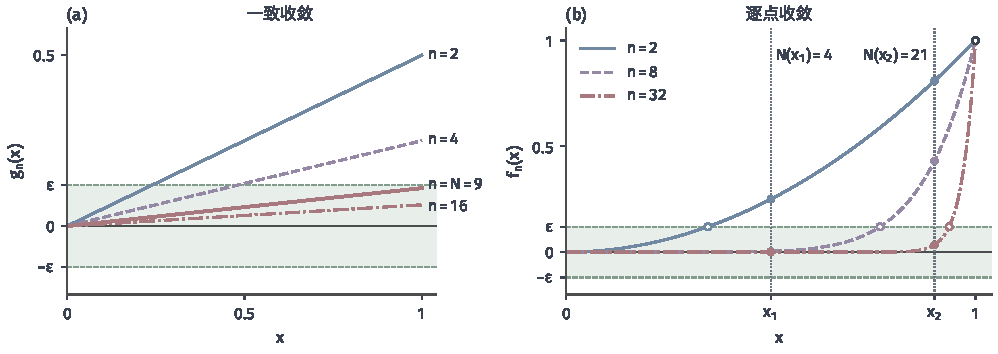
\includegraphics[width=169.0mm]{figures/00-shared/mathematical-preliminaries-upper/00-shared/matplotlib/chapter3-concept-processes/convergence-modes.pdf}
 \caption{函数列的两种收敛方式，绿色带为极限$0$附近宽$\varepsilon=0.12$的误差带。(a)一致收敛：$g_n(x)=x/n$在$[0,1]$上的最大误差为$1/n$，$n=2,4$时图形超出误差带，从$N=9$起（图中加粗）整个图形都在带内。(b)逐点收敛：$f_n(x)=x^n$在$[0,1)$上趋于$0$，图绘$n=2,8,32$。竖虚线$x_1=0.5$、$x_2=0.9$上的实心点是各曲线在该处的值，进入误差带所需的下标分别为$N(x_1)=4$、$N(x_2)=21$；空心点标出各曲线离开误差带的位置$x=\varepsilon^{1/n}$，约为$0.35,0.77,0.94$。右端空心圆表示$x=1$不在定义域内。有限条曲线只示意定义中的量词次序，不代替收敛的证明。}
 \label{fig:analysis-process-convergence-modes}
\end{figure*}

\paragraph{一致收敛的判据}
若尚不知道候选极限，可以改为检查后面的函数是否彼此一致接近。
实数的完备性把各点极限组合为一个函数，共同误差再保证收敛一致。
\begin{theorem}[实值函数列的一致柯西判据]
\label{thm:analysis-uniform-cauchy-criterion}
设$X$非空、$f_n:X\to\mathbb R$。存在$f$使$f_n$在$X$上一致收敛，当且仅当
\[
 \forall\varepsilon>0,\quad\exists N,\quad
 \forall m,n\geq N,\quad\forall x\in X,\quad
 |f_m(x)-f_n(x)|<\varepsilon.
\]
\end{theorem}
\begin{proof}
若一致收敛，三角不等式把两项之差控制为它们到极限的两个一致误差之和，便得必要性。
反之，每个固定$x$处的实数列是柯西列，故有$f(x)=\lim_n f_n(x)$。
给定$\varepsilon>0$，先取$N$使$m,n\geq N$时对全部$x$有$|f_m(x)-f_n(x)|<\varepsilon/2$。
固定$n\geq N$并令$m\to\infty$，得到$|f(x)-f_n(x)|\leq\varepsilon/2$对全部$x$成立，所以收敛一致。
\end{proof}
此判据不要求各函数有界；若各$f_n$有界，极限与一个固定后项的共同误差有限，故极限也有界。

\paragraph{几乎处处收敛}
勒贝格积分不受零测修改的影响，因此可以允许函数列在一个固定的零测集上不收敛。
\begin{definition}[几乎处处收敛]
\label{def:analysis-almost-everywhere-convergence}
设$E\in\mathcal L(\mathbb R)$，$f_n,f:E\to\mathbb R$。若存在零测集$N_0\subseteq E$，使
\[
 \begin{gathered}
 \forall x\in E\setminus N_0,\quad
 \forall\varepsilon>0,\quad
 \exists N=N(x,\varepsilon),\\
 \forall n\geq N,\quad |f_n(x)-f(x)|<\varepsilon,
 \end{gathered}
\]
就称$f_n$几乎处处收敛到$f$。
\end{definition}
定义中的零测集$N_0$先于精度$\varepsilon$和下标选定，不能随$\varepsilon$或$n$改变；在它的补集上，函数列逐点收敛。
可数个零测例外可以先取并，合成一个共同的零测例外；不可数个零测集的并却未必零测。
若各$f_n$可测，几乎处处极限也可测，因为它与上极限$\limsup_nf_n$只在零测集上不同。

以下固定可测集$E\subseteq\mathbb R$及其上的可测实值函数$f_n,f$；点态与一致收敛本身只用到集合$E$，几乎处处收敛还依赖勒贝格测度给出的零测集。

\paragraph{三种收敛方式的关系}
定义~\ref{def:analysis-pointwise-almost-everywhere-convergence}、\ref{def:analysis-uniform-convergence}与\ref{def:analysis-almost-everywhere-convergence}的区别在于误差控制覆盖哪些点，以及是否允许共同的零测例外。
固定同一个极限函数，才能准确比较下面三种陈述。
\begin{theorem}[三种函数列收敛方式的关系]
\label{thm:analysis-convergence-mode-implications}
对上述函数列，有
\[
 f_n\text{一致收敛到}f
 \ \Longrightarrow\ f_n\text{点态收敛到}f
 \ \Longrightarrow\ f_n\text{几乎处处收敛到}f.
\]
两个逆命题一般都不成立；这些正向蕴含不要求$m(E)<\infty$。
\end{theorem}
\begin{proof}
一致收敛选出的$N(\varepsilon)$同时控制全部$x$，因而也控制任意一个固定的$x$，得到点态收敛。
点态收敛在每一点成立，可以在几乎处处收敛的定义中取空的例外集。
\end{proof}

若论证中对每个$n$另有零测例外集$N_n$，可先取可数并$N=\bigcup_nN_n$，得到一个适用于全部$n$的共同范围。
后面讨论函数项级数时，把$f_n$换成部分和函数列，以上关系同样适用。
下面两个例子分别说明这两个逆命题不成立。

\paragraph{点态收敛不保证一致收敛}
幂函数列在每个位置的误差最终都会变小，最大误差却始终为一。
\begin{example}[幂函数列点态收敛但不一致收敛]
\label{ex:analysis-power-not-uniform}
在$[0,1]$上取$f_n(x)=x^n$。它点态收敛到
\[
 f(x)=
 \begin{cases}
  0,&0\leq x<1,\\
  1,&x=1.
 \end{cases}
\]
每个固定的$0\leq x<1$都有$x^n\to0$；在端点$1$处，函数值与极限值始终都为$1$，误差为零。
但对每个$n$，$\sup_{x\in[0,1]}|f_n(x)-f(x)|=\sup_{0\leq x<1}x^n=1$，所以收敛不一致。
从量词看，固定$\varepsilon=1/2$后，无论选多大的$N$，在$n=N$时
总能选$x_N=(3/4)^{1/N}<1$，使误差$x_N^N=3/4>\varepsilon$。
\end{example}
失败的位置随$n$移动，正如图~\ref{fig:analysis-process-convergence-modes}(b)中离开误差带的空心点随$n$向$1$靠近；不能把“每个位置最终变小”改写成“某一轮以后所有位置都小”。
若把范围缩为$[0,a]$，其中$0\leq a<1$，则上确界误差为$a^n\to0$，同一列函数在这个范围上一致收敛。

若改把指定极限取为$g\equiv0$，同一列函数只是几乎处处收敛到$g$，在$x=1$处并不收敛到$g(1)=0$。
$f$与$g$几乎处处相等，却不是逐点相等的函数；比较收敛方式时不能省去这一差别。

\paragraph{几乎处处收敛不保证点态收敛}
几乎处处收敛不控制零测例外上的取值，那里的函数值可以发散。
\begin{example}[原点处发散而几乎处处趋零的函数列]
\label{ex:analysis-ae-not-pointwise}
在$[0,1]$上令$f_n(x)=n\mathbb I_{\{0\}}(x)$，并指定极限为零函数。
在每个$x\neq0$处，$f_n(x)=0$对全部$n$成立，所以函数列在零测集$\{0\}$之外收敛到零，即几乎处处趋零。
在$x=0$处，$f_n(0)=n\to\infty$，连有限的点态极限都不存在，所以$f_n$不点态收敛到零函数。
\end{example}
每个$f_n$都与零函数几乎处处相等；若把原点处的值全部改为零，所得的另一列函数便一致收敛到零。
所以零测改值不影响勒贝格积分，却可能改变原来这列函数的点态收敛和一致收敛：这两种收敛检查的是实际取值，不能只由几乎处处相等的关系决定。

\subsubsection{极限与连续}

逐点收敛只控制每个固定输入处的变化，不能统一控制邻近输入之间的差，因此不一定保留连续性。
一致收敛提供对全部输入共同有效的误差界，下面的定理说明这足以把连续性传给极限。
\begin{theorem}[一致极限保持连续性]
\label{thm:analysis-uniform-continuity-limit}
设$X\subseteq\mathbb R$，连续函数$f_n:X\to\mathbb R$一致收敛到$f$，则$f$在$X$上连续。
\end{theorem}
\begin{proof}
固定$a\in X$及$\varepsilon>0$，先选$N$使$\sup_X|f_N-f|<\varepsilon/3$，再由$f_N$在$a$处连续选$\delta$。当$x\in X$且$|x-a|<\delta$时，
\[
 |f(x)-f(a)|
 \leq |f(x)-f_N(x)|+|f_N(x)-f_N(a)|+|f_N(a)-f(a)|<\varepsilon.
\]
所以$f$连续。这里先固定一个对所有输入都适用的$N$，再调用单个$f_N$的连续性。
\end{proof}

示例~\ref{ex:analysis-power-not-uniform}中的幂函数列在$[0,1]$上的点态极限不连续，所以逐点收敛不能代替一致收敛。还需区分另一个逆向问题：若将同一函数列限制到$[0,1)$，点态极限是连续函数$0$，但$\sup_{[0,1)}x^n=1$，仍不一致趋零。因此极限连续也不能反推一致收敛。

局部一致收敛也足够：它指每个点都有一个相对邻域，使函数列在该邻域上一致收敛。把上述定理用于该邻域，即得极限在该点连续，因为检查某点的连续性只需用到它附近的输入。
局部一致收敛保留连续性，靠的是每点附近的共同误差尺度；几乎处处收敛的零测例外不能提供这种尺度。

\subsubsection{极限与微分}

求导比较的是输入尺度缩小后的差商，因此函数值一致接近仍可能漏掉快速振荡或尖点。先看快速振荡：函数值的一致收敛不能保证导数收敛。
\begin{example}[函数值一致趋零而导数不收敛]
\label{ex:analysis-oscillating-derivatives}
在$[0,2\pi]$上令$f_n(x)=\sin(nx)/n$。由$\sup|f_n|\leq1/n$，函数列一致趋于零函数，其导数恒为零。
另一方面，$f_n'(x)=\cos(nx)$。在$x=0$处$f_n'(0)=1$对全部$n$成立，不趋于极限函数的导数$0$；在$x=\pi$处$f_n'(\pi)=(-1)^n$，根本不收敛。
所以导数列$f_n'$连逐点趋于$0$都不成立。
\end{example}
函数值的振幅$1/n$趋零，但振荡频率$n$同时增大，两者相乘使导数的幅度始终为一。

一致极限甚至可能不可导：尖点可以由光滑函数一致逼近。
\begin{example}[光滑函数一致逼近绝对值函数]
\label{ex:analysis-smoothed-absolute-value}
对$\varepsilon>0$，令$f_\varepsilon(x)=\sqrt{x^2+\varepsilon^2}$，它在实轴上连续可微。由
\[
 0\leq f_\varepsilon(x)-|x|
 =\frac{\varepsilon^2}{\sqrt{x^2+\varepsilon^2}+|x|}\leq\varepsilon,
\]
$\varepsilon\downarrow0$时$f_\varepsilon$在实轴上一致趋于$|x|$，而极限在原点不可导。
各近似函数的导数为$f_\varepsilon'(x)=x/\sqrt{x^2+\varepsilon^2}$。对$x\neq0$，它趋于$\operatorname{sign}(x)$，其中正数的符号为$1$、负数的符号为$-1$；在原点，导数恒为零。
即使规定$\operatorname{sign}(0)=0$，导数的这种收敛也不一致：取$x_\varepsilon=\varepsilon^2$，则$f_\varepsilon'(x_\varepsilon)=\varepsilon/\sqrt{1+\varepsilon^2}\to0$，而$\operatorname{sign}(x_\varepsilon)=1$，误差趋于一。
\end{example}

因此要交换极限与求导，控制必须加在导数上。一种足够的控制是导数一致收敛并固定一个函数值；若只控制导数的积分误差，则得到绝对连续及几乎处处导数的结论，结论强度不同。

\paragraph{连续可微函数列导数的一致收敛}
若控制的是导数，还需固定一个函数值，才能排除任意的竖直平移。
\begin{theorem}[一致导数逼近与求导保持]
\label{thm:analysis-uniform-derivative-limit}
设$a<b$，$f_n\in C^1([a,b])$。若某个$x_0\in[a,b]$满足$f_n(x_0)\to c$，且$f_n'$在$[a,b]$上一致收敛到$g$，则$f_n$一致收敛到某个$f\in C^1([a,b])$，并有$f(x_0)=c$、$f'=g$。
\end{theorem}
\begin{proof}
对$f_n-f_m$使用中值定理，得到
\[
 |f_n(x)-f_m(x)|\leq |f_n(x_0)-f_m(x_0)|+(b-a)\lVert f_n'-f_m'\rVert_\infty.
\]
右侧随$m,n\to\infty$一致趋零，所以$f_n$一致柯西。实值函数列的一致柯西判据给出一致极限$f$，且$f(x_0)=c$。$f,g$均为连续函数的一致极限，因而连续。

还须证明$f'=g$。给定$\varepsilon>0$，取$N$使$n\geq N$时$\lVert f_n'-g\rVert_\infty<\varepsilon$。对$n,m\geq N$及$x\neq y$，中值定理给出
\[
 |(f_n-f_m)(y)-(f_n-f_m)(x)|\leq2\varepsilon|y-x|.
\]
固定$n\geq N$，令$m\to\infty$，再除以$|y-x|$，可知$f$与$f_n$的差商相差至多$2\varepsilon$。因此
\[
 \begin{aligned}
 \left|\frac{f(y)-f(x)}{y-x}-g(x)\right|
 &\leq2\varepsilon+
 \left|\frac{f_n(y)-f_n(x)}{y-x}-f_n'(x)\right|\\
 &\quad+|f_n'(x)-g(x)|.
 \end{aligned}
\]
先固定这个$n$再令$y\to x$，中间一项趋零，最后一项小于$\varepsilon$。由$\varepsilon$任意，得到$f'(x)=g(x)$；端点使用单侧差商。
\end{proof}
两个条件都不能省去。若没有单点收敛条件，$f_n(x)=n$的导数虽全为零，函数值却不收敛；若只有函数值一致收敛，示例~\ref{ex:analysis-oscillating-derivatives}和示例~\ref{ex:analysis-smoothed-absolute-value}已经说明求导可能失败。这个证明只用中值定理与一致柯西条件，不要求先把函数值写成导数的积分。

\paragraph{绝对连续函数列导数按积分误差的收敛}
导数未必一致收敛，但若导数绝对误差的总累计趋零，仍能控制所有端点之间的函数增量。
下面用勒贝格积分给出这一条件，结论不额外承诺极限导数连续。
\begin{theorem}[导数积分误差控制的极限]
\label{thm:analysis-integral-derivative-limit}
设$f_n$在$[a,b]$上绝对连续，$g$勒贝格可积，且某个$x_0\in[a,b]$满足$f_n(x_0)\to c$。
若
\[
 \int_a^b|f_n'(t)-g(t)|\,\mathrm dt\longrightarrow0,
\]
则$f_n$一致收敛到绝对连续函数$f(x)=c+\int_{x_0}^xg(t)\,\mathrm dt$，且$f'=g$几乎处处。
\end{theorem}
\begin{proof}
绝对连续函数的基本定理给出$f_n(x)=f_n(x_0)+\int_{x_0}^xf_n'(t)\,\mathrm dt$，因而
\[
 \sup_{x\in[a,b]}|f_n(x)-f(x)|
 \leq|f_n(x_0)-c|+\int_a^b|f_n'-g|\,\mathrm dt\longrightarrow0.
\]
可积函数的累计绝对连续，且导数几乎处处等于$g$，故得结论。
\end{proof}
导数一致收敛的定理给出$C^1$极限；这里的积分误差条件只保证绝对连续和几乎处处求导。

\subsubsection{极限与积分}

积分要控制的是整个范围上的累计。逐点误差变小，未必排除越来越窄的高峰，也未必排除向更远处移动的贡献。
可测函数列的上下极限及几乎处处极限仍可测，这已在第~\ref{sec:analysis-measurable-functions}节说明，所以极限函数总具备积分的资格。
下面比较四种条件：有限测度上的一致收敛、非负单调收敛、只有非负性时的单向估计，以及共同可积上界下的积分交换。

\paragraph{逐点收敛的反例}
每个输入处的误差趋零，未必排除面积集中的窄峰。下面固定峰的形状，比较总面积趋零与总面积保持不变两种情形。
\begin{example}[连续尖峰逐点趋零而积分不趋零]
\label{ex:analysis-continuous-spikes}
记$t_+=\max\{t,0\}$，在$[0,1]$上令
\begin{equation}
 b_n(x)=(1-|2nx-1|)_+,\qquad a_n(x)=2n\,b_n(x),\qquad n\geq1.
\label{eq:measurable-continuous-spikes}
\end{equation}
两列函数都连续，只可能在$[0,1/n]$上非零，顶点位于$1/(2n)$，高度分别为$1$和$2n$。
固定$x>0$后，充分大的$n$使$x>1/n$；在$x=0$处两列始终为零，所以它们都处处趋零。
由三角形面积公式，它们的勒贝格积分为
\[
 \int_0^1b_n\,\mathrm dx=\frac1{2n},\qquad \int_0^1a_n\,\mathrm dx=1.
\]
两列都不一致趋零，因为最大高度没有趋零。第一列的积分仍趋于零；第二列却有
\begin{equation}
 \int_0^1a_n(x)\,\mathrm dx=1,
 \qquad \int_0^1\lim_{n\to\infty}a_n(x)\,\mathrm dx=0.
\label{eq:analysis-continuous-spike-integral-failure}
\end{equation}
\end{example}
这个反例中各项和极限都可积，失败不在于积分没有定义，而在于逐点收敛没有控制面积的集中：峰的位置趋于$0$、宽度趋零，每个固定点最终都落在峰外，积分却始终保留整个面积。
下面先说明一致收敛在有限测度范围上能排除这种情形，再检查单调性和共同可积上界能否控制这项集中贡献。

\paragraph{有限测度上一致收敛下的积分极限}
\label{sec:analysis-classical-limit-integral}
一致误差乘总测度就控制了积分误差，因此一致收敛在有限测度范围上足以交换极限与积分。
这需要总测度有限，也需要各项确实可积。
\begin{theorem}[有限测度上的一致收敛与积分]
\label{thm:analysis-uniform-lebesgue-integral-limit}
设$E\in\mathcal L(\mathbb R)$，$m(E)<\infty$，实值可测函数$f_n$在$E$上可积，并在$E$上一致收敛到$f$。
则$f$可积，且
\begin{equation}
 \int_E|f_n-f|\,\mathrm dm
 \leq m(E)\|f_n-f\|_\infty\longrightarrow0,
 \qquad \int_Ef_n\,\mathrm dm\longrightarrow\int_Ef\,\mathrm dm.
\label{eq:analysis-uniform-riemann-limit}
\end{equation}
\end{theorem}
\begin{proof}
逐点极限$f$可测。一致收敛保证可选一个$n_0$使$\|f-f_{n_0}\|_\infty<1$，因此
$\int_E|f|\leq\int_E|f_{n_0}|+m(E)<\infty$。
对充分大的$n$，共同误差$\|f_n-f\|_\infty$有限，把它在$E$上积分即得所述绝对误差界；积分之差的绝对值不超过这项误差积分。
\end{proof}
总测度有限的条件不能删去，下面的例子把面积摊平到越来越长的区间上。
\begin{example}[无限测度上一致趋零而积分不变]
\label{ex:analysis-flattened-indicators}
在$\mathbb R$上令$f_n=n^{-1}\mathbb I_{[0,n]}$。由$\sup_{\mathbb R}|f_n|=1/n$，函数列一致趋于零函数；但每一项的积分为$n^{-1}m([0,n])=1$，而极限的积分为$0$。
\end{example}
因此，下面三项结论不再依赖有限测度和一致误差，改用单调性、非负性或共同可积上界控制总累计。

\paragraph{非负可测函数列的单调递增收敛}
记$f_n(x)\uparrow f(x)$表示每个固定$x$处的数列单调增加且趋于$f(x)$；允许忽略零测例外时，例外须包含在同一个零测集中。
规范简单逼近$s_n\uparrow f$正是这样逐步增加的。单调收敛定理回答定义非负积分时留下的问题：递增的非负可测函数列，其积分是否趋于极限函数的积分\scite{math-folland1999real}。
\begin{theorem}[单调收敛定理]
\label{thm:analysis-monotone-convergence}
设$E\in\mathcal L(\mathbb R)$，$f_n,f:E\to[0,\infty]$可测，且$f_n(x)\uparrow f(x)$几乎处处，则它们的勒贝格积分满足
\[   \lim_{n\to\infty}\int_E f_n\,\mathrm{d}m   =   \int_E f\,\mathrm{d}m. \]
两边都允许取$+\infty$。
\end{theorem}
\begin{proof}
把单调性或收敛关系失效的零测集并为$N$，并将$f_n$与$f$在$N$上都改为$0$。
修改后的函数仍可测且积分不变，所以可假定$f_n\uparrow f$逐点成立。由
$0\leq f_n\leq f$，积分序列单调不减且
\[   L:=\lim_{n\to\infty}\int_E f_n\,\mathrm{d}m   \leq\int_E f\,\mathrm{d}m. \]
还需证明反向不等式。任取满足$0\leq s\leq f$的简单函数，将它写为$s=\sum_{j=1}^m a_j\mathbb{I}_{E_j}$，其中$a_j>0$且$E_j$两两不交。固定$c\in(0,1)$，定义
\[   E_{j,n}   =   E_j\cap\{x:f_n(x)\geq ca_j\}. \]
由于$f_n\uparrow f$且$f\geq a_j$于$E_j$，有$E_{j,n}\uparrow E_j$。
第~\ref{sec:analysis-set-measure-continuity}节已由可数可加性证明测度对递增集合连续，
故$m(E_{j,n})\uparrow m(E_j)$。同时
\[   f_n   \geq   c\sum_{j=1}^m a_j\mathbb{I}_{E_{j,n}}, \]
从而
\[   L   \geq   \lim_{n\to\infty}   c\sum_{j=1}^m a_jm(E_{j,n})   =   c\int_E s\,\mathrm{d}m. \]
先令$c\uparrow1$，再对所有$0\leq s\leq f$的简单函数取上确界。根据非负积分的定义~\eqref{eq:analysis-nonnegative-lebesgue-integral}，$L\geq\int_E f\,\mathrm{d}m$。与前一不等式合并即得结论。
\end{proof}

非负性避免了正负无穷相消，单调性保证已经累计的贡献不会在后续消失。定理不要求存在可积的共同上界，也不要求各$\int f_n$有限。

回到示例~\ref{ex:analysis-finite-indicators-dirichlet}：有限点指示函数$d_n$递增到狄利克雷函数$d$，各项的勒贝格积分都为零，极限的积分为$m(Q_0)=0$，单调收敛定理的等式成立。黎曼积分在这里无法给出极限一侧的值，勒贝格积分则让这一逼近留在同一个积分框架内。
但非负递增不保证积分有限：在$(0,\infty)$上，$\mathbb I_{(0,n)}\uparrow1$，积分$n$增加到无穷，仍符合单调收敛等式。

\paragraph{非负可测函数列的下极限与积分估计}
若删去单调要求，只保留非负性，示例~\ref{ex:analysis-continuous-spikes}中的尖峰$a_n$说明积分等式可能失败，但仍有一个方向的不等式。对可能不收敛的函数列，可以用每个位置的下极限比较尾部的贡献。

\begin{lemma}[Fatou引理]
\label{lem:analysis-fatou}
设$E\in\mathcal L(\mathbb R)$。若$f_n:E\to[0,\infty]$可测，则
\begin{equation}
  \int_E\liminf_{n\to\infty}f_n\,\mathrm{d}m
  \leq
  \liminf_{n\to\infty}\int_Ef_n\,\mathrm{d}m.
\label{eq:analysis-fatou}
\end{equation}
\end{lemma}
\begin{proof}
令$g_n=\inf_{k\geq n}f_k$。则$g_n$可测，$0\leq g_n\uparrow\liminf_k f_k$。由单调收敛定理，
\[   \int_E\liminf_k f_k\,\mathrm{d}m   =   \lim_{n\to\infty}\int_E g_n\,\mathrm{d}m. \]
对每个$k\geq n$都有$g_n\leq f_k$，故
\[   \int_E g_n\,\mathrm{d}m   \leq   \inf_{k\geq n}\int_E f_k\,\mathrm{d}m. \]
令$n\to\infty$便得到式~\eqref{eq:analysis-fatou}。
\end{proof}

Fatou引理一般只给一个方向。对式~\eqref{eq:measurable-continuous-spikes}中的$a_n$，左边为零、右边为一，不等式严格成立：积分贡献集中在越来越小的区间内，逐点下极限没有保留它。

非负条件也不能直接删除。把面积为一的矩形尖峰翻到横轴下方，不等式的方向就会失败。
\begin{example}[负尖峰使Fatou不等式失效]
\label{ex:analysis-negative-spike-fatou}
在$[0,1]$上令$r_n=n\mathbb I_{(0,1/n)}$，它是集中在短区间上的矩形尖峰，处处趋零且$\int_0^1r_n\,\mathrm dx=1$。
改取$u_n=-r_n$，则$\liminf_n u_n=0$处处成立，左边$\int_0^1\liminf_nu_n\,\mathrm dx=0$；而$\int_0^1u_n\,\mathrm dx=-1$，右边为$-1$。
若对$u_n$套用式~\eqref{eq:analysis-fatou}，就会得到错误的$0\leq-1$。
\end{example}
若另有共同的可积下界$h$使$u_n\geq h$，则可以对$u_n-h\geq0$应用Fatou引理，再移去有限的$\int h$。可积下界是可用的推广条件，不是无条件允许负值。

图~\ref{fig:analysis-convergence-obstacles}左侧画出矩形尖峰$r_n$：它不连续，与三角尖峰$a_n$不同，积分失效的原因却相同。右侧回到示例~\ref{ex:analysis-oscillating-derivatives}的求导反例，说明积分与导数需要各自的误差控制。

\paragraph{共同可积上界下的收敛与积分}
若函数会振荡或有正负值，单调条件未必可用。这时可以改用同一个非负可积函数$g$控制所有$|f_n|$，让局部高峰和远处尾部都受有限总量的限制。每个$f_n$分别可积还不够，下面要求的是一项覆盖整列函数的共同控制。

\begin{theorem}[支配收敛定理]
\label{thm:analysis-dominated-convergence}
设$E\in\mathcal L(\mathbb R)$，$f_n,f:E\to\mathbb{R}$可测，$f_n\to f$几乎处处，并且存在非负勒贝格可积函数$g$使
$|f_n|\leq g$几乎处处对所有$n$成立，则$f$勒贝格可积，而且勒贝格积分满足
\[   \lim_{n\to\infty}\int_Ef_n\,\mathrm{d}m   =   \int_Ef\,\mathrm{d}m. \]
此外，$\int_E|f_n-f|\,\mathrm{d}m\to0$。
\end{theorem}
\begin{proof}
把收敛或控制条件失效的零测集的可数并记为$N$，并将$f_n,f,g$在$N$上都改为
$0$。这些函数仍可测且积分不变，因而下述关系可以按逐点意义使用。
由$|f_n|\leq g$并取逐点极限可得$|f|\leq g$几乎处处，所以$f$可积。函数$g+f_n$与$g-f_n$均非负。对它们分别使用Fatou引理，
\begin{align*}
  \int g+\int f
  &\leq
  \int g+\liminf_{n\to\infty}\int f_n,\\
  \int g-\int f
  &\leq
  \int g-\limsup_{n\to\infty}\int f_n.
\end{align*}
由于$\int g<\infty$，可以从两边减去它，得到
\[   \int f   \leq\liminf_n\int f_n   \leq\limsup_n\int f_n   \leq\int f. \]
故积分收敛到$\int f$。

最后，$|f_n-f|\to0$几乎处处，且$|f_n-f|\leq2g$。再对非负函数$|f_n-f|$应用刚证明的积分交换结论，得到$\int_E|f_n-f|\,\mathrm{d}m\to0$。
\end{proof}

在$[0,1]$上，幂函数列$x^n$几乎处处趋零，且被可积常数一支配，故积分趋零；这与示例~\ref{ex:analysis-power-not-uniform}中它不一致收敛并不矛盾。连续尖峰$b_n$也满足$0\leq b_n\leq1$，所以支配收敛定理给出$\int b_n\to0$。
面积保持为一的尖峰$a_n$则没有共同的可积支配。下面直接证明，这并非支配函数暂时没有找到，而是根本不存在。
\begin{example}[面积不变的尖峰没有可积支配函数]
\label{ex:analysis-spike-no-dominating}
沿用示例~\ref{ex:analysis-continuous-spikes}中的$a_n$。假设存在非负可积函数$g$，使$g\geq a_n$几乎处处对每个$n$成立。
由于$a_n$只在$[0,1/n]$上非零，
\[
 1=\int_0^1a_n\,\mathrm dx\leq\int_{[0,1/n]}g\,\mathrm dm.
\]
但$m([0,1/n])\to0$，定理~\ref{thm:analysis-lebesgue-primitive-derivative}证明中的小集合估计使右侧趋零，矛盾。所以这样的$g$不存在。
\end{example}

贡献也可以不集中在一点附近，而是向无穷远移动。
\begin{example}[向无穷远平移的矩形]
\label{ex:analysis-moving-indicator}
在$\mathbb R$上令$f_n=\mathbb I_{[n,n+1)}$，$n\geq1$。对每个$x$，$n>x$以后$f_n(x)=0$，所以函数列处处趋零；每一项的积分却恒为$1$。
这列函数共用常数上界一，但任何满足$g\geq f_n$几乎处处（对全部$n$）的$g$都满足$g\geq\sup_nf_n=\mathbb I_{[1,\infty)}$几乎处处，因而$\int_{\mathbb R}g\,\mathrm dm=\infty$。所以不存在可积的支配函数。
\end{example}
另一方面，支配函数本身可以无界；第~\ref{sec:analysis-improper-integrals}节算出$x^{-1/2}$在$(0,1)$上的积分后，再给出这样的例子。

\begin{figure*}[htbp]
  \centering
  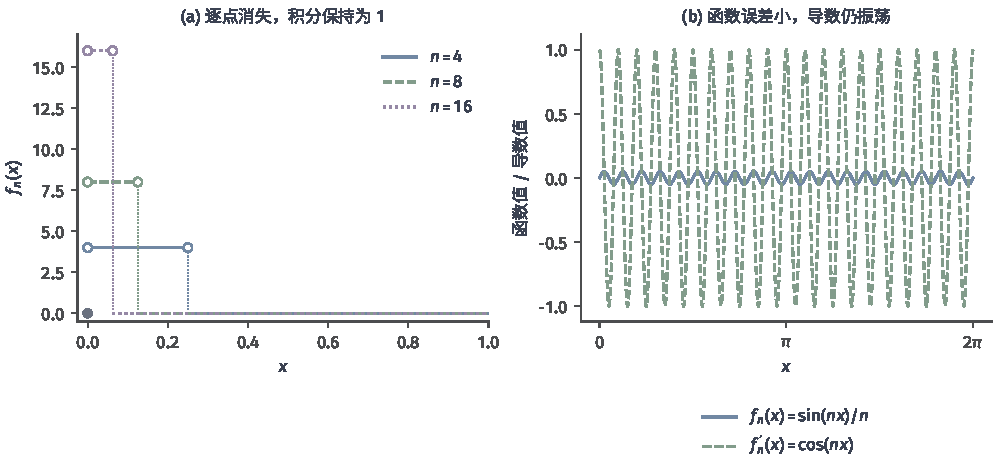
\includegraphics[width=169.0mm]{figures/00-shared/mathematical-preliminaries-upper/03-calculus/matplotlib/analysis-convergence-obstacles/figure.pdf}
  \caption{两种交换运算的障碍。左图的尖峰支撑不断收缩，但高度同步增长，每条曲线的积分仍为$1$；开圆点标出不取的上端点，竖虚线仅提示跳跃。右图取$n=20$，$\sin(nx)/n$的函数幅度很小，导数$\cos(nx)$仍有单位幅度。两图均为按给定函数公式构造的教学示例。}
 \label{fig:analysis-convergence-obstacles}
\end{figure*}

表~\ref{tab:analysis-interchange-conditions}汇总极限与勒贝格积分交换的不同条件。积分等式成立的依据来自这些条件，不能仅由点态极限的存在推出。
\begin{table*}[htbp]
 \centering\small
 \begin{tabularx}{\linewidth}{@{}lXX@{}}
 \toprule
 结果 & 核对的条件 & 可得到的结论\\
 \midrule
 有限测度上一致收敛 & 各项可积，且全部输入的误差一致趋零 & 极限可积，积分可交换极限\\
 单调收敛 & 非负可测函数逐点或几乎处处递增 & 极限与积分相等，允许无穷值\\
 Fatou引理 & 非负可测函数列 & 先取下极限再积分，不超过先积分再取下极限的结果\\
 支配收敛 & 几乎处处收敛，且共用一个可积绝对上界 & 积分可交换极限，并有$\int|f_n-f|\,\mathrm dm\to0$\\
 \bottomrule
 \end{tabularx}
 \caption{极限与勒贝格积分之间的交换条件。表中的测度、可测性和统一控制属于结论的假设。}
 \label{tab:analysis-interchange-conditions}
\end{table*}


本小节的三类结论控制的运算不同：保留连续性需要共同的函数值误差，交换微分还要控制导数，交换积分则要检查有限测度、非负单调性或共同可积支配等相应条件。表~\ref{tab:analysis-interchange-conditions}中的条件及前面的反例给出了各自的适用边界。

\subsection{函数项级数的极限}
\label{sec:analysis-function-series-limits}

函数列的极限比较一列已经给定的函数；函数项级数则把不断加入的函数项累计起来。
给定$u_n:X\to\mathbb R$，记部分和$S_N(x)=\sum_{n=1}^Nu_n(x)$，研究$\sum_{n=1}^\infty u_n(x)$就是研究函数列$(S_N)$。
下面先按部分和区分收敛方式，再判断何时收敛，以及求导或积分能否移入无穷求和。

\subsubsection{收敛方式与判别}

部分和把级数化成函数列，前面几种收敛方式都可以沿用，但必须说明它们约束的是部分和，而不是单个函数项$u_n$。
下面逐一给出定义；判据则是把函数列的柯西判据用于部分和。

\paragraph{点态收敛}
固定输入后，函数项级数就是一个数项级数，点态收敛要求每个这样的数项级数都收敛。
\begin{definition}[函数项级数的点态收敛]
\label{def:analysis-series-pointwise-convergence}
设$X\subseteq\mathbb R$，$u_n:X\to\mathbb R$，$S_N=\sum_{n=1}^Nu_n$。若存在$u:X\to\mathbb R$，使部分和$S_N$在$X$上点态收敛到$u$，即对每个$x\in X$都有$\sum_{n=1}^\infty u_n(x)=u(x)$，就称函数项级数$\sum_nu_n$在$X$上点态收敛，$u$称为它的和函数。
\end{definition}
尾部起点可以随$x$改变。特别地，$u_n(x)\to0$只是必要条件，不能代替部分和收敛。

\paragraph{点态收敛的判据}
未知和函数时，比较两个较晚的部分和；它们的差是一段有限尾和，因此点态收敛等价于
\[
 \begin{gathered}
 \forall x\in X,\quad\forall\varepsilon>0,\quad\exists N=N(x,\varepsilon),\\
 m>n\geq N\Longrightarrow
 \left|\sum_{k=n+1}^{m}u_k(x)\right|<\varepsilon.
 \end{gathered}
\]
这是将定理~\ref{thm:analysis-pointwise-cauchy-criterion}用于$S_N$，与对数项级数逐点使用柯西准则完全一致。

\paragraph{一致收敛}
若希望同一个项数同时控制全部输入处的截断误差，就要求部分和一致收敛。
\begin{definition}[函数项级数的一致收敛]
\label{def:analysis-series-uniform-convergence}
设$\sum_nu_n$在$X$上点态收敛到和函数$u$。若部分和$S_N$在$X$上一致收敛到$u$，即
\[
 \sup_{x\in X}\left|u(x)-\sum_{n=1}^Nu_n(x)\right|\longrightarrow0\qquad(N\to\infty),
\]
就称函数项级数在$X$上一致收敛。
\end{definition}
同一个$N$控制全部输入处的剩余和。例如在$[0,1)$上，$\sum_{n=0}^\infty x^n$逐点收敛到$1/(1-x)$，但收敛不一致：若一致收敛，可取$N$使$|u-S_N|<1$在$[0,1)$上成立，有界的部分和$S_N$便迫使和函数$u\leq S_N+1$有界，与$1/(1-x)$无界矛盾。
若每个$u_n$连续，有限部分和也连续，一致收敛便由定理~\ref{thm:analysis-uniform-continuity-limit}保证和函数连续。

\paragraph{一致收敛的判据}
若希望得到一致收敛，就要把尾部起点的选择放在选择输入之前。
由定理~\ref{thm:analysis-uniform-cauchy-criterion}，一致收敛当且仅当
\[
 \begin{gathered}
 \forall\varepsilon>0,\quad\exists N,\quad\forall x\in X,\\
 m>n\geq N\Longrightarrow
 \left|\sum_{k=n+1}^{m}u_k(x)\right|<\varepsilon.
 \end{gathered}
\]
这里不预先指定和函数：实数的完备性先提供各点的极限，共同的尾和界再使收敛一致。

\paragraph{几乎处处收敛}
积分只关心零测集之外的取值，因此也可以只要求部分和在零测集之外收敛。
\begin{definition}[函数项级数的几乎处处收敛]
\label{def:analysis-series-almost-everywhere-convergence}
设$E\in\mathcal L(\mathbb R)$，$u_n:E\to\mathbb R$可测。若存在零测集$N_0\subseteq E$，使对每个$x\in E\setminus N_0$，部分和$S_N(x)$都收敛到有限值$u(x)$，就称$\sum_nu_n$在$E$上几乎处处收敛到$u$。
\end{definition}
可以把和函数在$N_0$上取为零，它仍可测。几乎处处收敛与点态收敛的区别是允许一个固定的零测例外，它并未提供全域共同的误差界。

\paragraph{绝对收敛}
正负项相消可能使部分和收敛，而绝对值级数仍发散；绝对收敛排除了这种相消。
\begin{definition}[函数项级数的绝对收敛]
\label{def:analysis-series-absolute-convergence}
若对每个$x\in X$，数项级数$\sum_n|u_n(x)|$都收敛，就称级数$\sum_nu_n$在$X$上绝对收敛。若$X=E$是可测集，而这一条件只在某个零测集之外成立，就称该级数几乎处处绝对收敛。
\end{definition}
由数项级数的绝对收敛判别，绝对收敛能保证相应位置的级数收敛，却不自动给出一致收敛；后者还需要对全部输入共同适用的尾和控制。例如$\sum_{n\geq0}x^n$在$[0,1)$上每点绝对收敛，却不一致收敛。

\paragraph{Weierstrass判别法}
逐一估计所有输入处的尾和可能很困难。若每一项都能用一个与输入无关的非负数控制，就可以把函数项级数归约为已知的数项级数。
\begin{theorem}[Weierstrass判别法]
\label{thm:analysis-weierstrass-series-test}
设$X$非空，$u_n:X\to\mathbb R$。若存在非负实数$M_n$使
\[
 \forall x\in X,\quad |u_n(x)|\leq M_n,
 \qquad \sum_{n=1}^{\infty}M_n<\infty,
\]
则$\sum_nu_n$在每个$x$处绝对收敛，并在$X$上一致收敛到某个实值函数$u$。
此外，截断误差满足
\[
 \sup_{x\in X}\left|u(x)-\sum_{n=1}^Nu_n(x)\right|
 \leq\sum_{n>N}M_n\longrightarrow0.
\]
\end{theorem}
\begin{proof}
对每个固定$x$，比较判别给出$\sum_n|u_n(x)|\leq\sum_nM_n<\infty$，故和$u(x)$存在。
对任意$m>N$，三角不等式给出$|\sum_{n=N+1}^m u_n(x)|\leq\sum_{n>N}M_n$。
令$m\to\infty$并对$x$取上确界，就得到所述误差界；数项级数的尾和趋零，故收敛一致。
\end{proof}
例如在$[-1,1]$上，$u_n(x)=x^n/2^n$满足$|u_n(x)|\leq2^{-n}$，而$\sum_{n>N}2^{-n}=2^{-N}$。
这个共同的几何尾和控制全部输入处的截断误差；每个函数项连续，所以和函数也连续。
判别法只是充分条件，不能把“没有找到这样的$M_n$”当成不一致收敛的证明。

\subsubsection{逐项求导}

部分和总可以有限次求导，问题在于求导后再取极限，是否得到和函数的导数。
仅有原级数一致收敛还不够；下面把控制施加在导数级数上，并用一个点的函数值确定累计常数。
\begin{theorem}[函数项级数的逐项求导]
\label{thm:analysis-function-series-differentiation}
设$u_n\in C^1([a,b])$。若存在$x_0\in[a,b]$使$\sum_nu_n(x_0)$收敛，且导数级数$\sum_nu_n'$在$[a,b]$上一致收敛，则$\sum_nu_n$在$[a,b]$上一致收敛到某个$u\in C^1([a,b])$，且
\[
 u'(x)=\sum_{n=1}^{\infty}u_n'(x).
\]
\end{theorem}
\begin{proof}
取$S_N=\sum_{n=1}^Nu_n$，则$S_N(x_0)$收敛，$S_N'=\sum_{n=1}^Nu_n'$一致收敛。
将函数列导数的一致收敛结论（定理~\ref{thm:analysis-uniform-derivative-limit}）用于$S_N$，即得原级数一致收敛、和函数连续可微以及导数公式。
\end{proof}
实际验证时，常对导数级数$\sum_nu_n'$使用Weierstrass判别法；要找的是$|u_n'|$的共同上界，而不是$|u_n|$的共同上界。
若函数项只有绝对连续性，也可将定理~\ref{thm:analysis-integral-derivative-limit}用于部分和：单点处的级数收敛，且导数部分和按绝对误差积分趋于某个可积函数$g$时，和函数绝对连续，并有$u'=g$几乎处处。
这里$g$是导数部分和在积分误差意义下的极限，不能额外断言导数级数在每个点都收敛。

\subsubsection{逐项积分}

有限部分和的积分总可以写成有限和，能否再令项数趋于无穷，则取决于对部分和积分的控制。
非负项、绝对积分的总和有限以及有限测度上的一致收敛，给出三种不同的充分条件。以下设$E\in\mathcal L(\mathbb R)$。

\paragraph{非负函数项级数的逐项积分}
非负项使部分和递增，因此可以直接使用单调收敛定理，不要求总积分有限。
\begin{theorem}[非负函数项级数的逐项积分]
\label{thm:analysis-nonnegative-series-integration}
若$u_n:E\to[0,\infty]$可测，则
\[
 \int_E\sum_{n=1}^{\infty}u_n\,\mathrm dm
 =\sum_{n=1}^{\infty}\int_Eu_n\,\mathrm dm,
\]
两边均允许为$+\infty$。
\end{theorem}
\begin{proof}
非负部分和$S_N$递增到$\sum_nu_n$。用单调收敛定理交换极限与积分，再对每个$S_N$用有限加法，即得等式。
\end{proof}

\paragraph{绝对积分总和有限时的逐项积分}
有正负项时，绝对值的累计可以同时控制无穷求和中的抵消及积分误差。
下面的条件既保证和函数可积，也保证部分和按绝对误差积分趋于和函数。
\begin{theorem}[绝对积分可求和的函数项级数]
\label{thm:analysis-absolutely-integrable-series}
若$u_n:E\to\mathbb R$可测且$\sum_n\int_E|u_n|\,\mathrm dm<\infty$，则$\sum_nu_n$几乎处处绝对收敛。
将和函数在绝对值级数发散的零测集上定义为零，所得$u$可积，并有
\[
 \int_E\left|u-\sum_{n=1}^Nu_n\right|\,\mathrm dm
 \leq\sum_{n>N}\int_E|u_n|\,\mathrm dm\longrightarrow0,
\]
从而
\[
 \int_Eu\,\mathrm dm=\sum_{n=1}^{\infty}\int_Eu_n\,\mathrm dm.
\]
\end{theorem}
\begin{proof}
由非负级数的逐项积分，$G=\sum_n|u_n|$满足$\int_EG\,\mathrm dm<\infty$，故$G<\infty$几乎处处。
在零测集$N_0=\{G=\infty\}$之外，级数绝对收敛，且$|u|\leq G$；在$N_0$上取$u=0$后，$u$仍可测且可积。
对几乎每个$x$，$|u(x)-S_N(x)|\leq\sum_{n>N}|u_n(x)|$。
对这一不等式积分，再对右侧的非负尾级数逐项积分，得到所述误差界。
积分之差不超过绝对误差的积分，而有限部分和满足$\int S_N=\sum_{n=1}^N\int u_n$，令$N\to\infty$便得到结论。
\end{proof}

\paragraph{有限测度上一致收敛时的逐项积分}
还有一种充分条件直接约束部分和的共同误差，而不要求绝对积分的总和有限。
若$m(E)<\infty$、各$u_n$可积，且部分和$S_N$一致收敛到$u$，则定理~\ref{thm:analysis-uniform-lebesgue-integral-limit}给出
\[
 \int_Eu\,\mathrm dm
 =\lim_{N\to\infty}\int_ES_N\,\mathrm dm
 =\sum_{n=1}^{\infty}\int_Eu_n\,\mathrm dm.
\]
这里的关键是有限总测度乘一致误差趋零；它与定理~\ref{thm:analysis-absolutely-integrable-series}的绝对可求和条件是两项不同的条件，应分别检查。

\subsection{反常积分}
\label{sec:analysis-improper-integrals}

前面的有限区间计算还留下两个问题：积分范围延伸到无穷远时怎样累计，函数在端点或内部某点附近无界时怎样累计。
这两类问题通常称为\term{反常积分}（improper integral）。下面先分别说明定义与截断方式，再集中判断何时可积。
本小节沿用勒贝格积分的约定：非负函数的积分允许为无穷，有符号函数的有限可积性要求绝对值的积分有限；截断只用来计算已有的积分，不把按指定顺序得到的抵消另算作有限的勒贝格积分。

\subsubsection{无穷区间上反常积分的定义}

先设$f$在每个有限区间$[a,R]$上勒贝格可积，唯一待处理的是无穷远处的尾部。
把积分范围延伸到半轴，就得到这一类反常积分的记号。
\begin{definition}[无穷区间上的反常积分]
\label{def:analysis-improper-infinite-interval}
设$f:[a,\infty)\to\mathbb R$可测，且在每个$[a,R]$上可积。
将$[a,\infty)$上的勒贝格积分记为
\[
 \int_a^\infty f(x)\,\mathrm dx:=\int_{[a,\infty)}f\,\mathrm dm,
\]
称为无穷区间上的反常积分。
若$f\geq0$，该值属于$[0,\infty]$；若$f$有正负值，本节讨论其有限积分时要求$\int_a^\infty|f|<\infty$。
\end{definition}
这个记号可以通过有限范围上的计算求值。非负时由单调收敛定理，有
\[
 \int_a^\infty f(x)\,\mathrm dx
 =\lim_{R\to\infty}\int_a^R f(x)\,\mathrm dx,
\]
允许为无穷；有符号且绝对可积时，以$|f|$为支配函数，对$f\mathbb I_{[a,R]}$使用支配收敛定理，也得到同一有限等式。
严格说，两个收敛定理先沿一列$R_n\uparrow\infty$使用；非负累计关于$R$的单调性，或遗漏范围上绝对积分趋零，再保证任意方式的$R\to\infty$都得到相同结论。

左半轴作相同处理。整个实轴上还需分别处理左右两端：对任意固定的$c\in\mathbb R$，$f$可积当且仅当两侧的绝对值积分都有限，此时
\[
 \int_{\mathbb R}f\,\mathrm dm
 =\int_{(-\infty,c]}f\,\mathrm dm+\int_{(c,\infty)}f\,\mathrm dm.
\]
只知道对称截断$[-R,R]$中的正负抵消稳定，不能代替左右两侧可积，示例~\ref{ex:analysis-sign-function-no-integral}已经说明这一点。

\subsubsection{无界函数反常积分的定义}

范围有限时，函数仍可能在端点附近无界。先避开该端点计算，再检查遗漏的短区间是否保留了不可忽略的累计。
\begin{definition}[无界函数的反常积分]
\label{def:analysis-improper-unbounded-function}
设$f:(a,b]\to\mathbb R$可测，在每个$[c,b]$（$a<c<b$）上可积，并允许在$a$附近无界。
将$(a,b]$上的勒贝格积分记为
\[
 \int_a^bf(x)\,\mathrm dx:=\int_{(a,b]}f\,\mathrm dm,
\]
称为在端点$a$处的反常积分。
若$f\geq0$，该值允许为$+\infty$；若$f$有正负值，本节讨论其有限积分时要求$\int_{(a,b]}|f|\,\mathrm dm<\infty$。
\end{definition}
非负时，$f\mathbb I_{[c,b]}$随$c\downarrow a$逐步增加到$f$；有符号且绝对可积时，这些截断函数由$|f|$支配。
因此分别用单调收敛定理或支配收敛定理得到
\[
 \int_{(a,b]}f\,\mathrm dm=\lim_{c\downarrow a}\int_c^bf(x)\,\mathrm dx.
\]
若无界位置在右端点，就从左侧截断；若在内部点$s$，则把$(a,s)$与$(s,b)$分开累计，有符号的有限积分要求两侧均绝对可积。
在单点上赋予有限值不改变勒贝格积分，因而决定可积性的是该点附近的累计，而不是该点取了什么值。


图~\ref{fig:analysis-process-improper-two-truncations}对照两种截断：向外扩大累计范围，或从奇点附近逐渐补回遗漏的范围。
\begin{figure*}[!htbp]
 \centering
 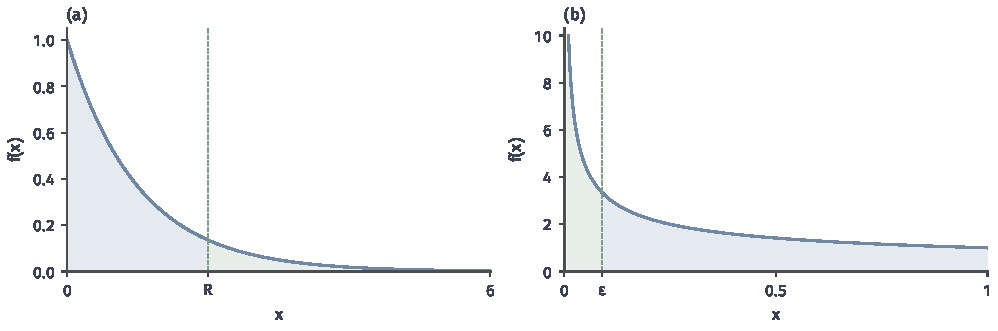
\includegraphics[width=169.0mm]{figures/00-shared/mathematical-preliminaries-upper/00-shared/matplotlib/chapter3-concept-processes/improper-two-truncations.pdf}
 \caption{(a) $e^{-x}$在$[0,\infty)$上，以$R=2$截断，蓝区已计入，绿区属于遗漏尾部，其完整积分为$e^{-2}$；图只显示到$x=6$。(b) $x^{-1/2}$在$(0,1]$上，以$\varepsilon=0.09$截断，完整遗漏积分为$2\sqrt\varepsilon$。右图曲线只绘$x\geq0.01$，未画出的更近零点部分仍属积分范围。}
 \label{fig:analysis-process-improper-two-truncations}
\end{figure*}

\subsubsection{反常积分的可积性}

两种截断都可以写为递增的可测范围$E_n\uparrow E$：范围不断向外延伸，或者从被避开的奇异位置逐步收回遗漏的部分。
因此可以用同一个判据回答可积性问题，随后再用截断积分或原函数计算具体数值。

\paragraph{简单函数与截断函数的积分收敛}
函数列的收敛定理补上了前面几种逼近中积分极限的依据。对非负可测$f$，规范简单逼近$s_n$逐点递增到$f$，单调收敛定理给出$\int s_n\uparrow\int f$。

若$f$绝对可积，按高度截断的$f_n=\max\{-n,\min\{f,n\}\}$满足$f_n\to f$且$|f_n|\leq|f|$，支配收敛定理给出$\int|f_n-f|\to0$。
在实轴上按范围截断的$f\mathbb I_{[-n,n]}$同样被$|f|$支配。这与前面的无穷范围截断相对应，说明有限范围上的计算可以逼近全域上的积分。

\paragraph{非负函数的可积性}
非负累计随截断范围扩大而增加，积分有限的关键在于这些累计能否被同一个有限常数控制。
\begin{theorem}[非负截断累计的有界判据]
\label{thm:analysis-improper-nonnegative-criterion}
设$E\in\mathcal L(\mathbb R)$，$f:E\to[0,\infty]$可测，$E_n$为递增可测集且$\bigcup_nE_n=E$。则
\[
 \int_Ef\,\mathrm dm<\infty
 \quad\Longleftrightarrow\quad
 \sup_n\int_{E_n}f\,\mathrm dm<\infty,
\]
并有$\int_Ef\,\mathrm dm=\lim_n\int_{E_n}f\,\mathrm dm$。
\end{theorem}
\begin{proof}
因为$0\leq f\mathbb I_{E_n}\uparrow f$，单调收敛定理使全域积分等于截断积分序列的极限，也就是其上确界。
因此全域积分有限恰好等价于这些截断积分有共同的有限上界。
\end{proof}
在无穷半轴上可取$E_n=[a,a+n]$，在奇异端点$a$附近可取$E_n=[a+(b-a)/(n+1),b]$。
只知道每一个截断积分分别有限还不够，还要检验它们是否有共同的上界。

由积分的单调性还得到比较原则：若$0\leq f\leq g$几乎处处且$\int g<\infty$，则$\int f<\infty$；反之，若$0\leq g\leq f$且$\int g=\infty$，则$\int f=\infty$。
最基本的比较对象是幂函数，它们的截断积分可以用原函数算出。
\begin{example}[用截断计算幂函数的反常积分]
\label{ex:analysis-power-integral-truncations}
在$(0,1]$上取$E_n=[1/n,1]$。由原函数$2\sqrt x$与$\log x$，
\[
 \int_{1/n}^1x^{-1/2}\,\mathrm dx=2(1-n^{-1/2})\longrightarrow2,
 \qquad
 \int_{1/n}^1x^{-1}\,\mathrm dx=\log n\longrightarrow+\infty.
\]
由定理~\ref{thm:analysis-improper-nonnegative-criterion}，$\int_0^1x^{-1/2}\,\mathrm dx=2$，而$\int_0^1x^{-1}\,\mathrm dx=+\infty$。
在$[1,\infty)$上取$E_n=[1,n]$，同理有$\int_1^nx^{-2}\,\mathrm dx=1-1/n\to1$与$\int_1^nx^{-1}\,\mathrm dx=\log n\to+\infty$，所以$\int_1^\infty x^{-2}\,\mathrm dx=1$，而$\int_1^\infty x^{-1}\,\mathrm dx=+\infty$。
\end{example}
这几项计算始终使用同一个勒贝格积分定义，极限等式由单调收敛定理保证。

同一个幂函数在奇点附近与在无穷远处的可积条件恰好相反。不求原函数，也可以用二进分段与几何级数判断$x^{-p}$在两端的可积性。
\begin{example}[幂函数$x^{-p}$的可积阈值]
\label{ex:analysis-power-integrability-thresholds}
先看无穷远处。对$p>0$，$x^{-p}$在$[2^k,2^{k+1}]$上递减，把它在该段的最小值和最大值分别乘以区间长度$2^k$，得到
\[
 2^{-p}2^{k(1-p)}\leq\int_{2^k}^{2^{k+1}}x^{-p}\,\mathrm dx\leq2^{k(1-p)}.
\]
由区域可加性，$\int_1^\infty x^{-p}\,\mathrm dx$等于这些分段积分对$k\geq0$之和。$p>1$时上界$2^{k(1-p)}$是公比小于一的几何数列，部分和有共同上界$1/(1-2^{1-p})$，所以积分有限；$0<p\leq1$时每段至少贡献$2^{-p}$，累计发散。$p\leq0$时在$x\geq1$上$x^{-p}\geq1$，也发散。

再看零点附近。对$p>0$，比较$[2^{-(k+1)},2^{-k}]$上的最小值与最大值，得到该段积分介于$2^{k(p-1)}/2$与$2^{p-1}2^{k(p-1)}$之间；这组几何数列的公比为$2^{p-1}$，所以对$k\geq0$求和恰在$p<1$时有限。$p\leq0$时$x^{-p}$在$(0,1]$上有界（可连续延拓到$0$），本来就可积。

于是$\int_0^1x^{-p}\,\mathrm dx$恰在$p<1$时有限，$\int_1^\infty x^{-p}\,\mathrm dx$恰在$p>1$时有限。
\end{example}
分段常数比较与几何级数给出可积性的阈值，原函数则能进一步算出有限截断的具体数值；$p=1/2$与$p=2$的结果与示例~\ref{ex:analysis-power-integral-truncations}一致。

\paragraph{有符号函数的可积性}
正负值抵消可能使截断积分保持有限，但可积性要求正、负两部分各自具有有限的累计。
因此应把定理~\ref{thm:analysis-improper-nonnegative-criterion}的非负判据用于$|f|$，而不是用于有正负抵消的$f$。
\begin{theorem}[绝对截断累计的可积性判据]
\label{thm:analysis-improper-signed-criterion}
设$E\in\mathcal L(\mathbb R)$，$f:E\to\mathbb R$可测，$E_n\uparrow E$为可测范围，则$f$可积当且仅当
\[
 \sup_n\int_{E_n}|f|\,\mathrm dm<\infty.
\]
可积时，每个截断积分有限，且
\[
 \left|\int_Ef\,\mathrm dm-\int_{E_n}f\,\mathrm dm\right|
 \leq\int_{E\setminus E_n}|f|\,\mathrm dm\longrightarrow0.
\]
所以任意这样的递增穷尽都得到同一个积分值。
\end{theorem}
\begin{proof}
将非负截断判据用于$|f|$，即得充要条件。可积时，区域可加性把积分之差写成遗漏范围上的积分，再用绝对值界得到误差不等式。
函数$|f|\mathbb I_{E\setminus E_n}$逐点趋零且由可积的$|f|$支配，故其积分趋零。
\end{proof}
绝对值尾部既用于判断可积性，也控制有限计算的误差。

例如$p>1$时，把$x^{-p}$在$[1,\infty)$上截断到$[1,R]$（$R>1$），由区域可加性，截断误差恰为尾部积分$\int_R^\infty x^{-p}\,\mathrm dx$，它正是定理~\ref{thm:analysis-improper-signed-criterion}中误差界的右侧。按$[2^jR,2^{j+1}R]$分段比较，得到
\[
 \int_R^\infty x^{-p}\,\mathrm dx
 \leq R^{1-p}\sum_{j=0}^\infty2^{j(1-p)}
 =\frac{R^{1-p}}{1-2^{1-p}}\longrightarrow0.
\]
非负积分的可数区域可加性保证分段求和合法，几何尾和给出显式的误差界。

函数列极限部分留下了一个问题：可积的支配函数本身可以无界。有了$x^{-1/2}$的可积性，就能核对这样的例子。
\begin{example}[无界的可积支配函数]
\label{ex:analysis-unbounded-dominating}
在$(0,1)$上令$f_n(x)=x^n/\sqrt x=x^{n-1/2}$。对每个$x\in(0,1)$，$f_n(x)\to0$；并且$0\leq f_n\leq x^{-1/2}$。
支配函数$x^{-1/2}$在$0$附近无界，但由示例~\ref{ex:analysis-power-integral-truncations}，$\int_0^1x^{-1/2}\,\mathrm dx=2<\infty$，所以支配收敛定理保证$\int_0^1f_n\,\mathrm dx\to0$。
直接计算也得到同一结论：截断后用原函数，$\int_0^1x^{n-1/2}\,\mathrm dx=(n+1/2)^{-1}\to0$。
\end{example}
支配条件要求共同上界的积分有限，不要求上界本身有界。

积分有限要求正负两部分都有限，不能从某一列截断积分有有限极限直接推出。
下面两个例子只说明这种推断为什么失效，不把截断相消作为新的积分规则。先看连续函数在无穷区间上的截断相消。
\begin{example}[$\sin x/x$的截断极限存在但不绝对可积]
\label{ex:analysis-sine-over-x}
在$[1,\infty)$上，取$u(x)=1/x$、$v'(x)=\sin x$作分部积分，得到
\[
 \int_1^R\frac{\sin x}{x}\,\mathrm dx
 =\cos1-\frac{\cos R}{R}-\int_1^R\frac{\cos x}{x^2}\,\mathrm dx.
\]
$R\to\infty$时端点项$\cos R/R\to0$；最后一项的被积函数满足$|\cos x/x^2|\leq x^{-2}$，绝对可积，由定理~\ref{thm:analysis-improper-signed-criterion}收敛到有限值。所以截断积分存在有限极限。
但在每个$[k\pi+\pi/6,k\pi+5\pi/6]$（$k\geq1$）上，$|\sin x|\geq1/2$且$x\leq(k+1)\pi$，区间长为$2\pi/3$，故该段的绝对积分至少为$1/(3(k+1))$。
这些区间两两不交，调和级数发散，所以$\int_1^\infty|\sin x|/x\,\mathrm dx=+\infty$。
\end{example}
这个有限的截断极限依赖正负抵消，不是本章所用的有限勒贝格积分。

奇点两侧的抵消也有同样的问题。
\begin{example}[$1/x$的柯西主值]
\label{ex:analysis-cauchy-principal-value}
在$(-1,1)$上取$f(x)=1/x$，原点处赋值为零。
由示例~\ref{ex:analysis-power-integral-truncations}，$\int_0^1x^{-1}\,\mathrm dx=+\infty$，对称地负部在$(-1,0)$上的积分也为无穷，所以$f$没有有符号勒贝格积分。
但对称截断满足
\[
 \lim_{\varepsilon\downarrow0}\left(
 \int_{-1}^{-\varepsilon}\frac{\mathrm dx}{x}
 +\int_{\varepsilon}^{1}\frac{\mathrm dx}{x}\right)
 =\lim_{\varepsilon\downarrow0}\bigl(\log\varepsilon-\log\varepsilon\bigr)=0.
\]
若改用非对称截断$\int_{-1}^{-\varepsilon}+\int_{2\varepsilon}^1$，两项之和恒为$\log\varepsilon-\log(2\varepsilon)=-\log2$，极限变为$-\log2$。
\end{example}
对称相消的极限称为柯西主值。它的数值依赖截断方式，没有使$\int|f|$变为有限，也没有定义出本章采用的勒贝格积分。
后续计算仍只使用非负函数的积分（允许为无穷）或绝对可积函数的有限积分。

\FloatBarrier


\FloatBarrier
\section{本章小结}
\label{sec:measurable-summary}

有限个区间的并只能逼近一部分集合，由此得到Jordan测量；改用可数个区间覆盖，就得到勒贝格外测度。精确分割条件从全部子集中选出可测集，外测度限制在可测集上满足可数可加性，这就是勒贝格测度。
单调性、次可加性和集合列的连续性都由可数可加性推出。零测集给出“几乎处处”的例外语言；康托尔集说明零测集可以含有不可数多个点，康托尔函数说明全部增长可以集中在一个零测集上。

黎曼积分从区间分割出发，勒贝格积分按可测集合与简单函数累计。有界区间上的黎曼可积函数也勒贝格可积，积分值相同；反过来不成立，狄利克雷函数就是例子。
不定积分由原函数定义，变上限积分由累计构造，二者的联系要靠微积分基本定理建立。被积函数连续时，累计函数在每一点都以它为导数；被积函数只是勒贝格可积时，只能保证几乎处处如此。反方向上，函数可以由导数的积分恢复，恰好当它绝对连续；康托尔函数说明一致连续还不够。

函数列一致收敛时，连续函数的极限仍连续；要交换极限与求导，还需控制导数；要交换极限与积分，还需有限测度上的一致收敛、非负单调性或共同的可积上界。
无穷区间与无界函数上的积分仍按同一个勒贝格积分定义计算，截断只是求值的手段；可积性由绝对值的累计是否有限决定，指定方式下的相消极限不能代替可积性。

